\documentclass[letterpaper, 10pt, conference]{ieeeconf} % Change font size to 9pt

\IEEEoverridecommandlockouts
\overrideIEEEmargins

\usepackage{graphics}
\usepackage{epsfig}
% \usepackage{mathptmx}
% \usepackage{times}
\usepackage{amsmath}
\usepackage{amssymb}
% \usepackage{cite}
\usepackage{lpic}
\usepackage{overpic}
% \usepackage{blkarray}
\usepackage{mathrsfs}
\usepackage{todonotes}
\usepackage[hidelinks]{hyperref}
\usepackage{caption}

\usepackage{tikz}
\usetikzlibrary{arrows,positioning,patterns,decorations.pathreplacing,calc,shapes.geometric}

\usepackage[backend=biber,
			sortcites=true,
			sorting=none,
			style=numeric-comp,
			firstinits=true,
			doi=false,
			isbn=false,
			url=false
			]{biblatex}
\bibliography{MyBib}


% \DeclareNameFormat{author}{%
%   \ifthenelse{\value{listcount}=1}
%     {\namepartfamily%
%      	\ifblank{\namepartgiven}{}{
% 		\addcomma\space\namepartgiven}}
% 	{\ifblank{\namepartgiven}{}{\namepartgiven\space}%
%    		\namepartfamily}%
% 		\ifthenelse{\value{listcount}<\value{liststop}}
%   	{\addcomma\space}{}
% }

\newcommand*{\Resize}[1]{\resizebox{\columnwidth}{!}{$#1$}}

\newtheorem{thm}{Lemma}[section]
\newtheorem{rem}[thm]{Remark}
\newtheorem{defn}[thm]{Definition}
\newtheorem{assn}{Assumption}
\newtheorem{algo}[thm]{Algorithm}

\providecommand{\norm}[1]{\left\|#1\right\|}
\providecommand{\abs}[1]{\left\lvert#1\right\rvert}
\providecommand{\conv}{\text{conv}}
\providecommand{\bfa}[1]{\mathbf{#1}}

\usepackage{parskip}
\setlength{\parskip}{8pt} 
\setlength{\parindent}{0pt}

\usepackage{xcolor}
\def\edit{\textcolor{blue}}
\allowdisplaybreaks[4]


\DeclareFontFamily{U}{mathx}{\hyphenchar\font45}
\DeclareFontShape{U}{mathx}{m}{n}{
      <5> <6> <7> <8> <9> <10> gen * mathx
      <10.95> mathx10 <12> <14.4> <17.28> <20.74> <24.88> mathx12
      }{}
\DeclareSymbolFont{mathx}{U}{mathx}{m}{n}
\DeclareFontSubstitution{U}{mathx}{m}{n}
\DeclareMathSymbol{\temp}{\mathbin}{mathx}{'341}
\newcommand{\bigominus}{\raisebox{10pt}{$\temp$}}

\DeclareMathOperator*{\maximize}{maximize}
\DeclareMathOperator*{\minimize}{minimize}

\graphicspath{{./Pix/}}

\begin{document}
\title{A set based approach to chance constrained programming}

\author{Rainer M. Schaich\textsuperscript{\dag} %
         and Mark Cannon\textsuperscript{\dag,\ddag}%
\thanks{\textsuperscript{\dag} Department of Engineering Science, University of Oxford, OX1 3PJ.}%
\thanks{\textsuperscript{\ddag} Corresponding author, 
        \texttt{mark.cannon@eng.ox.ac.uk}.}
}
\newcommand{\note}[1]{\todo[inline]{#1}}

\maketitle

\begin{abstract} 
For a certain class of stochastic programming problems we introduce a method to robustify the problem and thereby reduce the complexity while introducing a minimal amount of uncertainty.
%
An optimal auxiliary polytope is determined using a nonlinear optimisation program, this auxiliary set can then be used to solve a deterministic problem guaranteeing probabilistic constraint satisfaction.
%
We furthermore present a method to determine the probability measure of a polytope efficiently using Riemann-like sums over a grid.
%
Methods to generate both homogeneous and inhomogeneous grids are presented.
%
The proposed scheme is illustrated and compared with state-of-the-art alternatives in an example.
\end{abstract}

\begin{keywords}
keyword 1, keyword 2, keyword 3...
\end{keywords}
%%%%%%%%%%%%%%%%%%%%%%%

\section{Introduction}\label{sec:intro}%
%
%
%
%
%
\noindent Optimisation problems with probabilistic constraints on the decision variable arise in various domains of science.
%
A prominent approach to solving such problems is to employ a scenario based approach~\cite{Calafiore:2010}, for which a deterministic optimisation program is solved for a sufficiently large number of sampled probabilistic constraints.
%
This way constraint satisfaction with a chosen confidence is guaranteed, however the number of samples necessary generally depends on the dimension, the desired probability and confidence level and is often unnecessarily large.
%
In cases for which we have more particular knowledge of the meaning of the probabilistic constraints it is often possible to reformulate the stochastic problem as a robust optimisation problem which can be solved using existing methods.
%
The trivial way would be to satisfy the probabilistic constraints with certainty, which reduces the complexity of the problem but increases the conservatism of its solution.
%
Here we present a more sophisticated approach, we determine an auxiliary subset of the uncertain variable for which the probabilistic constraints are satisfied.
%

To be able to determine such auxiliary sets we have to constrain the search space to polytopes of a given combinatorial structure.
%
This allows us to formulate a nonlinear programming problem to determine an optimal auxiliary set which can then be used to robustify the original stochastic program introducing a minimal amount of conservatism.
%
We present a method to approximate the probability measure of the auxiliary set in a computationally tractable way using a grid based discretisation of the probability space.
%


%
This paper is structured as follows:
%
In Section~\ref{sec:problem:formulation} we present the problem description we consider, Section~\ref{sec:optimising:polytopes} discusses the proposed method to reduce the uncountably infinite dimensional optimisation problem introduced in Section~\ref{sec:problem:formulation} to a finite dimensional nonlinear optimisation program.
%
Section~\ref{sec:counting:cubes} deals with the problem of approximating the probability measure of a polytope using a homogeneous discretisation of the probability space, thereby reducing integrals into finite sums which can be efficiently evaluated.
%
We illustrate the proposed scheme in Section~\ref{sec:example} and compare the result with a scenario-based method.
%
A method to determine a inhomogeneous discretisation of the probability space is presented in Section~\ref{sec:improved:grid}.
%
Section~\ref{sec:conclusion} concludes this work and gives possible future directions of research.
%


%
Throughout the paper we use the term \textit{$d$-dimensional polytope} to refer to a bounded set containing a $d$-dimensional ball and formed by the intersection of a finite number of halfspaces or equivalently by the convex hull of a finite number of points.
A \textit{face} of a polytope is its intersection with a hyperplane such that the polytope lies on one side of the hyperplane; the dimension of the face is the dimension of the affine hull of this intersection; one-, two- and ${(d-1)}$-dimensional faces are called \textit{vertices}, \textit{edges} and \textit{facets} respectively. 
We use $\mathcal Q \cong \mathcal S$ to indicate that polytopes~$\mathcal Q$ and $\mathcal S$ are \textit{combinatorially equivalent}.
%
The sets of real numbers and non-negative reals are denoted $\mathbb R$ and $\mathbb R_+$, and~$\bfa{1}$ is a vector of ones. 
%
For sets $\mathcal X,\mathcal Y\subseteq\mathbb R^d$, the Minkowski sum is denoted $\mathcal X \oplus \mathcal Y = \{ x + y : x\in\mathcal X, \ y\in \mathcal Y\}$, the Pontryagin difference is $\mathcal X \ominus \mathcal Y = \{ x: \forall y \in \mathcal Y, \ x+ y\in\mathcal X \}$, the image of $\mathcal X$ under a map $g:\mathbb R^d \to \mathbb R^q$ is denoted $g(\mathcal X) = \{z : \exists\, x\in\mathcal X, \ z = g(x)\}$, and $\mathscr P (\mathcal X)$ denotes the power set consisting of all subsets of $\mathcal X$.

% Two polytopes~$\mathcal Q,\mathcal S$ are combinatorially equivalent if there exists a map between them which preserves the inclusion, i.e. if $q_i$ is a vertex of~$\mathcal Q$ and is contained in the edge~$e_j$ then the corresponding vertex~$s_i$ is contained in the corresponding edge~$f_j$ etc.
%
\section{Problem Formulation}\label{sec:problem:formulation}
%
%
%
We consider an optimisation problem in which the decision variable is a subset of a given set $\Omega \subseteq \mathbb R^d$: 
%
\begin{subequations}\label{seq:main:problem}
\begin{equation}
\maximize_{\mathcal V\subseteq \Omega} \ f(\mathcal V)
\end{equation}
subject to
\begin{align}
\label{eq:probabilistic:constraint:set:formulation}
        & \Pr (v\in\mathcal V) \geq p \\
\label{eq:inclusion:constraint:set:formulation}
        & g(v)\in\mathcal Y \text{ for all } v \in \mathcal V.
\end{align}
\end{subequations}
%
Here $f: \mathscr P (\Omega) \to \mathbb R_+$, $g:\mathbb R^d\rightarrow \mathbb R^q$, $\mathcal Y\subset\mathbb R^q$ is a given set, $\Pr(\cdot)$ denotes the probability of event $(\cdot)$  and $p\in (0,1]$ is a specified probability.
%
For clarity we can think of~$f$ as the volume (or more generally the measure) of a set that depends on $\mathcal V$ (see for example Section~\ref{sec:example}, where $f(\mathcal V) = \text{vol}(\mathcal X\ominus\mathcal V)$ for a
given set~$\mathcal X$).
%where $\ominus$ denotes the Pontryagin set difference, i.e.~$\mathcal X\ominus \mathcal V = \{x: x + v \in \mathcal X \text{ for all } v\in\mathcal V\}$.
%

The relevant probability space in~\eqref{eq:probabilistic:constraint:set:formulation} (for which we assume the density function is known) is~$(\Omega, \mathscr P(\Omega), \mathbb P)$.
%, and we assume that the density function is known
Hence the constraints~\eqref{eq:probabilistic:constraint:set:formulation} and \eqref{eq:inclusion:constraint:set:formulation}
 are equivalent to
%
\begin{subequations}
\begin{align}
	& \mathbb P\{\mathcal V\}\geq p \\
        & g(\mathcal V) \subseteq \mathcal Y .
\end{align}
%
% \begin{equation}
% 	g(\mathcal V)\subseteq\mathcal Y.
% \end{equation}
\end{subequations}
%
A key problem is therefore to determine the probability measure of the set variable~$\mathcal V$.
%
In this work we consider problems of the form~\eqref{seq:main:problem} in which the decision variable~$\mathcal V$ is constrained to be polytopic. In particular we impose the constraint that the auxiliary set $\mathcal V$ has a specific \emph{combinatorial structure}, i.e.~$\mathcal V\cong\mathcal V_0$ for a given set $\mathcal V_0$.
%

The focus of the remainder of this paper is on constructing a method of approximating the solution of~\eqref{seq:main:problem} using conventional nonlinear programming methods.

\section{Optimising polytopes with fixed combinatorial structure}\label{sec:optimising:polytopes}
%
%
%
\noindent In order to derive an optimisation method for polytopes we recall the following definition:
%
\begin{defn}[\cite{Ziegler:1995}]
The polytopes~$\mathcal Q$ and~$\mathcal S$ are combinatorially equivalent if there exists a map~$\mathcal T$ that maps~$\mathcal Q$ onto~$\mathcal S$ while preserving faces, i.e. vertices of~$\mathcal Q$ map to vertices of~$\mathcal T(\mathcal Q)=\mathcal S$, edges of~$\mathcal Q$ map to edges of~$\mathcal S$ and so on.
\end{defn}
%
Given the polytope~$\mathcal V = \{x:a_ix\leq b_i,1\leq i\leq M\}=\text{conv}_{1\leq j\leq N}\{v_j\}$, we define the index set~$\mathcal A_j\subset\{1,\dots,M\}$ by
%
\begin{equation}\label{eq:definition:of:index:set}
	\mathcal A_j = \bigcup_{\substack{1\leq i\leq M\\ a_i v_j=b_i}}\{i\}.
\end{equation}
%
Notice that knowledge of~$\mathcal A_j$ for all~$j\in\{1,\dots,N\}$ uniquely determines the entire combinatorial structure of~$\mathcal V$ since all $n$-dimensional faces are such that $\abs{\mathcal A_{j_1}\cap\mathcal A_{j_2}}=d-n+1$.
%
We therefore have the following statement:
%
\begin{thm}\label{thm:combinatorial:equivalence}
Let~$\mathcal Q$ and $\mathcal S$ be full dimensional polytopes in~$\mathbb R^d$, then $\mathcal Q\cong\mathcal S$ if and only if they induce the same index sets~$\mathcal A_j$ as defined in~\eqref{eq:definition:of:index:set}.
\end{thm}
%
Lemma~\ref{thm:combinatorial:equivalence} provides a canonical way to rewrite the optimisation problem~\eqref{seq:main:problem} for combinatorially constrained~$\mathcal V\cong\mathcal V_0$:
%
\begin{subequations}\label{seq:simplified:problem:description}
\begin{equation}
	\minimize_{a_i,b_i,v_j} f(\mathcal V) % \min_{\substack{a_1,b_1\\a_2,b_2\\ \vdots \\ v_1\\v_2\\ \vdots}}f(\mathcal V)
\end{equation}
%
subject to
%
\begin{alignat}{2}
        & a_i v_j=b_i, & & i\in\mathcal A_j\\
	& a_i v_j\leq b_i-\epsilon, & & i\not\in\mathcal A_j \\
%
	& v_j\in\Omega,  & & j\in\{1,\dots,N\} \\
%
	& \mathcal V = \conv\{v_j\}_{j\in\{1,\dots,N\}} \\
%
\label{eq:probability:of:decision:variable}
	& \mathbb P\{\mathcal V\}\geq p \\
%
\label{eq:nonlinear:inclusion}
	& g(\mathcal V)\subseteq\mathcal Y
\end{alignat}
\end{subequations}
%
where~$\epsilon>0$ denotes a tolerance, which can be used as a design variable.
%
For general problems of the form~\eqref{seq:simplified:problem:description}, both~\eqref{eq:probability:of:decision:variable} and~\eqref{eq:nonlinear:inclusion} pose computational challenges.
%
Constraints of the type~\eqref{eq:nonlinear:inclusion} arise in min-max control problems, where~$g(\mathcal V)$ becomes an affine transformation of the set~$\mathcal V$ (see e.g.~\cite{Schaich:2017}), i.e.~$g(\mathcal V) = C\mathcal V\oplus \mathcal S$ for some known matrix~$C\in\mathbb R^{q\times d}$ and a known set~$\mathcal S$. 
%
Such affine maps can be explicitly inverted using the Pontryagin difference and we therefore omit a general treatment of~\eqref{eq:nonlinear:inclusion}.
%
\begin{rem}
The constraints introduced in~\eqref{seq:simplified:problem:description} generally result in a non-convex feasible set.
%
We note, however, that the question of convexity of the general problem~\eqref{seq:main:problem} is ill-posed because the set of measurable sets (on which~\eqref{seq:main:problem} could be sensibly defined) is not a vector space, and in fact even the set of convex measurable sets is not a vector space.
In particular, $f(\lambda\mathcal V_1\oplus(1-\lambda)\mathcal V_2)\leq\lambda f(\mathcal V_1)+(1-\lambda)f(\mathcal V_2)$ for all $\lambda\in[0,1]$ does NOT imply that there exists a unique optimum~$\mathcal V^\prime$ such that $f(\mathcal V^\prime)\leq f(\mathcal V^\prime\oplus\tilde{\mathcal V})$ for all admissible~$\tilde{\mathcal V}$.
%
%Since the property of convexity relies on certain structures of the topology on which it is defined, no useful definition of convexity for problem~\eqref{seq:main:problem} can be made, therefore we cannot expect a simplification such as~\eqref{seq:simplified:problem:description} to be a convex finite dimensional problem.
%\textcolor{red}{I'm not sure if this is a particularly good remark.. I think it is important to say that something like~$f(\lambda\mathcal V_1\oplus(1-\lambda)\mathcal V_2)\leq\lambda f(\mathcal V_1)+(1-\lambda)f(\mathcal V_2)$ does NOT imply that there exists a unique optimum~$\mathcal V^\prime$ such that $f(\mathcal V^\prime)\leq f(\mathcal V^\prime\oplus\tilde{\mathcal V})$ for all admissible~$\tilde{\mathcal V}$.}
\end{rem}
%
\noindent Constraint~\eqref{eq:probability:of:decision:variable} is a constraint on the probability measure of~$\mathcal V$:
%
\begin{equation}\label{eq:integral:probability}
	\mathbb P\{\mathcal V\} = \int_{\mathcal V}\mathfrak f(x) \; \mathrm d x
\end{equation}
%
where~$\mathfrak f(x)$ denotes the probability density function of the random variable in the problem definition~\eqref{seq:main:problem}.
%
In the next section we discuss a method to approximate integrals like~\eqref{eq:integral:probability}.

\section{Finite approximations of probability measures}\label{sec:counting:cubes}
%
%
%
%
\noindent To be able to solve the optimisation program~\eqref{seq:simplified:problem:description} with existing nonlinear programming solvers we require a numerically tractable way of evaluating the probabilistic measure of the decision variable~\eqref{eq:probability:of:decision:variable}, i.e. a way of determining the integral~\eqref{eq:integral:probability}.
%
To this end we define the homogeneous grid~$Z$ over $\Omega\subseteq\mathbb R^d$ using cubes, denoted $Q_{\bfa{i}}$, defined in terms of a multi-index $\bfa{i}=\{i_1,\ldots,i_d\}$ by
%
\begin{equation}
	Q_{\bfa{i}} =\left\{x\in\mathbb R^d: \delta i_j \leq x_j\leq\delta (i_j+1)\;\forall j\in\{1,\dots,d\} \right\} .
\end{equation}
%
The definition of the grid, which clearly depends on the choice of~$\delta$, is thus
%
\begin{equation}
	Z = \bigcup_{\substack{\bfa{i}\in\mathbb Z^d\\ Q_\bfa{i}\cap\Omega\neq\emptyset}} Q_\bfa{i} .
\end{equation}
%
Defining
%
\begin{equation}
	\mathfrak f_\bfa{i} = \int_{Q_\bfa{i}}\mathfrak f(x)\; \mathrm d x ,
\end{equation}
%
we can approximate the integral~\eqref{eq:integral:probability} using the finite sums
%
\begin{align}
\underline{P}(\mathcal V) &= \sum_{Q_\bfa{i}\subseteq\mathcal V}\mathfrak f_\bfa{i}\label{eq:inner:approx}\\
\overline{P}(\mathcal V) &= \sum_{Q_\bfa{i}\cap\mathcal V\neq\emptyset}\mathfrak f_\bfa{i} \label{eq:outer:approx}\\
\mathring{P}(\mathcal V) &= \sum_{c_\bfa{i}\in\mathcal V}\mathfrak f_\bfa{i}\label{eq:center:approx}
\end{align}
%
where~$c_\bfa{i}=(\bfa{i}+\frac{1}{2}\bfa{1})\delta$ denotes the centre of the cube~$Q_\bfa{i}$.
%
These sums become meaningful with the following statement.
%
\begin{thm}\label{thm:sandwich:inequality}
The sums~$\underline P(\mathcal V)$,~$\overline{P}(\mathcal V)$ and~$\mathring{P}(\mathcal V)$ satisfy
%
\begin{align}
\underline{P}(\mathcal V)\leq \mathring{P}(\mathcal V)\leq\overline{P}(\mathcal V)\label{eq:sandwich:synthetical}\\
\underline{P}(\mathcal V)\leq \mathbb P\{\mathcal V\}\leq\overline{P}(\mathcal V)\label{eq:sandwich:analytical}
\end{align}
%
furthermore $\lim_{\delta\searrow0}\underline{P}(\mathcal V)=\mathbb{P}(\mathcal V)=\lim_{\delta\searrow0}\overline{P}(\mathcal V)$.
\end{thm}
%
\begin{proof}
Identity~\eqref{eq:sandwich:synthetical} follows trivially from the fact that~$c_\bfa{i}\in\mathcal V$ implies $Q_\bfa{i}\cap\mathcal V\neq\emptyset$ and $Q_\bfa{i}\subseteq\mathcal V$ implies $c_\bfa{i}\in\mathcal V$.
%
For identity~\eqref{eq:sandwich:analytical} we use the fact that~$\underline P(\mathcal V)$ and~$\overline{P}(\mathcal V)$ are respectively the exact integrals (in the sense of the Lebesgue measure) over inner and outer approximations of~$\mathcal V$, and~\eqref{eq:sandwich:analytical} and~$\lim_{\delta\searrow0}\underline{P}(\mathcal V)=\mathbb{P}(\mathcal V)=\lim_{\delta\searrow0}\overline{P}(\mathcal V)$ therefore follow.
\end{proof}
%
For general polytopes~$\mathcal V\subseteq\mathbb R^d$ evaluating~$\underline{P}(\mathcal V)$ requires checking, for each $Q_{\bfa i} \subseteq Z$, whether the cube $Q_{\bfa i}$ is a subset of $\mathcal{V}$, where the number of multi-indices~$\bfa{i}\in\mathbb Z^d$ with~$Q_\bfa{i}\cap\mathcal V\neq\emptyset$ can be overestimated by~$D_1D_2\dots D_d \delta^{-d}$.
%
Where $D_i = \{\min_{\overline{x_i},\underline{x_i}} \overline{x_i}-\underline{x_i} : \underline{x_i}\leq x_i\leq\overline{x_i}\; \forall x\in\Omega\}$.
%
Checking whether~$Q_\bfa{i}\subseteq\mathcal V$ requires the solution of a linear program with~$2dM$ decision variables (see e.g.~\cite{Schaich:thesis}), and for larger numbers of multi-indices the computation therefore becomes intractable.
%
Similarly, checking whether~$\mathcal V\cap Q_\bfa{i}\neq\emptyset$ requires the solution of a linear program with~$d$ decision variables, again becoming intractable for large grids.
%
Recall that nonlinear programming solvers would not compute~$\underline{P}(\mathcal V)$ and~$\overline{P}(\mathcal V)$ once but repeatedly throughout the optimisation.
%


%
Although the relation between~$\mathbb P\{\mathcal V\}$ and~$\mathring{P}(\mathcal V)$ is not known, from Lemma~\ref{thm:sandwich:inequality} we have~$\lvert\mathbb P\{\mathcal V\}-\mathring{P}(\mathcal V)\rvert \leq \overline{P}(\mathcal V)-\underline{P}(\mathcal V)$, and therefore
\[
\mathring{P}(\mathcal V)\xrightarrow{\delta\searrow0}\mathbb{P}(\mathcal V).
\]
%
Determining whether a point $c_\bfa{i}$ is contained in a polytope~$\mathcal V$ does not require linear programming methods but simply that $a_k c_\bfa{i}\leq b_k$ holds for all~$k\in\{1,\dots,M\}$.
%
To do this efficiently let
\[
\sigma(t)=\begin{cases} 1, & t\geq0 \\
0, & t<0
\end{cases}
\]
denote the Heaviside function and let~$\gamma(t) = \sigma(-t)$, furthermore let
%
\begin{equation}
	g_\bfa{i} = \sum_{k=1}^M\gamma(a_k c_\bfa{i}-b_k).
\end{equation}
%
Clearly, $c_\bfa{i}\in\mathcal V$ is equivalent to~$g_\bfa{i}=M$, or~$g_\bfa{i}-M+\rho\geq0$ for any~$0\leq\rho$, and with this we have the explicit formula
%
\begin{equation}\label{eq:exact:formula:mathring}
	\mathring{P}(\mathcal V) = \sum_{\bfa{i}}\sigma(g_\bfa{i}-M+\rho)\mathfrak f_\bfa{i}.
\end{equation}
%
Since the discontinuity of the Heaviside function~$\sigma(t)$ can cause problems for nonlinear programming solvers, we therefore relax~\eqref{eq:exact:formula:mathring} using a smooth approximation.
%


%
To construct a smooth approximation of the Heaviside function~$\sigma(t)$,
%and hence~\eqref{eq:exact:formula:mathring} smoothly 
we propose the use of the logistic Sigmoid function~$S(\alpha,t) = (1-e^{-\alpha t})^{-1}$, which has various properties that make it favourable for our purposes.
%
In particular the derivative property~$\frac{\mathrm d S}{\mathrm d t}(\alpha,t)=S(\alpha,t)(1-S(\alpha,t))\alpha$ allows us to obtain the derivative of the approximation
%
\begin{equation}\label{eq:central:approximation:formula}
\begin{aligned}
\tilde{P}(\mathcal V) &= \sum_\bfa{i}S(\alpha,\tilde g_\bfa{i}-M+\rho)\mathfrak f_\bfa{i}\\
\tilde g_\bfa{i} &= \sum_{k=1}^M S(\alpha,b_k-a_k c_\bfa{i}+\tilde\rho)
\end{aligned}
\end{equation}
%
with a minimal number of function evaluations, where~$\tilde\rho>0$ is an appropriately chosen tolerance.
%
It is worth pointing out that the logistic function converges point-wise towards the Heaviside function~$\abs{S(\alpha,t)-\sigma(t)}\xrightarrow{\alpha\rightarrow\infty}0$ for all~$t\in\mathbb R\setminus\{0\}$ and~$S(\alpha,0)=\frac{1}{2}$ for all~$\alpha\in\mathbb R$.
%
This allows us to specify criteria to design appropriate~$\rho>0$; for this let~$\Delta(\alpha,\eta)=t_2-t_1$ denote the length of the interval such that~$S(\alpha,t_1)=\eta$ and~$S(\alpha,t_2)=1-\eta$ for~$0<\eta<1$.
%
Using simple arithmetic we find~$\Delta(\alpha,\eta)=\frac{2}{\alpha}(\log(1-\eta)-\log(\eta))$. In order to choose~$\rho$ and~$\alpha$ so as to suppress ambiguities between~$c_\bfa{i}$ and its neighbours~$c_\bfa{j}$, a sensible choice would be to make~$\Delta(\alpha,\eta)<\delta$, so that $\Delta(\alpha,\eta)$ is smaller than the minimal distance between two centre points~$c_\bfa{i}$ and~$c_\bfa{j}$. 
%
The canonical choice for~$\tilde\rho$ is therefore given by~$\tilde\rho=\frac{\Delta(\alpha,\eta)}{2}$ which produces~$S(\alpha,\tilde\rho)=1-\eta$.
%
Assume~$c_\bfa{i}$ to be a vertex of~$\mathcal V$, i.e.~$\tilde g_\bfa{i}>(1-\eta)d+(1-\eta)(M-d)$ where the first term is exact and the~$(1-\eta)(M-d)$ term can be bounded approximately as~$M-d$.
%
In particular, notice that it is not possible for a point~$c_\bfa{i}\in\mathcal V$ to have a value~$g_\bfa{i}=(1-\delta)M$ since this implies that $c_\bfa{i}$ lies on all~$M>d$ hyperplanes.
%
Therefore, $f_\bfa{i}$ contributes to~$\tilde{P}(\mathcal V)$ if~$\tilde g_\bfa{i}\geq(1-\eta)d+(M-d)-\rho$ where $\rho$ can be chosen similarly to~$\tilde\rho$.
%
These choices for~$\rho$ and~$\tilde\rho$ yield
%
\begin{equation}\label{eq:sandwich:from:sigmoid}
	\tilde P(\mathcal V)\leq\mathring P(\mathcal V)\leq \frac{\tilde P(\mathcal V)}{1-\eta}.
\end{equation}
%
The left hand side of~\eqref{eq:sandwich:from:sigmoid} follows from the way that~$\rho$ and~$\tilde\rho$ were chosen to ensure that~$S(\alpha,t+\rho)<\sigma(t)$ for all~$t\geq0$ and~$S(\alpha,t+\rho)\leq\eta$ for all~$t\leq -\Delta(\alpha,\eta)$, leaving only the interval~$[-\Delta(\alpha,\eta),0]$ for aliasing.
%
However, since we concatenate the two Sigmoid functions we obtain that the~$\tilde g_\bfa{i}>M-1$ contribute to~$\tilde P(\mathcal V)$ and this strict inequality cannot be satisfied unless~$c_\bfa{i}\in\mathcal V$ is in all~$M$ halfspaces. Therefore the interval~$[-\Delta(\alpha,\eta),0]$ does not contribute to the result as long as~$\Delta(\alpha,\eta)<1$, which can easily be satisfied by increasing~$\alpha>0$.
%
We illustrate the proposed method in a numerical example in the following section.

\section{Example}\label{sec:example}
%
%
\noindent In order to illustrate the proposed method we use an example motivated by a robust model predictive control approach to a stochastic problem formulation.
%
Consider the problem of finding the largest set of states~$\mathcal X$ for the system~$x^+=x+v$ (where $x^+$ denotes the successor state) such that
\[
\Pr (x^+\in\mathcal Y) \geq \frac{3}{10}
\]
holds for~$\mathcal Y = \{y\in\mathbb R^2:-5\leq y_i\leq 4\}$, where the random variable~$v\in\Omega=\{\omega\in\mathbb R^2:\abs{\omega_i}\leq2\}$ has a known probability density function~$\mathfrak f(v)$.
%
The density~$\mathfrak f(v)$ we consider is a truncated normal distribution defined by
\[
\mathfrak f(v) = \frac{1}{c}\exp(-v_1^2-2v_2^2)
\quad \text{with} \quad
c=\frac{\pi\,\text{erf}(2)\,\text{erf}(2\sqrt{2})}{\sqrt 2}
\]
(so that~$\mathbb P\{\Omega\}=1$).
%
Naturally this problem can be formulated as
%
\begin{subequations}\label{seq:example:original}
\begin{equation}
	\maximize_{\mathcal V \subseteq\Omega} \ \text{vol}(\mathcal X)
\end{equation}
subject to
\begin{align}
	&\mathbb P\{\mathcal V\}\geq \frac{1}{3} \\
%\end{equation}
% \begin{equation}
% 	\mathcal V\subseteq\Omega
% \end{equation}
%\begin{equation}
	&\mathcal X = \mathcal Y\ominus \mathcal V
\end{align}
\end{subequations}
%
where the Pontryagin difference in (\ref{seq:example:original}c) guarantees satisfaction of~$x^+\in\mathcal Y$ for all~$v\in\mathcal V$.
%
To apply the proposed method we choose an initialising polytope~$\mathcal V_0$ which defines the combinatorial structure of~$\mathcal V$, for this we use 
%
\[
\mathcal V_0 = \conv\left\{\begin{pmatrix}\pm 1\\0 \end{pmatrix},\begin{pmatrix}0\\\pm1\end{pmatrix},\begin{pmatrix}\pm\frac{3}{4}\\\pm\frac{3}{4}\end{pmatrix}\right\}
\]
%
and the index sets~$\mathcal A_i$ are given as~$\mathcal A_i=\{i,i+1\}$ for $i\in\{1,\dots,5\}$ and~$\mathcal A_6=\{1,6\}$ (the numerical values depend on the half-space description employed but may be rearranged).
%


%
Before rewriting~\eqref{seq:example:original} using~$\mathring P(\mathcal V)$, we first define a grid and evaluate~$\mathfrak f_\bfa{i}$.
%
We choose~$\delta=\frac{1}{100}$, this yields a total of~$4^2 100^2=160000$ cubes~$Q_\bfa{i}$ making up the grid~$Z$.
%
To deal with large numbers of double integrals over cubes~$Q_\bfa{i}$ efficiently we propose the following method.
%
Since
\begin{align*}
\mathfrak f_\bfa{i}=\int_{Q_\bfa{i}}\mathfrak f(v) \; \mathrm d v = &\int_{\delta i_1}^{\delta(i_1+1)}\int_{\delta i_2}^{\delta(i_2+1)}\mathfrak f(v_1,v_2) \; \mathrm d v_2 \; \mathrm d v_1 \\
= &\int_0^\delta\int_0^\delta \mathfrak f(v_1+\delta i_1,v_2+\delta i_2) \; \mathrm d v_2 \; \mathrm d v_1 ,
\end{align*}
we can evaluate the inner integral for all relevant~$\bfa{i}$ simultaneously by introducing
%
\begin{multline*}
\mathfrak F(v_1) =
\int\limits_0^\delta 
\bigl[ 
\mathfrak f(v_1-200\delta,v_2-200\delta) , \mathfrak f(v_1-200\delta,v_2-199\delta), \\
\ldots, \mathfrak f(v_1+199\delta,v_2+199\delta) \bigr] \; \mathrm d v_2 .
\end{multline*}
%
The values for all $\mathfrak f_{-200,-200}$ to~$\mathfrak f_{199,199}$ are then obtained by integrating with respect to~$v_1$, i.e. 
\[
\bigl[ \mathfrak f_{-200,-200}, \mathfrak f_{-200,-199},\dots,\mathfrak f_{199,199} \bigr] =\int_0^\delta\mathfrak F(v_1) \; \mathrm d v_1.
\]
%
This approach can save a significant amount of time in comparison to evaluating each double integral individually and can easily be extended to higher dimensions.
%
Next we choose the threshold~$\eta=\frac{1}{10}$, i.e.~$\mathfrak f_\bfa{i}$ contributes to~$\tilde{P}$ if~$\tilde g_\bfa{i}\approx5.8$ or greater.
%
To avoid aliasing we choose~$\alpha=5000$, this yields~$\Delta(5000,10^{-1}) = \frac{2\log9}{5000}\approx0.0008789<\delta$,
%


%
To evaluate the performance of the proposed method we compare it with a scenario-based approach similar to the one described in~\cite{Margellos:2014}.
%
For this we draw a sufficient number of samples~$\{v_1,\dots,v_n\}\subseteq\Omega$ of the random variable, where the number~$n$ is chosen to satisfy
\[
\Phi(1-p,d,n) = \sum_{k=0}^{d}\binom{n}{k}(1-p)^kp^{n-k}<\beta
\]
for a confidence~$\beta>0$ (see e.g.~\cite{Calafiore:2010}), which we choose as~$\beta=\frac{1}{1000}$.
%
The necessary number~$n$ can be upper bounded by the smallest integer satisfying~$\tilde n>\frac{2}{1-p}(d-\log(\beta))$, however for this example we can explicitly evaluate~$\Phi(\frac{7}{10},2,n)$ to find $\Phi(\frac{7}{10},2,\{10,11\}) = \{0.00159039,0.000577696\}$, i.e. eleven samples are required for scenario based statements to hold with confidence larger then~$1-\beta=\frac{999}{1000}$.
%
Notice that for higher dimensional random variables~$\Phi(1-p,d,n)$ cannot be numerically determined to sufficient accuracy and the upper bound has to be used, which in this case is given by~$\tilde n=26$.
%
In order to obtain a set from the~$n$ samples we use the convex hull~$\hat{\mathcal V}=\conv\{v_i\}$ to compare with the result of the optimisation~\eqref{seq:example:original}.
%
To allow a better comparison we draw $500$~samples and pick~$100$ collections of~$11$ points at random to compute convex hulls for the comparison.
%
The resulting sets are illustrated in Figure~\ref{fig:example:in:comparison}, and we refer to Table~\ref{tab:only:table} for numerical values, notice that we can evaluate both~$\underline{P}(\mathcal V)$ and~$\overline{P}(\mathcal V)$ for a given set~$\mathcal V$, this takes~$174$ and~$143$ seconds respectively in comparison to the evaluation of~$\mathring{P}(\mathcal V)$ which takes~$0.0864$ seconds (where all computations are implemented in Matlab and timed on a 2.3 GHz MacBook Pro, all linear programs are solved using Gurobi~7).
%
Due to issues related to the nonlinear programming solver, the objective function used to obtain the result shown in Figure~\ref{fig:example:in:comparison} is~$\log(1+\text{vol}(\mathcal X))$ rather than~$\text{vol}(\mathcal X)$.
%


%
Notice that the error bound~$e(\mathcal V) = \lvert\mathbb P\{\mathcal V\}-\mathring{P}(\mathcal V)\rvert$ depends on the measure of the cubes which intersect the boundary of~$\mathcal V$, this means that for non-uniform distributions the error~$e(\mathcal V)$ decreases with the distance from the expected value.
%
This implies that a non-uniform grid size such that for each $Q_\bfa{i}$ the measure~$0<\mathfrak{f}_\bfa{i}<\epsilon$ for some fixed~$\epsilon$ may be used to reduce the number of necessary cubes as well as the dependence of the error~$e(\mathcal V)$ on the inner radius of~$\mathcal V$.

\begin{figure}\centering
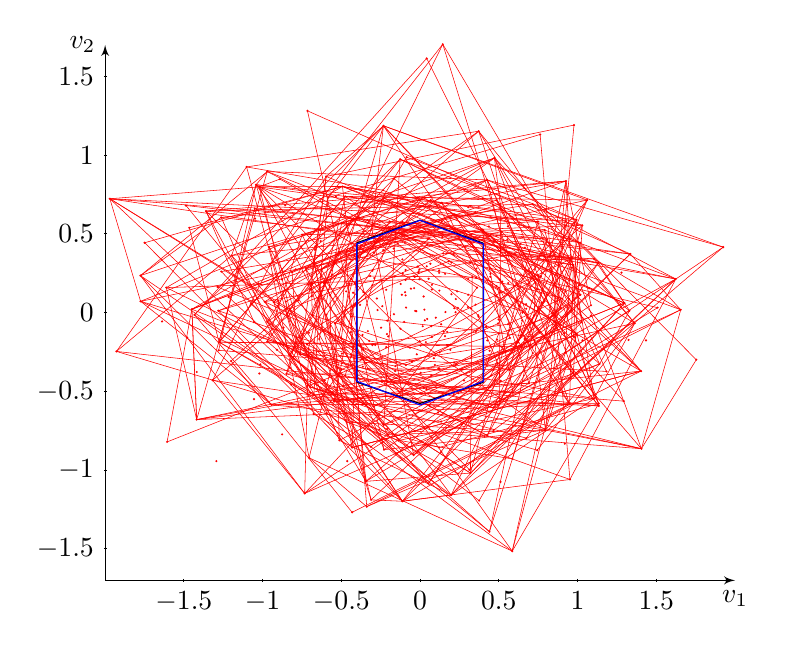
\begin{tikzpicture}[scale=2,rotate=0]
\draw[-latex'] (-2,-1.7) -- (2,-1.7) node[below] {$v_1$};
\foreach \x in {-1.5,-1,-0.5,0,0.5,1,1.5} \draw (\x,-1.69) -- (\x,-1.71) node[below] {$\x$};
\draw[-latex'] (-2,-1.7) -- (-2,1.7) node[left] {$v_2$};
\foreach \x in {-1.5,-1,-0.5,0,0.5,1,1.5} \draw (-1.99,\x) -- (-2.01,\x) node[left] {$\x$};
% \draw[very thin, gray] (-1.5,-.8) grid[step=.05] (2,.8);

\foreach \x/\y in { 0.80664/ 0.46653, -0.36815/-0.29486,  0.97678/-0.15217,  0.13819/ 0.57941,  0.02332/-0.47758, -0.19311/ 0.57889, -0.49765/ 0.57058, -0.11181/-0.48423, -0.63123/ 0.45473,  0.23500/ 0.13538, -1.04817/ 0.59720, -0.09274/ 0.20803,  0.94927/-0.58193,  0.30304/-0.66466, -1.35971/ 0.64501,  0.05414/ 0.21556, -0.71076/ 0.17700, -0.55756/ 0.24191, -0.61073/ 0.18745,  1.92499/ 0.41608, -0.33167/-0.11753, -1.07282/ 0.05467,  0.74794/ 0.57842, -0.44940/ 0.18379,  0.21665/ 0.02804, -0.49885/-0.36203,  0.00308/-0.20937, -0.30249/ 0.26601,  0.50516/-0.02779,  0.21962/ 0.62409, -0.41312/ 0.18531,  0.35414/-0.12223, -0.16635/-0.00980, -0.53425/ 0.73632,  0.00364/-0.38220, -0.22829/ 0.72890, -1.26210/ 0.26086,  0.60211/ 0.37265, -0.97069/ 0.89601, -0.21563/ 0.14493, -0.43784/-0.02433, -0.96998/-0.18264, -0.56823/-0.13665,  0.24048/ 0.03004,  0.67287/ 0.05367, -1.92819/-0.24617,  0.79045/ 0.52488,  1.40319/-0.37094,  0.94736/ 0.08529,  0.49990/ 0.15836,  0.30552/ 0.11345, -0.31105/-1.18889, -0.87617/-0.77297, -0.33866/-1.23193,  0.24688/ 0.48565, -1.05459/-0.06011, -0.36054/-0.23722,  0.56631/-0.11267, -0.40487/-0.55060,  0.07420/ 0.14650,  0.07516/ 0.17660,  0.51782/ 0.51399, -0.41668/ 0.04392,  0.32311/ 0.02659,  0.24261/-0.51127,  0.44134/-0.24208, -0.12685/ 0.97408, -0.05818/ 0.15225, -1.74889/ 0.44383,  1.13425/-0.57790, -0.15808/-0.37101, -1.41872/-0.67918, -0.03117/ 0.01052,  0.48867/-0.17120, -0.23555/ 0.77734, -0.51580/-0.40417,  0.35753/ 0.27938, -0.02389/ 0.00905, -0.48183/ 0.61210,  0.14677/ 0.37633,  0.79313/ 0.35496, -1.46574/ 0.53925, -0.38086/ 0.04899,  0.12044/-0.85598,  1.07402/ 0.15467,  0.49433/-0.06977,  0.36900/-0.01662, -0.19174/ 0.53194, -0.04638/-0.54648,  0.40177/-0.38601, -0.43469/-0.27524,  0.78898/ 0.07064, -0.78494/-0.16274,  0.41989/-0.08930, -0.34386/-1.07131, -0.84528/-0.00667, -1.27896/-0.23923, -0.36315/-0.34285, -0.66576/ 0.42166, -1.19683/ 0.36284, -0.21036/-0.13575,  0.44621/ 0.24589,  0.55767/ 0.54769,  0.48369/ 0.10327,  0.44064/-1.39092,  0.55946/ 0.18761,  0.66331/-0.16686,  0.04512/-0.04022, -1.04145/ 0.81222, -1.44945/ 0.02168, -0.52963/ 0.37057,  0.05257/-1.08593,  0.97363/-0.37702, -1.02078/-0.38636,  0.42717/-0.17641, -1.96982/ 0.72320, -0.23835/ 0.49551,  0.76663/ 0.23072,  0.06820/ 0.71467, -1.01479/-0.32886, -0.90967/-0.23575, -1.05003/ 0.66113,  0.12076/ 0.26827,  0.42521/ 0.84289, -0.46564/-0.69450, -0.78956/ 0.27450,  0.12228/ 0.13983,  0.15803/-0.14887, -1.21656/ 0.09938,  1.13442/-0.59228,  0.71469/ 0.68870, -0.59457/-0.01331,  0.18542/ 0.54974,  0.77452/ 0.06427,  0.09621/-0.27148,  0.13423/-0.88407,  0.37199/ 1.15196,  0.79617/-0.74555,  0.91879/-0.83207,  0.89673/ 0.02781, -1.05476/-0.54933,  0.14146/ 0.48055, -0.54642/-0.56319, -0.47140/ 0.36921,  0.63242/ 0.03911,  1.02588/-0.05983,  0.44258/-0.47319,  0.19883/ 0.11717, -0.32301/-0.17979,  0.46761/ 0.45278, -0.82763/-0.26958,  0.97330/ 0.30288,  1.43427/-0.17611, -0.12485/-0.10211, -0.11245/ 0.57626,  0.95159/-1.05927, -0.46961/ 0.13520, -0.50060/-0.16365, -0.06396/-0.22273, -1.28101/ 0.01193, -0.69541/ 0.15038, -1.77493/ 0.07188, -0.12317/ 0.18201, -0.37683/-0.54624, -0.11556/ 0.11360, -0.63167/-0.54749, -0.31233/-0.85168, -1.29344/-0.94295,  0.22662/ 0.08642,  0.04181/ 1.61447,  0.31864/ 0.31791, -0.13459/-0.81144,  0.92583/ 0.58251,  0.31961/-1.01862,  0.48564/ 0.16825,  1.50824/ 0.03170, -0.48910/-0.46916, -0.21489/-0.21892,  0.76207/ 1.13141, -0.86714/-0.09504, -0.15054/-0.89351,  0.12404/-0.25225, -0.43221/ 0.59093,  0.46631/-0.36361,  0.61347/-0.18480, -0.43785/-0.00784, -0.71783/-0.20258, -0.36541/-0.14147, -0.08546/ 0.98685,  0.54558/-0.24549,  0.66542/ 0.41176,  0.67437/ 0.02478, -0.94971/ 0.31028,  0.25774/-0.49858,  1.32388/-0.17324,  0.59027/-0.50807,  0.99506/-0.13488, -0.37538/ 0.42539, -0.16562/ 0.85144,  1.29775/ 0.06066,  1.75374/-0.29886, -0.59196/-0.63809, -0.87750/ 0.21083, -0.29153/ 0.38038,  0.21618/-0.31628, -0.31473/-0.42823,  0.14840/-0.11944,  0.58498/-1.51423,  1.29353/-0.56205,  0.58573/-0.92864,  0.46691/-0.60370,  1.65512/ 0.01818,  0.07052/-0.39737, -0.27020/ 0.01661,  0.01683/-0.08670, -0.94296/-0.58516,  0.30552/ 0.21402, -0.59630/ 0.86480,  0.01715/ 0.73180, -0.49286/ 0.80118,  0.18218/ 0.32710, -0.90209/ 0.04226,  1.32967/ 0.01199,  0.05785/ 0.47063,  0.49836/-0.04371,  0.21164/ 0.36985,  0.00436/-0.51027,  0.80562/ 0.11382,  0.04896/ 0.56860, -1.26285/ 0.60466,  0.12074/ 0.25260,  0.67502/-0.79688,  1.36272/-0.06730, -1.60651/-0.82076,  0.89995/ 0.09005, -0.03813/ 0.15565, -0.69015/ 0.18251, -0.36073/ 0.13078,  1.13172/ 0.31573,  0.99286/ 0.58913,  0.07092/-0.08534,  0.50269/-0.58396, -0.09183/ 0.27081,  0.39369/-0.30424,  0.16112/ 0.00379, -0.81786/-0.45845, -0.30669/ 0.53414,  0.51266/ 0.66216,  0.62263/ 0.16806,  0.02242/ 0.10293,  0.92427/ 0.13430,  0.72413/-0.01688, -1.47841/-0.15803,  0.09400/-0.33251, -0.03306/-0.75212, -0.47611/-0.40020, -0.16137/ 0.23007,  0.40053/ 0.52333,  0.71315/-0.21781,  1.08523/ 0.04667, -0.69887/-0.47151, -0.67601/-0.64323,  0.91633/-0.13140,  0.71595/-0.25675,  1.01021/ 0.17362, -0.66787/ 0.39893,  0.42699/-0.77972, -0.98691/ 0.06935, -0.49649/-0.26024,  0.54031/ 0.14927,  0.74439/ 0.14789,  1.03146/-0.17609,  0.09989/-0.03190,  0.09389/-0.54583,  0.49176/-0.31939, -0.71533/ 1.28149, -0.73292/-1.14809, -0.20624/-0.43922,  1.27885/ 0.25410,  0.19513/-0.20238, -0.04124/-0.90466, -0.46500/ 0.55041, -0.84872/-0.38874,  0.36150/ 0.15898,  0.55412/ 0.46522, -0.23293/ 1.18655, -0.09678/ 0.44302, -0.09542/ 0.12969, -1.02767/ 0.18602, -0.20921/-0.73852,  0.19710/-1.15804,  0.27191/ 0.50844, -0.43705/ 0.21427,  0.22464/-0.33355,  0.06100/-0.59262,  0.48591/ 0.48825, -0.02064/-0.26454,  1.40536/-0.86399,  1.01613/ 0.44442,  0.79683/ 0.65476, -1.77586/ 0.23521,  0.02741/ 0.01914, -0.51239/-0.81116, -0.68338/ 0.18623,  0.04220/ 0.29458,  0.55279/-0.55553, -0.01058/ 0.25241, -0.58410/ 0.73053,  0.62115/-0.18930,  0.06516/ 0.31042, -0.46278/-0.94301,  0.30371/ 0.03530, -0.85595/ 0.68224,  0.37064/-0.02542,  0.40280/ 0.04940, -0.43164/-0.85677, -0.30307/ 0.17362, -0.69646/-0.50878,  0.95680/ 0.34093,  0.51060/-1.07428, -0.38958/ 0.60666,  0.23984/-1.02229,  0.62764/ 0.04467,  0.74429/-0.87324,  0.64049/-0.21347,  0.31328/-0.99812,  0.37485/-1.19341,  0.22522/ 0.00283,  0.04503/ 0.43051, -0.28433/-0.20502,  0.13790/ 0.69707, -0.33075/-0.35625, -1.02161/ 0.79879,  0.50681/ 0.20948,  1.01810/ 0.11345, -0.48433/-0.18598,  0.47199/ 0.98197,  0.50014/-0.13061, -0.00456/ 0.21170, -0.20526/-0.77339, -0.52546/-0.35054, -0.76202/-0.26325,  0.04022/-0.48522, -0.21120/ 0.43665,  0.35445/ 0.22328, -0.11014/ 0.25024, -0.50037/-0.06297, -1.61148/ 0.15897, -1.41840/-0.37669,  0.92604/ 0.83569,  1.10527/-0.54542, -0.53986/-0.06901,  0.02975/-0.04874,  0.54906/ 0.00569,  0.73303/ 0.18760,  0.19177/-0.23584,  0.32235/ 0.44738,  0.96200/ 0.28566, -1.10181/ 0.92519, -0.39295/ 0.35252, -0.82473/-0.35189, -0.23877/ 0.15304, -0.74887/ 0.49515, -1.43271/-0.01392,  0.07477/-0.15431, -1.28665/ 0.16327, -0.67568/ 0.32817, -0.16785/ 0.40695,  0.50659/ 0.12985,  0.17213/-0.12233,  0.49369/-0.44950, -0.10137/-0.05835, -0.30236/-0.20585, -0.39324/ 0.26952,  1.02994/ 0.55454, -0.92850/ 0.06579,  0.27874/-0.43032, -0.11246/ 0.33854, -0.68457/-0.01577,  0.64905/-0.04937,  0.74931/ 0.23213, -0.47604/ 0.73807,  0.13414/-0.69170, -0.55499/-0.50824, -1.63820/-0.05569,  0.15837/ 0.24673,  0.33092/ 0.22566, -0.54319/-0.55305,  0.23236/-0.32697,  0.08785/-0.28959, -0.16802/ 0.53255, -0.43150/-1.26788, -0.27418/ 0.08976,  0.78931/-0.16196, -0.00946/ 0.26185,  0.43609/ 0.54732, -0.62554/ 0.27450, -0.41038/ 0.05240,  0.92187/-0.25269,  1.08420/-0.02082, -0.40828/ 0.34249, -0.70876/-0.22718, -0.24471/-0.43637,  0.44632/ 0.48801, -0.46557/ 0.39159, -0.72549/ 0.27796, -0.60605/-0.43115,  0.73669/-0.20404, -0.82903/ 0.02375, -0.70484/-0.92191, -0.22861/-0.87034, -0.11231/-1.19762, -0.54354/-0.17637, -0.23963/ 0.04098, -0.85266/ 0.07043,  0.12272/-0.35459,  0.65416/ 0.00695, -1.31774/-0.42926, -0.42497/ 0.12630, -0.57123/ 0.11025,  0.57059/-0.16058, -0.90000/ 0.07524,  0.26540/-0.71017,  0.85006/-0.02045, -0.49279/-0.22965,  0.65037/ 0.00025, -0.09007/-0.33334,  0.21422/-0.51675,  0.14406/ 1.70440, -0.05127/-0.31127,  0.56894/-0.36340, -0.43942/-0.12336, -0.09161/ 0.10973,  0.35260/ 0.05103, -0.64048/-0.16721, -0.20203/-0.15051,  0.97725/ 1.19101, -0.42971/ 0.03641,  0.30596/ 0.66933,  0.13320/-0.07375,  0.31399/-0.66630,  0.17362/-0.20886, -1.20024/-0.30739, -0.20866/-0.05051, -0.44072/ 0.33770,  0.11351/-0.63405, -0.95929/ 0.41780,  0.44998/-0.39904, -0.70582/-0.12772, -0.08915/ 0.03199,  1.06120/ 0.71492, -0.51543/ 0.38535,  0.63911/ 0.43631,  0.44580/ 0.22731, -0.24148/-0.32471,  0.19852/ 0.31789,  0.46684/-0.74582, -0.31732/ 0.23264, -0.00334/-0.18147, -0.16440/-0.44572,  0.75736/-0.12489, -0.77315/ 0.07737, -0.68722/ 0.10605, -0.14192/ 0.43867, -0.97052/-0.05864,  0.17131/-0.39188, -0.00415/ 0.27330, -0.81272/ 0.25625,  0.96076/ 0.01798, -1.27628/-0.18730,  1.18333/-0.37332,  0.72667/-0.17795, -0.56780/ 0.02744, -0.23404/ 0.39721, -0.23074/-0.71227, -0.29586/-0.59630,  1.10417/ 0.34135,  0.39365/ 0.52921,  0.03672/-0.18692, -1.48687/ 0.68036, -0.29062/ 0.21964, -0.03359/ 0.22696, -0.15671/-0.33963,  0.48409/ 0.71415, -0.88997/ 0.84808,  1.33489/ 0.37273,  0.69091/-0.44850,  0.52138/ 0.19694,  0.92537/ 0.55380, -0.01392/ 0.29307,  0.51254/-0.43293,  0.55869/-0.07335,  0.04838/ 0.46612,  0.35000/ 0.63917, -0.43841/-0.26497, -0.24759/-0.09559,  0.11582/-0.35347,  1.62375/ 0.21381,  1.13972/-0.32561, -0.67412/-0.51928}
 \fill[red] (\x,\y) circle (.05ex);

\draw[very thin, red] (  1.1833,  -0.3733) -- (  0.8066,   0.4665) -- (  0.4859,   0.4883) -- ( -0.4656,   0.3916) -- ( -0.5154,   0.3854) -- ( -1.2621,   0.2609) -- ( -0.7620,  -0.2632) -- (  1.1833,  -0.3733) -- cycle;
\draw[very thin, red] (  1.1317,   0.3157) -- ( -0.1917,   0.5319) -- ( -1.3177,  -0.4293) -- ( -0.7329,  -1.1481) -- (  1.1397,  -0.3256) -- (  1.3297,   0.0120) -- (  1.1317,   0.3157) -- cycle;
\draw[very thin, red] (  0.6909,  -0.4485) -- (  0.9568,   0.3409) -- ( -0.4322,   0.5909) -- ( -1.1968,   0.3628) -- ( -0.3439,  -1.0713) -- (  0.6909,  -0.4485) -- cycle;
\draw[very thin, red] ( -0.2286,  -0.8703) -- (  0.7893,  -0.1620) -- (  1.3349,   0.3727) -- ( -0.7153,   1.2815) -- ( -0.2286,  -0.8703) -- cycle;
\draw[very thin, red] (  1.4032,  -0.3709) -- (  0.5178,   0.5140) -- (  0.2196,   0.6241) -- ( -1.2810,   0.0119) -- ( -0.4316,  -0.8568) -- (  1.4032,  -0.3709) -- cycle;
\draw[very thin, red] (  0.4426,  -0.4732) -- (  0.7745,   0.0643) -- (  0.3937,   0.5292) -- ( -0.2329,   1.1865) -- ( -0.3067,   0.5341) -- ( -0.0412,  -0.9047) -- (  0.4426,  -0.4732) -- cycle;
\draw[very thin, red] ( -0.4760,   0.7381) -- ( -1.2763,  -0.1873) -- ( -0.6317,  -0.5475) -- (  0.5027,  -0.5840) -- (  1.0612,   0.7149) -- ( -0.4760,   0.7381) -- cycle;
\draw[very thin, red] ( -0.5006,  -0.1636) -- ( -0.1118,  -0.4842) -- (  0.6909,  -0.4485) -- (  0.4856,   0.1683) -- ( -0.2283,   0.7289) -- ( -0.4494,   0.1838) -- ( -0.5006,  -0.1636) -- cycle;
\draw[very thin, red] ( -0.4049,  -0.5506) -- (  0.3196,  -1.0186) -- (  1.6237,   0.2138) -- (  0.7147,   0.6887) -- ( -0.9593,   0.4178) -- ( -0.4049,  -0.5506) -- cycle;
\draw[very thin, red] ( -0.3929,   0.3525) -- ( -0.4394,  -0.1234) -- ( -0.3439,  -1.0713) -- (  0.3196,  -1.0186) -- (  0.7479,   0.5784) -- ( -0.1680,   0.5326) -- ( -0.3929,   0.3525) -- cycle;
\draw[very thin, red] ( -0.7048,  -0.9219) -- ( -0.3387,  -1.2319) -- (  0.7962,  -0.7455) -- (  0.7267,  -0.1779) -- (  0.1441,   1.7044) -- ( -0.9497,   0.3103) -- ( -0.7048,  -0.9219) -- cycle;
\draw[very thin, red] ( -0.4929,   0.8012) -- ( -1.7489,   0.4438) -- ( -0.1123,  -1.1976) -- (  0.1971,  -1.1580) -- (  1.2977,   0.0607) -- ( -0.4929,   0.8012) -- cycle;
\draw[very thin, red] (  1.1042,   0.3414) -- (  0.6021,   0.3727) -- ( -0.9869,   0.0693) -- ( -0.1505,  -0.8935) -- (  1.6551,   0.0182) -- (  1.1042,   0.3414) -- cycle;
\draw[very thin, red] ( -0.4378,  -0.0243) -- (  0.7893,  -0.1620) -- (  0.9254,   0.5538) -- ( -1.0414,   0.8122) -- ( -0.4378,  -0.0243) -- cycle;
\draw[very thin, red] ( -0.6965,  -0.5088) -- (  1.3627,  -0.0673) -- (  0.0682,   0.7147) -- ( -0.2384,   0.4955) -- ( -0.8276,  -0.2696) -- ( -0.6965,  -0.5088) -- cycle;
\draw[very thin, red] (  0.0172,   0.7318) -- ( -0.9593,   0.4178) -- ( -0.7849,  -0.1627) -- ( -0.5158,  -0.4042) -- (  0.5903,  -0.5081) -- (  0.3937,   0.5292) -- (  0.0172,   0.7318) -- cycle;
\draw[very thin, red] ( -0.7620,  -0.2632) -- (  0.5528,  -0.5555) -- (  0.9493,  -0.5819) -- ( -0.2329,   1.1865) -- ( -0.5963,   0.8648) -- ( -0.7620,  -0.2632) -- cycle;
\draw[very thin, red] (  1.0612,   0.7149) -- ( -0.2329,   1.1865) -- ( -0.4656,   0.3916) -- ( -0.5004,  -0.0630) -- ( -0.3230,  -0.1798) -- ( -0.0640,  -0.2227) -- (  0.3541,  -0.1222) -- (  1.0612,   0.7149) -- cycle;
\draw[very thin, red] ( -0.4322,   0.5909) -- ( -0.9700,  -0.1826) -- ( -0.1567,  -0.3396) -- (  0.8501,  -0.0204) -- (  0.9260,   0.8357) -- ( -0.4322,   0.5909) -- cycle;
\draw[very thin, red] (  0.5689,  -0.3634) -- (  1.6237,   0.2138) -- (  0.7931,   0.3550) -- (  0.1468,   0.3763) -- ( -0.6902,   0.1825) -- ( -0.6846,  -0.0158) -- (  0.0962,  -0.2715) -- (  0.5689,  -0.3634) -- cycle;
\draw[very thin, red] (  0.4841,   0.7141) -- ( -0.4714,   0.3692) -- ( -0.3387,  -1.2319) -- (  1.4032,  -0.3709) -- (  0.4841,   0.7141) -- cycle;
\draw[very thin, red] (  0.1971,  -1.1580) -- (  1.6237,   0.2138) -- (  0.7904,   0.5249) -- ( -0.7489,   0.4952) -- ( -0.9700,  -0.1826) -- ( -0.1505,  -0.8935) -- (  0.1971,  -1.1580) -- cycle;
\draw[very thin, red] (  1.0852,   0.0467) -- (  0.9260,   0.8357) -- ( -1.2628,   0.6047) -- ( -1.7759,   0.2352) -- ( -0.7329,  -1.1481) -- (  1.0852,   0.0467) -- cycle;
\draw[very thin, red] (  0.4669,  -0.6037) -- (  0.9608,   0.0180) -- (  1.0161,   0.4444) -- (  0.5178,   0.5140) -- ( -0.7896,   0.2745) -- ( -1.7749,   0.0719) -- (  0.4669,  -0.6037) -- cycle;
\draw[very thin, red] (  0.5850,  -1.5142) -- (  1.1343,  -0.5779) -- (  0.4252,   0.8429) -- ( -0.7489,   0.4952) -- ( -0.5712,   0.1103) -- (  0.5850,  -1.5142) -- cycle;
\draw[very thin, red] (  1.2977,   0.0607) -- ( -0.2283,   0.7289) -- ( -1.4494,   0.0217) -- ( -1.4187,  -0.6792) -- (  0.3937,  -0.3042) -- (  1.2977,   0.0607) -- cycle;
\draw[very thin, red] ( -0.5550,  -0.5082) -- (  0.5027,  -0.5840) -- (  0.5127,   0.6622) -- (  0.4720,   0.9820) -- ( -1.7749,   0.0719) -- ( -0.5550,  -0.5082) -- cycle;
\draw[very thin, red] (  1.0299,   0.5545) -- ( -0.4929,   0.8012) -- ( -1.4657,   0.5392) -- ( -1.2763,  -0.1873) -- (  0.1951,  -0.2024) -- (  1.0299,   0.5545) -- cycle;
\draw[very thin, red] ( -0.7255,   0.2780) -- ( -0.3682,  -0.2949) -- (  0.3133,  -0.9981) -- (  1.2977,   0.0607) -- (  0.1854,   0.5497) -- ( -0.7255,   0.2780) -- cycle;
\draw[very thin, red] (  0.9493,  -0.5819) -- (  0.3720,   1.1520) -- ( -0.6255,   0.2745) -- ( -0.6741,  -0.5193) -- ( -0.1123,  -1.1976) -- (  0.9493,  -0.5819) -- cycle;
\draw[very thin, red] (  0.1379,   0.6971) -- ( -1.0414,   0.8122) -- ( -1.2790,  -0.2392) -- ( -0.2415,  -0.3247) -- (  0.6212,  -0.1893) -- (  0.9929,   0.5891) -- (  0.1379,   0.6971) -- cycle;
\draw[very thin, red] (  1.4054,  -0.8640) -- (  1.6551,   0.0182) -- ( -0.4929,   0.8012) -- ( -1.0216,   0.7988) -- ( -0.1248,  -0.1021) -- (  0.7962,  -0.7455) -- (  1.4054,  -0.8640) -- cycle;
\draw[very thin, red] (  1.1343,  -0.5779) -- (  0.7931,   0.3550) -- ( -0.2356,   0.7773) -- ( -1.1018,   0.9252) -- ( -1.9282,  -0.2462) -- (  0.1204,  -0.8560) -- (  1.1343,  -0.5779) -- cycle;
\draw[very thin, red] ( -0.7178,  -0.2026) -- (  0.4270,  -0.7797) -- (  0.7159,  -0.2567) -- (  0.4999,   0.1584) -- (  0.0578,   0.4706) -- ( -0.7178,  -0.2026) -- cycle;
\draw[very thin, red] (  0.7443,  -0.8732) -- (  1.3627,  -0.0673) -- (  0.3720,   1.1520) -- ( -0.6658,   0.4217) -- ( -0.9705,  -0.0586) -- ( -0.6989,  -0.4715) -- (  0.7443,  -0.8732) -- cycle;
\draw[very thin, red] ( -0.6760,  -0.6432) -- ( -0.3123,  -0.8517) -- (  1.0181,   0.1135) -- (  0.3720,   1.1520) -- ( -1.1018,   0.9252) -- ( -0.6760,  -0.6432) -- cycle;
\draw[very thin, red] ( -0.7849,  -0.1627) -- ( -0.8487,  -0.3887) -- (  0.1713,  -0.3919) -- (  1.2977,   0.0607) -- (  1.1042,   0.3414) -- (  0.1822,   0.3271) -- ( -0.2388,   0.1530) -- ( -0.7849,  -0.1627) -- cycle;
\draw[very thin, red] (  1.1053,  -0.5454) -- (  1.3627,  -0.0673) -- (  0.7147,   0.6887) -- ( -1.3597,   0.6450) -- ( -0.4384,  -0.2650) -- (  1.1053,  -0.5454) -- cycle;
\draw[very thin, red] (  0.9772,   1.1910) -- ( -0.5963,   0.8648) -- ( -0.9497,   0.3103) -- ( -1.3177,  -0.4293) -- (  0.7962,  -0.7455) -- (  0.9772,   1.1910) -- cycle;
\draw[very thin, red] (  0.9768,  -0.1522) -- (  0.9929,   0.5891) -- ( -0.0855,   0.9869) -- ( -0.8276,  -0.2696) -- (  0.3749,  -1.1934) -- (  0.9768,  -0.1522) -- cycle;
\draw[very thin, red] (  0.9733,   0.3029) -- (  0.0450,   0.4305) -- ( -0.5399,  -0.0690) -- ( -0.5124,  -0.8112) -- (  0.1971,  -1.1580) -- (  1.1053,  -0.5454) -- (  0.9733,   0.3029) -- cycle;
\draw[very thin, red] (  1.9250,   0.4161) -- (  0.4252,   0.8429) -- ( -0.9707,   0.8960) -- ( -1.0414,   0.8122) -- ( -0.6317,  -0.5475) -- (  0.2398,  -1.0223) -- (  1.9250,   0.4161) -- cycle;
\draw[very thin, red] (  0.3223,   0.4474) -- ( -0.1124,   0.5763) -- ( -1.4494,   0.0217) -- ( -0.3147,  -0.4282) -- (  1.1344,  -0.5923) -- (  0.3223,   0.4474) -- cycle;
\draw[very thin, red] ( -0.1931,   0.5789) -- ( -0.5946,  -0.0133) -- ( -0.3110,  -1.1889) -- ( -0.1123,  -1.1976) -- (  0.9516,  -1.0593) -- (  1.6237,   0.2138) -- ( -0.1931,   0.5789) -- cycle;
\draw[very thin, red] ( -0.4891,  -0.4692) -- (  1.4054,  -0.8640) -- (  1.7537,  -0.2989) -- (  1.0161,   0.4444) -- ( -0.1268,   0.9741) -- ( -1.0728,   0.0547) -- ( -0.4891,  -0.4692) -- cycle;
\draw[very thin, red] (  0.4426,  -0.4732) -- (  1.4032,  -0.3709) -- ( -0.1680,   0.5326) -- ( -1.3597,   0.6450) -- ( -1.0546,  -0.0601) -- ( -0.3768,  -0.5462) -- (  0.4426,  -0.4732) -- cycle;
\draw[very thin, red] (  1.1053,  -0.5454) -- (  0.9951,  -0.1349) -- ( -0.2329,   1.1865) -- ( -1.4327,  -0.0139) -- ( -0.4656,  -0.6945) -- ( -0.1346,  -0.8114) -- (  1.1053,  -0.5454) -- cycle;
\draw[very thin, red] (  0.9733,   0.3029) -- (  0.1441,   1.7044) -- ( -0.8276,  -0.2696) -- (  0.4406,  -1.3909) -- (  0.9733,   0.3029) -- cycle;
\draw[very thin, red] (  0.5850,  -1.5142) -- (  0.9474,   0.0853) -- (  0.9243,   0.1343) -- (  0.1854,   0.5497) -- ( -0.3754,   0.4254) -- ( -0.7048,  -0.9219) -- (  0.5850,  -1.5142) -- cycle;
\draw[very thin, red] (  0.9608,   0.0180) -- (  1.0161,   0.4444) -- (  0.3500,   0.6392) -- ( -0.4760,   0.7381) -- ( -1.2763,  -0.1873) -- (  0.7131,  -0.2178) -- (  0.9608,   0.0180) -- cycle;
\draw[very thin, red] ( -1.7759,   0.2352) -- ( -0.6741,  -0.5193) -- (  0.2426,  -0.5113) -- (  0.4426,  -0.4732) -- (  1.1317,   0.3157) -- (  0.4720,   0.9820) -- ( -1.7759,   0.2352) -- cycle;
\draw[very thin, red] (  0.0939,  -0.5458) -- (  1.1344,  -0.5923) -- (  0.6542,   0.0070) -- ( -0.0968,   0.4430) -- ( -1.9698,   0.7232) -- (  0.0939,  -0.5458) -- cycle;
\draw[very thin, red] ( -0.1917,   0.5319) -- ( -0.7255,   0.2780) -- ( -0.3439,  -1.0713) -- (  0.8967,   0.0278) -- (  0.4463,   0.4880) -- ( -0.1917,   0.5319) -- cycle;
\draw[very thin, red] ( -0.3173,   0.2326) -- ( -0.8290,   0.0238) -- ( -0.4049,  -0.5506) -- (  0.3196,  -1.0186) -- (  0.3309,   0.2257) -- ( -0.3173,   0.2326) -- cycle;
\draw[very thin, red] ( -0.5464,  -0.5632) -- (  0.0233,  -0.4776) -- (  0.4918,  -0.3194) -- (  0.3690,  -0.0166) -- ( -0.1419,   0.4387) -- ( -0.8527,   0.0704) -- ( -0.8453,  -0.0067) -- ( -0.5464,  -0.5632) -- cycle;
\draw[very thin, red] ( -1.0500,   0.6611) -- ( -1.2763,  -0.1873) -- ( -0.0412,  -0.9047) -- (  0.4500,  -0.3990) -- (  0.8066,   0.4665) -- ( -1.0500,   0.6611) -- cycle;
\draw[very thin, red] ( -0.9430,  -0.5852) -- (  1.1343,  -0.5779) -- (  0.0418,   1.6145) -- ( -1.4327,  -0.0139) -- ( -0.9430,  -0.5852) -- cycle;
\draw[very thin, red] ( -0.8290,   0.0238) -- ( -0.5124,  -0.8112) -- (  0.5456,  -0.2455) -- ( -0.4322,   0.5909) -- ( -0.8900,   0.8481) -- ( -1.0216,   0.7988) -- ( -0.8290,   0.0238) -- cycle;
\draw[very thin, red] ( -1.2002,  -0.3074) -- ( -0.4315,  -1.2679) -- (  0.9493,  -0.5819) -- (  0.9733,   0.3029) -- ( -0.3067,   0.5341) -- ( -1.2002,  -0.3074) -- cycle;
\draw[very thin, red] (  0.4720,   0.9820) -- (  0.0172,   0.7318) -- ( -0.5399,  -0.0690) -- ( -0.2286,  -0.8703) -- (  0.7962,  -0.7455) -- (  1.1397,  -0.3256) -- (  0.4720,   0.9820) -- cycle;
\draw[very thin, red] (  0.9929,   0.5891) -- (  0.4252,   0.8429) -- ( -1.2867,   0.1633) -- ( -0.0901,  -0.3333) -- (  0.4943,  -0.0698) -- (  0.9929,   0.5891) -- cycle;
\draw[very thin, red] ( -1.4869,   0.6804) -- ( -0.9869,   0.0693) -- (  0.2426,  -0.5113) -- (  0.5903,  -0.5081) -- (  1.1317,   0.3157) -- (  0.6391,   0.4363) -- ( -1.4869,   0.6804) -- cycle;
\draw[very thin, red] (  0.9951,  -0.1349) -- (  0.3544,   0.2233) -- ( -0.9707,   0.8960) -- ( -1.7759,   0.2352) -- ( -0.9430,  -0.5852) -- (  0.2577,  -0.4986) -- (  0.9951,  -0.1349) -- cycle;
\draw[very thin, red] ( -1.4494,   0.0217) -- ( -1.6065,  -0.8208) -- (  0.0748,  -0.1543) -- (  0.7666,   0.2307) -- (  1.0612,   0.7149) -- ( -0.5296,   0.3706) -- ( -1.4494,   0.0217) -- cycle;
\draw[very thin, red] (  0.1379,   0.6971) -- ( -0.4929,   0.8012) -- ( -0.4650,   0.5504) -- ( -0.2062,  -0.4392) -- (  1.2935,  -0.5620) -- (  0.1379,   0.6971) -- cycle;
\draw[very thin, red] ( -1.3597,   0.6450) -- ( -0.8247,  -0.3519) -- (  0.4406,  -1.3909) -- (  0.9260,   0.8357) -- ( -1.3597,   0.6450) -- cycle;
\draw[very thin, red] ( -1.4187,  -0.6792) -- ( -0.3768,  -0.5462) -- (  0.5491,   0.0057) -- (  0.7666,   0.2307) -- (  0.8066,   0.4665) -- (  0.7904,   0.5249) -- ( -0.4929,   0.8012) -- ( -1.6115,   0.1590) -- ( -1.4187,  -0.6792) -- cycle;
\draw[very thin, red] ( -0.6989,  -0.4715) -- ( -0.2959,  -0.5963) -- (  0.6405,  -0.2135) -- (  1.0181,   0.1135) -- ( -1.0216,   0.7988) -- ( -1.9698,   0.7232) -- ( -0.6989,  -0.4715) -- cycle;
\draw[very thin, red] (  0.7241,  -0.0169) -- (  0.7330,   0.1876) -- (  0.6021,   0.3727) -- ( -0.5963,   0.8648) -- ( -0.6902,   0.1825) -- ( -0.2062,  -0.4392) -- (  0.0610,  -0.5926) -- (  0.4270,  -0.7797) -- (  0.7241,  -0.0169) -- cycle;
\draw[very thin, red] ( -1.7749,   0.0719) -- ( -0.9430,  -0.5852) -- (  0.1341,  -0.6917) -- (  1.1397,  -0.3256) -- (  0.1854,   0.5497) -- ( -1.9698,   0.7232) -- ( -1.7749,   0.0719) -- cycle;
\draw[very thin, red] ( -0.0046,   0.2117) -- ( -1.6115,   0.1590) -- ( -0.4761,  -0.4002) -- (  1.4054,  -0.8640) -- (  0.6542,   0.0070) -- ( -0.0046,   0.2117) -- cycle;
\draw[very thin, red] (  0.1379,   0.6971) -- ( -0.6255,   0.2745) -- ( -0.3605,  -0.2372) -- ( -0.1581,  -0.3710) -- (  0.2246,  -0.3335) -- (  0.5706,  -0.1606) -- (  0.1379,   0.6971) -- cycle;
\draw[very thin, red] (  0.9568,   0.3409) -- (  0.9260,   0.8357) -- ( -1.2166,   0.0994) -- (  0.0526,  -1.0859) -- (  0.9568,   0.3409) -- cycle;
\draw[very thin, red] (  0.9608,   0.0180) -- (  0.4005,   0.5233) -- ( -1.2810,   0.0119) -- (  0.2577,  -0.4986) -- (  0.9608,   0.0180) -- cycle;
\draw[very thin, red] ( -0.2329,   1.1865) -- ( -0.5841,   0.7305) -- ( -0.6757,   0.3282) -- ( -0.5158,  -0.4042) -- ( -0.0412,  -0.9047) -- (  1.9250,   0.4161) -- ( -0.2329,   1.1865) -- cycle;
\draw[very thin, red] (  1.3349,   0.3727) -- ( -0.1124,   0.5763) -- ( -0.3932,   0.2695) -- ( -0.4316,  -0.8568) -- ( -0.0331,  -0.7521) -- (  1.6551,   0.0182) -- (  1.3349,   0.3727) -- cycle;
\draw[very thin, red] ( -0.3123,  -0.8517) -- (  0.5850,  -1.5142) -- (  0.9219,  -0.2527) -- (  0.9568,   0.3409) -- ( -0.4988,  -0.3620) -- ( -0.6317,  -0.5475) -- ( -0.5920,  -0.6381) -- ( -0.3123,  -0.8517) -- cycle;
\draw[very thin, red] (  0.4937,  -0.4495) -- (  0.9219,  -0.2527) -- (  1.3297,   0.0120) -- (  0.5127,   0.6622) -- ( -0.1268,   0.9741) -- ( -0.2307,  -0.7123) -- (  0.4937,  -0.4495) -- cycle;
\draw[very thin, red] ( -0.9869,   0.0693) -- ( -0.7620,  -0.2632) -- (  0.5587,  -0.0733) -- (  0.9000,   0.0901) -- (  0.6226,   0.1681) -- ( -0.4714,   0.3692) -- ( -0.9869,   0.0693) -- cycle;
\draw[very thin, red] ( -0.6846,  -0.0158) -- ( -0.2959,  -0.5963) -- (  0.8967,   0.0278) -- (  0.7479,   0.5784) -- (  0.2196,   0.6241) -- ( -0.5154,   0.3854) -- ( -0.6846,  -0.0158) -- cycle;
\draw[very thin, red] (  1.5082,   0.0317) -- ( -0.2112,   0.4367) -- ( -0.6255,   0.2745) -- ( -0.8453,  -0.0067) -- ( -0.7620,  -0.2632) -- (  0.4669,  -0.6037) -- (  1.5082,   0.0317) -- cycle;
\draw[very thin, red] ( -0.4761,  -0.4002) -- ( -0.1346,  -0.8114) -- (  0.5857,  -0.9286) -- (  1.0299,   0.5545) -- (  0.3937,   0.5292) -- ( -0.2112,   0.4367) -- ( -0.3031,   0.1736) -- ( -0.4761,  -0.4002) -- cycle;
\draw[very thin, red] ( -0.8487,  -0.3887) -- (  0.6750,  -0.7969) -- (  0.9736,  -0.3770) -- (  1.0299,   0.5545) -- ( -0.1268,   0.9741) -- ( -0.4322,   0.5909) -- ( -0.8487,  -0.3887) -- cycle;
\draw[very thin, red] (  0.9516,  -1.0593) -- (  0.7621,   1.1314) -- ( -0.5841,   0.7305) -- ( -0.6989,  -0.4715) -- (  0.9516,  -1.0593) -- cycle;
\draw[very thin, red] (  0.4841,   0.7141) -- (  0.0172,   0.7318) -- ( -0.3754,   0.4254) -- ( -0.5712,   0.1103) -- ( -0.5682,  -0.1367) -- (  0.1971,  -1.1580) -- (  0.7890,   0.0706) -- (  0.4841,   0.7141) -- cycle;
\draw[very thin, red] (  1.4032,  -0.3709) -- (  0.9000,   0.0901) -- ( -0.3896,   0.6067) -- ( -0.4650,   0.5504) -- ( -0.6757,   0.3282) -- ( -0.4316,  -0.8568) -- (  1.4032,  -0.3709) -- cycle;
\draw[very thin, red] (  0.5001,  -0.1306) -- ( -1.0414,   0.8122) -- ( -1.1968,   0.3628) -- ( -0.2307,  -0.7123) -- (  0.4018,  -0.3860) -- (  0.5001,  -0.1306) -- cycle;
\draw[very thin, red] ( -0.8276,  -0.2696) -- ( -0.2053,  -0.7734) -- (  0.7962,  -0.7455) -- (  0.9951,  -0.1349) -- ( -0.1656,   0.8514) -- ( -0.9285,   0.0658) -- ( -0.8276,  -0.2696) -- cycle;
\draw[very thin, red] ( -1.4187,  -0.6792) -- (  0.9493,  -0.5819) -- (  0.5068,   0.2095) -- (  0.0490,   0.5686) -- ( -0.4656,   0.3916) -- ( -1.4494,   0.0217) -- ( -1.4187,  -0.6792) -- cycle;
\draw[very thin, red] ( -0.6405,  -0.1672) -- ( -0.3110,  -1.1889) -- (  1.3349,   0.3727) -- ( -0.4977,   0.5706) -- ( -0.6405,  -0.1672) -- cycle;
\draw[very thin, red] ( -0.9707,   0.8960) -- ( -1.4187,  -0.6792) -- (  0.1713,  -0.3919) -- (  0.6212,  -0.1893) -- (  0.7666,   0.2307) -- ( -0.9707,   0.8960) -- cycle;
\draw[very thin, red] ( -0.6107,   0.1875) -- ( -0.3308,  -0.3563) -- (  0.5689,  -0.3634) -- (  0.6491,  -0.0494) -- (  0.4252,   0.8429) -- ( -0.6107,   0.1875) -- cycle;
\draw[very thin, red] ( -0.1123,  -1.1976) -- (  0.3030,  -0.6647) -- (  0.9568,   0.3409) -- (  0.5127,   0.6622) -- (  0.0490,   0.5686) -- ( -0.8127,   0.2562) -- ( -0.7849,  -0.1627) -- ( -0.1123,  -1.1976) -- cycle;
\draw[very thin, red] ( -0.4297,   0.0364) -- ( -0.5432,  -0.5530) -- ( -0.1123,  -1.1976) -- (  1.0259,  -0.0598) -- (  0.4463,   0.4880) -- ( -0.3031,   0.1736) -- ( -0.4297,   0.0364) -- cycle;
\draw[very thin, red] ( -1.9698,   0.7232) -- (  0.0044,  -0.5103) -- (  1.0259,  -0.0598) -- (  0.9258,   0.5825) -- ( -1.9698,   0.7232) -- cycle;
\draw[very thin, red] (  1.4054,  -0.8640) -- (  0.9568,   0.3409) -- ( -1.2628,   0.6047) -- ( -0.9705,  -0.0586) -- ( -0.0331,  -0.7521) -- (  1.4054,  -0.8640) -- cycle;
\draw[very thin, red] ( -0.7329,  -1.1481) -- ( -0.1118,  -0.4842) -- (  0.3615,   0.1590) -- ( -0.4760,   0.7381) -- ( -0.7088,  -0.2272) -- ( -0.7329,  -1.1481) -- cycle;
\draw[very thin, red] ( -1.0216,   0.7988) -- ( -0.2053,  -0.7734) -- (  0.0526,  -1.0859) -- (  0.6405,  -0.2135) -- (  0.3223,   0.4474) -- (  0.2196,   0.6241) -- ( -1.0216,   0.7988) -- cycle;
\draw[very thin, red] ( -0.9705,  -0.0586) -- ( -0.4656,  -0.6945) -- (  0.4668,  -0.7458) -- (  0.9736,  -0.3770) -- (  0.4720,   0.9820) -- ( -0.9705,  -0.0586) -- cycle;
\draw[very thin, red] (  0.6405,  -0.2135) -- (  0.7574,  -0.1249) -- (  0.2719,   0.5084) -- ( -1.1968,   0.3628) -- ( -1.9282,  -0.2462) -- ( -0.2062,  -0.4392) -- (  0.1713,  -0.3919) -- (  0.6405,  -0.2135) -- cycle;




\draw (  0.4000,   0.4418) -- ( -0.0010,   0.5876) -- ( -0.4000,   0.4440) -- ( -0.4000,  -0.4423) -- ( -0.0012,  -0.5771) -- (  0.4000,  -0.4433) -- (  0.4000,   0.4418) -- cycle;

\draw[blue] (  0.4023,   0.4356) -- (  0.0000,   0.5864) -- ( -0.4023,   0.4356) -- ( -0.4023,  -0.4355) -- (  0.0000,  -0.5864) -- (  0.4023,  -0.4355) -- (  0.4023,   0.4356) -- cycle;


\end{tikzpicture}
\captionsetup{font=small}
\caption{Outlined in black the result~$\mathcal V$ of the optimisation~\eqref{seq:example:original}, the \textcolor{red}{red points} show samples drawn for this distribution and $100$~red outlined sets are convex hulls of a random selection of~$N=11$ samples such that any~$\textcolor{red}{\hat{\mathcal V}}$ allows statements on~\eqref{seq:example:original} to be made with a confidence larger than~$0.999$.
%
The result for the non-homogeneous grid discussed in Section~\ref{sec:improved:grid} is outlined in~\textcolor{blue}{blue}.}
\label{fig:example:in:comparison}
\end{figure}
%
%
%
\section{A Non-Homogeneous Grid}\label{sec:improved:grid}
%
%
%
\noindent In the previous section we presented a simple example using a homogeneous grid, this led to a large number of cubes~$Q_\bfa{i}$ and hence centre points~$c_\bfa{i}$.
%
Since the central approximation~\eqref{eq:central:approximation:formula} does not require a homogeneous grid and neither does Lemma~\ref{thm:sandwich:inequality}, we present in this section a method to determine a grid which reflects the properties of the probability density function more closely.
%
We consider a compact sample space~$\Omega\subseteq\mathcal B$ for some box~$\mathcal B=\{x\in\mathbb R^d:-\mathfrak{c}\leq x_i\leq \mathfrak{c}\}$.
%
The algorithm we suggest is to define a polytopal complex~$\mathcal C$ consisting of cubes~$Q_i$ such that~$\bigcup_{Q_i\in\mathcal C}Q_i=\mathcal B$ and the associated probability measure of each cube is below a certain threshold~$\mathfrak{f}_i\leq\mathfrak{f}_{\max}$.
%
To do this efficiently first notice that
\begin{multline*}
\int_0^{\delta}\dots\int_0^\delta \mathfrak{f}(t_1,\dots,t_d)\; \mathrm d t_1\dots \mathrm dt _d = \\ \delta^d\int_0^1\dots\int_0^1 \mathfrak {f}(\delta\tau_1,\dots,\delta\tau_d)
\; \mathrm d\tau_1\dots \mathrm d\tau_d .
\end{multline*}
Although this is a trivial substitution, it allows the simultaneous computation of~$\mathfrak{f}_i$ over differently sized cubes~$Q_i$.
%
Let~$\{q_1,\dots,q_{2^d}\}$ denote the vertices of the cube~$\mathcal Q=\{x\in\mathbb R^d: 0\leq x_i\leq 1\}$. For this algorithm it is convenient to characterise cubes by their \emph{lower left corner}~$b_i$ and their side length~$\delta_i$, so that the $i$th cube is given by~$Q_i=\conv_{1\leq k\leq2^d}\{b_i+\delta_i q_k\}$, and the associated measure is given by
\[
\mathfrak{f}_i=\int_{\mathcal Q}\mathfrak{f}(b_i+\delta_i\bfa{1} t) \; \mathrm d t.
\]
%
We propose the following algorithm to determine~$\mathcal C$:
%
\begin{algo}\label{algo:non:homo:cubes}
Choose desired~$\mathfrak{f}_{\max}>0$ and~$\delta_{\min}>0$, set~$\mathcal C=\mathcal B$ and evaluate~$\mathfrak{f}_i$\\
\textbf{WHILE} ($\max_i\{\mathfrak{f}_i\}\geq\mathfrak{f}_{\max}$~\textbf{AND}~$\min\{\delta_i\}\geq\delta_{\min}$) \textbf{DO} $\bigl($\\
$IDX := \mathfrak{f}_i\geq \mathfrak{f}_{\max}$\\
\textbf{FOR} $i\in IDX$ $\{$ \textbf{REPLACE} $b_i$ by $b_i+q_k$, $k\in\{1,\dots,2^d\}$ 
and $\delta_i$ by~$\frac{\delta_i}{2}\}$\\
\textbf{EVALUATE}~$\mathfrak f_i, i\in IDX\\
\textbf{UPDATE}~\mathcal C$
$\bigr)$
\end{algo}
%
Algorithm~\ref{algo:non:homo:cubes} terminates either when every cube contains a probability measure below the threshold $\mathfrak{f}_{\max}$ or when some cubes become smaller than the threshold $\delta_{\min}$. Otherwise it replaces all cubes for which the probability measure is larger than~$\mathfrak{f}_{\max}$ with cubes with a halved side length.
%
Once the grid is found the centre points are given by~$c_i=b_i+\frac{\delta_i}{2}\bfa{1}$.
%


%
Algorithm~\ref{algo:non:homo:cubes} can reduce the computational overhead significantly:
%
For the same example as in Section~\ref{sec:example} with a non-homogeneous grid satisfying~$\mathfrak{f}_i\leq\frac{1}{20000}$ which yields~$\min_i\{\delta_i\}=\frac{1}{2^7}=0.0078125$,~$\max_i\{\delta_i\}=\frac{1}{2}$ and a total of~$45436$ cubes.
%
Since~\eqref{eq:central:approximation:formula} does not depend on the choice of the grid itself the remaining optimisation is unchanged, a single evaluation of~$\mathring{P}(\mathcal V)$ now takes $0.0251$ seconds,
%~$0.025115$, 
i.e. about five times  faster than the homogeneous counterpart. The resulting set~$\mathcal V$ is shown in \textcolor{blue}{blue} in Figure~\ref{fig:example:in:comparison},
% and numerical values are reported in Table~\ref{tab:only:table}.
%
For illustrative purposes, Figure~\ref{fig:inhomogeneous:grid} shows a (slightly less fine) grid constructed using Algorithm~\ref{algo:non:homo:cubes}.

%
We summarise the numerical values of the proposed schemes in Table~\ref{tab:only:table}.
%
The first row of the table shows values for the homogeneous grid with~$160000$ cubes (with no direct influence on the measure of each box), the second row gives values for the inhomogeneous grid, while the third row shows the values obtained with the grid shown in Figure~\ref{fig:inhomogeneous:grid}. 
%
Both scenario based sets are evaluated on the inhomogeneous grid, with~$\underline{P}(\mathcal V)$ and~$\overline{P}(\mathcal V)$ evaluated at extreme values of the generated convex hulls, and the values of $\mathring{P}(\mathcal V)$ are the  arithmetic means of all $100$ sample sets.
%

%
%
%
%
%
\begin{figure}\centering
\ifodd0
\begin{tikzpicture}[scale=1.8]
\draw[-latex'] (-2,-2) -- (2.1,-2) node[below right] {$v_1$};
\foreach \tick in {-1.5,-1,...,1.5} \draw (\tick,-1.99) -- (\tick,-2.01) node[below] {$\tick$};
\draw[-latex'] (-2,-2) -- (-2,2.1) node[above left] {$v_2$};
\foreach \tick in {-1.5,-1,...,1.5} \draw (-1.99,\tick) -- (-2.01,\tick) node[left] {$\tick$};

\draw[blue] (  0.4023,   0.4356) -- (  0.0000,   0.5864) -- ( -0.4023,   0.4356) -- ( -0.4023,  -0.4355) -- (  0.0000,  -0.5864) -- (  0.4023,  -0.4355) -- (  0.4023,   0.4356) -- cycle;

\foreach \x/\y in { -0.2656/ -0.1250,  -0.2578/ -0.1250,  -0.2656/ -0.1172,  -0.2578/ -0.1172,  -0.2812/ -0.1094,  -0.2734/ -0.1094,  -0.2812/ -0.1016,  -0.2734/ -0.1016,  -0.2656/ -0.1094,  -0.2578/ -0.1094,  -0.2656/ -0.1016,  -0.2578/ -0.1016,  -0.2969/ -0.0938,  -0.2891/ -0.0938,  -0.2969/ -0.0859,  -0.2891/ -0.0859,  -0.2969/ -0.0781,  -0.2891/ -0.0781,  -0.2969/ -0.0703,  -0.2891/ -0.0703,  -0.2812/ -0.0938,  -0.2734/ -0.0938,  -0.2812/ -0.0859,  -0.2734/ -0.0859,  -0.2656/ -0.0938,  -0.2578/ -0.0938,  -0.2656/ -0.0859,  -0.2578/ -0.0859,  -0.2812/ -0.0781,  -0.2734/ -0.0781,  -0.2812/ -0.0703,  -0.2734/ -0.0703,  -0.2656/ -0.0781,  -0.2578/ -0.0781,  -0.2656/ -0.0703,  -0.2578/ -0.0703,  -0.3125/ -0.0625,  -0.3047/ -0.0625,  -0.3125/ -0.0547,  -0.3047/ -0.0547,  -0.2969/ -0.0625,  -0.2891/ -0.0625,  -0.2969/ -0.0547,  -0.2891/ -0.0547,  -0.3125/ -0.0469,  -0.3047/ -0.0469,  -0.3125/ -0.0391,  -0.3047/ -0.0391,  -0.2969/ -0.0469,  -0.2891/ -0.0469,  -0.2969/ -0.0391,  -0.2891/ -0.0391,  -0.2812/ -0.0625,  -0.2734/ -0.0625,  -0.2812/ -0.0547,  -0.2734/ -0.0547,  -0.2656/ -0.0625,  -0.2578/ -0.0625,  -0.2656/ -0.0547,  -0.2578/ -0.0547,  -0.2812/ -0.0469,  -0.2734/ -0.0469,  -0.2812/ -0.0391,  -0.2734/ -0.0391,  -0.2656/ -0.0469,  -0.2578/ -0.0469,  -0.2656/ -0.0391,  -0.2578/ -0.0391,  -0.3125/ -0.0312,  -0.3047/ -0.0312,  -0.3125/ -0.0234,  -0.3047/ -0.0234,  -0.2969/ -0.0312,  -0.2891/ -0.0312,  -0.2969/ -0.0234,  -0.2891/ -0.0234,  -0.3125/ -0.0156,  -0.3047/ -0.0156,  -0.3125/ -0.0078,  -0.3047/ -0.0078,  -0.2969/ -0.0156,  -0.2891/ -0.0156,  -0.2969/ -0.0078,  -0.2891/ -0.0078,  -0.2812/ -0.0312,  -0.2734/ -0.0312,  -0.2812/ -0.0234,  -0.2734/ -0.0234,  -0.2656/ -0.0312,  -0.2578/ -0.0312,  -0.2656/ -0.0234,  -0.2578/ -0.0234,  -0.2812/ -0.0156,  -0.2734/ -0.0156,  -0.2812/ -0.0078,  -0.2734/ -0.0078,  -0.2656/ -0.0156,  -0.2578/ -0.0156,  -0.2656/ -0.0078,  -0.2578/ -0.0078,  -0.1562/ -0.2031,  -0.1484/ -0.2031,  -0.1562/ -0.1953,  -0.1484/ -0.1953,  -0.1406/ -0.2031,  -0.1328/ -0.2031,  -0.1406/ -0.1953,  -0.1328/ -0.1953,  -0.2188/ -0.1719,  -0.2109/ -0.1719,  -0.2188/ -0.1641,  -0.2109/ -0.1641,  -0.2031/ -0.1719,  -0.1953/ -0.1719,  -0.2031/ -0.1641,  -0.1953/ -0.1641,  -0.2344/ -0.1562,  -0.2266/ -0.1562,  -0.2344/ -0.1484,  -0.2266/ -0.1484,  -0.2500/ -0.1406,  -0.2422/ -0.1406,  -0.2500/ -0.1328,  -0.2422/ -0.1328,  -0.2344/ -0.1406,  -0.2266/ -0.1406,  -0.2344/ -0.1328,  -0.2266/ -0.1328,  -0.2188/ -0.1562,  -0.2109/ -0.1562,  -0.2188/ -0.1484,  -0.2109/ -0.1484,  -0.2031/ -0.1562,  -0.1953/ -0.1562,  -0.2031/ -0.1484,  -0.1953/ -0.1484,  -0.2188/ -0.1406,  -0.2109/ -0.1406,  -0.2188/ -0.1328,  -0.2109/ -0.1328,  -0.2031/ -0.1406,  -0.1953/ -0.1406,  -0.2031/ -0.1328,  -0.1953/ -0.1328,  -0.1875/ -0.1875,  -0.1797/ -0.1875,  -0.1875/ -0.1797,  -0.1797/ -0.1797,  -0.1719/ -0.1875,  -0.1641/ -0.1875,  -0.1719/ -0.1797,  -0.1641/ -0.1797,  -0.1875/ -0.1719,  -0.1797/ -0.1719,  -0.1875/ -0.1641,  -0.1797/ -0.1641,  -0.1719/ -0.1719,  -0.1641/ -0.1719,  -0.1719/ -0.1641,  -0.1641/ -0.1641,  -0.1562/ -0.1875,  -0.1484/ -0.1875,  -0.1562/ -0.1797,  -0.1484/ -0.1797,  -0.1406/ -0.1875,  -0.1328/ -0.1875,  -0.1406/ -0.1797,  -0.1328/ -0.1797,  -0.1562/ -0.1719,  -0.1484/ -0.1719,  -0.1562/ -0.1641,  -0.1484/ -0.1641,  -0.1406/ -0.1719,  -0.1328/ -0.1719,  -0.1406/ -0.1641,  -0.1328/ -0.1641,  -0.1875/ -0.1562,  -0.1797/ -0.1562,  -0.1875/ -0.1484,  -0.1797/ -0.1484,  -0.1719/ -0.1562,  -0.1641/ -0.1562,  -0.1719/ -0.1484,  -0.1641/ -0.1484,  -0.1875/ -0.1406,  -0.1797/ -0.1406,  -0.1875/ -0.1328,  -0.1797/ -0.1328,  -0.1719/ -0.1406,  -0.1641/ -0.1406,  -0.1719/ -0.1328,  -0.1641/ -0.1328,  -0.1562/ -0.1562,  -0.1484/ -0.1562,  -0.1562/ -0.1484,  -0.1484/ -0.1484,  -0.1406/ -0.1562,  -0.1328/ -0.1562,  -0.1406/ -0.1484,  -0.1328/ -0.1484,  -0.1562/ -0.1406,  -0.1484/ -0.1406,  -0.1562/ -0.1328,  -0.1484/ -0.1328,  -0.1406/ -0.1406,  -0.1328/ -0.1406,  -0.1406/ -0.1328,  -0.1328/ -0.1328,  -0.1250/ -0.2031,  -0.1172/ -0.2031,  -0.1250/ -0.1953,  -0.1172/ -0.1953,  -0.1094/ -0.2031,  -0.1016/ -0.2031,  -0.1094/ -0.1953,  -0.1016/ -0.1953,  -0.0938/ -0.2188,  -0.0859/ -0.2188,  -0.0938/ -0.2109,  -0.0859/ -0.2109,  -0.0781/ -0.2188,  -0.0703/ -0.2188,  -0.0781/ -0.2109,  -0.0703/ -0.2109,  -0.0938/ -0.2031,  -0.0859/ -0.2031,  -0.0938/ -0.1953,  -0.0859/ -0.1953,  -0.0781/ -0.2031,  -0.0703/ -0.2031,  -0.0781/ -0.1953,  -0.0703/ -0.1953,  -0.0625/ -0.2188,  -0.0547/ -0.2188,  -0.0625/ -0.2109,  -0.0547/ -0.2109,  -0.0469/ -0.2188,  -0.0391/ -0.2188,  -0.0469/ -0.2109,  -0.0391/ -0.2109,  -0.0625/ -0.2031,  -0.0547/ -0.2031,  -0.0625/ -0.1953,  -0.0547/ -0.1953,  -0.0469/ -0.2031,  -0.0391/ -0.2031,  -0.0469/ -0.1953,  -0.0391/ -0.1953,  -0.0312/ -0.2188,  -0.0234/ -0.2188,  -0.0312/ -0.2109,  -0.0234/ -0.2109,  -0.0156/ -0.2188,  -0.0078/ -0.2188,  -0.0156/ -0.2109,  -0.0078/ -0.2109,  -0.0312/ -0.2031,  -0.0234/ -0.2031,  -0.0312/ -0.1953,  -0.0234/ -0.1953,  -0.0156/ -0.2031,  -0.0078/ -0.2031,  -0.0156/ -0.1953,  -0.0078/ -0.1953,  -0.1250/ -0.1875,  -0.1172/ -0.1875,  -0.1250/ -0.1797,  -0.1172/ -0.1797,  -0.1094/ -0.1875,  -0.1016/ -0.1875,  -0.1094/ -0.1797,  -0.1016/ -0.1797,  -0.1250/ -0.1719,  -0.1172/ -0.1719,  -0.1250/ -0.1641,  -0.1172/ -0.1641,  -0.1094/ -0.1719,  -0.1016/ -0.1719,  -0.1094/ -0.1641,  -0.1016/ -0.1641,  -0.0938/ -0.1875,  -0.0859/ -0.1875,  -0.0938/ -0.1797,  -0.0859/ -0.1797,  -0.0781/ -0.1875,  -0.0703/ -0.1875,  -0.0781/ -0.1797,  -0.0703/ -0.1797,  -0.0938/ -0.1719,  -0.0859/ -0.1719,  -0.0938/ -0.1641,  -0.0859/ -0.1641,  -0.0781/ -0.1719,  -0.0703/ -0.1719,  -0.0781/ -0.1641,  -0.0703/ -0.1641,  -0.1250/ -0.1562,  -0.1172/ -0.1562,  -0.1250/ -0.1484,  -0.1172/ -0.1484,  -0.1094/ -0.1562,  -0.1016/ -0.1562,  -0.1094/ -0.1484,  -0.1016/ -0.1484,  -0.1250/ -0.1406,  -0.1172/ -0.1406,  -0.1250/ -0.1328,  -0.1172/ -0.1328,  -0.1094/ -0.1406,  -0.1016/ -0.1406,  -0.1094/ -0.1328,  -0.1016/ -0.1328,  -0.0938/ -0.1562,  -0.0859/ -0.1562,  -0.0938/ -0.1484,  -0.0859/ -0.1484,  -0.0781/ -0.1562,  -0.0703/ -0.1562,  -0.0781/ -0.1484,  -0.0703/ -0.1484,  -0.0938/ -0.1406,  -0.0859/ -0.1406,  -0.0938/ -0.1328,  -0.0859/ -0.1328,  -0.0781/ -0.1406,  -0.0703/ -0.1406,  -0.0781/ -0.1328,  -0.0703/ -0.1328,  -0.0625/ -0.1875,  -0.0547/ -0.1875,  -0.0625/ -0.1797,  -0.0547/ -0.1797,  -0.0469/ -0.1875,  -0.0391/ -0.1875,  -0.0469/ -0.1797,  -0.0391/ -0.1797,  -0.0625/ -0.1719,  -0.0547/ -0.1719,  -0.0625/ -0.1641,  -0.0547/ -0.1641,  -0.0469/ -0.1719,  -0.0391/ -0.1719,  -0.0469/ -0.1641,  -0.0391/ -0.1641,  -0.0312/ -0.1875,  -0.0234/ -0.1875,  -0.0312/ -0.1797,  -0.0234/ -0.1797,  -0.0156/ -0.1875,  -0.0078/ -0.1875,  -0.0156/ -0.1797,  -0.0078/ -0.1797,  -0.0312/ -0.1719,  -0.0234/ -0.1719,  -0.0312/ -0.1641,  -0.0234/ -0.1641,  -0.0156/ -0.1719,  -0.0078/ -0.1719,  -0.0156/ -0.1641,  -0.0078/ -0.1641,  -0.0625/ -0.1562,  -0.0547/ -0.1562,  -0.0625/ -0.1484,  -0.0547/ -0.1484,  -0.0469/ -0.1562,  -0.0391/ -0.1562,  -0.0469/ -0.1484,  -0.0391/ -0.1484,  -0.0625/ -0.1406,  -0.0547/ -0.1406,  -0.0625/ -0.1328,  -0.0547/ -0.1328,  -0.0469/ -0.1406,  -0.0391/ -0.1406,  -0.0469/ -0.1328,  -0.0391/ -0.1328,  -0.0312/ -0.1562,  -0.0234/ -0.1562,  -0.0312/ -0.1484,  -0.0234/ -0.1484,  -0.0156/ -0.1562,  -0.0078/ -0.1562,  -0.0156/ -0.1484,  -0.0078/ -0.1484,  -0.0312/ -0.1406,  -0.0234/ -0.1406,  -0.0312/ -0.1328,  -0.0234/ -0.1328,  -0.0156/ -0.1406,  -0.0078/ -0.1406,  -0.0156/ -0.1328,  -0.0078/ -0.1328,  -0.2500/ -0.1250,  -0.2422/ -0.1250,  -0.2500/ -0.1172,  -0.2422/ -0.1172,  -0.2344/ -0.1250,  -0.2266/ -0.1250,  -0.2344/ -0.1172,  -0.2266/ -0.1172,  -0.2500/ -0.1094,  -0.2422/ -0.1094,  -0.2500/ -0.1016,  -0.2422/ -0.1016,  -0.2344/ -0.1094,  -0.2266/ -0.1094,  -0.2344/ -0.1016,  -0.2266/ -0.1016,  -0.2188/ -0.1250,  -0.2109/ -0.1250,  -0.2188/ -0.1172,  -0.2109/ -0.1172,  -0.2031/ -0.1250,  -0.1953/ -0.1250,  -0.2031/ -0.1172,  -0.1953/ -0.1172,  -0.2188/ -0.1094,  -0.2109/ -0.1094,  -0.2188/ -0.1016,  -0.2109/ -0.1016,  -0.2031/ -0.1094,  -0.1953/ -0.1094,  -0.2031/ -0.1016,  -0.1953/ -0.1016,  -0.2500/ -0.0938,  -0.2422/ -0.0938,  -0.2500/ -0.0859,  -0.2422/ -0.0859,  -0.2344/ -0.0938,  -0.2266/ -0.0938,  -0.2344/ -0.0859,  -0.2266/ -0.0859,  -0.2500/ -0.0781,  -0.2422/ -0.0781,  -0.2500/ -0.0703,  -0.2422/ -0.0703,  -0.2344/ -0.0781,  -0.2266/ -0.0781,  -0.2344/ -0.0703,  -0.2266/ -0.0703,  -0.2188/ -0.0938,  -0.2109/ -0.0938,  -0.2188/ -0.0859,  -0.2109/ -0.0859,  -0.2031/ -0.0938,  -0.1953/ -0.0938,  -0.2031/ -0.0859,  -0.1953/ -0.0859,  -0.2188/ -0.0781,  -0.2109/ -0.0781,  -0.2188/ -0.0703,  -0.2109/ -0.0703,  -0.2031/ -0.0781,  -0.1953/ -0.0781,  -0.2031/ -0.0703,  -0.1953/ -0.0703,  -0.1875/ -0.1250,  -0.1797/ -0.1250,  -0.1875/ -0.1172,  -0.1797/ -0.1172,  -0.1719/ -0.1250,  -0.1641/ -0.1250,  -0.1719/ -0.1172,  -0.1641/ -0.1172,  -0.1875/ -0.1094,  -0.1797/ -0.1094,  -0.1875/ -0.1016,  -0.1797/ -0.1016,  -0.1719/ -0.1094,  -0.1641/ -0.1094,  -0.1719/ -0.1016,  -0.1641/ -0.1016,  -0.1562/ -0.1250,  -0.1484/ -0.1250,  -0.1562/ -0.1172,  -0.1484/ -0.1172,  -0.1406/ -0.1250,  -0.1328/ -0.1250,  -0.1406/ -0.1172,  -0.1328/ -0.1172,  -0.1562/ -0.1094,  -0.1484/ -0.1094,  -0.1562/ -0.1016,  -0.1484/ -0.1016,  -0.1406/ -0.1094,  -0.1328/ -0.1094,  -0.1406/ -0.1016,  -0.1328/ -0.1016,  -0.1875/ -0.0938,  -0.1797/ -0.0938,  -0.1875/ -0.0859,  -0.1797/ -0.0859,  -0.1719/ -0.0938,  -0.1641/ -0.0938,  -0.1719/ -0.0859,  -0.1641/ -0.0859,  -0.1875/ -0.0781,  -0.1797/ -0.0781,  -0.1875/ -0.0703,  -0.1797/ -0.0703} \draw[very thin] (\x,\y) rectangle++(1/128,1/128);
\foreach \x/\y in { -0.1719/ -0.0781,  -0.1641/ -0.0781,  -0.1719/ -0.0703,  -0.1641/ -0.0703,  -0.1562/ -0.0938,  -0.1484/ -0.0938,  -0.1562/ -0.0859,  -0.1484/ -0.0859,  -0.1406/ -0.0938,  -0.1328/ -0.0938,  -0.1406/ -0.0859,  -0.1328/ -0.0859,  -0.1562/ -0.0781,  -0.1484/ -0.0781,  -0.1562/ -0.0703,  -0.1484/ -0.0703,  -0.1406/ -0.0781,  -0.1328/ -0.0781,  -0.1406/ -0.0703,  -0.1328/ -0.0703,  -0.2500/ -0.0625,  -0.2422/ -0.0625,  -0.2500/ -0.0547,  -0.2422/ -0.0547,  -0.2344/ -0.0625,  -0.2266/ -0.0625,  -0.2344/ -0.0547,  -0.2266/ -0.0547,  -0.2500/ -0.0469,  -0.2422/ -0.0469,  -0.2500/ -0.0391,  -0.2422/ -0.0391,  -0.2344/ -0.0469,  -0.2266/ -0.0469,  -0.2344/ -0.0391,  -0.2266/ -0.0391,  -0.2188/ -0.0625,  -0.2109/ -0.0625,  -0.2188/ -0.0547,  -0.2109/ -0.0547,  -0.2031/ -0.0625,  -0.1953/ -0.0625,  -0.2031/ -0.0547,  -0.1953/ -0.0547,  -0.2188/ -0.0469,  -0.2109/ -0.0469,  -0.2188/ -0.0391,  -0.2109/ -0.0391,  -0.2031/ -0.0469,  -0.1953/ -0.0469,  -0.2031/ -0.0391,  -0.1953/ -0.0391,  -0.2500/ -0.0312,  -0.2422/ -0.0312,  -0.2500/ -0.0234,  -0.2422/ -0.0234,  -0.2344/ -0.0312,  -0.2266/ -0.0312,  -0.2344/ -0.0234,  -0.2266/ -0.0234,  -0.2500/ -0.0156,  -0.2422/ -0.0156,  -0.2500/ -0.0078,  -0.2422/ -0.0078,  -0.2344/ -0.0156,  -0.2266/ -0.0156,  -0.2344/ -0.0078,  -0.2266/ -0.0078,  -0.2188/ -0.0312,  -0.2109/ -0.0312,  -0.2188/ -0.0234,  -0.2109/ -0.0234,  -0.2031/ -0.0312,  -0.1953/ -0.0312,  -0.2031/ -0.0234,  -0.1953/ -0.0234,  -0.2188/ -0.0156,  -0.2109/ -0.0156,  -0.2188/ -0.0078,  -0.2109/ -0.0078,  -0.2031/ -0.0156,  -0.1953/ -0.0156,  -0.2031/ -0.0078,  -0.1953/ -0.0078,  -0.1875/ -0.0625,  -0.1797/ -0.0625,  -0.1875/ -0.0547,  -0.1797/ -0.0547,  -0.1719/ -0.0625,  -0.1641/ -0.0625,  -0.1719/ -0.0547,  -0.1641/ -0.0547,  -0.1875/ -0.0469,  -0.1797/ -0.0469,  -0.1875/ -0.0391,  -0.1797/ -0.0391,  -0.1719/ -0.0469,  -0.1641/ -0.0469,  -0.1719/ -0.0391,  -0.1641/ -0.0391,  -0.1562/ -0.0625,  -0.1484/ -0.0625,  -0.1562/ -0.0547,  -0.1484/ -0.0547,  -0.1406/ -0.0625,  -0.1328/ -0.0625,  -0.1406/ -0.0547,  -0.1328/ -0.0547,  -0.1562/ -0.0469,  -0.1484/ -0.0469,  -0.1562/ -0.0391,  -0.1484/ -0.0391,  -0.1406/ -0.0469,  -0.1328/ -0.0469,  -0.1406/ -0.0391,  -0.1328/ -0.0391,  -0.1875/ -0.0312,  -0.1797/ -0.0312,  -0.1875/ -0.0234,  -0.1797/ -0.0234,  -0.1719/ -0.0312,  -0.1641/ -0.0312,  -0.1719/ -0.0234,  -0.1641/ -0.0234,  -0.1875/ -0.0156,  -0.1797/ -0.0156,  -0.1875/ -0.0078,  -0.1797/ -0.0078,  -0.1719/ -0.0156,  -0.1641/ -0.0156,  -0.1719/ -0.0078,  -0.1641/ -0.0078,  -0.1562/ -0.0312,  -0.1484/ -0.0312,  -0.1562/ -0.0234,  -0.1484/ -0.0234,  -0.1406/ -0.0312,  -0.1328/ -0.0312,  -0.1406/ -0.0234,  -0.1328/ -0.0234,  -0.1562/ -0.0156,  -0.1484/ -0.0156,  -0.1562/ -0.0078,  -0.1484/ -0.0078,  -0.1406/ -0.0156,  -0.1328/ -0.0156,  -0.1406/ -0.0078,  -0.1328/ -0.0078,  -0.1250/ -0.1250,  -0.1172/ -0.1250,  -0.1250/ -0.1172,  -0.1172/ -0.1172,  -0.1094/ -0.1250,  -0.1016/ -0.1250,  -0.1094/ -0.1172,  -0.1016/ -0.1172,  -0.1250/ -0.1094,  -0.1172/ -0.1094,  -0.1250/ -0.1016,  -0.1172/ -0.1016,  -0.1094/ -0.1094,  -0.1016/ -0.1094,  -0.1094/ -0.1016,  -0.1016/ -0.1016,  -0.0938/ -0.1250,  -0.0859/ -0.1250,  -0.0938/ -0.1172,  -0.0859/ -0.1172,  -0.0781/ -0.1250,  -0.0703/ -0.1250,  -0.0781/ -0.1172,  -0.0703/ -0.1172,  -0.0938/ -0.1094,  -0.0859/ -0.1094,  -0.0938/ -0.1016,  -0.0859/ -0.1016,  -0.0781/ -0.1094,  -0.0703/ -0.1094,  -0.0781/ -0.1016,  -0.0703/ -0.1016,  -0.1250/ -0.0938,  -0.1172/ -0.0938,  -0.1250/ -0.0859,  -0.1172/ -0.0859,  -0.1094/ -0.0938,  -0.1016/ -0.0938,  -0.1094/ -0.0859,  -0.1016/ -0.0859,  -0.1250/ -0.0781,  -0.1172/ -0.0781,  -0.1250/ -0.0703,  -0.1172/ -0.0703,  -0.1094/ -0.0781,  -0.1016/ -0.0781,  -0.1094/ -0.0703,  -0.1016/ -0.0703,  -0.0938/ -0.0938,  -0.0859/ -0.0938,  -0.0938/ -0.0859,  -0.0859/ -0.0859,  -0.0781/ -0.0938,  -0.0703/ -0.0938,  -0.0781/ -0.0859,  -0.0703/ -0.0859,  -0.0938/ -0.0781,  -0.0859/ -0.0781,  -0.0938/ -0.0703,  -0.0859/ -0.0703,  -0.0781/ -0.0781,  -0.0703/ -0.0781,  -0.0781/ -0.0703,  -0.0703/ -0.0703,  -0.0625/ -0.1250,  -0.0547/ -0.1250,  -0.0625/ -0.1172,  -0.0547/ -0.1172,  -0.0469/ -0.1250,  -0.0391/ -0.1250,  -0.0469/ -0.1172,  -0.0391/ -0.1172,  -0.0625/ -0.1094,  -0.0547/ -0.1094,  -0.0625/ -0.1016,  -0.0547/ -0.1016,  -0.0469/ -0.1094,  -0.0391/ -0.1094,  -0.0469/ -0.1016,  -0.0391/ -0.1016,  -0.0312/ -0.1250,  -0.0234/ -0.1250,  -0.0312/ -0.1172,  -0.0234/ -0.1172,  -0.0156/ -0.1250,  -0.0078/ -0.1250,  -0.0156/ -0.1172,  -0.0078/ -0.1172,  -0.0312/ -0.1094,  -0.0234/ -0.1094,  -0.0312/ -0.1016,  -0.0234/ -0.1016,  -0.0156/ -0.1094,  -0.0078/ -0.1094,  -0.0156/ -0.1016,  -0.0078/ -0.1016,  -0.0625/ -0.0938,  -0.0547/ -0.0938,  -0.0625/ -0.0859,  -0.0547/ -0.0859,  -0.0469/ -0.0938,  -0.0391/ -0.0938,  -0.0469/ -0.0859,  -0.0391/ -0.0859,  -0.0625/ -0.0781,  -0.0547/ -0.0781,  -0.0625/ -0.0703,  -0.0547/ -0.0703,  -0.0469/ -0.0781,  -0.0391/ -0.0781,  -0.0469/ -0.0703,  -0.0391/ -0.0703,  -0.0312/ -0.0938,  -0.0234/ -0.0938,  -0.0312/ -0.0859,  -0.0234/ -0.0859,  -0.0156/ -0.0938,  -0.0078/ -0.0938,  -0.0156/ -0.0859,  -0.0078/ -0.0859,  -0.0312/ -0.0781,  -0.0234/ -0.0781,  -0.0312/ -0.0703,  -0.0234/ -0.0703,  -0.0156/ -0.0781,  -0.0078/ -0.0781,  -0.0156/ -0.0703,  -0.0078/ -0.0703,  -0.1250/ -0.0625,  -0.1172/ -0.0625,  -0.1250/ -0.0547,  -0.1172/ -0.0547,  -0.1094/ -0.0625,  -0.1016/ -0.0625,  -0.1094/ -0.0547,  -0.1016/ -0.0547,  -0.1250/ -0.0469,  -0.1172/ -0.0469,  -0.1250/ -0.0391,  -0.1172/ -0.0391,  -0.1094/ -0.0469,  -0.1016/ -0.0469,  -0.1094/ -0.0391,  -0.1016/ -0.0391,  -0.0938/ -0.0625,  -0.0859/ -0.0625,  -0.0938/ -0.0547,  -0.0859/ -0.0547,  -0.0781/ -0.0625,  -0.0703/ -0.0625,  -0.0781/ -0.0547,  -0.0703/ -0.0547,  -0.0938/ -0.0469,  -0.0859/ -0.0469,  -0.0938/ -0.0391,  -0.0859/ -0.0391,  -0.0781/ -0.0469,  -0.0703/ -0.0469,  -0.0781/ -0.0391,  -0.0703/ -0.0391,  -0.1250/ -0.0312,  -0.1172/ -0.0312,  -0.1250/ -0.0234,  -0.1172/ -0.0234,  -0.1094/ -0.0312,  -0.1016/ -0.0312,  -0.1094/ -0.0234,  -0.1016/ -0.0234,  -0.1250/ -0.0156,  -0.1172/ -0.0156,  -0.1250/ -0.0078,  -0.1172/ -0.0078,  -0.1094/ -0.0156,  -0.1016/ -0.0156,  -0.1094/ -0.0078,  -0.1016/ -0.0078,  -0.0938/ -0.0312,  -0.0859/ -0.0312,  -0.0938/ -0.0234,  -0.0859/ -0.0234,  -0.0781/ -0.0312,  -0.0703/ -0.0312,  -0.0781/ -0.0234,  -0.0703/ -0.0234,  -0.0938/ -0.0156,  -0.0859/ -0.0156,  -0.0938/ -0.0078,  -0.0859/ -0.0078,  -0.0781/ -0.0156,  -0.0703/ -0.0156,  -0.0781/ -0.0078,  -0.0703/ -0.0078,  -0.0625/ -0.0625,  -0.0547/ -0.0625,  -0.0625/ -0.0547,  -0.0547/ -0.0547,  -0.0469/ -0.0625,  -0.0391/ -0.0625,  -0.0469/ -0.0547,  -0.0391/ -0.0547,  -0.0625/ -0.0469,  -0.0547/ -0.0469,  -0.0625/ -0.0391,  -0.0547/ -0.0391,  -0.0469/ -0.0469,  -0.0391/ -0.0469,  -0.0469/ -0.0391,  -0.0391/ -0.0391,  -0.0312/ -0.0625,  -0.0234/ -0.0625,  -0.0312/ -0.0547,  -0.0234/ -0.0547,  -0.0156/ -0.0625,  -0.0078/ -0.0625,  -0.0156/ -0.0547,  -0.0078/ -0.0547,  -0.0312/ -0.0469,  -0.0234/ -0.0469,  -0.0312/ -0.0391,  -0.0234/ -0.0391,  -0.0156/ -0.0469,  -0.0078/ -0.0469,  -0.0156/ -0.0391,  -0.0078/ -0.0391,  -0.0625/ -0.0312,  -0.0547/ -0.0312,  -0.0625/ -0.0234,  -0.0547/ -0.0234,  -0.0469/ -0.0312,  -0.0391/ -0.0312,  -0.0469/ -0.0234,  -0.0391/ -0.0234,  -0.0625/ -0.0156,  -0.0547/ -0.0156,  -0.0625/ -0.0078,  -0.0547/ -0.0078,  -0.0469/ -0.0156,  -0.0391/ -0.0156,  -0.0469/ -0.0078,  -0.0391/ -0.0078,  -0.0312/ -0.0312,  -0.0234/ -0.0312,  -0.0312/ -0.0234,  -0.0234/ -0.0234,  -0.0156/ -0.0312,  -0.0078/ -0.0312,  -0.0156/ -0.0234,  -0.0078/ -0.0234,  -0.0312/ -0.0156,  -0.0234/ -0.0156,  -0.0312/ -0.0078,  -0.0234/ -0.0078,  -0.0156/ -0.0156,  -0.0078/ -0.0156,  -0.0156/ -0.0078,  -0.0078/ -0.0078,   0.0000/ -0.2188,   0.0078/ -0.2188,   0.0000/ -0.2109,   0.0078/ -0.2109,   0.0156/ -0.2188,   0.0234/ -0.2188,   0.0156/ -0.2109,   0.0234/ -0.2109,   0.0000/ -0.2031,   0.0078/ -0.2031,   0.0000/ -0.1953,   0.0078/ -0.1953,   0.0156/ -0.2031,   0.0234/ -0.2031,   0.0156/ -0.1953,   0.0234/ -0.1953,   0.0312/ -0.2188,   0.0391/ -0.2188,   0.0312/ -0.2109,   0.0391/ -0.2109,   0.0469/ -0.2188,   0.0547/ -0.2188,   0.0469/ -0.2109,   0.0547/ -0.2109,   0.0312/ -0.2031,   0.0391/ -0.2031,   0.0312/ -0.1953,   0.0391/ -0.1953,   0.0469/ -0.2031,   0.0547/ -0.2031,   0.0469/ -0.1953,   0.0547/ -0.1953,   0.0625/ -0.2188,   0.0703/ -0.2188,   0.0625/ -0.2109,   0.0703/ -0.2109,   0.0781/ -0.2188,   0.0859/ -0.2188,   0.0781/ -0.2109,   0.0859/ -0.2109,   0.0625/ -0.2031,   0.0703/ -0.2031,   0.0625/ -0.1953,   0.0703/ -0.1953,   0.0781/ -0.2031,   0.0859/ -0.2031,   0.0781/ -0.1953,   0.0859/ -0.1953,   0.0938/ -0.2031,   0.1016/ -0.2031,   0.0938/ -0.1953,   0.1016/ -0.1953,   0.1094/ -0.2031,   0.1172/ -0.2031,   0.1094/ -0.1953,   0.1172/ -0.1953,   0.0000/ -0.1875,   0.0078/ -0.1875,   0.0000/ -0.1797,   0.0078/ -0.1797,   0.0156/ -0.1875,   0.0234/ -0.1875,   0.0156/ -0.1797,   0.0234/ -0.1797,   0.0000/ -0.1719,   0.0078/ -0.1719,   0.0000/ -0.1641,   0.0078/ -0.1641,   0.0156/ -0.1719,   0.0234/ -0.1719,   0.0156/ -0.1641,   0.0234/ -0.1641,   0.0312/ -0.1875,   0.0391/ -0.1875,   0.0312/ -0.1797,   0.0391/ -0.1797,   0.0469/ -0.1875,   0.0547/ -0.1875,   0.0469/ -0.1797,   0.0547/ -0.1797,   0.0312/ -0.1719,   0.0391/ -0.1719,   0.0312/ -0.1641,   0.0391/ -0.1641,   0.0469/ -0.1719,   0.0547/ -0.1719,   0.0469/ -0.1641,   0.0547/ -0.1641,   0.0000/ -0.1562,   0.0078/ -0.1562,   0.0000/ -0.1484,   0.0078/ -0.1484,   0.0156/ -0.1562,   0.0234/ -0.1562,   0.0156/ -0.1484,   0.0234/ -0.1484} \draw[very thin] (\x,\y) rectangle++(1/128,1/128);
\foreach \x/\y in {  0.0000/ -0.1406,   0.0078/ -0.1406,   0.0000/ -0.1328,   0.0078/ -0.1328,   0.0156/ -0.1406,   0.0234/ -0.1406,   0.0156/ -0.1328,   0.0234/ -0.1328,   0.0312/ -0.1562,   0.0391/ -0.1562,   0.0312/ -0.1484,   0.0391/ -0.1484,   0.0469/ -0.1562,   0.0547/ -0.1562,   0.0469/ -0.1484,   0.0547/ -0.1484,   0.0312/ -0.1406,   0.0391/ -0.1406,   0.0312/ -0.1328,   0.0391/ -0.1328,   0.0469/ -0.1406,   0.0547/ -0.1406,   0.0469/ -0.1328,   0.0547/ -0.1328,   0.0625/ -0.1875,   0.0703/ -0.1875,   0.0625/ -0.1797,   0.0703/ -0.1797,   0.0781/ -0.1875,   0.0859/ -0.1875,   0.0781/ -0.1797,   0.0859/ -0.1797,   0.0625/ -0.1719,   0.0703/ -0.1719,   0.0625/ -0.1641,   0.0703/ -0.1641,   0.0781/ -0.1719,   0.0859/ -0.1719,   0.0781/ -0.1641,   0.0859/ -0.1641,   0.0938/ -0.1875,   0.1016/ -0.1875,   0.0938/ -0.1797,   0.1016/ -0.1797,   0.1094/ -0.1875,   0.1172/ -0.1875,   0.1094/ -0.1797,   0.1172/ -0.1797,   0.0938/ -0.1719,   0.1016/ -0.1719,   0.0938/ -0.1641,   0.1016/ -0.1641,   0.1094/ -0.1719,   0.1172/ -0.1719,   0.1094/ -0.1641,   0.1172/ -0.1641,   0.0625/ -0.1562,   0.0703/ -0.1562,   0.0625/ -0.1484,   0.0703/ -0.1484,   0.0781/ -0.1562,   0.0859/ -0.1562,   0.0781/ -0.1484,   0.0859/ -0.1484,   0.0625/ -0.1406,   0.0703/ -0.1406,   0.0625/ -0.1328,   0.0703/ -0.1328,   0.0781/ -0.1406,   0.0859/ -0.1406,   0.0781/ -0.1328,   0.0859/ -0.1328,   0.0938/ -0.1562,   0.1016/ -0.1562,   0.0938/ -0.1484,   0.1016/ -0.1484,   0.1094/ -0.1562,   0.1172/ -0.1562,   0.1094/ -0.1484,   0.1172/ -0.1484,   0.0938/ -0.1406,   0.1016/ -0.1406,   0.0938/ -0.1328,   0.1016/ -0.1328,   0.1094/ -0.1406,   0.1172/ -0.1406,   0.1094/ -0.1328,   0.1172/ -0.1328,   0.1250/ -0.2031,   0.1328/ -0.2031,   0.1250/ -0.1953,   0.1328/ -0.1953,   0.1406/ -0.2031,   0.1484/ -0.2031,   0.1406/ -0.1953,   0.1484/ -0.1953,   0.1250/ -0.1875,   0.1328/ -0.1875,   0.1250/ -0.1797,   0.1328/ -0.1797,   0.1406/ -0.1875,   0.1484/ -0.1875,   0.1406/ -0.1797,   0.1484/ -0.1797,   0.1250/ -0.1719,   0.1328/ -0.1719,   0.1250/ -0.1641,   0.1328/ -0.1641,   0.1406/ -0.1719,   0.1484/ -0.1719,   0.1406/ -0.1641,   0.1484/ -0.1641,   0.1562/ -0.1875,   0.1641/ -0.1875,   0.1562/ -0.1797,   0.1641/ -0.1797,   0.1719/ -0.1875,   0.1797/ -0.1875,   0.1719/ -0.1797,   0.1797/ -0.1797,   0.1562/ -0.1719,   0.1641/ -0.1719,   0.1562/ -0.1641,   0.1641/ -0.1641,   0.1719/ -0.1719,   0.1797/ -0.1719,   0.1719/ -0.1641,   0.1797/ -0.1641,   0.1250/ -0.1562,   0.1328/ -0.1562,   0.1250/ -0.1484,   0.1328/ -0.1484,   0.1406/ -0.1562,   0.1484/ -0.1562,   0.1406/ -0.1484,   0.1484/ -0.1484,   0.1250/ -0.1406,   0.1328/ -0.1406,   0.1250/ -0.1328,   0.1328/ -0.1328,   0.1406/ -0.1406,   0.1484/ -0.1406,   0.1406/ -0.1328,   0.1484/ -0.1328,   0.1562/ -0.1562,   0.1641/ -0.1562,   0.1562/ -0.1484,   0.1641/ -0.1484,   0.1719/ -0.1562,   0.1797/ -0.1562,   0.1719/ -0.1484,   0.1797/ -0.1484,   0.1562/ -0.1406,   0.1641/ -0.1406,   0.1562/ -0.1328,   0.1641/ -0.1328,   0.1719/ -0.1406,   0.1797/ -0.1406,   0.1719/ -0.1328,   0.1797/ -0.1328,   0.1875/ -0.1719,   0.1953/ -0.1719,   0.1875/ -0.1641,   0.1953/ -0.1641,   0.2031/ -0.1719,   0.2109/ -0.1719,   0.2031/ -0.1641,   0.2109/ -0.1641,   0.1875/ -0.1562,   0.1953/ -0.1562,   0.1875/ -0.1484,   0.1953/ -0.1484,   0.2031/ -0.1562,   0.2109/ -0.1562,   0.2031/ -0.1484,   0.2109/ -0.1484,   0.1875/ -0.1406,   0.1953/ -0.1406,   0.1875/ -0.1328,   0.1953/ -0.1328,   0.2031/ -0.1406,   0.2109/ -0.1406,   0.2031/ -0.1328,   0.2109/ -0.1328,   0.2188/ -0.1562,   0.2266/ -0.1562,   0.2188/ -0.1484,   0.2266/ -0.1484,   0.2188/ -0.1406,   0.2266/ -0.1406,   0.2188/ -0.1328,   0.2266/ -0.1328,   0.2344/ -0.1406,   0.2422/ -0.1406,   0.2344/ -0.1328,   0.2422/ -0.1328,   0.0000/ -0.1250,   0.0078/ -0.1250,   0.0000/ -0.1172,   0.0078/ -0.1172,   0.0156/ -0.1250,   0.0234/ -0.1250,   0.0156/ -0.1172,   0.0234/ -0.1172,   0.0000/ -0.1094,   0.0078/ -0.1094,   0.0000/ -0.1016,   0.0078/ -0.1016,   0.0156/ -0.1094,   0.0234/ -0.1094,   0.0156/ -0.1016,   0.0234/ -0.1016,   0.0312/ -0.1250,   0.0391/ -0.1250,   0.0312/ -0.1172,   0.0391/ -0.1172,   0.0469/ -0.1250,   0.0547/ -0.1250,   0.0469/ -0.1172,   0.0547/ -0.1172,   0.0312/ -0.1094,   0.0391/ -0.1094,   0.0312/ -0.1016,   0.0391/ -0.1016,   0.0469/ -0.1094,   0.0547/ -0.1094,   0.0469/ -0.1016,   0.0547/ -0.1016,   0.0000/ -0.0938,   0.0078/ -0.0938,   0.0000/ -0.0859,   0.0078/ -0.0859,   0.0156/ -0.0938,   0.0234/ -0.0938,   0.0156/ -0.0859,   0.0234/ -0.0859,   0.0000/ -0.0781,   0.0078/ -0.0781,   0.0000/ -0.0703,   0.0078/ -0.0703,   0.0156/ -0.0781,   0.0234/ -0.0781,   0.0156/ -0.0703,   0.0234/ -0.0703,   0.0312/ -0.0938,   0.0391/ -0.0938,   0.0312/ -0.0859,   0.0391/ -0.0859,   0.0469/ -0.0938,   0.0547/ -0.0938,   0.0469/ -0.0859,   0.0547/ -0.0859,   0.0312/ -0.0781,   0.0391/ -0.0781,   0.0312/ -0.0703,   0.0391/ -0.0703,   0.0469/ -0.0781,   0.0547/ -0.0781,   0.0469/ -0.0703,   0.0547/ -0.0703,   0.0625/ -0.1250,   0.0703/ -0.1250,   0.0625/ -0.1172,   0.0703/ -0.1172,   0.0781/ -0.1250,   0.0859/ -0.1250,   0.0781/ -0.1172,   0.0859/ -0.1172,   0.0625/ -0.1094,   0.0703/ -0.1094,   0.0625/ -0.1016,   0.0703/ -0.1016,   0.0781/ -0.1094,   0.0859/ -0.1094,   0.0781/ -0.1016,   0.0859/ -0.1016,   0.0938/ -0.1250,   0.1016/ -0.1250,   0.0938/ -0.1172,   0.1016/ -0.1172,   0.1094/ -0.1250,   0.1172/ -0.1250,   0.1094/ -0.1172,   0.1172/ -0.1172,   0.0938/ -0.1094,   0.1016/ -0.1094,   0.0938/ -0.1016,   0.1016/ -0.1016,   0.1094/ -0.1094,   0.1172/ -0.1094,   0.1094/ -0.1016,   0.1172/ -0.1016,   0.0625/ -0.0938,   0.0703/ -0.0938,   0.0625/ -0.0859,   0.0703/ -0.0859,   0.0781/ -0.0938,   0.0859/ -0.0938,   0.0781/ -0.0859,   0.0859/ -0.0859,   0.0625/ -0.0781,   0.0703/ -0.0781,   0.0625/ -0.0703,   0.0703/ -0.0703,   0.0781/ -0.0781,   0.0859/ -0.0781,   0.0781/ -0.0703,   0.0859/ -0.0703,   0.0938/ -0.0938,   0.1016/ -0.0938,   0.0938/ -0.0859,   0.1016/ -0.0859,   0.1094/ -0.0938,   0.1172/ -0.0938,   0.1094/ -0.0859,   0.1172/ -0.0859,   0.0938/ -0.0781,   0.1016/ -0.0781,   0.0938/ -0.0703,   0.1016/ -0.0703,   0.1094/ -0.0781,   0.1172/ -0.0781,   0.1094/ -0.0703,   0.1172/ -0.0703,   0.0000/ -0.0625,   0.0078/ -0.0625,   0.0000/ -0.0547,   0.0078/ -0.0547,   0.0156/ -0.0625,   0.0234/ -0.0625,   0.0156/ -0.0547,   0.0234/ -0.0547,   0.0000/ -0.0469,   0.0078/ -0.0469,   0.0000/ -0.0391,   0.0078/ -0.0391,   0.0156/ -0.0469,   0.0234/ -0.0469,   0.0156/ -0.0391,   0.0234/ -0.0391,   0.0312/ -0.0625,   0.0391/ -0.0625,   0.0312/ -0.0547,   0.0391/ -0.0547,   0.0469/ -0.0625,   0.0547/ -0.0625,   0.0469/ -0.0547,   0.0547/ -0.0547,   0.0312/ -0.0469,   0.0391/ -0.0469,   0.0312/ -0.0391,   0.0391/ -0.0391,   0.0469/ -0.0469,   0.0547/ -0.0469,   0.0469/ -0.0391,   0.0547/ -0.0391,   0.0000/ -0.0312,   0.0078/ -0.0312,   0.0000/ -0.0234,   0.0078/ -0.0234,   0.0156/ -0.0312,   0.0234/ -0.0312,   0.0156/ -0.0234,   0.0234/ -0.0234,   0.0000/ -0.0156,   0.0078/ -0.0156,   0.0000/ -0.0078,   0.0078/ -0.0078,   0.0156/ -0.0156,   0.0234/ -0.0156,   0.0156/ -0.0078,   0.0234/ -0.0078,   0.0312/ -0.0312,   0.0391/ -0.0312,   0.0312/ -0.0234,   0.0391/ -0.0234,   0.0469/ -0.0312,   0.0547/ -0.0312,   0.0469/ -0.0234,   0.0547/ -0.0234,   0.0312/ -0.0156,   0.0391/ -0.0156,   0.0312/ -0.0078,   0.0391/ -0.0078,   0.0469/ -0.0156,   0.0547/ -0.0156,   0.0469/ -0.0078,   0.0547/ -0.0078,   0.0625/ -0.0625,   0.0703/ -0.0625,   0.0625/ -0.0547,   0.0703/ -0.0547,   0.0781/ -0.0625,   0.0859/ -0.0625,   0.0781/ -0.0547,   0.0859/ -0.0547,   0.0625/ -0.0469,   0.0703/ -0.0469,   0.0625/ -0.0391,   0.0703/ -0.0391,   0.0781/ -0.0469,   0.0859/ -0.0469,   0.0781/ -0.0391,   0.0859/ -0.0391,   0.0938/ -0.0625,   0.1016/ -0.0625,   0.0938/ -0.0547,   0.1016/ -0.0547,   0.1094/ -0.0625,   0.1172/ -0.0625,   0.1094/ -0.0547,   0.1172/ -0.0547,   0.0938/ -0.0469,   0.1016/ -0.0469,   0.0938/ -0.0391,   0.1016/ -0.0391,   0.1094/ -0.0469,   0.1172/ -0.0469,   0.1094/ -0.0391,   0.1172/ -0.0391,   0.0625/ -0.0312,   0.0703/ -0.0312,   0.0625/ -0.0234,   0.0703/ -0.0234,   0.0781/ -0.0312,   0.0859/ -0.0312,   0.0781/ -0.0234,   0.0859/ -0.0234,   0.0625/ -0.0156,   0.0703/ -0.0156,   0.0625/ -0.0078,   0.0703/ -0.0078,   0.0781/ -0.0156,   0.0859/ -0.0156,   0.0781/ -0.0078,   0.0859/ -0.0078,   0.0938/ -0.0312,   0.1016/ -0.0312,   0.0938/ -0.0234,   0.1016/ -0.0234,   0.1094/ -0.0312,   0.1172/ -0.0312,   0.1094/ -0.0234,   0.1172/ -0.0234,   0.0938/ -0.0156,   0.1016/ -0.0156,   0.0938/ -0.0078,   0.1016/ -0.0078,   0.1094/ -0.0156,   0.1172/ -0.0156,   0.1094/ -0.0078,   0.1172/ -0.0078,   0.1250/ -0.1250,   0.1328/ -0.1250,   0.1250/ -0.1172,   0.1328/ -0.1172,   0.1406/ -0.1250,   0.1484/ -0.1250,   0.1406/ -0.1172,   0.1484/ -0.1172,   0.1250/ -0.1094,   0.1328/ -0.1094,   0.1250/ -0.1016,   0.1328/ -0.1016,   0.1406/ -0.1094,   0.1484/ -0.1094,   0.1406/ -0.1016,   0.1484/ -0.1016,   0.1562/ -0.1250,   0.1641/ -0.1250,   0.1562/ -0.1172,   0.1641/ -0.1172,   0.1719/ -0.1250,   0.1797/ -0.1250,   0.1719/ -0.1172,   0.1797/ -0.1172,   0.1562/ -0.1094,   0.1641/ -0.1094,   0.1562/ -0.1016,   0.1641/ -0.1016,   0.1719/ -0.1094,   0.1797/ -0.1094,   0.1719/ -0.1016,   0.1797/ -0.1016,   0.1250/ -0.0938,   0.1328/ -0.0938,   0.1250/ -0.0859,   0.1328/ -0.0859,   0.1406/ -0.0938,   0.1484/ -0.0938,   0.1406/ -0.0859,   0.1484/ -0.0859,   0.1250/ -0.0781,   0.1328/ -0.0781,   0.1250/ -0.0703,   0.1328/ -0.0703,   0.1406/ -0.0781,   0.1484/ -0.0781,   0.1406/ -0.0703,   0.1484/ -0.0703} \draw[very thin] (\x,\y) rectangle++(1/128,1/128);
\foreach \x/\y in {  0.1562/ -0.0938,   0.1641/ -0.0938,   0.1562/ -0.0859,   0.1641/ -0.0859,   0.1719/ -0.0938,   0.1797/ -0.0938,   0.1719/ -0.0859,   0.1797/ -0.0859,   0.1562/ -0.0781,   0.1641/ -0.0781,   0.1562/ -0.0703,   0.1641/ -0.0703,   0.1719/ -0.0781,   0.1797/ -0.0781,   0.1719/ -0.0703,   0.1797/ -0.0703,   0.1875/ -0.1250,   0.1953/ -0.1250,   0.1875/ -0.1172,   0.1953/ -0.1172,   0.2031/ -0.1250,   0.2109/ -0.1250,   0.2031/ -0.1172,   0.2109/ -0.1172,   0.1875/ -0.1094,   0.1953/ -0.1094,   0.1875/ -0.1016,   0.1953/ -0.1016,   0.2031/ -0.1094,   0.2109/ -0.1094,   0.2031/ -0.1016,   0.2109/ -0.1016,   0.2188/ -0.1250,   0.2266/ -0.1250,   0.2188/ -0.1172,   0.2266/ -0.1172,   0.2344/ -0.1250,   0.2422/ -0.1250,   0.2344/ -0.1172,   0.2422/ -0.1172,   0.2188/ -0.1094,   0.2266/ -0.1094,   0.2188/ -0.1016,   0.2266/ -0.1016,   0.2344/ -0.1094,   0.2422/ -0.1094,   0.2344/ -0.1016,   0.2422/ -0.1016,   0.1875/ -0.0938,   0.1953/ -0.0938,   0.1875/ -0.0859,   0.1953/ -0.0859,   0.2031/ -0.0938,   0.2109/ -0.0938,   0.2031/ -0.0859,   0.2109/ -0.0859,   0.1875/ -0.0781,   0.1953/ -0.0781,   0.1875/ -0.0703,   0.1953/ -0.0703,   0.2031/ -0.0781,   0.2109/ -0.0781,   0.2031/ -0.0703,   0.2109/ -0.0703,   0.2188/ -0.0938,   0.2266/ -0.0938,   0.2188/ -0.0859,   0.2266/ -0.0859,   0.2344/ -0.0938,   0.2422/ -0.0938,   0.2344/ -0.0859,   0.2422/ -0.0859,   0.2188/ -0.0781,   0.2266/ -0.0781,   0.2188/ -0.0703,   0.2266/ -0.0703,   0.2344/ -0.0781,   0.2422/ -0.0781,   0.2344/ -0.0703,   0.2422/ -0.0703,   0.1250/ -0.0625,   0.1328/ -0.0625,   0.1250/ -0.0547,   0.1328/ -0.0547,   0.1406/ -0.0625,   0.1484/ -0.0625,   0.1406/ -0.0547,   0.1484/ -0.0547,   0.1250/ -0.0469,   0.1328/ -0.0469,   0.1250/ -0.0391,   0.1328/ -0.0391,   0.1406/ -0.0469,   0.1484/ -0.0469,   0.1406/ -0.0391,   0.1484/ -0.0391,   0.1562/ -0.0625,   0.1641/ -0.0625,   0.1562/ -0.0547,   0.1641/ -0.0547,   0.1719/ -0.0625,   0.1797/ -0.0625,   0.1719/ -0.0547,   0.1797/ -0.0547,   0.1562/ -0.0469,   0.1641/ -0.0469,   0.1562/ -0.0391,   0.1641/ -0.0391,   0.1719/ -0.0469,   0.1797/ -0.0469,   0.1719/ -0.0391,   0.1797/ -0.0391,   0.1250/ -0.0312,   0.1328/ -0.0312,   0.1250/ -0.0234,   0.1328/ -0.0234,   0.1406/ -0.0312,   0.1484/ -0.0312,   0.1406/ -0.0234,   0.1484/ -0.0234,   0.1250/ -0.0156,   0.1328/ -0.0156,   0.1250/ -0.0078,   0.1328/ -0.0078,   0.1406/ -0.0156,   0.1484/ -0.0156,   0.1406/ -0.0078,   0.1484/ -0.0078,   0.1562/ -0.0312,   0.1641/ -0.0312,   0.1562/ -0.0234,   0.1641/ -0.0234,   0.1719/ -0.0312,   0.1797/ -0.0312,   0.1719/ -0.0234,   0.1797/ -0.0234,   0.1562/ -0.0156,   0.1641/ -0.0156,   0.1562/ -0.0078,   0.1641/ -0.0078,   0.1719/ -0.0156,   0.1797/ -0.0156,   0.1719/ -0.0078,   0.1797/ -0.0078,   0.1875/ -0.0625,   0.1953/ -0.0625,   0.1875/ -0.0547,   0.1953/ -0.0547,   0.2031/ -0.0625,   0.2109/ -0.0625,   0.2031/ -0.0547,   0.2109/ -0.0547,   0.1875/ -0.0469,   0.1953/ -0.0469,   0.1875/ -0.0391,   0.1953/ -0.0391,   0.2031/ -0.0469,   0.2109/ -0.0469,   0.2031/ -0.0391,   0.2109/ -0.0391,   0.2188/ -0.0625,   0.2266/ -0.0625,   0.2188/ -0.0547,   0.2266/ -0.0547,   0.2344/ -0.0625,   0.2422/ -0.0625,   0.2344/ -0.0547,   0.2422/ -0.0547,   0.2188/ -0.0469,   0.2266/ -0.0469,   0.2188/ -0.0391,   0.2266/ -0.0391,   0.2344/ -0.0469,   0.2422/ -0.0469,   0.2344/ -0.0391,   0.2422/ -0.0391,   0.1875/ -0.0312,   0.1953/ -0.0312,   0.1875/ -0.0234,   0.1953/ -0.0234,   0.2031/ -0.0312,   0.2109/ -0.0312,   0.2031/ -0.0234,   0.2109/ -0.0234,   0.1875/ -0.0156,   0.1953/ -0.0156,   0.1875/ -0.0078,   0.1953/ -0.0078,   0.2031/ -0.0156,   0.2109/ -0.0156,   0.2031/ -0.0078,   0.2109/ -0.0078,   0.2188/ -0.0312,   0.2266/ -0.0312,   0.2188/ -0.0234,   0.2266/ -0.0234,   0.2344/ -0.0312,   0.2422/ -0.0312,   0.2344/ -0.0234,   0.2422/ -0.0234,   0.2188/ -0.0156,   0.2266/ -0.0156,   0.2188/ -0.0078,   0.2266/ -0.0078,   0.2344/ -0.0156,   0.2422/ -0.0156,   0.2344/ -0.0078,   0.2422/ -0.0078,   0.2500/ -0.1250,   0.2578/ -0.1250,   0.2500/ -0.1172,   0.2578/ -0.1172,   0.2500/ -0.1094,   0.2578/ -0.1094,   0.2500/ -0.1016,   0.2578/ -0.1016,   0.2656/ -0.1094,   0.2734/ -0.1094,   0.2656/ -0.1016,   0.2734/ -0.1016,   0.2500/ -0.0938,   0.2578/ -0.0938,   0.2500/ -0.0859,   0.2578/ -0.0859,   0.2656/ -0.0938,   0.2734/ -0.0938,   0.2656/ -0.0859,   0.2734/ -0.0859,   0.2500/ -0.0781,   0.2578/ -0.0781,   0.2500/ -0.0703,   0.2578/ -0.0703,   0.2656/ -0.0781,   0.2734/ -0.0781,   0.2656/ -0.0703,   0.2734/ -0.0703,   0.2812/ -0.0938,   0.2891/ -0.0938,   0.2812/ -0.0859,   0.2891/ -0.0859,   0.2812/ -0.0781,   0.2891/ -0.0781,   0.2812/ -0.0703,   0.2891/ -0.0703,   0.2500/ -0.0625,   0.2578/ -0.0625,   0.2500/ -0.0547,   0.2578/ -0.0547,   0.2656/ -0.0625,   0.2734/ -0.0625,   0.2656/ -0.0547,   0.2734/ -0.0547,   0.2500/ -0.0469,   0.2578/ -0.0469,   0.2500/ -0.0391,   0.2578/ -0.0391,   0.2656/ -0.0469,   0.2734/ -0.0469,   0.2656/ -0.0391,   0.2734/ -0.0391,   0.2812/ -0.0625,   0.2891/ -0.0625,   0.2812/ -0.0547,   0.2891/ -0.0547,   0.2969/ -0.0625,   0.3047/ -0.0625,   0.2969/ -0.0547,   0.3047/ -0.0547,   0.2812/ -0.0469,   0.2891/ -0.0469,   0.2812/ -0.0391,   0.2891/ -0.0391,   0.2969/ -0.0469,   0.3047/ -0.0469,   0.2969/ -0.0391,   0.3047/ -0.0391,   0.2500/ -0.0312,   0.2578/ -0.0312,   0.2500/ -0.0234,   0.2578/ -0.0234,   0.2656/ -0.0312,   0.2734/ -0.0312,   0.2656/ -0.0234,   0.2734/ -0.0234,   0.2500/ -0.0156,   0.2578/ -0.0156,   0.2500/ -0.0078,   0.2578/ -0.0078,   0.2656/ -0.0156,   0.2734/ -0.0156,   0.2656/ -0.0078,   0.2734/ -0.0078,   0.2812/ -0.0312,   0.2891/ -0.0312,   0.2812/ -0.0234,   0.2891/ -0.0234,   0.2969/ -0.0312,   0.3047/ -0.0312,   0.2969/ -0.0234,   0.3047/ -0.0234,   0.2812/ -0.0156,   0.2891/ -0.0156,   0.2812/ -0.0078,   0.2891/ -0.0078,   0.2969/ -0.0156,   0.3047/ -0.0156,   0.2969/ -0.0078,   0.3047/ -0.0078,  -0.3125/  0.0000,  -0.3047/  0.0000,  -0.3125/  0.0078,  -0.3047/  0.0078,  -0.2969/  0.0000,  -0.2891/  0.0000,  -0.2969/  0.0078,  -0.2891/  0.0078,  -0.3125/  0.0156,  -0.3047/  0.0156,  -0.3125/  0.0234,  -0.3047/  0.0234,  -0.2969/  0.0156,  -0.2891/  0.0156,  -0.2969/  0.0234,  -0.2891/  0.0234,  -0.2812/  0.0000,  -0.2734/  0.0000,  -0.2812/  0.0078,  -0.2734/  0.0078,  -0.2656/  0.0000,  -0.2578/  0.0000,  -0.2656/  0.0078,  -0.2578/  0.0078,  -0.2812/  0.0156,  -0.2734/  0.0156,  -0.2812/  0.0234,  -0.2734/  0.0234,  -0.2656/  0.0156,  -0.2578/  0.0156,  -0.2656/  0.0234,  -0.2578/  0.0234,  -0.3125/  0.0312,  -0.3047/  0.0312,  -0.3125/  0.0391,  -0.3047/  0.0391,  -0.2969/  0.0312,  -0.2891/  0.0312,  -0.2969/  0.0391,  -0.2891/  0.0391,  -0.3125/  0.0469,  -0.3047/  0.0469,  -0.3125/  0.0547,  -0.3047/  0.0547,  -0.2969/  0.0469,  -0.2891/  0.0469,  -0.2969/  0.0547,  -0.2891/  0.0547,  -0.2812/  0.0312,  -0.2734/  0.0312,  -0.2812/  0.0391,  -0.2734/  0.0391,  -0.2656/  0.0312,  -0.2578/  0.0312,  -0.2656/  0.0391,  -0.2578/  0.0391,  -0.2812/  0.0469,  -0.2734/  0.0469,  -0.2812/  0.0547,  -0.2734/  0.0547,  -0.2656/  0.0469,  -0.2578/  0.0469,  -0.2656/  0.0547,  -0.2578/  0.0547,  -0.2969/  0.0625,  -0.2891/  0.0625,  -0.2969/  0.0703,  -0.2891/  0.0703,  -0.2969/  0.0781,  -0.2891/  0.0781,  -0.2969/  0.0859,  -0.2891/  0.0859,  -0.2812/  0.0625,  -0.2734/  0.0625,  -0.2812/  0.0703,  -0.2734/  0.0703,  -0.2656/  0.0625,  -0.2578/  0.0625,  -0.2656/  0.0703,  -0.2578/  0.0703,  -0.2812/  0.0781,  -0.2734/  0.0781,  -0.2812/  0.0859,  -0.2734/  0.0859,  -0.2656/  0.0781,  -0.2578/  0.0781,  -0.2656/  0.0859,  -0.2578/  0.0859,  -0.2812/  0.0938,  -0.2734/  0.0938,  -0.2812/  0.1016,  -0.2734/  0.1016,  -0.2656/  0.0938,  -0.2578/  0.0938,  -0.2656/  0.1016,  -0.2578/  0.1016,  -0.2656/  0.1094,  -0.2578/  0.1094,  -0.2656/  0.1172,  -0.2578/  0.1172,  -0.2500/  0.0000,  -0.2422/  0.0000,  -0.2500/  0.0078,  -0.2422/  0.0078,  -0.2344/  0.0000,  -0.2266/  0.0000,  -0.2344/  0.0078,  -0.2266/  0.0078,  -0.2500/  0.0156,  -0.2422/  0.0156,  -0.2500/  0.0234,  -0.2422/  0.0234,  -0.2344/  0.0156,  -0.2266/  0.0156,  -0.2344/  0.0234,  -0.2266/  0.0234,  -0.2188/  0.0000,  -0.2109/  0.0000,  -0.2188/  0.0078,  -0.2109/  0.0078,  -0.2031/  0.0000,  -0.1953/  0.0000,  -0.2031/  0.0078,  -0.1953/  0.0078,  -0.2188/  0.0156,  -0.2109/  0.0156,  -0.2188/  0.0234,  -0.2109/  0.0234,  -0.2031/  0.0156,  -0.1953/  0.0156,  -0.2031/  0.0234,  -0.1953/  0.0234,  -0.2500/  0.0312,  -0.2422/  0.0312,  -0.2500/  0.0391,  -0.2422/  0.0391,  -0.2344/  0.0312,  -0.2266/  0.0312,  -0.2344/  0.0391,  -0.2266/  0.0391,  -0.2500/  0.0469,  -0.2422/  0.0469,  -0.2500/  0.0547,  -0.2422/  0.0547,  -0.2344/  0.0469,  -0.2266/  0.0469,  -0.2344/  0.0547,  -0.2266/  0.0547,  -0.2188/  0.0312,  -0.2109/  0.0312,  -0.2188/  0.0391,  -0.2109/  0.0391,  -0.2031/  0.0312,  -0.1953/  0.0312,  -0.2031/  0.0391,  -0.1953/  0.0391,  -0.2188/  0.0469,  -0.2109/  0.0469,  -0.2188/  0.0547,  -0.2109/  0.0547,  -0.2031/  0.0469,  -0.1953/  0.0469,  -0.2031/  0.0547,  -0.1953/  0.0547,  -0.1875/  0.0000,  -0.1797/  0.0000,  -0.1875/  0.0078,  -0.1797/  0.0078,  -0.1719/  0.0000,  -0.1641/  0.0000,  -0.1719/  0.0078,  -0.1641/  0.0078,  -0.1875/  0.0156,  -0.1797/  0.0156,  -0.1875/  0.0234,  -0.1797/  0.0234,  -0.1719/  0.0156,  -0.1641/  0.0156,  -0.1719/  0.0234,  -0.1641/  0.0234,  -0.1562/  0.0000,  -0.1484/  0.0000,  -0.1562/  0.0078,  -0.1484/  0.0078,  -0.1406/  0.0000,  -0.1328/  0.0000,  -0.1406/  0.0078,  -0.1328/  0.0078,  -0.1562/  0.0156,  -0.1484/  0.0156,  -0.1562/  0.0234,  -0.1484/  0.0234} \draw[very thin] (\x,\y) rectangle++(1/128,1/128);
\foreach \x/\y in { -0.1406/  0.0156,  -0.1328/  0.0156,  -0.1406/  0.0234,  -0.1328/  0.0234,  -0.1875/  0.0312,  -0.1797/  0.0312,  -0.1875/  0.0391,  -0.1797/  0.0391,  -0.1719/  0.0312,  -0.1641/  0.0312,  -0.1719/  0.0391,  -0.1641/  0.0391,  -0.1875/  0.0469,  -0.1797/  0.0469,  -0.1875/  0.0547,  -0.1797/  0.0547,  -0.1719/  0.0469,  -0.1641/  0.0469,  -0.1719/  0.0547,  -0.1641/  0.0547,  -0.1562/  0.0312,  -0.1484/  0.0312,  -0.1562/  0.0391,  -0.1484/  0.0391,  -0.1406/  0.0312,  -0.1328/  0.0312,  -0.1406/  0.0391,  -0.1328/  0.0391,  -0.1562/  0.0469,  -0.1484/  0.0469,  -0.1562/  0.0547,  -0.1484/  0.0547,  -0.1406/  0.0469,  -0.1328/  0.0469,  -0.1406/  0.0547,  -0.1328/  0.0547,  -0.2500/  0.0625,  -0.2422/  0.0625,  -0.2500/  0.0703,  -0.2422/  0.0703,  -0.2344/  0.0625,  -0.2266/  0.0625,  -0.2344/  0.0703,  -0.2266/  0.0703,  -0.2500/  0.0781,  -0.2422/  0.0781,  -0.2500/  0.0859,  -0.2422/  0.0859,  -0.2344/  0.0781,  -0.2266/  0.0781,  -0.2344/  0.0859,  -0.2266/  0.0859,  -0.2188/  0.0625,  -0.2109/  0.0625,  -0.2188/  0.0703,  -0.2109/  0.0703,  -0.2031/  0.0625,  -0.1953/  0.0625,  -0.2031/  0.0703,  -0.1953/  0.0703,  -0.2188/  0.0781,  -0.2109/  0.0781,  -0.2188/  0.0859,  -0.2109/  0.0859,  -0.2031/  0.0781,  -0.1953/  0.0781,  -0.2031/  0.0859,  -0.1953/  0.0859,  -0.2500/  0.0938,  -0.2422/  0.0938,  -0.2500/  0.1016,  -0.2422/  0.1016,  -0.2344/  0.0938,  -0.2266/  0.0938,  -0.2344/  0.1016,  -0.2266/  0.1016,  -0.2500/  0.1094,  -0.2422/  0.1094,  -0.2500/  0.1172,  -0.2422/  0.1172,  -0.2344/  0.1094,  -0.2266/  0.1094,  -0.2344/  0.1172,  -0.2266/  0.1172,  -0.2188/  0.0938,  -0.2109/  0.0938,  -0.2188/  0.1016,  -0.2109/  0.1016,  -0.2031/  0.0938,  -0.1953/  0.0938,  -0.2031/  0.1016,  -0.1953/  0.1016,  -0.2188/  0.1094,  -0.2109/  0.1094,  -0.2188/  0.1172,  -0.2109/  0.1172,  -0.2031/  0.1094,  -0.1953/  0.1094,  -0.2031/  0.1172,  -0.1953/  0.1172,  -0.1875/  0.0625,  -0.1797/  0.0625,  -0.1875/  0.0703,  -0.1797/  0.0703,  -0.1719/  0.0625,  -0.1641/  0.0625,  -0.1719/  0.0703,  -0.1641/  0.0703,  -0.1875/  0.0781,  -0.1797/  0.0781,  -0.1875/  0.0859,  -0.1797/  0.0859,  -0.1719/  0.0781,  -0.1641/  0.0781,  -0.1719/  0.0859,  -0.1641/  0.0859,  -0.1562/  0.0625,  -0.1484/  0.0625,  -0.1562/  0.0703,  -0.1484/  0.0703,  -0.1406/  0.0625,  -0.1328/  0.0625,  -0.1406/  0.0703,  -0.1328/  0.0703,  -0.1562/  0.0781,  -0.1484/  0.0781,  -0.1562/  0.0859,  -0.1484/  0.0859,  -0.1406/  0.0781,  -0.1328/  0.0781,  -0.1406/  0.0859,  -0.1328/  0.0859,  -0.1875/  0.0938,  -0.1797/  0.0938,  -0.1875/  0.1016,  -0.1797/  0.1016,  -0.1719/  0.0938,  -0.1641/  0.0938,  -0.1719/  0.1016,  -0.1641/  0.1016,  -0.1875/  0.1094,  -0.1797/  0.1094,  -0.1875/  0.1172,  -0.1797/  0.1172,  -0.1719/  0.1094,  -0.1641/  0.1094,  -0.1719/  0.1172,  -0.1641/  0.1172,  -0.1562/  0.0938,  -0.1484/  0.0938,  -0.1562/  0.1016,  -0.1484/  0.1016,  -0.1406/  0.0938,  -0.1328/  0.0938,  -0.1406/  0.1016,  -0.1328/  0.1016,  -0.1562/  0.1094,  -0.1484/  0.1094,  -0.1562/  0.1172,  -0.1484/  0.1172,  -0.1406/  0.1094,  -0.1328/  0.1094,  -0.1406/  0.1172,  -0.1328/  0.1172,  -0.1250/  0.0000,  -0.1172/  0.0000,  -0.1250/  0.0078,  -0.1172/  0.0078,  -0.1094/  0.0000,  -0.1016/  0.0000,  -0.1094/  0.0078,  -0.1016/  0.0078,  -0.1250/  0.0156,  -0.1172/  0.0156,  -0.1250/  0.0234,  -0.1172/  0.0234,  -0.1094/  0.0156,  -0.1016/  0.0156,  -0.1094/  0.0234,  -0.1016/  0.0234,  -0.0938/  0.0000,  -0.0859/  0.0000,  -0.0938/  0.0078,  -0.0859/  0.0078,  -0.0781/  0.0000,  -0.0703/  0.0000,  -0.0781/  0.0078,  -0.0703/  0.0078,  -0.0938/  0.0156,  -0.0859/  0.0156,  -0.0938/  0.0234,  -0.0859/  0.0234,  -0.0781/  0.0156,  -0.0703/  0.0156,  -0.0781/  0.0234,  -0.0703/  0.0234,  -0.1250/  0.0312,  -0.1172/  0.0312,  -0.1250/  0.0391,  -0.1172/  0.0391,  -0.1094/  0.0312,  -0.1016/  0.0312,  -0.1094/  0.0391,  -0.1016/  0.0391,  -0.1250/  0.0469,  -0.1172/  0.0469,  -0.1250/  0.0547,  -0.1172/  0.0547,  -0.1094/  0.0469,  -0.1016/  0.0469,  -0.1094/  0.0547,  -0.1016/  0.0547,  -0.0938/  0.0312,  -0.0859/  0.0312,  -0.0938/  0.0391,  -0.0859/  0.0391,  -0.0781/  0.0312,  -0.0703/  0.0312,  -0.0781/  0.0391,  -0.0703/  0.0391,  -0.0938/  0.0469,  -0.0859/  0.0469,  -0.0938/  0.0547,  -0.0859/  0.0547,  -0.0781/  0.0469,  -0.0703/  0.0469,  -0.0781/  0.0547,  -0.0703/  0.0547,  -0.0625/  0.0000,  -0.0547/  0.0000,  -0.0625/  0.0078,  -0.0547/  0.0078,  -0.0469/  0.0000,  -0.0391/  0.0000,  -0.0469/  0.0078,  -0.0391/  0.0078,  -0.0625/  0.0156,  -0.0547/  0.0156,  -0.0625/  0.0234,  -0.0547/  0.0234,  -0.0469/  0.0156,  -0.0391/  0.0156,  -0.0469/  0.0234,  -0.0391/  0.0234,  -0.0312/  0.0000,  -0.0234/  0.0000,  -0.0312/  0.0078,  -0.0234/  0.0078,  -0.0156/  0.0000,  -0.0078/  0.0000,  -0.0156/  0.0078,  -0.0078/  0.0078,  -0.0312/  0.0156,  -0.0234/  0.0156,  -0.0312/  0.0234,  -0.0234/  0.0234,  -0.0156/  0.0156,  -0.0078/  0.0156,  -0.0156/  0.0234,  -0.0078/  0.0234,  -0.0625/  0.0312,  -0.0547/  0.0312,  -0.0625/  0.0391,  -0.0547/  0.0391,  -0.0469/  0.0312,  -0.0391/  0.0312,  -0.0469/  0.0391,  -0.0391/  0.0391,  -0.0625/  0.0469,  -0.0547/  0.0469,  -0.0625/  0.0547,  -0.0547/  0.0547,  -0.0469/  0.0469,  -0.0391/  0.0469,  -0.0469/  0.0547,  -0.0391/  0.0547,  -0.0312/  0.0312,  -0.0234/  0.0312,  -0.0312/  0.0391,  -0.0234/  0.0391,  -0.0156/  0.0312,  -0.0078/  0.0312,  -0.0156/  0.0391,  -0.0078/  0.0391,  -0.0312/  0.0469,  -0.0234/  0.0469,  -0.0312/  0.0547,  -0.0234/  0.0547,  -0.0156/  0.0469,  -0.0078/  0.0469,  -0.0156/  0.0547,  -0.0078/  0.0547,  -0.1250/  0.0625,  -0.1172/  0.0625,  -0.1250/  0.0703,  -0.1172/  0.0703,  -0.1094/  0.0625,  -0.1016/  0.0625,  -0.1094/  0.0703,  -0.1016/  0.0703,  -0.1250/  0.0781,  -0.1172/  0.0781,  -0.1250/  0.0859,  -0.1172/  0.0859,  -0.1094/  0.0781,  -0.1016/  0.0781,  -0.1094/  0.0859,  -0.1016/  0.0859,  -0.0938/  0.0625,  -0.0859/  0.0625,  -0.0938/  0.0703,  -0.0859/  0.0703,  -0.0781/  0.0625,  -0.0703/  0.0625,  -0.0781/  0.0703,  -0.0703/  0.0703,  -0.0938/  0.0781,  -0.0859/  0.0781,  -0.0938/  0.0859,  -0.0859/  0.0859,  -0.0781/  0.0781,  -0.0703/  0.0781,  -0.0781/  0.0859,  -0.0703/  0.0859,  -0.1250/  0.0938,  -0.1172/  0.0938,  -0.1250/  0.1016,  -0.1172/  0.1016,  -0.1094/  0.0938,  -0.1016/  0.0938,  -0.1094/  0.1016,  -0.1016/  0.1016,  -0.1250/  0.1094,  -0.1172/  0.1094,  -0.1250/  0.1172,  -0.1172/  0.1172,  -0.1094/  0.1094,  -0.1016/  0.1094,  -0.1094/  0.1172,  -0.1016/  0.1172,  -0.0938/  0.0938,  -0.0859/  0.0938,  -0.0938/  0.1016,  -0.0859/  0.1016,  -0.0781/  0.0938,  -0.0703/  0.0938,  -0.0781/  0.1016,  -0.0703/  0.1016,  -0.0938/  0.1094,  -0.0859/  0.1094,  -0.0938/  0.1172,  -0.0859/  0.1172,  -0.0781/  0.1094,  -0.0703/  0.1094,  -0.0781/  0.1172,  -0.0703/  0.1172,  -0.0625/  0.0625,  -0.0547/  0.0625,  -0.0625/  0.0703,  -0.0547/  0.0703,  -0.0469/  0.0625,  -0.0391/  0.0625,  -0.0469/  0.0703,  -0.0391/  0.0703,  -0.0625/  0.0781,  -0.0547/  0.0781,  -0.0625/  0.0859,  -0.0547/  0.0859,  -0.0469/  0.0781,  -0.0391/  0.0781,  -0.0469/  0.0859,  -0.0391/  0.0859,  -0.0312/  0.0625,  -0.0234/  0.0625,  -0.0312/  0.0703,  -0.0234/  0.0703,  -0.0156/  0.0625,  -0.0078/  0.0625,  -0.0156/  0.0703,  -0.0078/  0.0703,  -0.0312/  0.0781,  -0.0234/  0.0781,  -0.0312/  0.0859,  -0.0234/  0.0859,  -0.0156/  0.0781,  -0.0078/  0.0781,  -0.0156/  0.0859,  -0.0078/  0.0859,  -0.0625/  0.0938,  -0.0547/  0.0938,  -0.0625/  0.1016,  -0.0547/  0.1016,  -0.0469/  0.0938,  -0.0391/  0.0938,  -0.0469/  0.1016,  -0.0391/  0.1016,  -0.0625/  0.1094,  -0.0547/  0.1094,  -0.0625/  0.1172,  -0.0547/  0.1172,  -0.0469/  0.1094,  -0.0391/  0.1094,  -0.0469/  0.1172,  -0.0391/  0.1172,  -0.0312/  0.0938,  -0.0234/  0.0938,  -0.0312/  0.1016,  -0.0234/  0.1016,  -0.0156/  0.0938,  -0.0078/  0.0938,  -0.0156/  0.1016,  -0.0078/  0.1016,  -0.0312/  0.1094,  -0.0234/  0.1094,  -0.0312/  0.1172,  -0.0234/  0.1172,  -0.0156/  0.1094,  -0.0078/  0.1094,  -0.0156/  0.1172,  -0.0078/  0.1172,  -0.2500/  0.1250,  -0.2422/  0.1250,  -0.2500/  0.1328,  -0.2422/  0.1328,  -0.2344/  0.1250,  -0.2266/  0.1250,  -0.2344/  0.1328,  -0.2266/  0.1328,  -0.2344/  0.1406,  -0.2266/  0.1406,  -0.2344/  0.1484,  -0.2266/  0.1484,  -0.2188/  0.1250,  -0.2109/  0.1250,  -0.2188/  0.1328,  -0.2109/  0.1328,  -0.2031/  0.1250,  -0.1953/  0.1250,  -0.2031/  0.1328,  -0.1953/  0.1328,  -0.2188/  0.1406,  -0.2109/  0.1406,  -0.2188/  0.1484,  -0.2109/  0.1484,  -0.2031/  0.1406,  -0.1953/  0.1406,  -0.2031/  0.1484,  -0.1953/  0.1484,  -0.2188/  0.1562,  -0.2109/  0.1562,  -0.2188/  0.1641,  -0.2109/  0.1641,  -0.2031/  0.1562,  -0.1953/  0.1562,  -0.2031/  0.1641,  -0.1953/  0.1641,  -0.1875/  0.1250,  -0.1797/  0.1250,  -0.1875/  0.1328,  -0.1797/  0.1328,  -0.1719/  0.1250,  -0.1641/  0.1250,  -0.1719/  0.1328,  -0.1641/  0.1328,  -0.1875/  0.1406,  -0.1797/  0.1406,  -0.1875/  0.1484,  -0.1797/  0.1484,  -0.1719/  0.1406,  -0.1641/  0.1406,  -0.1719/  0.1484,  -0.1641/  0.1484,  -0.1562/  0.1250,  -0.1484/  0.1250,  -0.1562/  0.1328,  -0.1484/  0.1328,  -0.1406/  0.1250,  -0.1328/  0.1250,  -0.1406/  0.1328,  -0.1328/  0.1328,  -0.1562/  0.1406,  -0.1484/  0.1406,  -0.1562/  0.1484,  -0.1484/  0.1484,  -0.1406/  0.1406,  -0.1328/  0.1406,  -0.1406/  0.1484,  -0.1328/  0.1484,  -0.1875/  0.1562,  -0.1797/  0.1562,  -0.1875/  0.1641,  -0.1797/  0.1641,  -0.1719/  0.1562,  -0.1641/  0.1562,  -0.1719/  0.1641,  -0.1641/  0.1641,  -0.1875/  0.1719,  -0.1797/  0.1719,  -0.1875/  0.1797,  -0.1797/  0.1797} \draw[very thin] (\x,\y) rectangle++(1/128,1/128);
\foreach \x/\y in { -0.1719/  0.1719,  -0.1641/  0.1719,  -0.1719/  0.1797,  -0.1641/  0.1797,  -0.1562/  0.1562,  -0.1484/  0.1562,  -0.1562/  0.1641,  -0.1484/  0.1641,  -0.1406/  0.1562,  -0.1328/  0.1562,  -0.1406/  0.1641,  -0.1328/  0.1641,  -0.1562/  0.1719,  -0.1484/  0.1719,  -0.1562/  0.1797,  -0.1484/  0.1797,  -0.1406/  0.1719,  -0.1328/  0.1719,  -0.1406/  0.1797,  -0.1328/  0.1797,  -0.1562/  0.1875,  -0.1484/  0.1875,  -0.1562/  0.1953,  -0.1484/  0.1953,  -0.1406/  0.1875,  -0.1328/  0.1875,  -0.1406/  0.1953,  -0.1328/  0.1953,  -0.1250/  0.1250,  -0.1172/  0.1250,  -0.1250/  0.1328,  -0.1172/  0.1328,  -0.1094/  0.1250,  -0.1016/  0.1250,  -0.1094/  0.1328,  -0.1016/  0.1328,  -0.1250/  0.1406,  -0.1172/  0.1406,  -0.1250/  0.1484,  -0.1172/  0.1484,  -0.1094/  0.1406,  -0.1016/  0.1406,  -0.1094/  0.1484,  -0.1016/  0.1484,  -0.0938/  0.1250,  -0.0859/  0.1250,  -0.0938/  0.1328,  -0.0859/  0.1328,  -0.0781/  0.1250,  -0.0703/  0.1250,  -0.0781/  0.1328,  -0.0703/  0.1328,  -0.0938/  0.1406,  -0.0859/  0.1406,  -0.0938/  0.1484,  -0.0859/  0.1484,  -0.0781/  0.1406,  -0.0703/  0.1406,  -0.0781/  0.1484,  -0.0703/  0.1484,  -0.1250/  0.1562,  -0.1172/  0.1562,  -0.1250/  0.1641,  -0.1172/  0.1641,  -0.1094/  0.1562,  -0.1016/  0.1562,  -0.1094/  0.1641,  -0.1016/  0.1641,  -0.1250/  0.1719,  -0.1172/  0.1719,  -0.1250/  0.1797,  -0.1172/  0.1797,  -0.1094/  0.1719,  -0.1016/  0.1719,  -0.1094/  0.1797,  -0.1016/  0.1797,  -0.0938/  0.1562,  -0.0859/  0.1562,  -0.0938/  0.1641,  -0.0859/  0.1641,  -0.0781/  0.1562,  -0.0703/  0.1562,  -0.0781/  0.1641,  -0.0703/  0.1641,  -0.0938/  0.1719,  -0.0859/  0.1719,  -0.0938/  0.1797,  -0.0859/  0.1797,  -0.0781/  0.1719,  -0.0703/  0.1719,  -0.0781/  0.1797,  -0.0703/  0.1797,  -0.0625/  0.1250,  -0.0547/  0.1250,  -0.0625/  0.1328,  -0.0547/  0.1328,  -0.0469/  0.1250,  -0.0391/  0.1250,  -0.0469/  0.1328,  -0.0391/  0.1328,  -0.0625/  0.1406,  -0.0547/  0.1406,  -0.0625/  0.1484,  -0.0547/  0.1484,  -0.0469/  0.1406,  -0.0391/  0.1406,  -0.0469/  0.1484,  -0.0391/  0.1484,  -0.0312/  0.1250,  -0.0234/  0.1250,  -0.0312/  0.1328,  -0.0234/  0.1328,  -0.0156/  0.1250,  -0.0078/  0.1250,  -0.0156/  0.1328,  -0.0078/  0.1328,  -0.0312/  0.1406,  -0.0234/  0.1406,  -0.0312/  0.1484,  -0.0234/  0.1484,  -0.0156/  0.1406,  -0.0078/  0.1406,  -0.0156/  0.1484,  -0.0078/  0.1484,  -0.0625/  0.1562,  -0.0547/  0.1562,  -0.0625/  0.1641,  -0.0547/  0.1641,  -0.0469/  0.1562,  -0.0391/  0.1562,  -0.0469/  0.1641,  -0.0391/  0.1641,  -0.0625/  0.1719,  -0.0547/  0.1719,  -0.0625/  0.1797,  -0.0547/  0.1797,  -0.0469/  0.1719,  -0.0391/  0.1719,  -0.0469/  0.1797,  -0.0391/  0.1797,  -0.0312/  0.1562,  -0.0234/  0.1562,  -0.0312/  0.1641,  -0.0234/  0.1641,  -0.0156/  0.1562,  -0.0078/  0.1562,  -0.0156/  0.1641,  -0.0078/  0.1641,  -0.0312/  0.1719,  -0.0234/  0.1719,  -0.0312/  0.1797,  -0.0234/  0.1797,  -0.0156/  0.1719,  -0.0078/  0.1719,  -0.0156/  0.1797,  -0.0078/  0.1797,  -0.1250/  0.1875,  -0.1172/  0.1875,  -0.1250/  0.1953,  -0.1172/  0.1953,  -0.1094/  0.1875,  -0.1016/  0.1875,  -0.1094/  0.1953,  -0.1016/  0.1953,  -0.0938/  0.1875,  -0.0859/  0.1875,  -0.0938/  0.1953,  -0.0859/  0.1953,  -0.0781/  0.1875,  -0.0703/  0.1875,  -0.0781/  0.1953,  -0.0703/  0.1953,  -0.0938/  0.2031,  -0.0859/  0.2031,  -0.0938/  0.2109,  -0.0859/  0.2109,  -0.0781/  0.2031,  -0.0703/  0.2031,  -0.0781/  0.2109,  -0.0703/  0.2109,  -0.0625/  0.1875,  -0.0547/  0.1875,  -0.0625/  0.1953,  -0.0547/  0.1953,  -0.0469/  0.1875,  -0.0391/  0.1875,  -0.0469/  0.1953,  -0.0391/  0.1953,  -0.0625/  0.2031,  -0.0547/  0.2031,  -0.0625/  0.2109,  -0.0547/  0.2109,  -0.0469/  0.2031,  -0.0391/  0.2031,  -0.0469/  0.2109,  -0.0391/  0.2109,  -0.0312/  0.1875,  -0.0234/  0.1875,  -0.0312/  0.1953,  -0.0234/  0.1953,  -0.0156/  0.1875,  -0.0078/  0.1875,  -0.0156/  0.1953,  -0.0078/  0.1953,  -0.0312/  0.2031,  -0.0234/  0.2031,  -0.0312/  0.2109,  -0.0234/  0.2109,  -0.0156/  0.2031,  -0.0078/  0.2031,  -0.0156/  0.2109,  -0.0078/  0.2109,   0.0000/  0.0000,   0.0078/  0.0000,   0.0000/  0.0078,   0.0078/  0.0078,   0.0156/  0.0000,   0.0234/  0.0000,   0.0156/  0.0078,   0.0234/  0.0078,   0.0000/  0.0156,   0.0078/  0.0156,   0.0000/  0.0234,   0.0078/  0.0234,   0.0156/  0.0156,   0.0234/  0.0156,   0.0156/  0.0234,   0.0234/  0.0234,   0.0312/  0.0000,   0.0391/  0.0000,   0.0312/  0.0078,   0.0391/  0.0078,   0.0469/  0.0000,   0.0547/  0.0000,   0.0469/  0.0078,   0.0547/  0.0078,   0.0312/  0.0156,   0.0391/  0.0156,   0.0312/  0.0234,   0.0391/  0.0234,   0.0469/  0.0156,   0.0547/  0.0156,   0.0469/  0.0234,   0.0547/  0.0234,   0.0000/  0.0312,   0.0078/  0.0312,   0.0000/  0.0391,   0.0078/  0.0391,   0.0156/  0.0312,   0.0234/  0.0312,   0.0156/  0.0391,   0.0234/  0.0391,   0.0000/  0.0469,   0.0078/  0.0469,   0.0000/  0.0547,   0.0078/  0.0547,   0.0156/  0.0469,   0.0234/  0.0469,   0.0156/  0.0547,   0.0234/  0.0547,   0.0312/  0.0312,   0.0391/  0.0312,   0.0312/  0.0391,   0.0391/  0.0391,   0.0469/  0.0312,   0.0547/  0.0312,   0.0469/  0.0391,   0.0547/  0.0391,   0.0312/  0.0469,   0.0391/  0.0469,   0.0312/  0.0547,   0.0391/  0.0547,   0.0469/  0.0469,   0.0547/  0.0469,   0.0469/  0.0547,   0.0547/  0.0547,   0.0625/  0.0000,   0.0703/  0.0000,   0.0625/  0.0078,   0.0703/  0.0078,   0.0781/  0.0000,   0.0859/  0.0000,   0.0781/  0.0078,   0.0859/  0.0078,   0.0625/  0.0156,   0.0703/  0.0156,   0.0625/  0.0234,   0.0703/  0.0234,   0.0781/  0.0156,   0.0859/  0.0156,   0.0781/  0.0234,   0.0859/  0.0234,   0.0938/  0.0000,   0.1016/  0.0000,   0.0938/  0.0078,   0.1016/  0.0078,   0.1094/  0.0000,   0.1172/  0.0000,   0.1094/  0.0078,   0.1172/  0.0078,   0.0938/  0.0156,   0.1016/  0.0156,   0.0938/  0.0234,   0.1016/  0.0234,   0.1094/  0.0156,   0.1172/  0.0156,   0.1094/  0.0234,   0.1172/  0.0234,   0.0625/  0.0312,   0.0703/  0.0312,   0.0625/  0.0391,   0.0703/  0.0391,   0.0781/  0.0312,   0.0859/  0.0312,   0.0781/  0.0391,   0.0859/  0.0391,   0.0625/  0.0469,   0.0703/  0.0469,   0.0625/  0.0547,   0.0703/  0.0547,   0.0781/  0.0469,   0.0859/  0.0469,   0.0781/  0.0547,   0.0859/  0.0547,   0.0938/  0.0312,   0.1016/  0.0312,   0.0938/  0.0391,   0.1016/  0.0391,   0.1094/  0.0312,   0.1172/  0.0312,   0.1094/  0.0391,   0.1172/  0.0391,   0.0938/  0.0469,   0.1016/  0.0469,   0.0938/  0.0547,   0.1016/  0.0547,   0.1094/  0.0469,   0.1172/  0.0469,   0.1094/  0.0547,   0.1172/  0.0547,   0.0000/  0.0625,   0.0078/  0.0625,   0.0000/  0.0703,   0.0078/  0.0703,   0.0156/  0.0625,   0.0234/  0.0625,   0.0156/  0.0703,   0.0234/  0.0703,   0.0000/  0.0781,   0.0078/  0.0781,   0.0000/  0.0859,   0.0078/  0.0859,   0.0156/  0.0781,   0.0234/  0.0781,   0.0156/  0.0859,   0.0234/  0.0859,   0.0312/  0.0625,   0.0391/  0.0625,   0.0312/  0.0703,   0.0391/  0.0703,   0.0469/  0.0625,   0.0547/  0.0625,   0.0469/  0.0703,   0.0547/  0.0703,   0.0312/  0.0781,   0.0391/  0.0781,   0.0312/  0.0859,   0.0391/  0.0859,   0.0469/  0.0781,   0.0547/  0.0781,   0.0469/  0.0859,   0.0547/  0.0859,   0.0000/  0.0938,   0.0078/  0.0938,   0.0000/  0.1016,   0.0078/  0.1016,   0.0156/  0.0938,   0.0234/  0.0938,   0.0156/  0.1016,   0.0234/  0.1016,   0.0000/  0.1094,   0.0078/  0.1094,   0.0000/  0.1172,   0.0078/  0.1172,   0.0156/  0.1094,   0.0234/  0.1094,   0.0156/  0.1172,   0.0234/  0.1172,   0.0312/  0.0938,   0.0391/  0.0938,   0.0312/  0.1016,   0.0391/  0.1016,   0.0469/  0.0938,   0.0547/  0.0938,   0.0469/  0.1016,   0.0547/  0.1016,   0.0312/  0.1094,   0.0391/  0.1094,   0.0312/  0.1172,   0.0391/  0.1172,   0.0469/  0.1094,   0.0547/  0.1094,   0.0469/  0.1172,   0.0547/  0.1172,   0.0625/  0.0625,   0.0703/  0.0625,   0.0625/  0.0703,   0.0703/  0.0703,   0.0781/  0.0625,   0.0859/  0.0625,   0.0781/  0.0703,   0.0859/  0.0703,   0.0625/  0.0781,   0.0703/  0.0781,   0.0625/  0.0859,   0.0703/  0.0859,   0.0781/  0.0781,   0.0859/  0.0781,   0.0781/  0.0859,   0.0859/  0.0859,   0.0938/  0.0625,   0.1016/  0.0625,   0.0938/  0.0703,   0.1016/  0.0703,   0.1094/  0.0625,   0.1172/  0.0625,   0.1094/  0.0703,   0.1172/  0.0703,   0.0938/  0.0781,   0.1016/  0.0781,   0.0938/  0.0859,   0.1016/  0.0859,   0.1094/  0.0781,   0.1172/  0.0781,   0.1094/  0.0859,   0.1172/  0.0859,   0.0625/  0.0938,   0.0703/  0.0938,   0.0625/  0.1016,   0.0703/  0.1016,   0.0781/  0.0938,   0.0859/  0.0938,   0.0781/  0.1016,   0.0859/  0.1016,   0.0625/  0.1094,   0.0703/  0.1094,   0.0625/  0.1172,   0.0703/  0.1172,   0.0781/  0.1094,   0.0859/  0.1094,   0.0781/  0.1172,   0.0859/  0.1172,   0.0938/  0.0938,   0.1016/  0.0938,   0.0938/  0.1016,   0.1016/  0.1016,   0.1094/  0.0938,   0.1172/  0.0938,   0.1094/  0.1016,   0.1172/  0.1016,   0.0938/  0.1094,   0.1016/  0.1094,   0.0938/  0.1172,   0.1016/  0.1172,   0.1094/  0.1094,   0.1172/  0.1094,   0.1094/  0.1172,   0.1172/  0.1172,   0.1250/  0.0000,   0.1328/  0.0000,   0.1250/  0.0078,   0.1328/  0.0078,   0.1406/  0.0000,   0.1484/  0.0000,   0.1406/  0.0078,   0.1484/  0.0078,   0.1250/  0.0156,   0.1328/  0.0156,   0.1250/  0.0234,   0.1328/  0.0234,   0.1406/  0.0156,   0.1484/  0.0156,   0.1406/  0.0234,   0.1484/  0.0234,   0.1562/  0.0000,   0.1641/  0.0000,   0.1562/  0.0078,   0.1641/  0.0078,   0.1719/  0.0000,   0.1797/  0.0000,   0.1719/  0.0078,   0.1797/  0.0078,   0.1562/  0.0156,   0.1641/  0.0156,   0.1562/  0.0234,   0.1641/  0.0234,   0.1719/  0.0156,   0.1797/  0.0156,   0.1719/  0.0234,   0.1797/  0.0234} \draw[very thin] (\x,\y) rectangle++(1/128,1/128);
\foreach \x/\y in {  0.1250/  0.0312,   0.1328/  0.0312,   0.1250/  0.0391,   0.1328/  0.0391,   0.1406/  0.0312,   0.1484/  0.0312,   0.1406/  0.0391,   0.1484/  0.0391,   0.1250/  0.0469,   0.1328/  0.0469,   0.1250/  0.0547,   0.1328/  0.0547,   0.1406/  0.0469,   0.1484/  0.0469,   0.1406/  0.0547,   0.1484/  0.0547,   0.1562/  0.0312,   0.1641/  0.0312,   0.1562/  0.0391,   0.1641/  0.0391,   0.1719/  0.0312,   0.1797/  0.0312,   0.1719/  0.0391,   0.1797/  0.0391,   0.1562/  0.0469,   0.1641/  0.0469,   0.1562/  0.0547,   0.1641/  0.0547,   0.1719/  0.0469,   0.1797/  0.0469,   0.1719/  0.0547,   0.1797/  0.0547,   0.1875/  0.0000,   0.1953/  0.0000,   0.1875/  0.0078,   0.1953/  0.0078,   0.2031/  0.0000,   0.2109/  0.0000,   0.2031/  0.0078,   0.2109/  0.0078,   0.1875/  0.0156,   0.1953/  0.0156,   0.1875/  0.0234,   0.1953/  0.0234,   0.2031/  0.0156,   0.2109/  0.0156,   0.2031/  0.0234,   0.2109/  0.0234,   0.2188/  0.0000,   0.2266/  0.0000,   0.2188/  0.0078,   0.2266/  0.0078,   0.2344/  0.0000,   0.2422/  0.0000,   0.2344/  0.0078,   0.2422/  0.0078,   0.2188/  0.0156,   0.2266/  0.0156,   0.2188/  0.0234,   0.2266/  0.0234,   0.2344/  0.0156,   0.2422/  0.0156,   0.2344/  0.0234,   0.2422/  0.0234,   0.1875/  0.0312,   0.1953/  0.0312,   0.1875/  0.0391,   0.1953/  0.0391,   0.2031/  0.0312,   0.2109/  0.0312,   0.2031/  0.0391,   0.2109/  0.0391,   0.1875/  0.0469,   0.1953/  0.0469,   0.1875/  0.0547,   0.1953/  0.0547,   0.2031/  0.0469,   0.2109/  0.0469,   0.2031/  0.0547,   0.2109/  0.0547,   0.2188/  0.0312,   0.2266/  0.0312,   0.2188/  0.0391,   0.2266/  0.0391,   0.2344/  0.0312,   0.2422/  0.0312,   0.2344/  0.0391,   0.2422/  0.0391,   0.2188/  0.0469,   0.2266/  0.0469,   0.2188/  0.0547,   0.2266/  0.0547,   0.2344/  0.0469,   0.2422/  0.0469,   0.2344/  0.0547,   0.2422/  0.0547,   0.1250/  0.0625,   0.1328/  0.0625,   0.1250/  0.0703,   0.1328/  0.0703,   0.1406/  0.0625,   0.1484/  0.0625,   0.1406/  0.0703,   0.1484/  0.0703,   0.1250/  0.0781,   0.1328/  0.0781,   0.1250/  0.0859,   0.1328/  0.0859,   0.1406/  0.0781,   0.1484/  0.0781,   0.1406/  0.0859,   0.1484/  0.0859,   0.1562/  0.0625,   0.1641/  0.0625,   0.1562/  0.0703,   0.1641/  0.0703,   0.1719/  0.0625,   0.1797/  0.0625,   0.1719/  0.0703,   0.1797/  0.0703,   0.1562/  0.0781,   0.1641/  0.0781,   0.1562/  0.0859,   0.1641/  0.0859,   0.1719/  0.0781,   0.1797/  0.0781,   0.1719/  0.0859,   0.1797/  0.0859,   0.1250/  0.0938,   0.1328/  0.0938,   0.1250/  0.1016,   0.1328/  0.1016,   0.1406/  0.0938,   0.1484/  0.0938,   0.1406/  0.1016,   0.1484/  0.1016,   0.1250/  0.1094,   0.1328/  0.1094,   0.1250/  0.1172,   0.1328/  0.1172,   0.1406/  0.1094,   0.1484/  0.1094,   0.1406/  0.1172,   0.1484/  0.1172,   0.1562/  0.0938,   0.1641/  0.0938,   0.1562/  0.1016,   0.1641/  0.1016,   0.1719/  0.0938,   0.1797/  0.0938,   0.1719/  0.1016,   0.1797/  0.1016,   0.1562/  0.1094,   0.1641/  0.1094,   0.1562/  0.1172,   0.1641/  0.1172,   0.1719/  0.1094,   0.1797/  0.1094,   0.1719/  0.1172,   0.1797/  0.1172,   0.1875/  0.0625,   0.1953/  0.0625,   0.1875/  0.0703,   0.1953/  0.0703,   0.2031/  0.0625,   0.2109/  0.0625,   0.2031/  0.0703,   0.2109/  0.0703,   0.1875/  0.0781,   0.1953/  0.0781,   0.1875/  0.0859,   0.1953/  0.0859,   0.2031/  0.0781,   0.2109/  0.0781,   0.2031/  0.0859,   0.2109/  0.0859,   0.2188/  0.0625,   0.2266/  0.0625,   0.2188/  0.0703,   0.2266/  0.0703,   0.2344/  0.0625,   0.2422/  0.0625,   0.2344/  0.0703,   0.2422/  0.0703,   0.2188/  0.0781,   0.2266/  0.0781,   0.2188/  0.0859,   0.2266/  0.0859,   0.2344/  0.0781,   0.2422/  0.0781,   0.2344/  0.0859,   0.2422/  0.0859,   0.1875/  0.0938,   0.1953/  0.0938,   0.1875/  0.1016,   0.1953/  0.1016,   0.2031/  0.0938,   0.2109/  0.0938,   0.2031/  0.1016,   0.2109/  0.1016,   0.1875/  0.1094,   0.1953/  0.1094,   0.1875/  0.1172,   0.1953/  0.1172,   0.2031/  0.1094,   0.2109/  0.1094,   0.2031/  0.1172,   0.2109/  0.1172,   0.2188/  0.0938,   0.2266/  0.0938,   0.2188/  0.1016,   0.2266/  0.1016,   0.2344/  0.0938,   0.2422/  0.0938,   0.2344/  0.1016,   0.2422/  0.1016,   0.2188/  0.1094,   0.2266/  0.1094,   0.2188/  0.1172,   0.2266/  0.1172,   0.2344/  0.1094,   0.2422/  0.1094,   0.2344/  0.1172,   0.2422/  0.1172,   0.0000/  0.1250,   0.0078/  0.1250,   0.0000/  0.1328,   0.0078/  0.1328,   0.0156/  0.1250,   0.0234/  0.1250,   0.0156/  0.1328,   0.0234/  0.1328,   0.0000/  0.1406,   0.0078/  0.1406,   0.0000/  0.1484,   0.0078/  0.1484,   0.0156/  0.1406,   0.0234/  0.1406,   0.0156/  0.1484,   0.0234/  0.1484,   0.0312/  0.1250,   0.0391/  0.1250,   0.0312/  0.1328,   0.0391/  0.1328,   0.0469/  0.1250,   0.0547/  0.1250,   0.0469/  0.1328,   0.0547/  0.1328,   0.0312/  0.1406,   0.0391/  0.1406,   0.0312/  0.1484,   0.0391/  0.1484,   0.0469/  0.1406,   0.0547/  0.1406,   0.0469/  0.1484,   0.0547/  0.1484,   0.0000/  0.1562,   0.0078/  0.1562,   0.0000/  0.1641,   0.0078/  0.1641,   0.0156/  0.1562,   0.0234/  0.1562,   0.0156/  0.1641,   0.0234/  0.1641,   0.0000/  0.1719,   0.0078/  0.1719,   0.0000/  0.1797,   0.0078/  0.1797,   0.0156/  0.1719,   0.0234/  0.1719,   0.0156/  0.1797,   0.0234/  0.1797,   0.0312/  0.1562,   0.0391/  0.1562,   0.0312/  0.1641,   0.0391/  0.1641,   0.0469/  0.1562,   0.0547/  0.1562,   0.0469/  0.1641,   0.0547/  0.1641,   0.0312/  0.1719,   0.0391/  0.1719,   0.0312/  0.1797,   0.0391/  0.1797,   0.0469/  0.1719,   0.0547/  0.1719,   0.0469/  0.1797,   0.0547/  0.1797,   0.0625/  0.1250,   0.0703/  0.1250,   0.0625/  0.1328,   0.0703/  0.1328,   0.0781/  0.1250,   0.0859/  0.1250,   0.0781/  0.1328,   0.0859/  0.1328,   0.0625/  0.1406,   0.0703/  0.1406,   0.0625/  0.1484,   0.0703/  0.1484,   0.0781/  0.1406,   0.0859/  0.1406,   0.0781/  0.1484,   0.0859/  0.1484,   0.0938/  0.1250,   0.1016/  0.1250,   0.0938/  0.1328,   0.1016/  0.1328,   0.1094/  0.1250,   0.1172/  0.1250,   0.1094/  0.1328,   0.1172/  0.1328,   0.0938/  0.1406,   0.1016/  0.1406,   0.0938/  0.1484,   0.1016/  0.1484,   0.1094/  0.1406,   0.1172/  0.1406,   0.1094/  0.1484,   0.1172/  0.1484,   0.0625/  0.1562,   0.0703/  0.1562,   0.0625/  0.1641,   0.0703/  0.1641,   0.0781/  0.1562,   0.0859/  0.1562,   0.0781/  0.1641,   0.0859/  0.1641,   0.0625/  0.1719,   0.0703/  0.1719,   0.0625/  0.1797,   0.0703/  0.1797,   0.0781/  0.1719,   0.0859/  0.1719,   0.0781/  0.1797,   0.0859/  0.1797,   0.0938/  0.1562,   0.1016/  0.1562,   0.0938/  0.1641,   0.1016/  0.1641,   0.1094/  0.1562,   0.1172/  0.1562,   0.1094/  0.1641,   0.1172/  0.1641,   0.0938/  0.1719,   0.1016/  0.1719,   0.0938/  0.1797,   0.1016/  0.1797,   0.1094/  0.1719,   0.1172/  0.1719,   0.1094/  0.1797,   0.1172/  0.1797,   0.0000/  0.1875,   0.0078/  0.1875,   0.0000/  0.1953,   0.0078/  0.1953,   0.0156/  0.1875,   0.0234/  0.1875,   0.0156/  0.1953,   0.0234/  0.1953,   0.0000/  0.2031,   0.0078/  0.2031,   0.0000/  0.2109,   0.0078/  0.2109,   0.0156/  0.2031,   0.0234/  0.2031,   0.0156/  0.2109,   0.0234/  0.2109,   0.0312/  0.1875,   0.0391/  0.1875,   0.0312/  0.1953,   0.0391/  0.1953,   0.0469/  0.1875,   0.0547/  0.1875,   0.0469/  0.1953,   0.0547/  0.1953,   0.0312/  0.2031,   0.0391/  0.2031,   0.0312/  0.2109,   0.0391/  0.2109,   0.0469/  0.2031,   0.0547/  0.2031,   0.0469/  0.2109,   0.0547/  0.2109,   0.0625/  0.1875,   0.0703/  0.1875,   0.0625/  0.1953,   0.0703/  0.1953,   0.0781/  0.1875,   0.0859/  0.1875,   0.0781/  0.1953,   0.0859/  0.1953,   0.0625/  0.2031,   0.0703/  0.2031,   0.0625/  0.2109,   0.0703/  0.2109,   0.0781/  0.2031,   0.0859/  0.2031,   0.0781/  0.2109,   0.0859/  0.2109,   0.0938/  0.1875,   0.1016/  0.1875,   0.0938/  0.1953,   0.1016/  0.1953,   0.1094/  0.1875,   0.1172/  0.1875,   0.1094/  0.1953,   0.1172/  0.1953,   0.1250/  0.1250,   0.1328/  0.1250,   0.1250/  0.1328,   0.1328/  0.1328,   0.1406/  0.1250,   0.1484/  0.1250,   0.1406/  0.1328,   0.1484/  0.1328,   0.1250/  0.1406,   0.1328/  0.1406,   0.1250/  0.1484,   0.1328/  0.1484,   0.1406/  0.1406,   0.1484/  0.1406,   0.1406/  0.1484,   0.1484/  0.1484,   0.1562/  0.1250,   0.1641/  0.1250,   0.1562/  0.1328,   0.1641/  0.1328,   0.1719/  0.1250,   0.1797/  0.1250,   0.1719/  0.1328,   0.1797/  0.1328,   0.1562/  0.1406,   0.1641/  0.1406,   0.1562/  0.1484,   0.1641/  0.1484,   0.1719/  0.1406,   0.1797/  0.1406,   0.1719/  0.1484,   0.1797/  0.1484,   0.1250/  0.1562,   0.1328/  0.1562,   0.1250/  0.1641,   0.1328/  0.1641,   0.1406/  0.1562,   0.1484/  0.1562,   0.1406/  0.1641,   0.1484/  0.1641,   0.1250/  0.1719,   0.1328/  0.1719,   0.1250/  0.1797,   0.1328/  0.1797,   0.1406/  0.1719,   0.1484/  0.1719,   0.1406/  0.1797,   0.1484/  0.1797,   0.1562/  0.1562,   0.1641/  0.1562,   0.1562/  0.1641,   0.1641/  0.1641,   0.1719/  0.1562,   0.1797/  0.1562,   0.1719/  0.1641,   0.1797/  0.1641,   0.1562/  0.1719,   0.1641/  0.1719,   0.1562/  0.1797,   0.1641/  0.1797,   0.1719/  0.1719,   0.1797/  0.1719,   0.1719/  0.1797,   0.1797/  0.1797,   0.1875/  0.1250,   0.1953/  0.1250,   0.1875/  0.1328,   0.1953/  0.1328,   0.2031/  0.1250,   0.2109/  0.1250,   0.2031/  0.1328,   0.2109/  0.1328,   0.1875/  0.1406,   0.1953/  0.1406,   0.1875/  0.1484,   0.1953/  0.1484,   0.2031/  0.1406,   0.2109/  0.1406,   0.2031/  0.1484,   0.2109/  0.1484,   0.2188/  0.1250,   0.2266/  0.1250,   0.2188/  0.1328,   0.2266/  0.1328,   0.2344/  0.1250,   0.2422/  0.1250,   0.2344/  0.1328,   0.2422/  0.1328,   0.2188/  0.1406,   0.2266/  0.1406,   0.2188/  0.1484,   0.2266/  0.1484} \draw[very thin] (\x,\y) rectangle++(1/128,1/128);
\foreach \x/\y in {  0.1875/  0.1562,   0.1953/  0.1562,   0.1875/  0.1641,   0.1953/  0.1641,   0.2031/  0.1562,   0.2109/  0.1562,   0.2031/  0.1641,   0.2109/  0.1641,   0.1250/  0.1875,   0.1328/  0.1875,   0.1250/  0.1953,   0.1328/  0.1953,   0.1406/  0.1875,   0.1484/  0.1875,   0.1406/  0.1953,   0.1484/  0.1953,   0.2500/  0.0000,   0.2578/  0.0000,   0.2500/  0.0078,   0.2578/  0.0078,   0.2656/  0.0000,   0.2734/  0.0000,   0.2656/  0.0078,   0.2734/  0.0078,   0.2500/  0.0156,   0.2578/  0.0156,   0.2500/  0.0234,   0.2578/  0.0234,   0.2656/  0.0156,   0.2734/  0.0156,   0.2656/  0.0234,   0.2734/  0.0234,   0.2812/  0.0000,   0.2891/  0.0000,   0.2812/  0.0078,   0.2891/  0.0078,   0.2969/  0.0000,   0.3047/  0.0000,   0.2969/  0.0078,   0.3047/  0.0078,   0.2812/  0.0156,   0.2891/  0.0156,   0.2812/  0.0234,   0.2891/  0.0234,   0.2969/  0.0156,   0.3047/  0.0156,   0.2969/  0.0234,   0.3047/  0.0234,   0.2500/  0.0312,   0.2578/  0.0312,   0.2500/  0.0391,   0.2578/  0.0391,   0.2656/  0.0312,   0.2734/  0.0312,   0.2656/  0.0391,   0.2734/  0.0391,   0.2500/  0.0469,   0.2578/  0.0469,   0.2500/  0.0547,   0.2578/  0.0547,   0.2656/  0.0469,   0.2734/  0.0469,   0.2656/  0.0547,   0.2734/  0.0547,   0.2812/  0.0312,   0.2891/  0.0312,   0.2812/  0.0391,   0.2891/  0.0391,   0.2969/  0.0312,   0.3047/  0.0312,   0.2969/  0.0391,   0.3047/  0.0391,   0.2812/  0.0469,   0.2891/  0.0469,   0.2812/  0.0547,   0.2891/  0.0547,   0.2969/  0.0469,   0.3047/  0.0469,   0.2969/  0.0547,   0.3047/  0.0547,   0.2500/  0.0625,   0.2578/  0.0625,   0.2500/  0.0703,   0.2578/  0.0703,   0.2656/  0.0625,   0.2734/  0.0625,   0.2656/  0.0703,   0.2734/  0.0703,   0.2500/  0.0781,   0.2578/  0.0781,   0.2500/  0.0859,   0.2578/  0.0859,   0.2656/  0.0781,   0.2734/  0.0781,   0.2656/  0.0859,   0.2734/  0.0859,   0.2812/  0.0625,   0.2891/  0.0625,   0.2812/  0.0703,   0.2891/  0.0703,   0.2812/  0.0781,   0.2891/  0.0781,   0.2812/  0.0859,   0.2891/  0.0859,   0.2500/  0.0938,   0.2578/  0.0938,   0.2500/  0.1016,   0.2578/  0.1016,   0.2656/  0.0938,   0.2734/  0.0938,   0.2656/  0.1016,   0.2734/  0.1016,   0.2500/  0.1094,   0.2578/  0.1094,   0.2500/  0.1172,   0.2578/  0.1172,   0.2578/  0.1172} \draw[very thin] (\x,\y) rectangle++(1/128,1/128);


\foreach \x/\y in { -1.0312/ -0.4688,  -1.0156/ -0.4688,  -1.0312/ -0.4531,  -1.0156/ -0.4531,  -1.0938/ -0.4062,  -1.0781/ -0.4062,  -1.0938/ -0.3906,  -1.0781/ -0.3906,  -1.0625/ -0.4375,  -1.0469/ -0.4375,  -1.0625/ -0.4219,  -1.0469/ -0.4219,  -1.0312/ -0.4375,  -1.0156/ -0.4375,  -1.0312/ -0.4219,  -1.0156/ -0.4219,  -1.0625/ -0.4062,  -1.0469/ -0.4062,  -1.0625/ -0.3906,  -1.0469/ -0.3906,  -1.0312/ -0.4062,  -1.0156/ -0.4062,  -1.0312/ -0.3906,  -1.0156/ -0.3906,  -1.1562/ -0.3125,  -1.1406/ -0.3125,  -1.1562/ -0.2969,  -1.1406/ -0.2969,  -1.1562/ -0.2812,  -1.1406/ -0.2812,  -1.1562/ -0.2656,  -1.1406/ -0.2656,  -1.0938/ -0.3750,  -1.0781/ -0.3750,  -1.0938/ -0.3594,  -1.0781/ -0.3594,  -1.1250/ -0.3438,  -1.1094/ -0.3438,  -1.1250/ -0.3281,  -1.1094/ -0.3281,  -1.0938/ -0.3438,  -1.0781/ -0.3438,  -1.0938/ -0.3281,  -1.0781/ -0.3281,  -1.0625/ -0.3750,  -1.0469/ -0.3750,  -1.0625/ -0.3594,  -1.0469/ -0.3594,  -1.0312/ -0.3750,  -1.0156/ -0.3750,  -1.0312/ -0.3594,  -1.0156/ -0.3594,  -1.0625/ -0.3438,  -1.0469/ -0.3438,  -1.0625/ -0.3281,  -1.0469/ -0.3281,  -1.0312/ -0.3438,  -1.0156/ -0.3438,  -1.0312/ -0.3281,  -1.0156/ -0.3281,  -1.1250/ -0.3125,  -1.1094/ -0.3125,  -1.1250/ -0.2969,  -1.1094/ -0.2969,  -1.0938/ -0.3125,  -1.0781/ -0.3125,  -1.0938/ -0.2969,  -1.0781/ -0.2969,  -1.1250/ -0.2812,  -1.1094/ -0.2812,  -1.1250/ -0.2656,  -1.1094/ -0.2656,  -1.0938/ -0.2812,  -1.0781/ -0.2812,  -1.0938/ -0.2656,  -1.0781/ -0.2656,  -1.0625/ -0.3125,  -1.0469/ -0.3125,  -1.0625/ -0.2969,  -1.0469/ -0.2969,  -1.0312/ -0.3125,  -1.0156/ -0.3125,  -1.0312/ -0.2969,  -1.0156/ -0.2969,  -1.0625/ -0.2812,  -1.0469/ -0.2812,  -1.0625/ -0.2656,  -1.0469/ -0.2656,  -1.0312/ -0.2812,  -1.0156/ -0.2812,  -1.0312/ -0.2656,  -1.0156/ -0.2656,  -1.1875/ -0.2500,  -1.1719/ -0.2500,  -1.1875/ -0.2344,  -1.1719/ -0.2344,  -1.1562/ -0.2500,  -1.1406/ -0.2500,  -1.1562/ -0.2344,  -1.1406/ -0.2344,  -1.1875/ -0.2188,  -1.1719/ -0.2188,  -1.1875/ -0.2031,  -1.1719/ -0.2031,  -1.1562/ -0.2188,  -1.1406/ -0.2188,  -1.1562/ -0.2031,  -1.1406/ -0.2031,  -1.1875/ -0.1875,  -1.1719/ -0.1875,  -1.1875/ -0.1719,  -1.1719/ -0.1719,  -1.1562/ -0.1875,  -1.1406/ -0.1875,  -1.1562/ -0.1719,  -1.1406/ -0.1719,  -1.1875/ -0.1562,  -1.1719/ -0.1562,  -1.1875/ -0.1406,  -1.1719/ -0.1406,  -1.1562/ -0.1562,  -1.1406/ -0.1562,  -1.1562/ -0.1406,  -1.1406/ -0.1406,  -1.1250/ -0.2500,  -1.1094/ -0.2500,  -1.1250/ -0.2344,  -1.1094/ -0.2344,  -1.0938/ -0.2500,  -1.0781/ -0.2500,  -1.0938/ -0.2344,  -1.0781/ -0.2344,  -1.1250/ -0.2188,  -1.1094/ -0.2188,  -1.1250/ -0.2031,  -1.1094/ -0.2031,  -1.0938/ -0.2188,  -1.0781/ -0.2188,  -1.0938/ -0.2031,  -1.0781/ -0.2031,  -1.0625/ -0.2500,  -1.0469/ -0.2500,  -1.0625/ -0.2344,  -1.0469/ -0.2344,  -1.0312/ -0.2500,  -1.0156/ -0.2500,  -1.0312/ -0.2344,  -1.0156/ -0.2344,  -1.0625/ -0.2188,  -1.0469/ -0.2188,  -1.0625/ -0.2031,  -1.0469/ -0.2031,  -1.0312/ -0.2188,  -1.0156/ -0.2188,  -1.0312/ -0.2031,  -1.0156/ -0.2031,  -1.1250/ -0.1875,  -1.1094/ -0.1875,  -1.1250/ -0.1719,  -1.1094/ -0.1719,  -1.0938/ -0.1875,  -1.0781/ -0.1875,  -1.0938/ -0.1719,  -1.0781/ -0.1719,  -1.1250/ -0.1562,  -1.1094/ -0.1562,  -1.1250/ -0.1406,  -1.1094/ -0.1406,  -1.0938/ -0.1562,  -1.0781/ -0.1562,  -1.0938/ -0.1406,  -1.0781/ -0.1406,  -1.0625/ -0.1875,  -1.0469/ -0.1875,  -1.0625/ -0.1719,  -1.0469/ -0.1719,  -1.0312/ -0.1875,  -1.0156/ -0.1875,  -1.0312/ -0.1719,  -1.0156/ -0.1719,  -1.0625/ -0.1562,  -1.0469/ -0.1562,  -1.0625/ -0.1406,  -1.0469/ -0.1406,  -1.0312/ -0.1562,  -1.0156/ -0.1562,  -1.0312/ -0.1406,  -1.0156/ -0.1406,  -1.2188/ -0.1250,  -1.2031/ -0.1250,  -1.2188/ -0.1094,  -1.2031/ -0.1094,  -1.2188/ -0.0938,  -1.2031/ -0.0938,  -1.2188/ -0.0781,  -1.2031/ -0.0781,  -1.1875/ -0.1250,  -1.1719/ -0.1250,  -1.1875/ -0.1094,  -1.1719/ -0.1094,  -1.1562/ -0.1250,  -1.1406/ -0.1250,  -1.1562/ -0.1094,  -1.1406/ -0.1094,  -1.1875/ -0.0938,  -1.1719/ -0.0938,  -1.1875/ -0.0781,  -1.1719/ -0.0781,  -1.1562/ -0.0938,  -1.1406/ -0.0938,  -1.1562/ -0.0781,  -1.1406/ -0.0781,  -1.2188/ -0.0625,  -1.2031/ -0.0625,  -1.2188/ -0.0469,  -1.2031/ -0.0469,  -1.2188/ -0.0312,  -1.2031/ -0.0312,  -1.2188/ -0.0156,  -1.2031/ -0.0156,  -1.1875/ -0.0625,  -1.1719/ -0.0625,  -1.1875/ -0.0469,  -1.1719/ -0.0469,  -1.1562/ -0.0625,  -1.1406/ -0.0625,  -1.1562/ -0.0469,  -1.1406/ -0.0469,  -1.1875/ -0.0312,  -1.1719/ -0.0312,  -1.1875/ -0.0156,  -1.1719/ -0.0156,  -1.1562/ -0.0312,  -1.1406/ -0.0312,  -1.1562/ -0.0156,  -1.1406/ -0.0156,  -1.1250/ -0.1250,  -1.1094/ -0.1250,  -1.1250/ -0.1094,  -1.1094/ -0.1094,  -1.0938/ -0.1250,  -1.0781/ -0.1250,  -1.0938/ -0.1094,  -1.0781/ -0.1094,  -1.1250/ -0.0938,  -1.1094/ -0.0938,  -1.1250/ -0.0781,  -1.1094/ -0.0781,  -1.0938/ -0.0938,  -1.0781/ -0.0938,  -1.0938/ -0.0781,  -1.0781/ -0.0781,  -1.0625/ -0.1250,  -1.0469/ -0.1250,  -1.0625/ -0.1094,  -1.0469/ -0.1094,  -1.0312/ -0.1250,  -1.0156/ -0.1250,  -1.0312/ -0.1094,  -1.0156/ -0.1094,  -1.0625/ -0.0938,  -1.0469/ -0.0938,  -1.0625/ -0.0781,  -1.0469/ -0.0781,  -1.0312/ -0.0938,  -1.0156/ -0.0938,  -1.0312/ -0.0781,  -1.0156/ -0.0781,  -1.1250/ -0.0625,  -1.1094/ -0.0625,  -1.1250/ -0.0469,  -1.1094/ -0.0469,  -1.0938/ -0.0625,  -1.0781/ -0.0625,  -1.0938/ -0.0469,  -1.0781/ -0.0469,  -1.1250/ -0.0312,  -1.1094/ -0.0312,  -1.1250/ -0.0156,  -1.1094/ -0.0156,  -1.0938/ -0.0312,  -1.0781/ -0.0312,  -1.0938/ -0.0156,  -1.0781/ -0.0156,  -1.0625/ -0.0625,  -1.0469/ -0.0625,  -1.0625/ -0.0469,  -1.0469/ -0.0469,  -1.0312/ -0.0625,  -1.0156/ -0.0625,  -1.0312/ -0.0469,  -1.0156/ -0.0469,  -1.0625/ -0.0312,  -1.0469/ -0.0312,  -1.0625/ -0.0156,  -1.0469/ -0.0156,  -1.0312/ -0.0312,  -1.0156/ -0.0312,  -1.0312/ -0.0156,  -1.0156/ -0.0156,  -0.5625/ -0.7812,  -0.5469/ -0.7812,  -0.5625/ -0.7656,  -0.5469/ -0.7656,  -0.5312/ -0.7812,  -0.5156/ -0.7812,  -0.5312/ -0.7656,  -0.5156/ -0.7656,  -0.8125/ -0.6562,  -0.7969/ -0.6562,  -0.8125/ -0.6406,  -0.7969/ -0.6406,  -0.7812/ -0.6562,  -0.7656/ -0.6562,  -0.7812/ -0.6406,  -0.7656/ -0.6406,  -0.9062/ -0.5938,  -0.8906/ -0.5938,  -0.9062/ -0.5781,  -0.8906/ -0.5781,  -0.9688/ -0.5312,  -0.9531/ -0.5312,  -0.9688/ -0.5156,  -0.9531/ -0.5156,  -0.9375/ -0.5625,  -0.9219/ -0.5625,  -0.9375/ -0.5469,  -0.9219/ -0.5469,  -0.9062/ -0.5625,  -0.8906/ -0.5625,  -0.9062/ -0.5469,  -0.8906/ -0.5469,  -0.9375/ -0.5312,  -0.9219/ -0.5312,  -0.9375/ -0.5156,  -0.9219/ -0.5156,  -0.9062/ -0.5312,  -0.8906/ -0.5312,  -0.9062/ -0.5156,  -0.8906/ -0.5156,  -0.8750/ -0.6250,  -0.8594/ -0.6250,  -0.8750/ -0.6094,  -0.8594/ -0.6094,  -0.8438/ -0.6250,  -0.8281/ -0.6250,  -0.8438/ -0.6094,  -0.8281/ -0.6094,  -0.8750/ -0.5938,  -0.8594/ -0.5938,  -0.8750/ -0.5781,  -0.8594/ -0.5781,  -0.8438/ -0.5938,  -0.8281/ -0.5938,  -0.8438/ -0.5781,  -0.8281/ -0.5781,  -0.8125/ -0.6250,  -0.7969/ -0.6250,  -0.8125/ -0.6094,  -0.7969/ -0.6094,  -0.7812/ -0.6250,  -0.7656/ -0.6250,  -0.7812/ -0.6094,  -0.7656/ -0.6094,  -0.8125/ -0.5938,  -0.7969/ -0.5938,  -0.8125/ -0.5781,  -0.7969/ -0.5781,  -0.7812/ -0.5938,  -0.7656/ -0.5938,  -0.7812/ -0.5781,  -0.7656/ -0.5781,  -0.8750/ -0.5625,  -0.8594/ -0.5625,  -0.8750/ -0.5469,  -0.8594/ -0.5469,  -0.8438/ -0.5625,  -0.8281/ -0.5625,  -0.8438/ -0.5469,  -0.8281/ -0.5469,  -0.8750/ -0.5312,  -0.8594/ -0.5312,  -0.8750/ -0.5156,  -0.8594/ -0.5156,  -0.8438/ -0.5312,  -0.8281/ -0.5312,  -0.8438/ -0.5156,  -0.8281/ -0.5156,  -0.8125/ -0.5625,  -0.7969/ -0.5625,  -0.8125/ -0.5469,  -0.7969/ -0.5469,  -0.7812/ -0.5625,  -0.7656/ -0.5625,  -0.7812/ -0.5469,  -0.7656/ -0.5469,  -0.8125/ -0.5312,  -0.7969/ -0.5312,  -0.8125/ -0.5156,  -0.7969/ -0.5156,  -0.7812/ -0.5312,  -0.7656/ -0.5312,  -0.7812/ -0.5156,  -0.7656/ -0.5156,  -0.7188/ -0.7188,  -0.7031/ -0.7188,  -0.7188/ -0.7031,  -0.7031/ -0.7031,  -0.6875/ -0.7188,  -0.6719/ -0.7188,  -0.6875/ -0.7031,  -0.6719/ -0.7031,  -0.6562/ -0.7188,  -0.6406/ -0.7188,  -0.6562/ -0.7031,  -0.6406/ -0.7031,  -0.7500/ -0.6875,  -0.7344/ -0.6875,  -0.7500/ -0.6719,  -0.7344/ -0.6719,  -0.7188/ -0.6875,  -0.7031/ -0.6875,  -0.7188/ -0.6719,  -0.7031/ -0.6719,  -0.7500/ -0.6562,  -0.7344/ -0.6562,  -0.7500/ -0.6406,  -0.7344/ -0.6406,  -0.7188/ -0.6562,  -0.7031/ -0.6562,  -0.7188/ -0.6406,  -0.7031/ -0.6406,  -0.6875/ -0.6875,  -0.6719/ -0.6875,  -0.6875/ -0.6719,  -0.6719/ -0.6719,  -0.6562/ -0.6875,  -0.6406/ -0.6875,  -0.6562/ -0.6719,  -0.6406/ -0.6719,  -0.6875/ -0.6562,  -0.6719/ -0.6562,  -0.6875/ -0.6406,  -0.6719/ -0.6406,  -0.6562/ -0.6562,  -0.6406/ -0.6562,  -0.6562/ -0.6406,  -0.6406/ -0.6406,  -0.6250/ -0.7500,  -0.6094/ -0.7500,  -0.6250/ -0.7344,  -0.6094/ -0.7344,  -0.5938/ -0.7500,  -0.5781/ -0.7500,  -0.5938/ -0.7344,  -0.5781/ -0.7344,  -0.6250/ -0.7188,  -0.6094/ -0.7188,  -0.6250/ -0.7031,  -0.6094/ -0.7031,  -0.5938/ -0.7188,  -0.5781/ -0.7188,  -0.5938/ -0.7031,  -0.5781/ -0.7031,  -0.5625/ -0.7500,  -0.5469/ -0.7500,  -0.5625/ -0.7344,  -0.5469/ -0.7344,  -0.5312/ -0.7500,  -0.5156/ -0.7500,  -0.5312/ -0.7344,  -0.5156/ -0.7344,  -0.5625/ -0.7188,  -0.5469/ -0.7188,  -0.5625/ -0.7031,  -0.5469/ -0.7031,  -0.5312/ -0.7188,  -0.5156/ -0.7188,  -0.5312/ -0.7031,  -0.5156/ -0.7031,  -0.6250/ -0.6875,  -0.6094/ -0.6875,  -0.6250/ -0.6719,  -0.6094/ -0.6719,  -0.5938/ -0.6875,  -0.5781/ -0.6875,  -0.5938/ -0.6719,  -0.5781/ -0.6719,  -0.6250/ -0.6562,  -0.6094/ -0.6562,  -0.6250/ -0.6406,  -0.6094/ -0.6406,  -0.5938/ -0.6562,  -0.5781/ -0.6562,  -0.5938/ -0.6406,  -0.5781/ -0.6406,  -0.5625/ -0.6875,  -0.5469/ -0.6875,  -0.5625/ -0.6719,  -0.5469/ -0.6719} \draw[very thin] (\x,\y) rectangle++(1/64,1/64);
\foreach \x/\y in { -0.5312/ -0.6875,  -0.5156/ -0.6875,  -0.5312/ -0.6719,  -0.5156/ -0.6719,  -0.5625/ -0.6562,  -0.5469/ -0.6562,  -0.5625/ -0.6406,  -0.5469/ -0.6406,  -0.5312/ -0.6562,  -0.5156/ -0.6562,  -0.5312/ -0.6406,  -0.5156/ -0.6406,  -0.7500/ -0.6250,  -0.7344/ -0.6250,  -0.7500/ -0.6094,  -0.7344/ -0.6094,  -0.7188/ -0.6250,  -0.7031/ -0.6250,  -0.7188/ -0.6094,  -0.7031/ -0.6094,  -0.7500/ -0.5938,  -0.7344/ -0.5938,  -0.7500/ -0.5781,  -0.7344/ -0.5781,  -0.7188/ -0.5938,  -0.7031/ -0.5938,  -0.7188/ -0.5781,  -0.7031/ -0.5781,  -0.6875/ -0.6250,  -0.6719/ -0.6250,  -0.6875/ -0.6094,  -0.6719/ -0.6094,  -0.6562/ -0.6250,  -0.6406/ -0.6250,  -0.6562/ -0.6094,  -0.6406/ -0.6094,  -0.6875/ -0.5938,  -0.6719/ -0.5938,  -0.6875/ -0.5781,  -0.6719/ -0.5781,  -0.6562/ -0.5938,  -0.6406/ -0.5938,  -0.6562/ -0.5781,  -0.6406/ -0.5781,  -0.7500/ -0.5625,  -0.7344/ -0.5625,  -0.7500/ -0.5469,  -0.7344/ -0.5469,  -0.7188/ -0.5625,  -0.7031/ -0.5625,  -0.7188/ -0.5469,  -0.7031/ -0.5469,  -0.7500/ -0.5312,  -0.7344/ -0.5312,  -0.7500/ -0.5156,  -0.7344/ -0.5156,  -0.7188/ -0.5312,  -0.7031/ -0.5312,  -0.7188/ -0.5156,  -0.7031/ -0.5156,  -0.6875/ -0.5625,  -0.6719/ -0.5625,  -0.6875/ -0.5469,  -0.6719/ -0.5469,  -0.6562/ -0.5625,  -0.6406/ -0.5625,  -0.6562/ -0.5469,  -0.6406/ -0.5469,  -0.6875/ -0.5312,  -0.6719/ -0.5312,  -0.6875/ -0.5156,  -0.6719/ -0.5156,  -0.6562/ -0.5312,  -0.6406/ -0.5312,  -0.6562/ -0.5156,  -0.6406/ -0.5156,  -0.6250/ -0.6250,  -0.6094/ -0.6250,  -0.6250/ -0.6094,  -0.6094/ -0.6094,  -0.5938/ -0.6250,  -0.5781/ -0.6250,  -0.5938/ -0.6094,  -0.5781/ -0.6094,  -0.6250/ -0.5938,  -0.6094/ -0.5938,  -0.6250/ -0.5781,  -0.6094/ -0.5781,  -0.5938/ -0.5938,  -0.5781/ -0.5938,  -0.5938/ -0.5781,  -0.5781/ -0.5781,  -0.5625/ -0.6250,  -0.5469/ -0.6250,  -0.5625/ -0.6094,  -0.5469/ -0.6094,  -0.5312/ -0.6250,  -0.5156/ -0.6250,  -0.5312/ -0.6094,  -0.5156/ -0.6094,  -0.5625/ -0.5938,  -0.5469/ -0.5938,  -0.5625/ -0.5781,  -0.5469/ -0.5781,  -0.5312/ -0.5938,  -0.5156/ -0.5938,  -0.5312/ -0.5781,  -0.5156/ -0.5781,  -0.6250/ -0.5625,  -0.6094/ -0.5625,  -0.6250/ -0.5469,  -0.6094/ -0.5469,  -0.5938/ -0.5625,  -0.5781/ -0.5625,  -0.5938/ -0.5469,  -0.5781/ -0.5469,  -0.6250/ -0.5312,  -0.6094/ -0.5312,  -0.6250/ -0.5156,  -0.6094/ -0.5156,  -0.5938/ -0.5312,  -0.5781/ -0.5312,  -0.5938/ -0.5156,  -0.5781/ -0.5156,  -0.5625/ -0.5625,  -0.5469/ -0.5625,  -0.5625/ -0.5469,  -0.5469/ -0.5469,  -0.5312/ -0.5625,  -0.5156/ -0.5625,  -0.5312/ -0.5469,  -0.5156/ -0.5469,  -0.5625/ -0.5312,  -0.5469/ -0.5312,  -0.5625/ -0.5156,  -0.5469/ -0.5156,  -0.5312/ -0.5312,  -0.5156/ -0.5312,  -0.5312/ -0.5156,  -0.5156/ -0.5156,  -0.4688/ -0.8125,  -0.4531/ -0.8125,  -0.4688/ -0.7969,  -0.4531/ -0.7969,  -0.5000/ -0.7812,  -0.4844/ -0.7812,  -0.5000/ -0.7656,  -0.4844/ -0.7656,  -0.4688/ -0.7812,  -0.4531/ -0.7812,  -0.4688/ -0.7656,  -0.4531/ -0.7656,  -0.4375/ -0.8125,  -0.4219/ -0.8125,  -0.4375/ -0.7969,  -0.4219/ -0.7969,  -0.4062/ -0.8125,  -0.3906/ -0.8125,  -0.4062/ -0.7969,  -0.3906/ -0.7969,  -0.4375/ -0.7812,  -0.4219/ -0.7812,  -0.4375/ -0.7656,  -0.4219/ -0.7656,  -0.4062/ -0.7812,  -0.3906/ -0.7812,  -0.4062/ -0.7656,  -0.3906/ -0.7656,  -0.3438/ -0.8438,  -0.3281/ -0.8438,  -0.3438/ -0.8281,  -0.3281/ -0.8281,  -0.3125/ -0.8438,  -0.2969/ -0.8438,  -0.3125/ -0.8281,  -0.2969/ -0.8281,  -0.2812/ -0.8438,  -0.2656/ -0.8438,  -0.2812/ -0.8281,  -0.2656/ -0.8281,  -0.3750/ -0.8125,  -0.3594/ -0.8125,  -0.3750/ -0.7969,  -0.3594/ -0.7969,  -0.3438/ -0.8125,  -0.3281/ -0.8125,  -0.3438/ -0.7969,  -0.3281/ -0.7969,  -0.3750/ -0.7812,  -0.3594/ -0.7812,  -0.3750/ -0.7656,  -0.3594/ -0.7656,  -0.3438/ -0.7812,  -0.3281/ -0.7812,  -0.3438/ -0.7656,  -0.3281/ -0.7656,  -0.3125/ -0.8125,  -0.2969/ -0.8125,  -0.3125/ -0.7969,  -0.2969/ -0.7969,  -0.2812/ -0.8125,  -0.2656/ -0.8125,  -0.2812/ -0.7969,  -0.2656/ -0.7969,  -0.3125/ -0.7812,  -0.2969/ -0.7812,  -0.3125/ -0.7656,  -0.2969/ -0.7656,  -0.2812/ -0.7812,  -0.2656/ -0.7812,  -0.2812/ -0.7656,  -0.2656/ -0.7656,  -0.2500/ -0.8438,  -0.2344/ -0.8438,  -0.2500/ -0.8281,  -0.2344/ -0.8281,  -0.2188/ -0.8438,  -0.2031/ -0.8438,  -0.2188/ -0.8281,  -0.2031/ -0.8281,  -0.1875/ -0.8438,  -0.1719/ -0.8438,  -0.1875/ -0.8281,  -0.1719/ -0.8281,  -0.1562/ -0.8438,  -0.1406/ -0.8438,  -0.1562/ -0.8281,  -0.1406/ -0.8281,  -0.2500/ -0.8125,  -0.2344/ -0.8125,  -0.2500/ -0.7969,  -0.2344/ -0.7969,  -0.2188/ -0.8125,  -0.2031/ -0.8125,  -0.2188/ -0.7969,  -0.2031/ -0.7969,  -0.2500/ -0.7812,  -0.2344/ -0.7812,  -0.2500/ -0.7656,  -0.2344/ -0.7656,  -0.2188/ -0.7812,  -0.2031/ -0.7812,  -0.2188/ -0.7656,  -0.2031/ -0.7656,  -0.1875/ -0.8125,  -0.1719/ -0.8125,  -0.1875/ -0.7969,  -0.1719/ -0.7969,  -0.1562/ -0.8125,  -0.1406/ -0.8125,  -0.1562/ -0.7969,  -0.1406/ -0.7969,  -0.1875/ -0.7812,  -0.1719/ -0.7812,  -0.1875/ -0.7656,  -0.1719/ -0.7656,  -0.1562/ -0.7812,  -0.1406/ -0.7812,  -0.1562/ -0.7656,  -0.1406/ -0.7656,  -0.0938/ -0.8750,  -0.0781/ -0.8750,  -0.0938/ -0.8594,  -0.0781/ -0.8594,  -0.1250/ -0.8438,  -0.1094/ -0.8438,  -0.1250/ -0.8281,  -0.1094/ -0.8281,  -0.0938/ -0.8438,  -0.0781/ -0.8438,  -0.0938/ -0.8281,  -0.0781/ -0.8281,  -0.0625/ -0.8750,  -0.0469/ -0.8750,  -0.0625/ -0.8594,  -0.0469/ -0.8594,  -0.0312/ -0.8750,  -0.0156/ -0.8750,  -0.0312/ -0.8594,  -0.0156/ -0.8594,  -0.0625/ -0.8438,  -0.0469/ -0.8438,  -0.0625/ -0.8281,  -0.0469/ -0.8281,  -0.0312/ -0.8438,  -0.0156/ -0.8438,  -0.0312/ -0.8281,  -0.0156/ -0.8281,  -0.1250/ -0.8125,  -0.1094/ -0.8125,  -0.1250/ -0.7969,  -0.1094/ -0.7969,  -0.0938/ -0.8125,  -0.0781/ -0.8125,  -0.0938/ -0.7969,  -0.0781/ -0.7969,  -0.1250/ -0.7812,  -0.1094/ -0.7812,  -0.1250/ -0.7656,  -0.1094/ -0.7656,  -0.0938/ -0.7812,  -0.0781/ -0.7812,  -0.0938/ -0.7656,  -0.0781/ -0.7656,  -0.0625/ -0.8125,  -0.0469/ -0.8125,  -0.0625/ -0.7969,  -0.0469/ -0.7969,  -0.0312/ -0.8125,  -0.0156/ -0.8125,  -0.0312/ -0.7969,  -0.0156/ -0.7969,  -0.0625/ -0.7812,  -0.0469/ -0.7812,  -0.0625/ -0.7656,  -0.0469/ -0.7656,  -0.0312/ -0.7812,  -0.0156/ -0.7812,  -0.0312/ -0.7656,  -0.0156/ -0.7656,  -0.5000/ -0.7500,  -0.4844/ -0.7500,  -0.5000/ -0.7344,  -0.4844/ -0.7344,  -0.4688/ -0.7500,  -0.4531/ -0.7500,  -0.4688/ -0.7344,  -0.4531/ -0.7344,  -0.5000/ -0.7188,  -0.4844/ -0.7188,  -0.5000/ -0.7031,  -0.4844/ -0.7031,  -0.4688/ -0.7188,  -0.4531/ -0.7188,  -0.4688/ -0.7031,  -0.4531/ -0.7031,  -0.4375/ -0.7500,  -0.4219/ -0.7500,  -0.4375/ -0.7344,  -0.4219/ -0.7344,  -0.4062/ -0.7500,  -0.3906/ -0.7500,  -0.4062/ -0.7344,  -0.3906/ -0.7344,  -0.4375/ -0.7188,  -0.4219/ -0.7188,  -0.4375/ -0.7031,  -0.4219/ -0.7031,  -0.4062/ -0.7188,  -0.3906/ -0.7188,  -0.4062/ -0.7031,  -0.3906/ -0.7031,  -0.5000/ -0.6875,  -0.4844/ -0.6875,  -0.5000/ -0.6719,  -0.4844/ -0.6719,  -0.4688/ -0.6875,  -0.4531/ -0.6875,  -0.4688/ -0.6719,  -0.4531/ -0.6719,  -0.5000/ -0.6562,  -0.4844/ -0.6562,  -0.5000/ -0.6406,  -0.4844/ -0.6406,  -0.4688/ -0.6562,  -0.4531/ -0.6562,  -0.4688/ -0.6406,  -0.4531/ -0.6406,  -0.4375/ -0.6875,  -0.4219/ -0.6875,  -0.4375/ -0.6719,  -0.4219/ -0.6719,  -0.4062/ -0.6875,  -0.3906/ -0.6875,  -0.4062/ -0.6719,  -0.3906/ -0.6719,  -0.4375/ -0.6562,  -0.4219/ -0.6562,  -0.4375/ -0.6406,  -0.4219/ -0.6406,  -0.4062/ -0.6562,  -0.3906/ -0.6562,  -0.4062/ -0.6406,  -0.3906/ -0.6406,  -0.3750/ -0.7500,  -0.3594/ -0.7500,  -0.3750/ -0.7344,  -0.3594/ -0.7344,  -0.3438/ -0.7500,  -0.3281/ -0.7500,  -0.3438/ -0.7344,  -0.3281/ -0.7344,  -0.3750/ -0.7188,  -0.3594/ -0.7188,  -0.3750/ -0.7031,  -0.3594/ -0.7031,  -0.3438/ -0.7188,  -0.3281/ -0.7188,  -0.3438/ -0.7031,  -0.3281/ -0.7031,  -0.3125/ -0.7500,  -0.2969/ -0.7500,  -0.3125/ -0.7344,  -0.2969/ -0.7344,  -0.2812/ -0.7500,  -0.2656/ -0.7500,  -0.2812/ -0.7344,  -0.2656/ -0.7344,  -0.3125/ -0.7188,  -0.2969/ -0.7188,  -0.3125/ -0.7031,  -0.2969/ -0.7031,  -0.2812/ -0.7188,  -0.2656/ -0.7188,  -0.2812/ -0.7031,  -0.2656/ -0.7031,  -0.3750/ -0.6875,  -0.3594/ -0.6875,  -0.3750/ -0.6719,  -0.3594/ -0.6719,  -0.3438/ -0.6875,  -0.3281/ -0.6875,  -0.3438/ -0.6719,  -0.3281/ -0.6719,  -0.3750/ -0.6562,  -0.3594/ -0.6562,  -0.3750/ -0.6406,  -0.3594/ -0.6406,  -0.3438/ -0.6562,  -0.3281/ -0.6562,  -0.3438/ -0.6406,  -0.3281/ -0.6406,  -0.3125/ -0.6875,  -0.2969/ -0.6875,  -0.3125/ -0.6719,  -0.2969/ -0.6719,  -0.2812/ -0.6875,  -0.2656/ -0.6875,  -0.2812/ -0.6719,  -0.2656/ -0.6719,  -0.3125/ -0.6562,  -0.2969/ -0.6562,  -0.3125/ -0.6406,  -0.2969/ -0.6406,  -0.2812/ -0.6562,  -0.2656/ -0.6562,  -0.2812/ -0.6406,  -0.2656/ -0.6406,  -0.5000/ -0.6250,  -0.4844/ -0.6250,  -0.5000/ -0.6094,  -0.4844/ -0.6094,  -0.4688/ -0.6250,  -0.4531/ -0.6250,  -0.4688/ -0.6094,  -0.4531/ -0.6094,  -0.5000/ -0.5938,  -0.4844/ -0.5938,  -0.5000/ -0.5781,  -0.4844/ -0.5781,  -0.4688/ -0.5938,  -0.4531/ -0.5938,  -0.4688/ -0.5781,  -0.4531/ -0.5781,  -0.4375/ -0.6250,  -0.4219/ -0.6250,  -0.4375/ -0.6094,  -0.4219/ -0.6094,  -0.4062/ -0.6250,  -0.3906/ -0.6250,  -0.4062/ -0.6094,  -0.3906/ -0.6094,  -0.4375/ -0.5938,  -0.4219/ -0.5938,  -0.4375/ -0.5781,  -0.4219/ -0.5781,  -0.4062/ -0.5938,  -0.3906/ -0.5938,  -0.4062/ -0.5781,  -0.3906/ -0.5781,  -0.5000/ -0.5625,  -0.4844/ -0.5625,  -0.5000/ -0.5469,  -0.4844/ -0.5469,  -0.4688/ -0.5625,  -0.4531/ -0.5625,  -0.4688/ -0.5469,  -0.4531/ -0.5469,  -0.5000/ -0.5312,  -0.4844/ -0.5312,  -0.5000/ -0.5156,  -0.4844/ -0.5156,  -0.4688/ -0.5312,  -0.4531/ -0.5312,  -0.4688/ -0.5156,  -0.4531/ -0.5156,  -0.4375/ -0.5625,  -0.4219/ -0.5625,  -0.4375/ -0.5469,  -0.4219/ -0.5469} \draw[very thin] (\x,\y) rectangle++(1/64,1/64);
\foreach \x/\y in { -0.4062/ -0.5625,  -0.3906/ -0.5625,  -0.4062/ -0.5469,  -0.3906/ -0.5469,  -0.4375/ -0.5312,  -0.4219/ -0.5312,  -0.4375/ -0.5156,  -0.4219/ -0.5156,  -0.4062/ -0.5312,  -0.3906/ -0.5312,  -0.4062/ -0.5156,  -0.3906/ -0.5156,  -0.3750/ -0.6250,  -0.3594/ -0.6250,  -0.3750/ -0.6094,  -0.3594/ -0.6094,  -0.3438/ -0.6250,  -0.3281/ -0.6250,  -0.3438/ -0.6094,  -0.3281/ -0.6094,  -0.3750/ -0.5938,  -0.3594/ -0.5938,  -0.3750/ -0.5781,  -0.3594/ -0.5781,  -0.3438/ -0.5938,  -0.3281/ -0.5938,  -0.3438/ -0.5781,  -0.3281/ -0.5781,  -0.3125/ -0.6250,  -0.2969/ -0.6250,  -0.3125/ -0.6094,  -0.2969/ -0.6094,  -0.2812/ -0.6250,  -0.2656/ -0.6250,  -0.2812/ -0.6094,  -0.2656/ -0.6094,  -0.3125/ -0.5938,  -0.2969/ -0.5938,  -0.3125/ -0.5781,  -0.2969/ -0.5781,  -0.2812/ -0.5938,  -0.2656/ -0.5938,  -0.2812/ -0.5781,  -0.2656/ -0.5781,  -0.3750/ -0.5625,  -0.3594/ -0.5625,  -0.3750/ -0.5469,  -0.3594/ -0.5469,  -0.3438/ -0.5625,  -0.3281/ -0.5625,  -0.3438/ -0.5469,  -0.3281/ -0.5469,  -0.3750/ -0.5312,  -0.3594/ -0.5312,  -0.3750/ -0.5156,  -0.3594/ -0.5156,  -0.3438/ -0.5312,  -0.3281/ -0.5312,  -0.3438/ -0.5156,  -0.3281/ -0.5156,  -0.3125/ -0.5625,  -0.2969/ -0.5625,  -0.3125/ -0.5469,  -0.2969/ -0.5469,  -0.2812/ -0.5625,  -0.2656/ -0.5625,  -0.2812/ -0.5469,  -0.2656/ -0.5469,  -0.3125/ -0.5312,  -0.2969/ -0.5312,  -0.3125/ -0.5156,  -0.2969/ -0.5156,  -0.2812/ -0.5312,  -0.2656/ -0.5312,  -0.2812/ -0.5156,  -0.2656/ -0.5156,  -0.2500/ -0.7500,  -0.2344/ -0.7500,  -0.2500/ -0.7344,  -0.2344/ -0.7344,  -0.2188/ -0.7500,  -0.2031/ -0.7500,  -0.2188/ -0.7344,  -0.2031/ -0.7344,  -0.2500/ -0.7188,  -0.2344/ -0.7188,  -0.2500/ -0.7031,  -0.2344/ -0.7031,  -0.2188/ -0.7188,  -0.2031/ -0.7188,  -0.2188/ -0.7031,  -0.2031/ -0.7031,  -0.1875/ -0.7500,  -0.1719/ -0.7500,  -0.1875/ -0.7344,  -0.1719/ -0.7344,  -0.1562/ -0.7500,  -0.1406/ -0.7500,  -0.1562/ -0.7344,  -0.1406/ -0.7344,  -0.1875/ -0.7188,  -0.1719/ -0.7188,  -0.1875/ -0.7031,  -0.1719/ -0.7031,  -0.1562/ -0.7188,  -0.1406/ -0.7188,  -0.1562/ -0.7031,  -0.1406/ -0.7031,  -0.2500/ -0.6875,  -0.2344/ -0.6875,  -0.2500/ -0.6719,  -0.2344/ -0.6719,  -0.2188/ -0.6875,  -0.2031/ -0.6875,  -0.2188/ -0.6719,  -0.2031/ -0.6719,  -0.2500/ -0.6562,  -0.2344/ -0.6562,  -0.2500/ -0.6406,  -0.2344/ -0.6406,  -0.2188/ -0.6562,  -0.2031/ -0.6562,  -0.2188/ -0.6406,  -0.2031/ -0.6406,  -0.1875/ -0.6875,  -0.1719/ -0.6875,  -0.1875/ -0.6719,  -0.1719/ -0.6719,  -0.1562/ -0.6875,  -0.1406/ -0.6875,  -0.1562/ -0.6719,  -0.1406/ -0.6719,  -0.1875/ -0.6562,  -0.1719/ -0.6562,  -0.1875/ -0.6406,  -0.1719/ -0.6406,  -0.1562/ -0.6562,  -0.1406/ -0.6562,  -0.1562/ -0.6406,  -0.1406/ -0.6406,  -0.1250/ -0.7500,  -0.1094/ -0.7500,  -0.1250/ -0.7344,  -0.1094/ -0.7344,  -0.0938/ -0.7500,  -0.0781/ -0.7500,  -0.0938/ -0.7344,  -0.0781/ -0.7344,  -0.1250/ -0.7188,  -0.1094/ -0.7188,  -0.1250/ -0.7031,  -0.1094/ -0.7031,  -0.0938/ -0.7188,  -0.0781/ -0.7188,  -0.0938/ -0.7031,  -0.0781/ -0.7031,  -0.0625/ -0.7500,  -0.0469/ -0.7500,  -0.0625/ -0.7344,  -0.0469/ -0.7344,  -0.0312/ -0.7500,  -0.0156/ -0.7500,  -0.0312/ -0.7344,  -0.0156/ -0.7344,  -0.0625/ -0.7188,  -0.0469/ -0.7188,  -0.0625/ -0.7031,  -0.0469/ -0.7031,  -0.0312/ -0.7188,  -0.0156/ -0.7188,  -0.0312/ -0.7031,  -0.0156/ -0.7031,  -0.1250/ -0.6875,  -0.1094/ -0.6875,  -0.1250/ -0.6719,  -0.1094/ -0.6719,  -0.0938/ -0.6875,  -0.0781/ -0.6875,  -0.0938/ -0.6719,  -0.0781/ -0.6719,  -0.1250/ -0.6562,  -0.1094/ -0.6562,  -0.1250/ -0.6406,  -0.1094/ -0.6406,  -0.0938/ -0.6562,  -0.0781/ -0.6562,  -0.0938/ -0.6406,  -0.0781/ -0.6406,  -0.0625/ -0.6875,  -0.0469/ -0.6875,  -0.0625/ -0.6719,  -0.0469/ -0.6719,  -0.0312/ -0.6875,  -0.0156/ -0.6875,  -0.0312/ -0.6719,  -0.0156/ -0.6719,  -0.0625/ -0.6562,  -0.0469/ -0.6562,  -0.0625/ -0.6406,  -0.0469/ -0.6406,  -0.0312/ -0.6562,  -0.0156/ -0.6562,  -0.0312/ -0.6406,  -0.0156/ -0.6406,  -0.2500/ -0.6250,  -0.2344/ -0.6250,  -0.2500/ -0.6094,  -0.2344/ -0.6094,  -0.2188/ -0.6250,  -0.2031/ -0.6250,  -0.2188/ -0.6094,  -0.2031/ -0.6094,  -0.2500/ -0.5938,  -0.2344/ -0.5938,  -0.2500/ -0.5781,  -0.2344/ -0.5781,  -0.2188/ -0.5938,  -0.2031/ -0.5938,  -0.2188/ -0.5781,  -0.2031/ -0.5781,  -0.1875/ -0.6250,  -0.1719/ -0.6250,  -0.1875/ -0.6094,  -0.1719/ -0.6094,  -0.1562/ -0.6250,  -0.1406/ -0.6250,  -0.1562/ -0.6094,  -0.1406/ -0.6094,  -0.1875/ -0.5938,  -0.1719/ -0.5938,  -0.1875/ -0.5781,  -0.1719/ -0.5781,  -0.1562/ -0.5938,  -0.1406/ -0.5938,  -0.1562/ -0.5781,  -0.1406/ -0.5781,  -0.2500/ -0.5625,  -0.2344/ -0.5625,  -0.2500/ -0.5469,  -0.2344/ -0.5469,  -0.2188/ -0.5625,  -0.2031/ -0.5625,  -0.2188/ -0.5469,  -0.2031/ -0.5469,  -0.2500/ -0.5312,  -0.2344/ -0.5312,  -0.2500/ -0.5156,  -0.2344/ -0.5156,  -0.2188/ -0.5312,  -0.2031/ -0.5312,  -0.2188/ -0.5156,  -0.2031/ -0.5156,  -0.1875/ -0.5625,  -0.1719/ -0.5625,  -0.1875/ -0.5469,  -0.1719/ -0.5469,  -0.1562/ -0.5625,  -0.1406/ -0.5625,  -0.1562/ -0.5469,  -0.1406/ -0.5469,  -0.1875/ -0.5312,  -0.1719/ -0.5312,  -0.1875/ -0.5156,  -0.1719/ -0.5156,  -0.1562/ -0.5312,  -0.1406/ -0.5312,  -0.1562/ -0.5156,  -0.1406/ -0.5156,  -0.1250/ -0.6250,  -0.1094/ -0.6250,  -0.1250/ -0.6094,  -0.1094/ -0.6094,  -0.0938/ -0.6250,  -0.0781/ -0.6250,  -0.0938/ -0.6094,  -0.0781/ -0.6094,  -0.1250/ -0.5938,  -0.1094/ -0.5938,  -0.1250/ -0.5781,  -0.1094/ -0.5781,  -0.0938/ -0.5938,  -0.0781/ -0.5938,  -0.0938/ -0.5781,  -0.0781/ -0.5781,  -0.0625/ -0.6250,  -0.0469/ -0.6250,  -0.0625/ -0.6094,  -0.0469/ -0.6094,  -0.0312/ -0.6250,  -0.0156/ -0.6250,  -0.0312/ -0.6094,  -0.0156/ -0.6094,  -0.0625/ -0.5938,  -0.0469/ -0.5938,  -0.0625/ -0.5781,  -0.0469/ -0.5781,  -0.0312/ -0.5938,  -0.0156/ -0.5938,  -0.0312/ -0.5781,  -0.0156/ -0.5781,  -0.1250/ -0.5625,  -0.1094/ -0.5625,  -0.1250/ -0.5469,  -0.1094/ -0.5469,  -0.0938/ -0.5625,  -0.0781/ -0.5625,  -0.0938/ -0.5469,  -0.0781/ -0.5469,  -0.1250/ -0.5312,  -0.1094/ -0.5312,  -0.1250/ -0.5156,  -0.1094/ -0.5156,  -0.0938/ -0.5312,  -0.0781/ -0.5312,  -0.0938/ -0.5156,  -0.0781/ -0.5156,  -0.0625/ -0.5625,  -0.0469/ -0.5625,  -0.0625/ -0.5469,  -0.0469/ -0.5469,  -0.0312/ -0.5625,  -0.0156/ -0.5625,  -0.0312/ -0.5469,  -0.0156/ -0.5469,  -0.0625/ -0.5312,  -0.0469/ -0.5312,  -0.0625/ -0.5156,  -0.0469/ -0.5156,  -0.0312/ -0.5312,  -0.0156/ -0.5312,  -0.0312/ -0.5156,  -0.0156/ -0.5156,  -1.0000/ -0.5000,  -0.9844/ -0.5000,  -1.0000/ -0.4844,  -0.9844/ -0.4844,  -0.9688/ -0.5000,  -0.9531/ -0.5000,  -0.9688/ -0.4844,  -0.9531/ -0.4844,  -1.0000/ -0.4688,  -0.9844/ -0.4688,  -1.0000/ -0.4531,  -0.9844/ -0.4531,  -0.9688/ -0.4688,  -0.9531/ -0.4688,  -0.9688/ -0.4531,  -0.9531/ -0.4531,  -0.9375/ -0.5000,  -0.9219/ -0.5000,  -0.9375/ -0.4844,  -0.9219/ -0.4844,  -0.9062/ -0.5000,  -0.8906/ -0.5000,  -0.9062/ -0.4844,  -0.8906/ -0.4844,  -0.9375/ -0.4688,  -0.9219/ -0.4688,  -0.9375/ -0.4531,  -0.9219/ -0.4531,  -0.9062/ -0.4688,  -0.8906/ -0.4688,  -0.9062/ -0.4531,  -0.8906/ -0.4531,  -1.0000/ -0.4375,  -0.9844/ -0.4375,  -1.0000/ -0.4219,  -0.9844/ -0.4219,  -0.9688/ -0.4375,  -0.9531/ -0.4375,  -0.9688/ -0.4219,  -0.9531/ -0.4219,  -1.0000/ -0.4062,  -0.9844/ -0.4062,  -1.0000/ -0.3906,  -0.9844/ -0.3906,  -0.9688/ -0.4062,  -0.9531/ -0.4062,  -0.9688/ -0.3906,  -0.9531/ -0.3906,  -0.9375/ -0.4375,  -0.9219/ -0.4375,  -0.9375/ -0.4219,  -0.9219/ -0.4219,  -0.9062/ -0.4375,  -0.8906/ -0.4375,  -0.9062/ -0.4219,  -0.8906/ -0.4219,  -0.9375/ -0.4062,  -0.9219/ -0.4062,  -0.9375/ -0.3906,  -0.9219/ -0.3906,  -0.9062/ -0.4062,  -0.8906/ -0.4062,  -0.9062/ -0.3906,  -0.8906/ -0.3906,  -0.8750/ -0.5000,  -0.8594/ -0.5000,  -0.8750/ -0.4844,  -0.8594/ -0.4844,  -0.8438/ -0.5000,  -0.8281/ -0.5000,  -0.8438/ -0.4844,  -0.8281/ -0.4844,  -0.8750/ -0.4688,  -0.8594/ -0.4688,  -0.8750/ -0.4531,  -0.8594/ -0.4531,  -0.8438/ -0.4688,  -0.8281/ -0.4688,  -0.8438/ -0.4531,  -0.8281/ -0.4531,  -0.8125/ -0.5000,  -0.7969/ -0.5000,  -0.8125/ -0.4844,  -0.7969/ -0.4844,  -0.7812/ -0.5000,  -0.7656/ -0.5000,  -0.7812/ -0.4844,  -0.7656/ -0.4844,  -0.8125/ -0.4688,  -0.7969/ -0.4688,  -0.8125/ -0.4531,  -0.7969/ -0.4531,  -0.7812/ -0.4688,  -0.7656/ -0.4688,  -0.7812/ -0.4531,  -0.7656/ -0.4531,  -0.8750/ -0.4375,  -0.8594/ -0.4375,  -0.8750/ -0.4219,  -0.8594/ -0.4219,  -0.8438/ -0.4375,  -0.8281/ -0.4375,  -0.8438/ -0.4219,  -0.8281/ -0.4219,  -0.8750/ -0.4062,  -0.8594/ -0.4062,  -0.8750/ -0.3906,  -0.8594/ -0.3906,  -0.8438/ -0.4062,  -0.8281/ -0.4062,  -0.8438/ -0.3906,  -0.8281/ -0.3906,  -0.8125/ -0.4375,  -0.7969/ -0.4375,  -0.8125/ -0.4219,  -0.7969/ -0.4219,  -0.7812/ -0.4375,  -0.7656/ -0.4375,  -0.7812/ -0.4219,  -0.7656/ -0.4219,  -0.8125/ -0.4062,  -0.7969/ -0.4062,  -0.8125/ -0.3906,  -0.7969/ -0.3906,  -0.7812/ -0.4062,  -0.7656/ -0.4062,  -0.7812/ -0.3906,  -0.7656/ -0.3906,  -1.0000/ -0.3750,  -0.9844/ -0.3750,  -1.0000/ -0.3594,  -0.9844/ -0.3594,  -0.9688/ -0.3750,  -0.9531/ -0.3750,  -0.9688/ -0.3594,  -0.9531/ -0.3594,  -1.0000/ -0.3438,  -0.9844/ -0.3438,  -1.0000/ -0.3281,  -0.9844/ -0.3281,  -0.9688/ -0.3438,  -0.9531/ -0.3438,  -0.9688/ -0.3281,  -0.9531/ -0.3281,  -0.9375/ -0.3750,  -0.9219/ -0.3750,  -0.9375/ -0.3594,  -0.9219/ -0.3594,  -0.9062/ -0.3750,  -0.8906/ -0.3750,  -0.9062/ -0.3594,  -0.8906/ -0.3594,  -0.9375/ -0.3438,  -0.9219/ -0.3438,  -0.9375/ -0.3281,  -0.9219/ -0.3281,  -0.9062/ -0.3438,  -0.8906/ -0.3438,  -0.9062/ -0.3281,  -0.8906/ -0.3281,  -1.0000/ -0.3125,  -0.9844/ -0.3125,  -1.0000/ -0.2969,  -0.9844/ -0.2969,  -0.9688/ -0.3125,  -0.9531/ -0.3125,  -0.9688/ -0.2969,  -0.9531/ -0.2969} \draw[very thin] (\x,\y) rectangle++(1/64,1/64);
\foreach \x/\y in { -1.0000/ -0.2812,  -0.9844/ -0.2812,  -1.0000/ -0.2656,  -0.9844/ -0.2656,  -0.9688/ -0.2812,  -0.9531/ -0.2812,  -0.9688/ -0.2656,  -0.9531/ -0.2656,  -0.9375/ -0.3125,  -0.9219/ -0.3125,  -0.9375/ -0.2969,  -0.9219/ -0.2969,  -0.9062/ -0.3125,  -0.8906/ -0.3125,  -0.9062/ -0.2969,  -0.8906/ -0.2969,  -0.9375/ -0.2812,  -0.9219/ -0.2812,  -0.9375/ -0.2656,  -0.9219/ -0.2656,  -0.9062/ -0.2812,  -0.8906/ -0.2812,  -0.9062/ -0.2656,  -0.8906/ -0.2656,  -0.8750/ -0.3750,  -0.8594/ -0.3750,  -0.8750/ -0.3594,  -0.8594/ -0.3594,  -0.8438/ -0.3750,  -0.8281/ -0.3750,  -0.8438/ -0.3594,  -0.8281/ -0.3594,  -0.8750/ -0.3438,  -0.8594/ -0.3438,  -0.8750/ -0.3281,  -0.8594/ -0.3281,  -0.8438/ -0.3438,  -0.8281/ -0.3438,  -0.8438/ -0.3281,  -0.8281/ -0.3281,  -0.8125/ -0.3750,  -0.7969/ -0.3750,  -0.8125/ -0.3594,  -0.7969/ -0.3594,  -0.7812/ -0.3750,  -0.7656/ -0.3750,  -0.7812/ -0.3594,  -0.7656/ -0.3594,  -0.8125/ -0.3438,  -0.7969/ -0.3438,  -0.8125/ -0.3281,  -0.7969/ -0.3281,  -0.7812/ -0.3438,  -0.7656/ -0.3438,  -0.7812/ -0.3281,  -0.7656/ -0.3281,  -0.8750/ -0.3125,  -0.8594/ -0.3125,  -0.8750/ -0.2969,  -0.8594/ -0.2969,  -0.8438/ -0.3125,  -0.8281/ -0.3125,  -0.8438/ -0.2969,  -0.8281/ -0.2969,  -0.8750/ -0.2812,  -0.8594/ -0.2812,  -0.8750/ -0.2656,  -0.8594/ -0.2656,  -0.8438/ -0.2812,  -0.8281/ -0.2812,  -0.8438/ -0.2656,  -0.8281/ -0.2656,  -0.8125/ -0.3125,  -0.7969/ -0.3125,  -0.8125/ -0.2969,  -0.7969/ -0.2969,  -0.7812/ -0.3125,  -0.7656/ -0.3125,  -0.7812/ -0.2969,  -0.7656/ -0.2969,  -0.8125/ -0.2812,  -0.7969/ -0.2812,  -0.8125/ -0.2656,  -0.7969/ -0.2656,  -0.7812/ -0.2812,  -0.7656/ -0.2812,  -0.7812/ -0.2656,  -0.7656/ -0.2656,  -0.7500/ -0.5000,  -0.7344/ -0.5000,  -0.7500/ -0.4844,  -0.7344/ -0.4844,  -0.7188/ -0.5000,  -0.7031/ -0.5000,  -0.7188/ -0.4844,  -0.7031/ -0.4844,  -0.7500/ -0.4688,  -0.7344/ -0.4688,  -0.7500/ -0.4531,  -0.7344/ -0.4531,  -0.7188/ -0.4688,  -0.7031/ -0.4688,  -0.7188/ -0.4531,  -0.7031/ -0.4531,  -0.6875/ -0.5000,  -0.6719/ -0.5000,  -0.6875/ -0.4844,  -0.6719/ -0.4844,  -0.6562/ -0.5000,  -0.6406/ -0.5000,  -0.6562/ -0.4844,  -0.6406/ -0.4844,  -0.6875/ -0.4688,  -0.6719/ -0.4688,  -0.6875/ -0.4531,  -0.6719/ -0.4531,  -0.6562/ -0.4688,  -0.6406/ -0.4688,  -0.6562/ -0.4531,  -0.6406/ -0.4531,  -0.7500/ -0.4375,  -0.7344/ -0.4375,  -0.7500/ -0.4219,  -0.7344/ -0.4219,  -0.7188/ -0.4375,  -0.7031/ -0.4375,  -0.7188/ -0.4219,  -0.7031/ -0.4219,  -0.7500/ -0.4062,  -0.7344/ -0.4062,  -0.7500/ -0.3906,  -0.7344/ -0.3906,  -0.7188/ -0.4062,  -0.7031/ -0.4062,  -0.7188/ -0.3906,  -0.7031/ -0.3906,  -0.6875/ -0.4375,  -0.6719/ -0.4375,  -0.6875/ -0.4219,  -0.6719/ -0.4219,  -0.6562/ -0.4375,  -0.6406/ -0.4375,  -0.6562/ -0.4219,  -0.6406/ -0.4219,  -0.6875/ -0.4062,  -0.6719/ -0.4062,  -0.6875/ -0.3906,  -0.6719/ -0.3906,  -0.6562/ -0.4062,  -0.6406/ -0.4062,  -0.6562/ -0.3906,  -0.6406/ -0.3906,  -0.6250/ -0.5000,  -0.6094/ -0.5000,  -0.6250/ -0.4844,  -0.6094/ -0.4844,  -0.5938/ -0.5000,  -0.5781/ -0.5000,  -0.5938/ -0.4844,  -0.5781/ -0.4844,  -0.6250/ -0.4688,  -0.6094/ -0.4688,  -0.6250/ -0.4531,  -0.6094/ -0.4531,  -0.5938/ -0.4688,  -0.5781/ -0.4688,  -0.5938/ -0.4531,  -0.5781/ -0.4531,  -0.5625/ -0.5000,  -0.5469/ -0.5000,  -0.5625/ -0.4844,  -0.5469/ -0.4844,  -0.5312/ -0.5000,  -0.5156/ -0.5000,  -0.5312/ -0.4844,  -0.5156/ -0.4844,  -0.5625/ -0.4688,  -0.5469/ -0.4688,  -0.5625/ -0.4531,  -0.5469/ -0.4531,  -0.5312/ -0.4688,  -0.5156/ -0.4688,  -0.5312/ -0.4531,  -0.5156/ -0.4531,  -0.6250/ -0.4375,  -0.6094/ -0.4375,  -0.6250/ -0.4219,  -0.6094/ -0.4219,  -0.5938/ -0.4375,  -0.5781/ -0.4375,  -0.5938/ -0.4219,  -0.5781/ -0.4219,  -0.6250/ -0.4062,  -0.6094/ -0.4062,  -0.6250/ -0.3906,  -0.6094/ -0.3906,  -0.5938/ -0.4062,  -0.5781/ -0.4062,  -0.5938/ -0.3906,  -0.5781/ -0.3906,  -0.5625/ -0.4375,  -0.5469/ -0.4375,  -0.5625/ -0.4219,  -0.5469/ -0.4219,  -0.5312/ -0.4375,  -0.5156/ -0.4375,  -0.5312/ -0.4219,  -0.5156/ -0.4219,  -0.5625/ -0.4062,  -0.5469/ -0.4062,  -0.5625/ -0.3906,  -0.5469/ -0.3906,  -0.5312/ -0.4062,  -0.5156/ -0.4062,  -0.5312/ -0.3906,  -0.5156/ -0.3906,  -0.7500/ -0.3750,  -0.7344/ -0.3750,  -0.7500/ -0.3594,  -0.7344/ -0.3594,  -0.7188/ -0.3750,  -0.7031/ -0.3750,  -0.7188/ -0.3594,  -0.7031/ -0.3594,  -0.7500/ -0.3438,  -0.7344/ -0.3438,  -0.7500/ -0.3281,  -0.7344/ -0.3281,  -0.7188/ -0.3438,  -0.7031/ -0.3438,  -0.7188/ -0.3281,  -0.7031/ -0.3281,  -0.6875/ -0.3750,  -0.6719/ -0.3750,  -0.6875/ -0.3594,  -0.6719/ -0.3594,  -0.6562/ -0.3750,  -0.6406/ -0.3750,  -0.6562/ -0.3594,  -0.6406/ -0.3594,  -0.6875/ -0.3438,  -0.6719/ -0.3438,  -0.6875/ -0.3281,  -0.6719/ -0.3281,  -0.6562/ -0.3438,  -0.6406/ -0.3438,  -0.6562/ -0.3281,  -0.6406/ -0.3281,  -0.7500/ -0.3125,  -0.7344/ -0.3125,  -0.7500/ -0.2969,  -0.7344/ -0.2969,  -0.7188/ -0.3125,  -0.7031/ -0.3125,  -0.7188/ -0.2969,  -0.7031/ -0.2969,  -0.7500/ -0.2812,  -0.7344/ -0.2812,  -0.7500/ -0.2656,  -0.7344/ -0.2656,  -0.7188/ -0.2812,  -0.7031/ -0.2812,  -0.7188/ -0.2656,  -0.7031/ -0.2656,  -0.6875/ -0.3125,  -0.6719/ -0.3125,  -0.6875/ -0.2969,  -0.6719/ -0.2969,  -0.6562/ -0.3125,  -0.6406/ -0.3125,  -0.6562/ -0.2969,  -0.6406/ -0.2969,  -0.6875/ -0.2812,  -0.6719/ -0.2812,  -0.6875/ -0.2656,  -0.6719/ -0.2656,  -0.6562/ -0.2812,  -0.6406/ -0.2812,  -0.6562/ -0.2656,  -0.6406/ -0.2656,  -0.6250/ -0.3750,  -0.6094/ -0.3750,  -0.6250/ -0.3594,  -0.6094/ -0.3594,  -0.5938/ -0.3750,  -0.5781/ -0.3750,  -0.5938/ -0.3594,  -0.5781/ -0.3594,  -0.6250/ -0.3438,  -0.6094/ -0.3438,  -0.6250/ -0.3281,  -0.6094/ -0.3281,  -0.5938/ -0.3438,  -0.5781/ -0.3438,  -0.5938/ -0.3281,  -0.5781/ -0.3281,  -0.5625/ -0.3750,  -0.5469/ -0.3750,  -0.5625/ -0.3594,  -0.5469/ -0.3594,  -0.5312/ -0.3750,  -0.5156/ -0.3750,  -0.5312/ -0.3594,  -0.5156/ -0.3594,  -0.5625/ -0.3438,  -0.5469/ -0.3438,  -0.5625/ -0.3281,  -0.5469/ -0.3281,  -0.5312/ -0.3438,  -0.5156/ -0.3438,  -0.5312/ -0.3281,  -0.5156/ -0.3281,  -0.6250/ -0.3125,  -0.6094/ -0.3125,  -0.6250/ -0.2969,  -0.6094/ -0.2969,  -0.5938/ -0.3125,  -0.5781/ -0.3125,  -0.5938/ -0.2969,  -0.5781/ -0.2969,  -0.6250/ -0.2812,  -0.6094/ -0.2812,  -0.6250/ -0.2656,  -0.6094/ -0.2656,  -0.5938/ -0.2812,  -0.5781/ -0.2812,  -0.5938/ -0.2656,  -0.5781/ -0.2656,  -0.5625/ -0.3125,  -0.5469/ -0.3125,  -0.5625/ -0.2969,  -0.5469/ -0.2969,  -0.5312/ -0.3125,  -0.5156/ -0.3125,  -0.5312/ -0.2969,  -0.5156/ -0.2969,  -0.5625/ -0.2812,  -0.5469/ -0.2812,  -0.5625/ -0.2656,  -0.5469/ -0.2656,  -0.5312/ -0.2812,  -0.5156/ -0.2812,  -0.5312/ -0.2656,  -0.5156/ -0.2656,  -1.0000/ -0.2500,  -0.9844/ -0.2500,  -1.0000/ -0.2344,  -0.9844/ -0.2344,  -0.9688/ -0.2500,  -0.9531/ -0.2500,  -0.9688/ -0.2344,  -0.9531/ -0.2344,  -1.0000/ -0.2188,  -0.9844/ -0.2188,  -1.0000/ -0.2031,  -0.9844/ -0.2031,  -0.9688/ -0.2188,  -0.9531/ -0.2188,  -0.9688/ -0.2031,  -0.9531/ -0.2031,  -0.9375/ -0.2500,  -0.9219/ -0.2500,  -0.9375/ -0.2344,  -0.9219/ -0.2344,  -0.9062/ -0.2500,  -0.8906/ -0.2500,  -0.9062/ -0.2344,  -0.8906/ -0.2344,  -0.9375/ -0.2188,  -0.9219/ -0.2188,  -0.9375/ -0.2031,  -0.9219/ -0.2031,  -0.9062/ -0.2188,  -0.8906/ -0.2188,  -0.9062/ -0.2031,  -0.8906/ -0.2031,  -1.0000/ -0.1875,  -0.9844/ -0.1875,  -1.0000/ -0.1719,  -0.9844/ -0.1719,  -0.9688/ -0.1875,  -0.9531/ -0.1875,  -0.9688/ -0.1719,  -0.9531/ -0.1719,  -1.0000/ -0.1562,  -0.9844/ -0.1562,  -1.0000/ -0.1406,  -0.9844/ -0.1406,  -0.9688/ -0.1562,  -0.9531/ -0.1562,  -0.9688/ -0.1406,  -0.9531/ -0.1406,  -0.9375/ -0.1875,  -0.9219/ -0.1875,  -0.9375/ -0.1719,  -0.9219/ -0.1719,  -0.9062/ -0.1875,  -0.8906/ -0.1875,  -0.9062/ -0.1719,  -0.8906/ -0.1719,  -0.9375/ -0.1562,  -0.9219/ -0.1562,  -0.9375/ -0.1406,  -0.9219/ -0.1406,  -0.9062/ -0.1562,  -0.8906/ -0.1562,  -0.9062/ -0.1406,  -0.8906/ -0.1406,  -0.8750/ -0.2500,  -0.8594/ -0.2500,  -0.8750/ -0.2344,  -0.8594/ -0.2344,  -0.8438/ -0.2500,  -0.8281/ -0.2500,  -0.8438/ -0.2344,  -0.8281/ -0.2344,  -0.8750/ -0.2188,  -0.8594/ -0.2188,  -0.8750/ -0.2031,  -0.8594/ -0.2031,  -0.8438/ -0.2188,  -0.8281/ -0.2188,  -0.8438/ -0.2031,  -0.8281/ -0.2031,  -0.8125/ -0.2500,  -0.7969/ -0.2500,  -0.8125/ -0.2344,  -0.7969/ -0.2344,  -0.7812/ -0.2500,  -0.7656/ -0.2500,  -0.7812/ -0.2344,  -0.7656/ -0.2344,  -0.8125/ -0.2188,  -0.7969/ -0.2188,  -0.8125/ -0.2031,  -0.7969/ -0.2031,  -0.7812/ -0.2188,  -0.7656/ -0.2188,  -0.7812/ -0.2031,  -0.7656/ -0.2031,  -0.8750/ -0.1875,  -0.8594/ -0.1875,  -0.8750/ -0.1719,  -0.8594/ -0.1719,  -0.8438/ -0.1875,  -0.8281/ -0.1875,  -0.8438/ -0.1719,  -0.8281/ -0.1719,  -0.8750/ -0.1562,  -0.8594/ -0.1562,  -0.8750/ -0.1406,  -0.8594/ -0.1406,  -0.8438/ -0.1562,  -0.8281/ -0.1562,  -0.8438/ -0.1406,  -0.8281/ -0.1406,  -0.8125/ -0.1875,  -0.7969/ -0.1875,  -0.8125/ -0.1719,  -0.7969/ -0.1719,  -0.7812/ -0.1875,  -0.7656/ -0.1875,  -0.7812/ -0.1719,  -0.7656/ -0.1719,  -0.8125/ -0.1562,  -0.7969/ -0.1562,  -0.8125/ -0.1406,  -0.7969/ -0.1406,  -0.7812/ -0.1562,  -0.7656/ -0.1562,  -0.7812/ -0.1406,  -0.7656/ -0.1406,  -1.0000/ -0.1250,  -0.9844/ -0.1250,  -1.0000/ -0.1094,  -0.9844/ -0.1094,  -0.9688/ -0.1250,  -0.9531/ -0.1250,  -0.9688/ -0.1094,  -0.9531/ -0.1094,  -1.0000/ -0.0938,  -0.9844/ -0.0938,  -1.0000/ -0.0781,  -0.9844/ -0.0781,  -0.9688/ -0.0938,  -0.9531/ -0.0938,  -0.9688/ -0.0781,  -0.9531/ -0.0781,  -0.9375/ -0.1250,  -0.9219/ -0.1250,  -0.9375/ -0.1094,  -0.9219/ -0.1094,  -0.9062/ -0.1250,  -0.8906/ -0.1250,  -0.9062/ -0.1094,  -0.8906/ -0.1094,  -0.9375/ -0.0938,  -0.9219/ -0.0938,  -0.9375/ -0.0781,  -0.9219/ -0.0781} \draw[very thin] (\x,\y) rectangle++(1/64,1/64);
\foreach \x/\y in { -0.9062/ -0.0938,  -0.8906/ -0.0938,  -0.9062/ -0.0781,  -0.8906/ -0.0781,  -1.0000/ -0.0625,  -0.9844/ -0.0625,  -1.0000/ -0.0469,  -0.9844/ -0.0469,  -0.9688/ -0.0625,  -0.9531/ -0.0625,  -0.9688/ -0.0469,  -0.9531/ -0.0469,  -1.0000/ -0.0312,  -0.9844/ -0.0312,  -1.0000/ -0.0156,  -0.9844/ -0.0156,  -0.9688/ -0.0312,  -0.9531/ -0.0312,  -0.9688/ -0.0156,  -0.9531/ -0.0156,  -0.9375/ -0.0625,  -0.9219/ -0.0625,  -0.9375/ -0.0469,  -0.9219/ -0.0469,  -0.9062/ -0.0625,  -0.8906/ -0.0625,  -0.9062/ -0.0469,  -0.8906/ -0.0469,  -0.9375/ -0.0312,  -0.9219/ -0.0312,  -0.9375/ -0.0156,  -0.9219/ -0.0156,  -0.9062/ -0.0312,  -0.8906/ -0.0312,  -0.9062/ -0.0156,  -0.8906/ -0.0156,  -0.8750/ -0.1250,  -0.8594/ -0.1250,  -0.8750/ -0.1094,  -0.8594/ -0.1094,  -0.8438/ -0.1250,  -0.8281/ -0.1250,  -0.8438/ -0.1094,  -0.8281/ -0.1094,  -0.8750/ -0.0938,  -0.8594/ -0.0938,  -0.8750/ -0.0781,  -0.8594/ -0.0781,  -0.8438/ -0.0938,  -0.8281/ -0.0938,  -0.8438/ -0.0781,  -0.8281/ -0.0781,  -0.8125/ -0.1250,  -0.7969/ -0.1250,  -0.8125/ -0.1094,  -0.7969/ -0.1094,  -0.7812/ -0.1250,  -0.7656/ -0.1250,  -0.7812/ -0.1094,  -0.7656/ -0.1094,  -0.8125/ -0.0938,  -0.7969/ -0.0938,  -0.8125/ -0.0781,  -0.7969/ -0.0781,  -0.7812/ -0.0938,  -0.7656/ -0.0938,  -0.7812/ -0.0781,  -0.7656/ -0.0781,  -0.8750/ -0.0625,  -0.8594/ -0.0625,  -0.8750/ -0.0469,  -0.8594/ -0.0469,  -0.8438/ -0.0625,  -0.8281/ -0.0625,  -0.8438/ -0.0469,  -0.8281/ -0.0469,  -0.8750/ -0.0312,  -0.8594/ -0.0312,  -0.8750/ -0.0156,  -0.8594/ -0.0156,  -0.8438/ -0.0312,  -0.8281/ -0.0312,  -0.8438/ -0.0156,  -0.8281/ -0.0156,  -0.8125/ -0.0625,  -0.7969/ -0.0625,  -0.8125/ -0.0469,  -0.7969/ -0.0469,  -0.7812/ -0.0625,  -0.7656/ -0.0625,  -0.7812/ -0.0469,  -0.7656/ -0.0469,  -0.8125/ -0.0312,  -0.7969/ -0.0312,  -0.8125/ -0.0156,  -0.7969/ -0.0156,  -0.7812/ -0.0312,  -0.7656/ -0.0312,  -0.7812/ -0.0156,  -0.7656/ -0.0156,  -0.7500/ -0.2500,  -0.7344/ -0.2500,  -0.7500/ -0.2344,  -0.7344/ -0.2344,  -0.7188/ -0.2500,  -0.7031/ -0.2500,  -0.7188/ -0.2344,  -0.7031/ -0.2344,  -0.7500/ -0.2188,  -0.7344/ -0.2188,  -0.7500/ -0.2031,  -0.7344/ -0.2031,  -0.7188/ -0.2188,  -0.7031/ -0.2188,  -0.7188/ -0.2031,  -0.7031/ -0.2031,  -0.6875/ -0.2500,  -0.6719/ -0.2500,  -0.6875/ -0.2344,  -0.6719/ -0.2344,  -0.6562/ -0.2500,  -0.6406/ -0.2500,  -0.6562/ -0.2344,  -0.6406/ -0.2344,  -0.6875/ -0.2188,  -0.6719/ -0.2188,  -0.6875/ -0.2031,  -0.6719/ -0.2031,  -0.6562/ -0.2188,  -0.6406/ -0.2188,  -0.6562/ -0.2031,  -0.6406/ -0.2031,  -0.7500/ -0.1875,  -0.7344/ -0.1875,  -0.7500/ -0.1719,  -0.7344/ -0.1719,  -0.7188/ -0.1875,  -0.7031/ -0.1875,  -0.7188/ -0.1719,  -0.7031/ -0.1719,  -0.7500/ -0.1562,  -0.7344/ -0.1562,  -0.7500/ -0.1406,  -0.7344/ -0.1406,  -0.7188/ -0.1562,  -0.7031/ -0.1562,  -0.7188/ -0.1406,  -0.7031/ -0.1406,  -0.6875/ -0.1875,  -0.6719/ -0.1875,  -0.6875/ -0.1719,  -0.6719/ -0.1719,  -0.6562/ -0.1875,  -0.6406/ -0.1875,  -0.6562/ -0.1719,  -0.6406/ -0.1719,  -0.6875/ -0.1562,  -0.6719/ -0.1562,  -0.6875/ -0.1406,  -0.6719/ -0.1406,  -0.6562/ -0.1562,  -0.6406/ -0.1562,  -0.6562/ -0.1406,  -0.6406/ -0.1406,  -0.6250/ -0.2500,  -0.6094/ -0.2500,  -0.6250/ -0.2344,  -0.6094/ -0.2344,  -0.5938/ -0.2500,  -0.5781/ -0.2500,  -0.5938/ -0.2344,  -0.5781/ -0.2344,  -0.6250/ -0.2188,  -0.6094/ -0.2188,  -0.6250/ -0.2031,  -0.6094/ -0.2031,  -0.5938/ -0.2188,  -0.5781/ -0.2188,  -0.5938/ -0.2031,  -0.5781/ -0.2031,  -0.5625/ -0.2500,  -0.5469/ -0.2500,  -0.5625/ -0.2344,  -0.5469/ -0.2344,  -0.5312/ -0.2500,  -0.5156/ -0.2500,  -0.5312/ -0.2344,  -0.5156/ -0.2344,  -0.5625/ -0.2188,  -0.5469/ -0.2188,  -0.5625/ -0.2031,  -0.5469/ -0.2031,  -0.5312/ -0.2188,  -0.5156/ -0.2188,  -0.5312/ -0.2031,  -0.5156/ -0.2031,  -0.6250/ -0.1875,  -0.6094/ -0.1875,  -0.6250/ -0.1719,  -0.6094/ -0.1719,  -0.5938/ -0.1875,  -0.5781/ -0.1875,  -0.5938/ -0.1719,  -0.5781/ -0.1719,  -0.6250/ -0.1562,  -0.6094/ -0.1562,  -0.6250/ -0.1406,  -0.6094/ -0.1406,  -0.5938/ -0.1562,  -0.5781/ -0.1562,  -0.5938/ -0.1406,  -0.5781/ -0.1406,  -0.5625/ -0.1875,  -0.5469/ -0.1875,  -0.5625/ -0.1719,  -0.5469/ -0.1719,  -0.5312/ -0.1875,  -0.5156/ -0.1875,  -0.5312/ -0.1719,  -0.5156/ -0.1719,  -0.5625/ -0.1562,  -0.5469/ -0.1562,  -0.5625/ -0.1406,  -0.5469/ -0.1406,  -0.5312/ -0.1562,  -0.5156/ -0.1562,  -0.5312/ -0.1406,  -0.5156/ -0.1406,  -0.7500/ -0.1250,  -0.7344/ -0.1250,  -0.7500/ -0.1094,  -0.7344/ -0.1094,  -0.7188/ -0.1250,  -0.7031/ -0.1250,  -0.7188/ -0.1094,  -0.7031/ -0.1094,  -0.7500/ -0.0938,  -0.7344/ -0.0938,  -0.7500/ -0.0781,  -0.7344/ -0.0781,  -0.7188/ -0.0938,  -0.7031/ -0.0938,  -0.7188/ -0.0781,  -0.7031/ -0.0781,  -0.6875/ -0.1250,  -0.6719/ -0.1250,  -0.6875/ -0.1094,  -0.6719/ -0.1094,  -0.6562/ -0.1250,  -0.6406/ -0.1250,  -0.6562/ -0.1094,  -0.6406/ -0.1094,  -0.6875/ -0.0938,  -0.6719/ -0.0938,  -0.6875/ -0.0781,  -0.6719/ -0.0781,  -0.6562/ -0.0938,  -0.6406/ -0.0938,  -0.6562/ -0.0781,  -0.6406/ -0.0781,  -0.7500/ -0.0625,  -0.7344/ -0.0625,  -0.7500/ -0.0469,  -0.7344/ -0.0469,  -0.7188/ -0.0625,  -0.7031/ -0.0625,  -0.7188/ -0.0469,  -0.7031/ -0.0469,  -0.7500/ -0.0312,  -0.7344/ -0.0312,  -0.7500/ -0.0156,  -0.7344/ -0.0156,  -0.7188/ -0.0312,  -0.7031/ -0.0312,  -0.7188/ -0.0156,  -0.7031/ -0.0156,  -0.6875/ -0.0625,  -0.6719/ -0.0625,  -0.6875/ -0.0469,  -0.6719/ -0.0469,  -0.6562/ -0.0625,  -0.6406/ -0.0625,  -0.6562/ -0.0469,  -0.6406/ -0.0469,  -0.6875/ -0.0312,  -0.6719/ -0.0312,  -0.6875/ -0.0156,  -0.6719/ -0.0156,  -0.6562/ -0.0312,  -0.6406/ -0.0312,  -0.6562/ -0.0156,  -0.6406/ -0.0156,  -0.6250/ -0.1250,  -0.6094/ -0.1250,  -0.6250/ -0.1094,  -0.6094/ -0.1094,  -0.5938/ -0.1250,  -0.5781/ -0.1250,  -0.5938/ -0.1094,  -0.5781/ -0.1094,  -0.6250/ -0.0938,  -0.6094/ -0.0938,  -0.6250/ -0.0781,  -0.6094/ -0.0781,  -0.5938/ -0.0938,  -0.5781/ -0.0938,  -0.5938/ -0.0781,  -0.5781/ -0.0781,  -0.5625/ -0.1250,  -0.5469/ -0.1250,  -0.5625/ -0.1094,  -0.5469/ -0.1094,  -0.5312/ -0.1250,  -0.5156/ -0.1250,  -0.5312/ -0.1094,  -0.5156/ -0.1094,  -0.5625/ -0.0938,  -0.5469/ -0.0938,  -0.5625/ -0.0781,  -0.5469/ -0.0781,  -0.5312/ -0.0938,  -0.5156/ -0.0938,  -0.5312/ -0.0781,  -0.5156/ -0.0781,  -0.6250/ -0.0625,  -0.6094/ -0.0625,  -0.6250/ -0.0469,  -0.6094/ -0.0469,  -0.5938/ -0.0625,  -0.5781/ -0.0625,  -0.5938/ -0.0469,  -0.5781/ -0.0469,  -0.6250/ -0.0312,  -0.6094/ -0.0312,  -0.6250/ -0.0156,  -0.6094/ -0.0156,  -0.5938/ -0.0312,  -0.5781/ -0.0312,  -0.5938/ -0.0156,  -0.5781/ -0.0156,  -0.5625/ -0.0625,  -0.5469/ -0.0625,  -0.5625/ -0.0469,  -0.5469/ -0.0469,  -0.5312/ -0.0625,  -0.5156/ -0.0625,  -0.5312/ -0.0469,  -0.5156/ -0.0469,  -0.5625/ -0.0312,  -0.5469/ -0.0312,  -0.5625/ -0.0156,  -0.5469/ -0.0156,  -0.5312/ -0.0312,  -0.5156/ -0.0312,  -0.5312/ -0.0156,  -0.5156/ -0.0156,  -0.5000/ -0.5000,  -0.4844/ -0.5000,  -0.5000/ -0.4844,  -0.4844/ -0.4844,  -0.4688/ -0.5000,  -0.4531/ -0.5000,  -0.4688/ -0.4844,  -0.4531/ -0.4844,  -0.5000/ -0.4688,  -0.4844/ -0.4688,  -0.5000/ -0.4531,  -0.4844/ -0.4531,  -0.4688/ -0.4688,  -0.4531/ -0.4688,  -0.4688/ -0.4531,  -0.4531/ -0.4531,  -0.4375/ -0.5000,  -0.4219/ -0.5000,  -0.4375/ -0.4844,  -0.4219/ -0.4844,  -0.4062/ -0.5000,  -0.3906/ -0.5000,  -0.4062/ -0.4844,  -0.3906/ -0.4844,  -0.4375/ -0.4688,  -0.4219/ -0.4688,  -0.4375/ -0.4531,  -0.4219/ -0.4531,  -0.4062/ -0.4688,  -0.3906/ -0.4688,  -0.4062/ -0.4531,  -0.3906/ -0.4531,  -0.5000/ -0.4375,  -0.4844/ -0.4375,  -0.5000/ -0.4219,  -0.4844/ -0.4219,  -0.4688/ -0.4375,  -0.4531/ -0.4375,  -0.4688/ -0.4219,  -0.4531/ -0.4219,  -0.5000/ -0.4062,  -0.4844/ -0.4062,  -0.5000/ -0.3906,  -0.4844/ -0.3906,  -0.4688/ -0.4062,  -0.4531/ -0.4062,  -0.4688/ -0.3906,  -0.4531/ -0.3906,  -0.4375/ -0.4375,  -0.4219/ -0.4375,  -0.4375/ -0.4219,  -0.4219/ -0.4219,  -0.4062/ -0.4375,  -0.3906/ -0.4375,  -0.4062/ -0.4219,  -0.3906/ -0.4219,  -0.4375/ -0.4062,  -0.4219/ -0.4062,  -0.4375/ -0.3906,  -0.4219/ -0.3906,  -0.4062/ -0.4062,  -0.3906/ -0.4062,  -0.4062/ -0.3906,  -0.3906/ -0.3906,  -0.3750/ -0.5000,  -0.3594/ -0.5000,  -0.3750/ -0.4844,  -0.3594/ -0.4844,  -0.3438/ -0.5000,  -0.3281/ -0.5000,  -0.3438/ -0.4844,  -0.3281/ -0.4844,  -0.3750/ -0.4688,  -0.3594/ -0.4688,  -0.3750/ -0.4531,  -0.3594/ -0.4531,  -0.3438/ -0.4688,  -0.3281/ -0.4688,  -0.3438/ -0.4531,  -0.3281/ -0.4531,  -0.3125/ -0.5000,  -0.2969/ -0.5000,  -0.3125/ -0.4844,  -0.2969/ -0.4844,  -0.2812/ -0.5000,  -0.2656/ -0.5000,  -0.2812/ -0.4844,  -0.2656/ -0.4844,  -0.3125/ -0.4688,  -0.2969/ -0.4688,  -0.3125/ -0.4531,  -0.2969/ -0.4531,  -0.2812/ -0.4688,  -0.2656/ -0.4688,  -0.2812/ -0.4531,  -0.2656/ -0.4531,  -0.3750/ -0.4375,  -0.3594/ -0.4375,  -0.3750/ -0.4219,  -0.3594/ -0.4219,  -0.3438/ -0.4375,  -0.3281/ -0.4375,  -0.3438/ -0.4219,  -0.3281/ -0.4219,  -0.3750/ -0.4062,  -0.3594/ -0.4062,  -0.3750/ -0.3906,  -0.3594/ -0.3906,  -0.3438/ -0.4062,  -0.3281/ -0.4062,  -0.3438/ -0.3906,  -0.3281/ -0.3906,  -0.3125/ -0.4375,  -0.2969/ -0.4375,  -0.3125/ -0.4219,  -0.2969/ -0.4219,  -0.2812/ -0.4375,  -0.2656/ -0.4375,  -0.2812/ -0.4219,  -0.2656/ -0.4219,  -0.3125/ -0.4062,  -0.2969/ -0.4062,  -0.3125/ -0.3906,  -0.2969/ -0.3906,  -0.2812/ -0.4062,  -0.2656/ -0.4062,  -0.2812/ -0.3906,  -0.2656/ -0.3906,  -0.5000/ -0.3750,  -0.4844/ -0.3750,  -0.5000/ -0.3594,  -0.4844/ -0.3594,  -0.4688/ -0.3750,  -0.4531/ -0.3750,  -0.4688/ -0.3594,  -0.4531/ -0.3594,  -0.5000/ -0.3438,  -0.4844/ -0.3438,  -0.5000/ -0.3281,  -0.4844/ -0.3281,  -0.4688/ -0.3438,  -0.4531/ -0.3438,  -0.4688/ -0.3281,  -0.4531/ -0.3281} \draw[very thin] (\x,\y) rectangle++(1/64,1/64);
\foreach \x/\y in { -0.4375/ -0.3750,  -0.4219/ -0.3750,  -0.4375/ -0.3594,  -0.4219/ -0.3594,  -0.4062/ -0.3750,  -0.3906/ -0.3750,  -0.4062/ -0.3594,  -0.3906/ -0.3594,  -0.4375/ -0.3438,  -0.4219/ -0.3438,  -0.4375/ -0.3281,  -0.4219/ -0.3281,  -0.4062/ -0.3438,  -0.3906/ -0.3438,  -0.4062/ -0.3281,  -0.3906/ -0.3281,  -0.5000/ -0.3125,  -0.4844/ -0.3125,  -0.5000/ -0.2969,  -0.4844/ -0.2969,  -0.4688/ -0.3125,  -0.4531/ -0.3125,  -0.4688/ -0.2969,  -0.4531/ -0.2969,  -0.5000/ -0.2812,  -0.4844/ -0.2812,  -0.5000/ -0.2656,  -0.4844/ -0.2656,  -0.4688/ -0.2812,  -0.4531/ -0.2812,  -0.4688/ -0.2656,  -0.4531/ -0.2656,  -0.4375/ -0.3125,  -0.4219/ -0.3125,  -0.4375/ -0.2969,  -0.4219/ -0.2969,  -0.4062/ -0.3125,  -0.3906/ -0.3125,  -0.4062/ -0.2969,  -0.3906/ -0.2969,  -0.4375/ -0.2812,  -0.4219/ -0.2812,  -0.4375/ -0.2656,  -0.4219/ -0.2656,  -0.4062/ -0.2812,  -0.3906/ -0.2812,  -0.4062/ -0.2656,  -0.3906/ -0.2656,  -0.3750/ -0.3750,  -0.3594/ -0.3750,  -0.3750/ -0.3594,  -0.3594/ -0.3594,  -0.3438/ -0.3750,  -0.3281/ -0.3750,  -0.3438/ -0.3594,  -0.3281/ -0.3594,  -0.3750/ -0.3438,  -0.3594/ -0.3438,  -0.3750/ -0.3281,  -0.3594/ -0.3281,  -0.3438/ -0.3438,  -0.3281/ -0.3438,  -0.3438/ -0.3281,  -0.3281/ -0.3281,  -0.3125/ -0.3750,  -0.2969/ -0.3750,  -0.3125/ -0.3594,  -0.2969/ -0.3594,  -0.2812/ -0.3750,  -0.2656/ -0.3750,  -0.2812/ -0.3594,  -0.2656/ -0.3594,  -0.3125/ -0.3438,  -0.2969/ -0.3438,  -0.3125/ -0.3281,  -0.2969/ -0.3281,  -0.2812/ -0.3438,  -0.2656/ -0.3438,  -0.2812/ -0.3281,  -0.2656/ -0.3281,  -0.3750/ -0.3125,  -0.3594/ -0.3125,  -0.3750/ -0.2969,  -0.3594/ -0.2969,  -0.3438/ -0.3125,  -0.3281/ -0.3125,  -0.3438/ -0.2969,  -0.3281/ -0.2969,  -0.3750/ -0.2812,  -0.3594/ -0.2812,  -0.3750/ -0.2656,  -0.3594/ -0.2656,  -0.3438/ -0.2812,  -0.3281/ -0.2812,  -0.3438/ -0.2656,  -0.3281/ -0.2656,  -0.3125/ -0.3125,  -0.2969/ -0.3125,  -0.3125/ -0.2969,  -0.2969/ -0.2969,  -0.2812/ -0.3125,  -0.2656/ -0.3125,  -0.2812/ -0.2969,  -0.2656/ -0.2969,  -0.3125/ -0.2812,  -0.2969/ -0.2812,  -0.3125/ -0.2656,  -0.2969/ -0.2656,  -0.2812/ -0.2812,  -0.2656/ -0.2812,  -0.2812/ -0.2656,  -0.2656/ -0.2656,  -0.2500/ -0.5000,  -0.2344/ -0.5000,  -0.2500/ -0.4844,  -0.2344/ -0.4844,  -0.2188/ -0.5000,  -0.2031/ -0.5000,  -0.2188/ -0.4844,  -0.2031/ -0.4844,  -0.2500/ -0.4688,  -0.2344/ -0.4688,  -0.2500/ -0.4531,  -0.2344/ -0.4531,  -0.2188/ -0.4688,  -0.2031/ -0.4688,  -0.2188/ -0.4531,  -0.2031/ -0.4531,  -0.1875/ -0.5000,  -0.1719/ -0.5000,  -0.1875/ -0.4844,  -0.1719/ -0.4844,  -0.1562/ -0.5000,  -0.1406/ -0.5000,  -0.1562/ -0.4844,  -0.1406/ -0.4844,  -0.1875/ -0.4688,  -0.1719/ -0.4688,  -0.1875/ -0.4531,  -0.1719/ -0.4531,  -0.1562/ -0.4688,  -0.1406/ -0.4688,  -0.1562/ -0.4531,  -0.1406/ -0.4531,  -0.2500/ -0.4375,  -0.2344/ -0.4375,  -0.2500/ -0.4219,  -0.2344/ -0.4219,  -0.2188/ -0.4375,  -0.2031/ -0.4375,  -0.2188/ -0.4219,  -0.2031/ -0.4219,  -0.2500/ -0.4062,  -0.2344/ -0.4062,  -0.2500/ -0.3906,  -0.2344/ -0.3906,  -0.2188/ -0.4062,  -0.2031/ -0.4062,  -0.2188/ -0.3906,  -0.2031/ -0.3906,  -0.1875/ -0.4375,  -0.1719/ -0.4375,  -0.1875/ -0.4219,  -0.1719/ -0.4219,  -0.1562/ -0.4375,  -0.1406/ -0.4375,  -0.1562/ -0.4219,  -0.1406/ -0.4219,  -0.1875/ -0.4062,  -0.1719/ -0.4062,  -0.1875/ -0.3906,  -0.1719/ -0.3906,  -0.1562/ -0.4062,  -0.1406/ -0.4062,  -0.1562/ -0.3906,  -0.1406/ -0.3906,  -0.1250/ -0.5000,  -0.1094/ -0.5000,  -0.1250/ -0.4844,  -0.1094/ -0.4844,  -0.0938/ -0.5000,  -0.0781/ -0.5000,  -0.0938/ -0.4844,  -0.0781/ -0.4844,  -0.1250/ -0.4688,  -0.1094/ -0.4688,  -0.1250/ -0.4531,  -0.1094/ -0.4531,  -0.0938/ -0.4688,  -0.0781/ -0.4688,  -0.0938/ -0.4531,  -0.0781/ -0.4531,  -0.0625/ -0.5000,  -0.0469/ -0.5000,  -0.0625/ -0.4844,  -0.0469/ -0.4844,  -0.0312/ -0.5000,  -0.0156/ -0.5000,  -0.0312/ -0.4844,  -0.0156/ -0.4844,  -0.0625/ -0.4688,  -0.0469/ -0.4688,  -0.0625/ -0.4531,  -0.0469/ -0.4531,  -0.0312/ -0.4688,  -0.0156/ -0.4688,  -0.0312/ -0.4531,  -0.0156/ -0.4531,  -0.1250/ -0.4375,  -0.1094/ -0.4375,  -0.1250/ -0.4219,  -0.1094/ -0.4219,  -0.0938/ -0.4375,  -0.0781/ -0.4375,  -0.0938/ -0.4219,  -0.0781/ -0.4219,  -0.1250/ -0.4062,  -0.1094/ -0.4062,  -0.1250/ -0.3906,  -0.1094/ -0.3906,  -0.0938/ -0.4062,  -0.0781/ -0.4062,  -0.0938/ -0.3906,  -0.0781/ -0.3906,  -0.0625/ -0.4375,  -0.0469/ -0.4375,  -0.0625/ -0.4219,  -0.0469/ -0.4219,  -0.0312/ -0.4375,  -0.0156/ -0.4375,  -0.0312/ -0.4219,  -0.0156/ -0.4219,  -0.0625/ -0.4062,  -0.0469/ -0.4062,  -0.0625/ -0.3906,  -0.0469/ -0.3906,  -0.0312/ -0.4062,  -0.0156/ -0.4062,  -0.0312/ -0.3906,  -0.0156/ -0.3906,  -0.2500/ -0.3750,  -0.2344/ -0.3750,  -0.2500/ -0.3594,  -0.2344/ -0.3594,  -0.2188/ -0.3750,  -0.2031/ -0.3750,  -0.2188/ -0.3594,  -0.2031/ -0.3594,  -0.2500/ -0.3438,  -0.2344/ -0.3438,  -0.2500/ -0.3281,  -0.2344/ -0.3281,  -0.2188/ -0.3438,  -0.2031/ -0.3438,  -0.2188/ -0.3281,  -0.2031/ -0.3281,  -0.1875/ -0.3750,  -0.1719/ -0.3750,  -0.1875/ -0.3594,  -0.1719/ -0.3594,  -0.1562/ -0.3750,  -0.1406/ -0.3750,  -0.1562/ -0.3594,  -0.1406/ -0.3594,  -0.1875/ -0.3438,  -0.1719/ -0.3438,  -0.1875/ -0.3281,  -0.1719/ -0.3281,  -0.1562/ -0.3438,  -0.1406/ -0.3438,  -0.1562/ -0.3281,  -0.1406/ -0.3281,  -0.2500/ -0.3125,  -0.2344/ -0.3125,  -0.2500/ -0.2969,  -0.2344/ -0.2969,  -0.2188/ -0.3125,  -0.2031/ -0.3125,  -0.2188/ -0.2969,  -0.2031/ -0.2969,  -0.2500/ -0.2812,  -0.2344/ -0.2812,  -0.2500/ -0.2656,  -0.2344/ -0.2656,  -0.2188/ -0.2812,  -0.2031/ -0.2812,  -0.2188/ -0.2656,  -0.2031/ -0.2656,  -0.1875/ -0.3125,  -0.1719/ -0.3125,  -0.1875/ -0.2969,  -0.1719/ -0.2969,  -0.1562/ -0.3125,  -0.1406/ -0.3125,  -0.1562/ -0.2969,  -0.1406/ -0.2969,  -0.1875/ -0.2812,  -0.1719/ -0.2812,  -0.1875/ -0.2656,  -0.1719/ -0.2656,  -0.1562/ -0.2812,  -0.1406/ -0.2812,  -0.1562/ -0.2656,  -0.1406/ -0.2656,  -0.1250/ -0.3750,  -0.1094/ -0.3750,  -0.1250/ -0.3594,  -0.1094/ -0.3594,  -0.0938/ -0.3750,  -0.0781/ -0.3750,  -0.0938/ -0.3594,  -0.0781/ -0.3594,  -0.1250/ -0.3438,  -0.1094/ -0.3438,  -0.1250/ -0.3281,  -0.1094/ -0.3281,  -0.0938/ -0.3438,  -0.0781/ -0.3438,  -0.0938/ -0.3281,  -0.0781/ -0.3281,  -0.0625/ -0.3750,  -0.0469/ -0.3750,  -0.0625/ -0.3594,  -0.0469/ -0.3594,  -0.0312/ -0.3750,  -0.0156/ -0.3750,  -0.0312/ -0.3594,  -0.0156/ -0.3594,  -0.0625/ -0.3438,  -0.0469/ -0.3438,  -0.0625/ -0.3281,  -0.0469/ -0.3281,  -0.0312/ -0.3438,  -0.0156/ -0.3438,  -0.0312/ -0.3281,  -0.0156/ -0.3281,  -0.1250/ -0.3125,  -0.1094/ -0.3125,  -0.1250/ -0.2969,  -0.1094/ -0.2969,  -0.0938/ -0.3125,  -0.0781/ -0.3125,  -0.0938/ -0.2969,  -0.0781/ -0.2969,  -0.1250/ -0.2812,  -0.1094/ -0.2812,  -0.1250/ -0.2656,  -0.1094/ -0.2656,  -0.0938/ -0.2812,  -0.0781/ -0.2812,  -0.0938/ -0.2656,  -0.0781/ -0.2656,  -0.0625/ -0.3125,  -0.0469/ -0.3125,  -0.0625/ -0.2969,  -0.0469/ -0.2969,  -0.0312/ -0.3125,  -0.0156/ -0.3125,  -0.0312/ -0.2969,  -0.0156/ -0.2969,  -0.0625/ -0.2812,  -0.0469/ -0.2812,  -0.0625/ -0.2656,  -0.0469/ -0.2656,  -0.0312/ -0.2812,  -0.0156/ -0.2812,  -0.0312/ -0.2656,  -0.0156/ -0.2656,  -0.5000/ -0.2500,  -0.4844/ -0.2500,  -0.5000/ -0.2344,  -0.4844/ -0.2344,  -0.4688/ -0.2500,  -0.4531/ -0.2500,  -0.4688/ -0.2344,  -0.4531/ -0.2344,  -0.5000/ -0.2188,  -0.4844/ -0.2188,  -0.5000/ -0.2031,  -0.4844/ -0.2031,  -0.4688/ -0.2188,  -0.4531/ -0.2188,  -0.4688/ -0.2031,  -0.4531/ -0.2031,  -0.4375/ -0.2500,  -0.4219/ -0.2500,  -0.4375/ -0.2344,  -0.4219/ -0.2344,  -0.4062/ -0.2500,  -0.3906/ -0.2500,  -0.4062/ -0.2344,  -0.3906/ -0.2344,  -0.4375/ -0.2188,  -0.4219/ -0.2188,  -0.4375/ -0.2031,  -0.4219/ -0.2031,  -0.4062/ -0.2188,  -0.3906/ -0.2188,  -0.4062/ -0.2031,  -0.3906/ -0.2031,  -0.5000/ -0.1875,  -0.4844/ -0.1875,  -0.5000/ -0.1719,  -0.4844/ -0.1719,  -0.4688/ -0.1875,  -0.4531/ -0.1875,  -0.4688/ -0.1719,  -0.4531/ -0.1719,  -0.5000/ -0.1562,  -0.4844/ -0.1562,  -0.5000/ -0.1406,  -0.4844/ -0.1406,  -0.4688/ -0.1562,  -0.4531/ -0.1562,  -0.4688/ -0.1406,  -0.4531/ -0.1406,  -0.4375/ -0.1875,  -0.4219/ -0.1875,  -0.4375/ -0.1719,  -0.4219/ -0.1719,  -0.4062/ -0.1875,  -0.3906/ -0.1875,  -0.4062/ -0.1719,  -0.3906/ -0.1719,  -0.4375/ -0.1562,  -0.4219/ -0.1562,  -0.4375/ -0.1406,  -0.4219/ -0.1406,  -0.4062/ -0.1562,  -0.3906/ -0.1562,  -0.4062/ -0.1406,  -0.3906/ -0.1406,  -0.3750/ -0.2500,  -0.3594/ -0.2500,  -0.3750/ -0.2344,  -0.3594/ -0.2344,  -0.3438/ -0.2500,  -0.3281/ -0.2500,  -0.3438/ -0.2344,  -0.3281/ -0.2344,  -0.3750/ -0.2188,  -0.3594/ -0.2188,  -0.3750/ -0.2031,  -0.3594/ -0.2031,  -0.3438/ -0.2188,  -0.3281/ -0.2188,  -0.3438/ -0.2031,  -0.3281/ -0.2031,  -0.3125/ -0.2500,  -0.2969/ -0.2500,  -0.3125/ -0.2344,  -0.2969/ -0.2344,  -0.2812/ -0.2500,  -0.2656/ -0.2500,  -0.2812/ -0.2344,  -0.2656/ -0.2344,  -0.3125/ -0.2188,  -0.2969/ -0.2188,  -0.3125/ -0.2031,  -0.2969/ -0.2031,  -0.2812/ -0.2188,  -0.2656/ -0.2188,  -0.2812/ -0.2031,  -0.2656/ -0.2031,  -0.3750/ -0.1875,  -0.3594/ -0.1875,  -0.3750/ -0.1719,  -0.3594/ -0.1719,  -0.3438/ -0.1875,  -0.3281/ -0.1875,  -0.3438/ -0.1719,  -0.3281/ -0.1719,  -0.3750/ -0.1562,  -0.3594/ -0.1562,  -0.3750/ -0.1406,  -0.3594/ -0.1406,  -0.3438/ -0.1562,  -0.3281/ -0.1562,  -0.3438/ -0.1406,  -0.3281/ -0.1406,  -0.3125/ -0.1875,  -0.2969/ -0.1875,  -0.3125/ -0.1719,  -0.2969/ -0.1719,  -0.2812/ -0.1875,  -0.2656/ -0.1875,  -0.2812/ -0.1719,  -0.2656/ -0.1719,  -0.3125/ -0.1562,  -0.2969/ -0.1562,  -0.3125/ -0.1406,  -0.2969/ -0.1406,  -0.2812/ -0.1562,  -0.2656/ -0.1562,  -0.2812/ -0.1406,  -0.2656/ -0.1406,  -0.5000/ -0.1250,  -0.4844/ -0.1250,  -0.5000/ -0.1094,  -0.4844/ -0.1094} \draw[very thin] (\x,\y) rectangle++(1/64,1/64);
\foreach \x/\y in { -0.4688/ -0.1250,  -0.4531/ -0.1250,  -0.4688/ -0.1094,  -0.4531/ -0.1094,  -0.5000/ -0.0938,  -0.4844/ -0.0938,  -0.5000/ -0.0781,  -0.4844/ -0.0781,  -0.4688/ -0.0938,  -0.4531/ -0.0938,  -0.4688/ -0.0781,  -0.4531/ -0.0781,  -0.4375/ -0.1250,  -0.4219/ -0.1250,  -0.4375/ -0.1094,  -0.4219/ -0.1094,  -0.4062/ -0.1250,  -0.3906/ -0.1250,  -0.4062/ -0.1094,  -0.3906/ -0.1094,  -0.4375/ -0.0938,  -0.4219/ -0.0938,  -0.4375/ -0.0781,  -0.4219/ -0.0781,  -0.4062/ -0.0938,  -0.3906/ -0.0938,  -0.4062/ -0.0781,  -0.3906/ -0.0781,  -0.5000/ -0.0625,  -0.4844/ -0.0625,  -0.5000/ -0.0469,  -0.4844/ -0.0469,  -0.4688/ -0.0625,  -0.4531/ -0.0625,  -0.4688/ -0.0469,  -0.4531/ -0.0469,  -0.5000/ -0.0312,  -0.4844/ -0.0312,  -0.5000/ -0.0156,  -0.4844/ -0.0156,  -0.4688/ -0.0312,  -0.4531/ -0.0312,  -0.4688/ -0.0156,  -0.4531/ -0.0156,  -0.4375/ -0.0625,  -0.4219/ -0.0625,  -0.4375/ -0.0469,  -0.4219/ -0.0469,  -0.4062/ -0.0625,  -0.3906/ -0.0625,  -0.4062/ -0.0469,  -0.3906/ -0.0469,  -0.4375/ -0.0312,  -0.4219/ -0.0312,  -0.4375/ -0.0156,  -0.4219/ -0.0156,  -0.4062/ -0.0312,  -0.3906/ -0.0312,  -0.4062/ -0.0156,  -0.3906/ -0.0156,  -0.3750/ -0.1250,  -0.3594/ -0.1250,  -0.3750/ -0.1094,  -0.3594/ -0.1094,  -0.3438/ -0.1250,  -0.3281/ -0.1250,  -0.3438/ -0.1094,  -0.3281/ -0.1094,  -0.3750/ -0.0938,  -0.3594/ -0.0938,  -0.3750/ -0.0781,  -0.3594/ -0.0781,  -0.3438/ -0.0938,  -0.3281/ -0.0938,  -0.3438/ -0.0781,  -0.3281/ -0.0781,  -0.3125/ -0.1250,  -0.2969/ -0.1250,  -0.3125/ -0.1094,  -0.2969/ -0.1094,  -0.2812/ -0.1250,  -0.3125/ -0.0938,  -0.3125/ -0.0781,  -0.3750/ -0.0625,  -0.3594/ -0.0625,  -0.3750/ -0.0469,  -0.3594/ -0.0469,  -0.3438/ -0.0625,  -0.3281/ -0.0625,  -0.3438/ -0.0469,  -0.3281/ -0.0469,  -0.3750/ -0.0312,  -0.3594/ -0.0312,  -0.3750/ -0.0156,  -0.3594/ -0.0156,  -0.3438/ -0.0312,  -0.3281/ -0.0312,  -0.3438/ -0.0156,  -0.3281/ -0.0156,  -0.2500/ -0.2500,  -0.2344/ -0.2500,  -0.2500/ -0.2344,  -0.2344/ -0.2344,  -0.2188/ -0.2500,  -0.2031/ -0.2500,  -0.2188/ -0.2344,  -0.2031/ -0.2344,  -0.2500/ -0.2188,  -0.2344/ -0.2188,  -0.2500/ -0.2031,  -0.2344/ -0.2031,  -0.2188/ -0.2188,  -0.2031/ -0.2188,  -0.2188/ -0.2031,  -0.2031/ -0.2031,  -0.1875/ -0.2500,  -0.1719/ -0.2500,  -0.1875/ -0.2344,  -0.1719/ -0.2344,  -0.1562/ -0.2500,  -0.1406/ -0.2500,  -0.1562/ -0.2344,  -0.1406/ -0.2344,  -0.1875/ -0.2188,  -0.1719/ -0.2188,  -0.1875/ -0.2031,  -0.1719/ -0.2031,  -0.1562/ -0.2188,  -0.1406/ -0.2188,  -0.2500/ -0.1875,  -0.2344/ -0.1875,  -0.2500/ -0.1719,  -0.2344/ -0.1719,  -0.2188/ -0.1875,  -0.2031/ -0.1875,  -0.2500/ -0.1562,  -0.1250/ -0.2500,  -0.1094/ -0.2500,  -0.1250/ -0.2344,  -0.1094/ -0.2344,  -0.0938/ -0.2500,  -0.0781/ -0.2500,  -0.0938/ -0.2344,  -0.0781/ -0.2344,  -0.1250/ -0.2188,  -0.1094/ -0.2188,  -0.0625/ -0.2500,  -0.0469/ -0.2500,  -0.0625/ -0.2344,  -0.0469/ -0.2344,  -0.0312/ -0.2500,  -0.0156/ -0.2500,  -0.0312/ -0.2344,  -0.0156/ -0.2344,   0.0000/ -0.8750,   0.0156/ -0.8750,   0.0000/ -0.8594,   0.0156/ -0.8594,   0.0312/ -0.8750,   0.0469/ -0.8750,   0.0312/ -0.8594,   0.0469/ -0.8594,   0.0000/ -0.8438,   0.0156/ -0.8438,   0.0000/ -0.8281,   0.0156/ -0.8281,   0.0312/ -0.8438,   0.0469/ -0.8438,   0.0312/ -0.8281,   0.0469/ -0.8281,   0.0625/ -0.8750,   0.0781/ -0.8750,   0.0625/ -0.8594,   0.0781/ -0.8594,   0.0625/ -0.8438,   0.0781/ -0.8438,   0.0625/ -0.8281,   0.0781/ -0.8281,   0.0938/ -0.8438,   0.1094/ -0.8438,   0.0938/ -0.8281,   0.1094/ -0.8281,   0.0000/ -0.8125,   0.0156/ -0.8125,   0.0000/ -0.7969,   0.0156/ -0.7969,   0.0312/ -0.8125,   0.0469/ -0.8125,   0.0312/ -0.7969,   0.0469/ -0.7969,   0.0000/ -0.7812,   0.0156/ -0.7812,   0.0000/ -0.7656,   0.0156/ -0.7656,   0.0312/ -0.7812,   0.0469/ -0.7812,   0.0312/ -0.7656,   0.0469/ -0.7656,   0.0625/ -0.8125,   0.0781/ -0.8125,   0.0625/ -0.7969,   0.0781/ -0.7969,   0.0938/ -0.8125,   0.1094/ -0.8125,   0.0938/ -0.7969,   0.1094/ -0.7969,   0.0625/ -0.7812,   0.0781/ -0.7812,   0.0625/ -0.7656,   0.0781/ -0.7656,   0.0938/ -0.7812,   0.1094/ -0.7812,   0.0938/ -0.7656,   0.1094/ -0.7656,   0.1250/ -0.8438,   0.1406/ -0.8438,   0.1250/ -0.8281,   0.1406/ -0.8281,   0.1562/ -0.8438,   0.1719/ -0.8438,   0.1562/ -0.8281,   0.1719/ -0.8281,   0.1875/ -0.8438,   0.2031/ -0.8438,   0.1875/ -0.8281,   0.2031/ -0.8281,   0.2188/ -0.8438,   0.2344/ -0.8438,   0.2188/ -0.8281,   0.2344/ -0.8281,   0.1250/ -0.8125,   0.1406/ -0.8125,   0.1250/ -0.7969,   0.1406/ -0.7969,   0.1562/ -0.8125,   0.1719/ -0.8125,   0.1562/ -0.7969,   0.1719/ -0.7969,   0.1250/ -0.7812,   0.1406/ -0.7812,   0.1250/ -0.7656,   0.1406/ -0.7656,   0.1562/ -0.7812,   0.1719/ -0.7812,   0.1562/ -0.7656,   0.1719/ -0.7656,   0.1875/ -0.8125,   0.2031/ -0.8125,   0.1875/ -0.7969,   0.2031/ -0.7969,   0.2188/ -0.8125,   0.2344/ -0.8125,   0.2188/ -0.7969,   0.2344/ -0.7969,   0.1875/ -0.7812,   0.2031/ -0.7812,   0.1875/ -0.7656,   0.2031/ -0.7656,   0.2188/ -0.7812,   0.2344/ -0.7812,   0.2188/ -0.7656,   0.2344/ -0.7656,   0.2500/ -0.8438,   0.2656/ -0.8438,   0.2500/ -0.8281,   0.2656/ -0.8281,   0.2812/ -0.8438,   0.2969/ -0.8438,   0.2812/ -0.8281,   0.2969/ -0.8281,   0.3125/ -0.8438,   0.3281/ -0.8438,   0.3125/ -0.8281,   0.3281/ -0.8281,   0.2500/ -0.8125,   0.2656/ -0.8125,   0.2500/ -0.7969,   0.2656/ -0.7969,   0.2812/ -0.8125,   0.2969/ -0.8125,   0.2812/ -0.7969,   0.2969/ -0.7969,   0.2500/ -0.7812,   0.2656/ -0.7812,   0.2500/ -0.7656,   0.2656/ -0.7656,   0.2812/ -0.7812,   0.2969/ -0.7812,   0.2812/ -0.7656,   0.2969/ -0.7656,   0.3125/ -0.8125,   0.3281/ -0.8125,   0.3125/ -0.7969,   0.3281/ -0.7969,   0.3438/ -0.8125,   0.3594/ -0.8125,   0.3438/ -0.7969,   0.3594/ -0.7969,   0.3125/ -0.7812,   0.3281/ -0.7812,   0.3125/ -0.7656,   0.3281/ -0.7656,   0.3438/ -0.7812,   0.3594/ -0.7812,   0.3438/ -0.7656,   0.3594/ -0.7656,   0.3750/ -0.8125,   0.3906/ -0.8125,   0.3750/ -0.7969,   0.3906/ -0.7969,   0.4062/ -0.8125,   0.4219/ -0.8125,   0.4062/ -0.7969,   0.4219/ -0.7969,   0.3750/ -0.7812,   0.3906/ -0.7812,   0.3750/ -0.7656,   0.3906/ -0.7656,   0.4062/ -0.7812,   0.4219/ -0.7812,   0.4062/ -0.7656,   0.4219/ -0.7656,   0.4375/ -0.8125,   0.4531/ -0.8125,   0.4375/ -0.7969,   0.4531/ -0.7969,   0.4375/ -0.7812,   0.4531/ -0.7812,   0.4375/ -0.7656,   0.4531/ -0.7656,   0.4688/ -0.7812,   0.4844/ -0.7812,   0.4688/ -0.7656,   0.4844/ -0.7656,   0.0000/ -0.7500,   0.0156/ -0.7500,   0.0000/ -0.7344,   0.0156/ -0.7344,   0.0312/ -0.7500,   0.0469/ -0.7500,   0.0312/ -0.7344,   0.0469/ -0.7344,   0.0000/ -0.7188,   0.0156/ -0.7188,   0.0000/ -0.7031,   0.0156/ -0.7031,   0.0312/ -0.7188,   0.0469/ -0.7188,   0.0312/ -0.7031,   0.0469/ -0.7031,   0.0625/ -0.7500,   0.0781/ -0.7500,   0.0625/ -0.7344,   0.0781/ -0.7344,   0.0938/ -0.7500,   0.1094/ -0.7500,   0.0938/ -0.7344,   0.1094/ -0.7344,   0.0625/ -0.7188,   0.0781/ -0.7188,   0.0625/ -0.7031,   0.0781/ -0.7031,   0.0938/ -0.7188,   0.1094/ -0.7188,   0.0938/ -0.7031,   0.1094/ -0.7031,   0.0000/ -0.6875,   0.0156/ -0.6875,   0.0000/ -0.6719,   0.0156/ -0.6719,   0.0312/ -0.6875,   0.0469/ -0.6875,   0.0312/ -0.6719,   0.0469/ -0.6719,   0.0000/ -0.6562,   0.0156/ -0.6562,   0.0000/ -0.6406,   0.0156/ -0.6406,   0.0312/ -0.6562,   0.0469/ -0.6562,   0.0312/ -0.6406,   0.0469/ -0.6406,   0.0625/ -0.6875,   0.0781/ -0.6875,   0.0625/ -0.6719,   0.0781/ -0.6719,   0.0938/ -0.6875,   0.1094/ -0.6875,   0.0938/ -0.6719,   0.1094/ -0.6719,   0.0625/ -0.6562,   0.0781/ -0.6562,   0.0625/ -0.6406,   0.0781/ -0.6406,   0.0938/ -0.6562,   0.1094/ -0.6562,   0.0938/ -0.6406,   0.1094/ -0.6406,   0.1250/ -0.7500,   0.1406/ -0.7500,   0.1250/ -0.7344,   0.1406/ -0.7344,   0.1562/ -0.7500,   0.1719/ -0.7500,   0.1562/ -0.7344,   0.1719/ -0.7344,   0.1250/ -0.7188,   0.1406/ -0.7188,   0.1250/ -0.7031,   0.1406/ -0.7031,   0.1562/ -0.7188,   0.1719/ -0.7188,   0.1562/ -0.7031,   0.1719/ -0.7031,   0.1875/ -0.7500,   0.2031/ -0.7500,   0.1875/ -0.7344,   0.2031/ -0.7344,   0.2188/ -0.7500,   0.2344/ -0.7500,   0.2188/ -0.7344,   0.2344/ -0.7344,   0.1875/ -0.7188,   0.2031/ -0.7188,   0.1875/ -0.7031,   0.2031/ -0.7031,   0.2188/ -0.7188,   0.2344/ -0.7188,   0.2188/ -0.7031,   0.2344/ -0.7031,   0.1250/ -0.6875,   0.1406/ -0.6875,   0.1250/ -0.6719,   0.1406/ -0.6719,   0.1562/ -0.6875,   0.1719/ -0.6875,   0.1562/ -0.6719,   0.1719/ -0.6719,   0.1250/ -0.6562,   0.1406/ -0.6562,   0.1250/ -0.6406,   0.1406/ -0.6406,   0.1562/ -0.6562,   0.1719/ -0.6562,   0.1562/ -0.6406,   0.1719/ -0.6406,   0.1875/ -0.6875,   0.2031/ -0.6875,   0.1875/ -0.6719,   0.2031/ -0.6719,   0.2188/ -0.6875,   0.2344/ -0.6875,   0.2188/ -0.6719,   0.2344/ -0.6719,   0.1875/ -0.6562,   0.2031/ -0.6562,   0.1875/ -0.6406,   0.2031/ -0.6406,   0.2188/ -0.6562,   0.2344/ -0.6562,   0.2188/ -0.6406,   0.2344/ -0.6406,   0.0000/ -0.6250,   0.0156/ -0.6250,   0.0000/ -0.6094,   0.0156/ -0.6094,   0.0312/ -0.6250,   0.0469/ -0.6250,   0.0312/ -0.6094,   0.0469/ -0.6094,   0.0000/ -0.5938,   0.0156/ -0.5938,   0.0000/ -0.5781,   0.0156/ -0.5781,   0.0312/ -0.5938,   0.0469/ -0.5938,   0.0312/ -0.5781,   0.0469/ -0.5781,   0.0625/ -0.6250,   0.0781/ -0.6250,   0.0625/ -0.6094,   0.0781/ -0.6094,   0.0938/ -0.6250,   0.1094/ -0.6250,   0.0938/ -0.6094,   0.1094/ -0.6094,   0.0625/ -0.5938,   0.0781/ -0.5938,   0.0625/ -0.5781,   0.0781/ -0.5781,   0.0938/ -0.5938,   0.1094/ -0.5938,   0.0938/ -0.5781,   0.1094/ -0.5781,   0.0000/ -0.5625,   0.0156/ -0.5625,   0.0000/ -0.5469,   0.0156/ -0.5469,   0.0312/ -0.5625,   0.0469/ -0.5625} \draw[very thin] (\x,\y) rectangle++(1/64,1/64);
\foreach \x/\y in {  0.0312/ -0.5469,   0.0469/ -0.5469,   0.0000/ -0.5312,   0.0156/ -0.5312,   0.0000/ -0.5156,   0.0156/ -0.5156,   0.0312/ -0.5312,   0.0469/ -0.5312,   0.0312/ -0.5156,   0.0469/ -0.5156,   0.0625/ -0.5625,   0.0781/ -0.5625,   0.0625/ -0.5469,   0.0781/ -0.5469,   0.0938/ -0.5625,   0.1094/ -0.5625,   0.0938/ -0.5469,   0.1094/ -0.5469,   0.0625/ -0.5312,   0.0781/ -0.5312,   0.0625/ -0.5156,   0.0781/ -0.5156,   0.0938/ -0.5312,   0.1094/ -0.5312,   0.0938/ -0.5156,   0.1094/ -0.5156,   0.1250/ -0.6250,   0.1406/ -0.6250,   0.1250/ -0.6094,   0.1406/ -0.6094,   0.1562/ -0.6250,   0.1719/ -0.6250,   0.1562/ -0.6094,   0.1719/ -0.6094,   0.1250/ -0.5938,   0.1406/ -0.5938,   0.1250/ -0.5781,   0.1406/ -0.5781,   0.1562/ -0.5938,   0.1719/ -0.5938,   0.1562/ -0.5781,   0.1719/ -0.5781,   0.1875/ -0.6250,   0.2031/ -0.6250,   0.1875/ -0.6094,   0.2031/ -0.6094,   0.2188/ -0.6250,   0.2344/ -0.6250,   0.2188/ -0.6094,   0.2344/ -0.6094,   0.1875/ -0.5938,   0.2031/ -0.5938,   0.1875/ -0.5781,   0.2031/ -0.5781,   0.2188/ -0.5938,   0.2344/ -0.5938,   0.2188/ -0.5781,   0.2344/ -0.5781,   0.1250/ -0.5625,   0.1406/ -0.5625,   0.1250/ -0.5469,   0.1406/ -0.5469,   0.1562/ -0.5625,   0.1719/ -0.5625,   0.1562/ -0.5469,   0.1719/ -0.5469,   0.1250/ -0.5312,   0.1406/ -0.5312,   0.1250/ -0.5156,   0.1406/ -0.5156,   0.1562/ -0.5312,   0.1719/ -0.5312,   0.1562/ -0.5156,   0.1719/ -0.5156,   0.1875/ -0.5625,   0.2031/ -0.5625,   0.1875/ -0.5469,   0.2031/ -0.5469,   0.2188/ -0.5625,   0.2344/ -0.5625,   0.2188/ -0.5469,   0.2344/ -0.5469,   0.1875/ -0.5312,   0.2031/ -0.5312,   0.1875/ -0.5156,   0.2031/ -0.5156,   0.2188/ -0.5312,   0.2344/ -0.5312,   0.2188/ -0.5156,   0.2344/ -0.5156,   0.2500/ -0.7500,   0.2656/ -0.7500,   0.2500/ -0.7344,   0.2656/ -0.7344,   0.2812/ -0.7500,   0.2969/ -0.7500,   0.2812/ -0.7344,   0.2969/ -0.7344,   0.2500/ -0.7188,   0.2656/ -0.7188,   0.2500/ -0.7031,   0.2656/ -0.7031,   0.2812/ -0.7188,   0.2969/ -0.7188,   0.2812/ -0.7031,   0.2969/ -0.7031,   0.3125/ -0.7500,   0.3281/ -0.7500,   0.3125/ -0.7344,   0.3281/ -0.7344,   0.3438/ -0.7500,   0.3594/ -0.7500,   0.3438/ -0.7344,   0.3594/ -0.7344,   0.3125/ -0.7188,   0.3281/ -0.7188,   0.3125/ -0.7031,   0.3281/ -0.7031,   0.3438/ -0.7188,   0.3594/ -0.7188,   0.3438/ -0.7031,   0.3594/ -0.7031,   0.2500/ -0.6875,   0.2656/ -0.6875,   0.2500/ -0.6719,   0.2656/ -0.6719,   0.2812/ -0.6875,   0.2969/ -0.6875,   0.2812/ -0.6719,   0.2969/ -0.6719,   0.2500/ -0.6562,   0.2656/ -0.6562,   0.2500/ -0.6406,   0.2656/ -0.6406,   0.2812/ -0.6562,   0.2969/ -0.6562,   0.2812/ -0.6406,   0.2969/ -0.6406,   0.3125/ -0.6875,   0.3281/ -0.6875,   0.3125/ -0.6719,   0.3281/ -0.6719,   0.3438/ -0.6875,   0.3594/ -0.6875,   0.3438/ -0.6719,   0.3594/ -0.6719,   0.3125/ -0.6562,   0.3281/ -0.6562,   0.3125/ -0.6406,   0.3281/ -0.6406,   0.3438/ -0.6562,   0.3594/ -0.6562,   0.3438/ -0.6406,   0.3594/ -0.6406,   0.3750/ -0.7500,   0.3906/ -0.7500,   0.3750/ -0.7344,   0.3906/ -0.7344,   0.4062/ -0.7500,   0.4219/ -0.7500,   0.4062/ -0.7344,   0.4219/ -0.7344,   0.3750/ -0.7188,   0.3906/ -0.7188,   0.3750/ -0.7031,   0.3906/ -0.7031,   0.4062/ -0.7188,   0.4219/ -0.7188,   0.4062/ -0.7031,   0.4219/ -0.7031,   0.4375/ -0.7500,   0.4531/ -0.7500,   0.4375/ -0.7344,   0.4531/ -0.7344,   0.4688/ -0.7500,   0.4844/ -0.7500,   0.4688/ -0.7344,   0.4844/ -0.7344,   0.4375/ -0.7188,   0.4531/ -0.7188,   0.4375/ -0.7031,   0.4531/ -0.7031,   0.4688/ -0.7188,   0.4844/ -0.7188,   0.4688/ -0.7031,   0.4844/ -0.7031,   0.3750/ -0.6875,   0.3906/ -0.6875,   0.3750/ -0.6719,   0.3906/ -0.6719,   0.4062/ -0.6875,   0.4219/ -0.6875,   0.4062/ -0.6719,   0.4219/ -0.6719,   0.3750/ -0.6562,   0.3906/ -0.6562,   0.3750/ -0.6406,   0.3906/ -0.6406,   0.4062/ -0.6562,   0.4219/ -0.6562,   0.4062/ -0.6406,   0.4219/ -0.6406,   0.4375/ -0.6875,   0.4531/ -0.6875,   0.4375/ -0.6719,   0.4531/ -0.6719,   0.4688/ -0.6875,   0.4844/ -0.6875,   0.4688/ -0.6719,   0.4844/ -0.6719,   0.4375/ -0.6562,   0.4531/ -0.6562,   0.4375/ -0.6406,   0.4531/ -0.6406,   0.4688/ -0.6562,   0.4844/ -0.6562,   0.4688/ -0.6406,   0.4844/ -0.6406,   0.2500/ -0.6250,   0.2656/ -0.6250,   0.2500/ -0.6094,   0.2656/ -0.6094,   0.2812/ -0.6250,   0.2969/ -0.6250,   0.2812/ -0.6094,   0.2969/ -0.6094,   0.2500/ -0.5938,   0.2656/ -0.5938,   0.2500/ -0.5781,   0.2656/ -0.5781,   0.2812/ -0.5938,   0.2969/ -0.5938,   0.2812/ -0.5781,   0.2969/ -0.5781,   0.3125/ -0.6250,   0.3281/ -0.6250,   0.3125/ -0.6094,   0.3281/ -0.6094,   0.3438/ -0.6250,   0.3594/ -0.6250,   0.3438/ -0.6094,   0.3594/ -0.6094,   0.3125/ -0.5938,   0.3281/ -0.5938,   0.3125/ -0.5781,   0.3281/ -0.5781,   0.3438/ -0.5938,   0.3594/ -0.5938,   0.3438/ -0.5781,   0.3594/ -0.5781,   0.2500/ -0.5625,   0.2656/ -0.5625,   0.2500/ -0.5469,   0.2656/ -0.5469,   0.2812/ -0.5625,   0.2969/ -0.5625,   0.2812/ -0.5469,   0.2969/ -0.5469,   0.2500/ -0.5312,   0.2656/ -0.5312,   0.2500/ -0.5156,   0.2656/ -0.5156,   0.2812/ -0.5312,   0.2969/ -0.5312,   0.2812/ -0.5156,   0.2969/ -0.5156,   0.3125/ -0.5625,   0.3281/ -0.5625,   0.3125/ -0.5469,   0.3281/ -0.5469,   0.3438/ -0.5625,   0.3594/ -0.5625,   0.3438/ -0.5469,   0.3594/ -0.5469,   0.3125/ -0.5312,   0.3281/ -0.5312,   0.3125/ -0.5156,   0.3281/ -0.5156,   0.3438/ -0.5312,   0.3594/ -0.5312,   0.3438/ -0.5156,   0.3594/ -0.5156,   0.3750/ -0.6250,   0.3906/ -0.6250,   0.3750/ -0.6094,   0.3906/ -0.6094,   0.4062/ -0.6250,   0.4219/ -0.6250,   0.4062/ -0.6094,   0.4219/ -0.6094,   0.3750/ -0.5938,   0.3906/ -0.5938,   0.3750/ -0.5781,   0.3906/ -0.5781,   0.4062/ -0.5938,   0.4219/ -0.5938,   0.4062/ -0.5781,   0.4219/ -0.5781,   0.4375/ -0.6250,   0.4531/ -0.6250,   0.4375/ -0.6094,   0.4531/ -0.6094,   0.4688/ -0.6250,   0.4844/ -0.6250,   0.4688/ -0.6094,   0.4844/ -0.6094,   0.4375/ -0.5938,   0.4531/ -0.5938,   0.4375/ -0.5781,   0.4531/ -0.5781,   0.4688/ -0.5938,   0.4844/ -0.5938,   0.4688/ -0.5781,   0.4844/ -0.5781,   0.3750/ -0.5625,   0.3906/ -0.5625,   0.3750/ -0.5469,   0.3906/ -0.5469,   0.4062/ -0.5625,   0.4219/ -0.5625,   0.4062/ -0.5469,   0.4219/ -0.5469,   0.3750/ -0.5312,   0.3906/ -0.5312,   0.3750/ -0.5156,   0.3906/ -0.5156,   0.4062/ -0.5312,   0.4219/ -0.5312,   0.4062/ -0.5156,   0.4219/ -0.5156,   0.4375/ -0.5625,   0.4531/ -0.5625,   0.4375/ -0.5469,   0.4531/ -0.5469,   0.4688/ -0.5625,   0.4844/ -0.5625,   0.4688/ -0.5469,   0.4844/ -0.5469,   0.4375/ -0.5312,   0.4531/ -0.5312,   0.4375/ -0.5156,   0.4531/ -0.5156,   0.4688/ -0.5312,   0.4844/ -0.5312,   0.4688/ -0.5156,   0.4844/ -0.5156,   0.5000/ -0.7812,   0.5156/ -0.7812,   0.5000/ -0.7656,   0.5156/ -0.7656,   0.5312/ -0.7812,   0.5469/ -0.7812,   0.5312/ -0.7656,   0.5469/ -0.7656,   0.5000/ -0.7500,   0.5156/ -0.7500,   0.5000/ -0.7344,   0.5156/ -0.7344,   0.5312/ -0.7500,   0.5469/ -0.7500,   0.5312/ -0.7344,   0.5469/ -0.7344,   0.5000/ -0.7188,   0.5156/ -0.7188,   0.5000/ -0.7031,   0.5156/ -0.7031,   0.5312/ -0.7188,   0.5469/ -0.7188,   0.5312/ -0.7031,   0.5469/ -0.7031,   0.5625/ -0.7500,   0.5781/ -0.7500,   0.5625/ -0.7344,   0.5781/ -0.7344,   0.5938/ -0.7500,   0.6094/ -0.7500,   0.5938/ -0.7344,   0.6094/ -0.7344,   0.5625/ -0.7188,   0.5781/ -0.7188,   0.5625/ -0.7031,   0.5781/ -0.7031,   0.5938/ -0.7188,   0.6094/ -0.7188,   0.5938/ -0.7031,   0.6094/ -0.7031,   0.5000/ -0.6875,   0.5156/ -0.6875,   0.5000/ -0.6719,   0.5156/ -0.6719,   0.5312/ -0.6875,   0.5469/ -0.6875,   0.5312/ -0.6719,   0.5469/ -0.6719,   0.5000/ -0.6562,   0.5156/ -0.6562,   0.5000/ -0.6406,   0.5156/ -0.6406,   0.5312/ -0.6562,   0.5469/ -0.6562,   0.5312/ -0.6406,   0.5469/ -0.6406,   0.5625/ -0.6875,   0.5781/ -0.6875,   0.5625/ -0.6719,   0.5781/ -0.6719,   0.5938/ -0.6875,   0.6094/ -0.6875,   0.5938/ -0.6719,   0.6094/ -0.6719,   0.5625/ -0.6562,   0.5781/ -0.6562,   0.5625/ -0.6406,   0.5781/ -0.6406,   0.5938/ -0.6562,   0.6094/ -0.6562,   0.5938/ -0.6406,   0.6094/ -0.6406,   0.6250/ -0.7188,   0.6406/ -0.7188,   0.6250/ -0.7031,   0.6406/ -0.7031,   0.6562/ -0.7188,   0.6719/ -0.7188,   0.6562/ -0.7031,   0.6719/ -0.7031,   0.6875/ -0.7188,   0.7031/ -0.7188,   0.6875/ -0.7031,   0.7031/ -0.7031,   0.6250/ -0.6875,   0.6406/ -0.6875,   0.6250/ -0.6719,   0.6406/ -0.6719,   0.6562/ -0.6875,   0.6719/ -0.6875,   0.6562/ -0.6719,   0.6719/ -0.6719,   0.6250/ -0.6562,   0.6406/ -0.6562,   0.6250/ -0.6406,   0.6406/ -0.6406,   0.6562/ -0.6562,   0.6719/ -0.6562,   0.6562/ -0.6406,   0.6719/ -0.6406,   0.6875/ -0.6875,   0.7031/ -0.6875,   0.6875/ -0.6719,   0.7031/ -0.6719,   0.7188/ -0.6875,   0.7344/ -0.6875,   0.7188/ -0.6719,   0.7344/ -0.6719,   0.6875/ -0.6562,   0.7031/ -0.6562,   0.6875/ -0.6406,   0.7031/ -0.6406,   0.7188/ -0.6562,   0.7344/ -0.6562,   0.7188/ -0.6406,   0.7344/ -0.6406,   0.5000/ -0.6250,   0.5156/ -0.6250,   0.5000/ -0.6094,   0.5156/ -0.6094,   0.5312/ -0.6250,   0.5469/ -0.6250,   0.5312/ -0.6094,   0.5469/ -0.6094,   0.5000/ -0.5938,   0.5156/ -0.5938,   0.5000/ -0.5781,   0.5156/ -0.5781,   0.5312/ -0.5938,   0.5469/ -0.5938,   0.5312/ -0.5781,   0.5469/ -0.5781,   0.5625/ -0.6250,   0.5781/ -0.6250,   0.5625/ -0.6094,   0.5781/ -0.6094,   0.5938/ -0.6250,   0.6094/ -0.6250,   0.5938/ -0.6094,   0.6094/ -0.6094,   0.5625/ -0.5938,   0.5781/ -0.5938,   0.5625/ -0.5781,   0.5781/ -0.5781,   0.5938/ -0.5938,   0.6094/ -0.5938,   0.5938/ -0.5781,   0.6094/ -0.5781,   0.5000/ -0.5625,   0.5156/ -0.5625,   0.5000/ -0.5469,   0.5156/ -0.5469,   0.5312/ -0.5625,   0.5469/ -0.5625} \draw[very thin] (\x,\y) rectangle++(1/64,1/64);
\foreach \x/\y in {  0.5312/ -0.5469,   0.5469/ -0.5469,   0.5000/ -0.5312,   0.5156/ -0.5312,   0.5000/ -0.5156,   0.5156/ -0.5156,   0.5312/ -0.5312,   0.5469/ -0.5312,   0.5312/ -0.5156,   0.5469/ -0.5156,   0.5625/ -0.5625,   0.5781/ -0.5625,   0.5625/ -0.5469,   0.5781/ -0.5469,   0.5938/ -0.5625,   0.6094/ -0.5625,   0.5938/ -0.5469,   0.6094/ -0.5469,   0.5625/ -0.5312,   0.5781/ -0.5312,   0.5625/ -0.5156,   0.5781/ -0.5156,   0.5938/ -0.5312,   0.6094/ -0.5312,   0.5938/ -0.5156,   0.6094/ -0.5156,   0.6250/ -0.6250,   0.6406/ -0.6250,   0.6250/ -0.6094,   0.6406/ -0.6094,   0.6562/ -0.6250,   0.6719/ -0.6250,   0.6562/ -0.6094,   0.6719/ -0.6094,   0.6250/ -0.5938,   0.6406/ -0.5938,   0.6250/ -0.5781,   0.6406/ -0.5781,   0.6562/ -0.5938,   0.6719/ -0.5938,   0.6562/ -0.5781,   0.6719/ -0.5781,   0.6875/ -0.6250,   0.7031/ -0.6250,   0.6875/ -0.6094,   0.7031/ -0.6094,   0.7188/ -0.6250,   0.7344/ -0.6250,   0.7188/ -0.6094,   0.7344/ -0.6094,   0.6875/ -0.5938,   0.7031/ -0.5938,   0.6875/ -0.5781,   0.7031/ -0.5781,   0.7188/ -0.5938,   0.7344/ -0.5938,   0.7188/ -0.5781,   0.7344/ -0.5781,   0.6250/ -0.5625,   0.6406/ -0.5625,   0.6250/ -0.5469,   0.6406/ -0.5469,   0.6562/ -0.5625,   0.6719/ -0.5625,   0.6562/ -0.5469,   0.6719/ -0.5469,   0.6250/ -0.5312,   0.6406/ -0.5312,   0.6250/ -0.5156,   0.6406/ -0.5156,   0.6562/ -0.5312,   0.6719/ -0.5312,   0.6562/ -0.5156,   0.6719/ -0.5156,   0.6875/ -0.5625,   0.7031/ -0.5625,   0.6875/ -0.5469,   0.7031/ -0.5469,   0.7188/ -0.5625,   0.7344/ -0.5625,   0.7188/ -0.5469,   0.7344/ -0.5469,   0.6875/ -0.5312,   0.7031/ -0.5312,   0.6875/ -0.5156,   0.7031/ -0.5156,   0.7188/ -0.5312,   0.7344/ -0.5312,   0.7188/ -0.5156,   0.7344/ -0.5156,   0.7500/ -0.6562,   0.7656/ -0.6562,   0.7500/ -0.6406,   0.7656/ -0.6406,   0.7812/ -0.6562,   0.7969/ -0.6562,   0.7812/ -0.6406,   0.7969/ -0.6406,   0.7500/ -0.6250,   0.7656/ -0.6250,   0.7500/ -0.6094,   0.7656/ -0.6094,   0.7812/ -0.6250,   0.7969/ -0.6250,   0.7812/ -0.6094,   0.7969/ -0.6094,   0.7500/ -0.5938,   0.7656/ -0.5938,   0.7500/ -0.5781,   0.7656/ -0.5781,   0.7812/ -0.5938,   0.7969/ -0.5938,   0.7812/ -0.5781,   0.7969/ -0.5781,   0.8125/ -0.6250,   0.8281/ -0.6250,   0.8125/ -0.6094,   0.8281/ -0.6094,   0.8438/ -0.6250,   0.8594/ -0.6250,   0.8438/ -0.6094,   0.8594/ -0.6094,   0.8125/ -0.5938,   0.8281/ -0.5938,   0.8125/ -0.5781,   0.8281/ -0.5781,   0.8438/ -0.5938,   0.8594/ -0.5938,   0.8438/ -0.5781,   0.8594/ -0.5781,   0.7500/ -0.5625,   0.7656/ -0.5625,   0.7500/ -0.5469,   0.7656/ -0.5469,   0.7812/ -0.5625,   0.7969/ -0.5625,   0.7812/ -0.5469,   0.7969/ -0.5469,   0.7500/ -0.5312,   0.7656/ -0.5312,   0.7500/ -0.5156,   0.7656/ -0.5156,   0.7812/ -0.5312,   0.7969/ -0.5312,   0.7812/ -0.5156,   0.7969/ -0.5156,   0.8125/ -0.5625,   0.8281/ -0.5625,   0.8125/ -0.5469,   0.8281/ -0.5469,   0.8438/ -0.5625,   0.8594/ -0.5625,   0.8438/ -0.5469,   0.8594/ -0.5469,   0.8125/ -0.5312,   0.8281/ -0.5312,   0.8125/ -0.5156,   0.8281/ -0.5156,   0.8438/ -0.5312,   0.8594/ -0.5312,   0.8438/ -0.5156,   0.8594/ -0.5156,   0.8750/ -0.5938,   0.8906/ -0.5938,   0.8750/ -0.5781,   0.8906/ -0.5781,   0.8750/ -0.5625,   0.8906/ -0.5625,   0.8750/ -0.5469,   0.8906/ -0.5469,   0.9062/ -0.5625,   0.9219/ -0.5625,   0.9062/ -0.5469,   0.9219/ -0.5469,   0.8750/ -0.5312,   0.8906/ -0.5312,   0.8750/ -0.5156,   0.8906/ -0.5156,   0.9062/ -0.5312,   0.9219/ -0.5312,   0.9062/ -0.5156,   0.9219/ -0.5156,   0.9375/ -0.5312,   0.9531/ -0.5312,   0.9375/ -0.5156,   0.9531/ -0.5156,   0.0000/ -0.5000,   0.0156/ -0.5000,   0.0000/ -0.4844,   0.0156/ -0.4844,   0.0312/ -0.5000,   0.0469/ -0.5000,   0.0312/ -0.4844,   0.0469/ -0.4844,   0.0000/ -0.4688,   0.0156/ -0.4688,   0.0000/ -0.4531,   0.0156/ -0.4531,   0.0312/ -0.4688,   0.0469/ -0.4688,   0.0312/ -0.4531,   0.0469/ -0.4531,   0.0625/ -0.5000,   0.0781/ -0.5000,   0.0625/ -0.4844,   0.0781/ -0.4844,   0.0938/ -0.5000,   0.1094/ -0.5000,   0.0938/ -0.4844,   0.1094/ -0.4844,   0.0625/ -0.4688,   0.0781/ -0.4688,   0.0625/ -0.4531,   0.0781/ -0.4531,   0.0938/ -0.4688,   0.1094/ -0.4688,   0.0938/ -0.4531,   0.1094/ -0.4531,   0.0000/ -0.4375,   0.0156/ -0.4375,   0.0000/ -0.4219,   0.0156/ -0.4219,   0.0312/ -0.4375,   0.0469/ -0.4375,   0.0312/ -0.4219,   0.0469/ -0.4219,   0.0000/ -0.4062,   0.0156/ -0.4062,   0.0000/ -0.3906,   0.0156/ -0.3906,   0.0312/ -0.4062,   0.0469/ -0.4062,   0.0312/ -0.3906,   0.0469/ -0.3906,   0.0625/ -0.4375,   0.0781/ -0.4375,   0.0625/ -0.4219,   0.0781/ -0.4219,   0.0938/ -0.4375,   0.1094/ -0.4375,   0.0938/ -0.4219,   0.1094/ -0.4219,   0.0625/ -0.4062,   0.0781/ -0.4062,   0.0625/ -0.3906,   0.0781/ -0.3906,   0.0938/ -0.4062,   0.1094/ -0.4062,   0.0938/ -0.3906,   0.1094/ -0.3906,   0.1250/ -0.5000,   0.1406/ -0.5000,   0.1250/ -0.4844,   0.1406/ -0.4844,   0.1562/ -0.5000,   0.1719/ -0.5000,   0.1562/ -0.4844,   0.1719/ -0.4844,   0.1250/ -0.4688,   0.1406/ -0.4688,   0.1250/ -0.4531,   0.1406/ -0.4531,   0.1562/ -0.4688,   0.1719/ -0.4688,   0.1562/ -0.4531,   0.1719/ -0.4531,   0.1875/ -0.5000,   0.2031/ -0.5000,   0.1875/ -0.4844,   0.2031/ -0.4844,   0.2188/ -0.5000,   0.2344/ -0.5000,   0.2188/ -0.4844,   0.2344/ -0.4844,   0.1875/ -0.4688,   0.2031/ -0.4688,   0.1875/ -0.4531,   0.2031/ -0.4531,   0.2188/ -0.4688,   0.2344/ -0.4688,   0.2188/ -0.4531,   0.2344/ -0.4531,   0.1250/ -0.4375,   0.1406/ -0.4375,   0.1250/ -0.4219,   0.1406/ -0.4219,   0.1562/ -0.4375,   0.1719/ -0.4375,   0.1562/ -0.4219,   0.1719/ -0.4219,   0.1250/ -0.4062,   0.1406/ -0.4062,   0.1250/ -0.3906,   0.1406/ -0.3906,   0.1562/ -0.4062,   0.1719/ -0.4062,   0.1562/ -0.3906,   0.1719/ -0.3906,   0.1875/ -0.4375,   0.2031/ -0.4375,   0.1875/ -0.4219,   0.2031/ -0.4219,   0.2188/ -0.4375,   0.2344/ -0.4375,   0.2188/ -0.4219,   0.2344/ -0.4219,   0.1875/ -0.4062,   0.2031/ -0.4062,   0.1875/ -0.3906,   0.2031/ -0.3906,   0.2188/ -0.4062,   0.2344/ -0.4062,   0.2188/ -0.3906,   0.2344/ -0.3906,   0.0000/ -0.3750,   0.0156/ -0.3750,   0.0000/ -0.3594,   0.0156/ -0.3594,   0.0312/ -0.3750,   0.0469/ -0.3750,   0.0312/ -0.3594,   0.0469/ -0.3594,   0.0000/ -0.3438,   0.0156/ -0.3438,   0.0000/ -0.3281,   0.0156/ -0.3281,   0.0312/ -0.3438,   0.0469/ -0.3438,   0.0312/ -0.3281,   0.0469/ -0.3281,   0.0625/ -0.3750,   0.0781/ -0.3750,   0.0625/ -0.3594,   0.0781/ -0.3594,   0.0938/ -0.3750,   0.1094/ -0.3750,   0.0938/ -0.3594,   0.1094/ -0.3594,   0.0625/ -0.3438,   0.0781/ -0.3438,   0.0625/ -0.3281,   0.0781/ -0.3281,   0.0938/ -0.3438,   0.1094/ -0.3438,   0.0938/ -0.3281,   0.1094/ -0.3281,   0.0000/ -0.3125,   0.0156/ -0.3125,   0.0000/ -0.2969,   0.0156/ -0.2969,   0.0312/ -0.3125,   0.0469/ -0.3125,   0.0312/ -0.2969,   0.0469/ -0.2969,   0.0000/ -0.2812,   0.0156/ -0.2812,   0.0000/ -0.2656,   0.0156/ -0.2656,   0.0312/ -0.2812,   0.0469/ -0.2812,   0.0312/ -0.2656,   0.0469/ -0.2656,   0.0625/ -0.3125,   0.0781/ -0.3125,   0.0625/ -0.2969,   0.0781/ -0.2969,   0.0938/ -0.3125,   0.1094/ -0.3125,   0.0938/ -0.2969,   0.1094/ -0.2969,   0.0625/ -0.2812,   0.0781/ -0.2812,   0.0625/ -0.2656,   0.0781/ -0.2656,   0.0938/ -0.2812,   0.1094/ -0.2812,   0.0938/ -0.2656,   0.1094/ -0.2656,   0.1250/ -0.3750,   0.1406/ -0.3750,   0.1250/ -0.3594,   0.1406/ -0.3594,   0.1562/ -0.3750,   0.1719/ -0.3750,   0.1562/ -0.3594,   0.1719/ -0.3594,   0.1250/ -0.3438,   0.1406/ -0.3438,   0.1250/ -0.3281,   0.1406/ -0.3281,   0.1562/ -0.3438,   0.1719/ -0.3438,   0.1562/ -0.3281,   0.1719/ -0.3281,   0.1875/ -0.3750,   0.2031/ -0.3750,   0.1875/ -0.3594,   0.2031/ -0.3594,   0.2188/ -0.3750,   0.2344/ -0.3750,   0.2188/ -0.3594,   0.2344/ -0.3594,   0.1875/ -0.3438,   0.2031/ -0.3438,   0.1875/ -0.3281,   0.2031/ -0.3281,   0.2188/ -0.3438,   0.2344/ -0.3438,   0.2188/ -0.3281,   0.2344/ -0.3281,   0.1250/ -0.3125,   0.1406/ -0.3125,   0.1250/ -0.2969,   0.1406/ -0.2969,   0.1562/ -0.3125,   0.1719/ -0.3125,   0.1562/ -0.2969,   0.1719/ -0.2969,   0.1250/ -0.2812,   0.1406/ -0.2812,   0.1250/ -0.2656,   0.1406/ -0.2656,   0.1562/ -0.2812,   0.1719/ -0.2812,   0.1562/ -0.2656,   0.1719/ -0.2656,   0.1875/ -0.3125,   0.2031/ -0.3125,   0.1875/ -0.2969,   0.2031/ -0.2969,   0.2188/ -0.3125,   0.2344/ -0.3125,   0.2188/ -0.2969,   0.2344/ -0.2969,   0.1875/ -0.2812,   0.2031/ -0.2812,   0.1875/ -0.2656,   0.2031/ -0.2656,   0.2188/ -0.2812,   0.2344/ -0.2812,   0.2188/ -0.2656,   0.2344/ -0.2656,   0.2500/ -0.5000,   0.2656/ -0.5000,   0.2500/ -0.4844,   0.2656/ -0.4844,   0.2812/ -0.5000,   0.2969/ -0.5000,   0.2812/ -0.4844,   0.2969/ -0.4844,   0.2500/ -0.4688,   0.2656/ -0.4688,   0.2500/ -0.4531,   0.2656/ -0.4531,   0.2812/ -0.4688,   0.2969/ -0.4688,   0.2812/ -0.4531,   0.2969/ -0.4531,   0.3125/ -0.5000,   0.3281/ -0.5000,   0.3125/ -0.4844,   0.3281/ -0.4844,   0.3438/ -0.5000,   0.3594/ -0.5000,   0.3438/ -0.4844,   0.3594/ -0.4844,   0.3125/ -0.4688,   0.3281/ -0.4688,   0.3125/ -0.4531,   0.3281/ -0.4531,   0.3438/ -0.4688,   0.3594/ -0.4688,   0.3438/ -0.4531,   0.3594/ -0.4531,   0.2500/ -0.4375,   0.2656/ -0.4375,   0.2500/ -0.4219,   0.2656/ -0.4219,   0.2812/ -0.4375,   0.2969/ -0.4375,   0.2812/ -0.4219,   0.2969/ -0.4219,   0.2500/ -0.4062,   0.2656/ -0.4062,   0.2500/ -0.3906,   0.2656/ -0.3906,   0.2812/ -0.4062,   0.2969/ -0.4062,   0.2812/ -0.3906,   0.2969/ -0.3906,   0.3125/ -0.4375,   0.3281/ -0.4375,   0.3125/ -0.4219,   0.3281/ -0.4219,   0.3438/ -0.4375,   0.3594/ -0.4375,   0.3438/ -0.4219,   0.3594/ -0.4219,   0.3125/ -0.4062,   0.3281/ -0.4062} \draw[very thin] (\x,\y) rectangle++(1/64,1/64);
\foreach \x/\y in {  0.3125/ -0.3906,   0.3281/ -0.3906,   0.3438/ -0.4062,   0.3594/ -0.4062,   0.3438/ -0.3906,   0.3594/ -0.3906,   0.3750/ -0.5000,   0.3906/ -0.5000,   0.3750/ -0.4844,   0.3906/ -0.4844,   0.4062/ -0.5000,   0.4219/ -0.5000,   0.4062/ -0.4844,   0.4219/ -0.4844,   0.3750/ -0.4688,   0.3906/ -0.4688,   0.3750/ -0.4531,   0.3906/ -0.4531,   0.4062/ -0.4688,   0.4219/ -0.4688,   0.4062/ -0.4531,   0.4219/ -0.4531,   0.4375/ -0.5000,   0.4531/ -0.5000,   0.4375/ -0.4844,   0.4531/ -0.4844,   0.4688/ -0.5000,   0.4844/ -0.5000,   0.4688/ -0.4844,   0.4844/ -0.4844,   0.4375/ -0.4688,   0.4531/ -0.4688,   0.4375/ -0.4531,   0.4531/ -0.4531,   0.4688/ -0.4688,   0.4844/ -0.4688,   0.4688/ -0.4531,   0.4844/ -0.4531,   0.3750/ -0.4375,   0.3906/ -0.4375,   0.3750/ -0.4219,   0.3906/ -0.4219,   0.4062/ -0.4375,   0.4219/ -0.4375,   0.4062/ -0.4219,   0.4219/ -0.4219,   0.3750/ -0.4062,   0.3906/ -0.4062,   0.3750/ -0.3906,   0.3906/ -0.3906,   0.4062/ -0.4062,   0.4219/ -0.4062,   0.4062/ -0.3906,   0.4219/ -0.3906,   0.4375/ -0.4375,   0.4531/ -0.4375,   0.4375/ -0.4219,   0.4531/ -0.4219,   0.4688/ -0.4375,   0.4844/ -0.4375,   0.4688/ -0.4219,   0.4844/ -0.4219,   0.4375/ -0.4062,   0.4531/ -0.4062,   0.4375/ -0.3906,   0.4531/ -0.3906,   0.4688/ -0.4062,   0.4844/ -0.4062,   0.4688/ -0.3906,   0.4844/ -0.3906,   0.2500/ -0.3750,   0.2656/ -0.3750,   0.2500/ -0.3594,   0.2656/ -0.3594,   0.2812/ -0.3750,   0.2969/ -0.3750,   0.2812/ -0.3594,   0.2969/ -0.3594,   0.2500/ -0.3438,   0.2656/ -0.3438,   0.2500/ -0.3281,   0.2656/ -0.3281,   0.2812/ -0.3438,   0.2969/ -0.3438,   0.2812/ -0.3281,   0.2969/ -0.3281,   0.3125/ -0.3750,   0.3281/ -0.3750,   0.3125/ -0.3594,   0.3281/ -0.3594,   0.3438/ -0.3750,   0.3594/ -0.3750,   0.3438/ -0.3594,   0.3594/ -0.3594,   0.3125/ -0.3438,   0.3281/ -0.3438,   0.3125/ -0.3281,   0.3281/ -0.3281,   0.3438/ -0.3438,   0.3594/ -0.3438,   0.3438/ -0.3281,   0.3594/ -0.3281,   0.2500/ -0.3125,   0.2656/ -0.3125,   0.2500/ -0.2969,   0.2656/ -0.2969,   0.2812/ -0.3125,   0.2969/ -0.3125,   0.2812/ -0.2969,   0.2969/ -0.2969,   0.2500/ -0.2812,   0.2656/ -0.2812,   0.2500/ -0.2656,   0.2656/ -0.2656,   0.2812/ -0.2812,   0.2969/ -0.2812,   0.2812/ -0.2656,   0.2969/ -0.2656,   0.3125/ -0.3125,   0.3281/ -0.3125,   0.3125/ -0.2969,   0.3281/ -0.2969,   0.3438/ -0.3125,   0.3594/ -0.3125,   0.3438/ -0.2969,   0.3594/ -0.2969,   0.3125/ -0.2812,   0.3281/ -0.2812,   0.3125/ -0.2656,   0.3281/ -0.2656,   0.3438/ -0.2812,   0.3594/ -0.2812,   0.3438/ -0.2656,   0.3594/ -0.2656,   0.3750/ -0.3750,   0.3906/ -0.3750,   0.3750/ -0.3594,   0.3906/ -0.3594,   0.4062/ -0.3750,   0.4219/ -0.3750,   0.4062/ -0.3594,   0.4219/ -0.3594,   0.3750/ -0.3438,   0.3906/ -0.3438,   0.3750/ -0.3281,   0.3906/ -0.3281,   0.4062/ -0.3438,   0.4219/ -0.3438,   0.4062/ -0.3281,   0.4219/ -0.3281,   0.4375/ -0.3750,   0.4531/ -0.3750,   0.4375/ -0.3594,   0.4531/ -0.3594,   0.4688/ -0.3750,   0.4844/ -0.3750,   0.4688/ -0.3594,   0.4844/ -0.3594,   0.4375/ -0.3438,   0.4531/ -0.3438,   0.4375/ -0.3281,   0.4531/ -0.3281,   0.4688/ -0.3438,   0.4844/ -0.3438,   0.4688/ -0.3281,   0.4844/ -0.3281,   0.3750/ -0.3125,   0.3906/ -0.3125,   0.3750/ -0.2969,   0.3906/ -0.2969,   0.4062/ -0.3125,   0.4219/ -0.3125,   0.4062/ -0.2969,   0.4219/ -0.2969,   0.3750/ -0.2812,   0.3906/ -0.2812,   0.3750/ -0.2656,   0.3906/ -0.2656,   0.4062/ -0.2812,   0.4219/ -0.2812,   0.4062/ -0.2656,   0.4219/ -0.2656,   0.4375/ -0.3125,   0.4531/ -0.3125,   0.4375/ -0.2969,   0.4531/ -0.2969,   0.4688/ -0.3125,   0.4844/ -0.3125,   0.4688/ -0.2969,   0.4844/ -0.2969,   0.4375/ -0.2812,   0.4531/ -0.2812,   0.4375/ -0.2656,   0.4531/ -0.2656,   0.4688/ -0.2812,   0.4844/ -0.2812,   0.4688/ -0.2656,   0.4844/ -0.2656,   0.0000/ -0.2500,   0.0156/ -0.2500,   0.0000/ -0.2344,   0.0156/ -0.2344,   0.0312/ -0.2500,   0.0469/ -0.2500,   0.0312/ -0.2344,   0.0469/ -0.2344,   0.0625/ -0.2500,   0.0781/ -0.2500,   0.0625/ -0.2344,   0.0781/ -0.2344,   0.0938/ -0.2500,   0.1094/ -0.2500,   0.0938/ -0.2344,   0.1094/ -0.2344,   0.0938/ -0.2188,   0.1094/ -0.2188,   0.1250/ -0.2500,   0.1406/ -0.2500,   0.1250/ -0.2344,   0.1406/ -0.2344,   0.1562/ -0.2500,   0.1719/ -0.2500,   0.1562/ -0.2344,   0.1719/ -0.2344,   0.1250/ -0.2188,   0.1406/ -0.2188,   0.1562/ -0.2188,   0.1719/ -0.2188,   0.1562/ -0.2031,   0.1719/ -0.2031,   0.1875/ -0.2500,   0.2031/ -0.2500,   0.1875/ -0.2344,   0.2031/ -0.2344,   0.2188/ -0.2500,   0.2344/ -0.2500,   0.2188/ -0.2344,   0.2344/ -0.2344,   0.1875/ -0.2188,   0.2031/ -0.2188,   0.1875/ -0.2031,   0.2031/ -0.2031,   0.2188/ -0.2188,   0.2344/ -0.2188,   0.2188/ -0.2031,   0.2344/ -0.2031,   0.1875/ -0.1875,   0.2031/ -0.1875,   0.2188/ -0.1875,   0.2344/ -0.1875,   0.2188/ -0.1719,   0.2344/ -0.1719,   0.2344/ -0.1562,   0.2500/ -0.2500,   0.2656/ -0.2500,   0.2500/ -0.2344,   0.2656/ -0.2344,   0.2812/ -0.2500,   0.2969/ -0.2500,   0.2812/ -0.2344,   0.2969/ -0.2344,   0.2500/ -0.2188,   0.2656/ -0.2188,   0.2500/ -0.2031,   0.2656/ -0.2031,   0.2812/ -0.2188,   0.2969/ -0.2188,   0.2812/ -0.2031,   0.2969/ -0.2031,   0.3125/ -0.2500,   0.3281/ -0.2500,   0.3125/ -0.2344,   0.3281/ -0.2344,   0.3438/ -0.2500,   0.3594/ -0.2500,   0.3438/ -0.2344,   0.3594/ -0.2344,   0.3125/ -0.2188,   0.3281/ -0.2188,   0.3125/ -0.2031,   0.3281/ -0.2031,   0.3438/ -0.2188,   0.3594/ -0.2188,   0.3438/ -0.2031,   0.3594/ -0.2031,   0.2500/ -0.1875,   0.2656/ -0.1875,   0.2500/ -0.1719,   0.2656/ -0.1719,   0.2812/ -0.1875,   0.2969/ -0.1875,   0.2812/ -0.1719,   0.2969/ -0.1719,   0.2500/ -0.1562,   0.2656/ -0.1562,   0.2500/ -0.1406,   0.2656/ -0.1406,   0.2812/ -0.1562,   0.2969/ -0.1562,   0.2812/ -0.1406,   0.2969/ -0.1406,   0.3125/ -0.1875,   0.3281/ -0.1875,   0.3125/ -0.1719,   0.3281/ -0.1719,   0.3438/ -0.1875,   0.3594/ -0.1875,   0.3438/ -0.1719,   0.3594/ -0.1719,   0.3125/ -0.1562,   0.3281/ -0.1562,   0.3125/ -0.1406,   0.3281/ -0.1406,   0.3438/ -0.1562,   0.3594/ -0.1562,   0.3438/ -0.1406,   0.3594/ -0.1406,   0.3750/ -0.2500,   0.3906/ -0.2500,   0.3750/ -0.2344,   0.3906/ -0.2344,   0.4062/ -0.2500,   0.4219/ -0.2500,   0.4062/ -0.2344,   0.4219/ -0.2344,   0.3750/ -0.2188,   0.3906/ -0.2188,   0.3750/ -0.2031,   0.3906/ -0.2031,   0.4062/ -0.2188,   0.4219/ -0.2188,   0.4062/ -0.2031,   0.4219/ -0.2031,   0.4375/ -0.2500,   0.4531/ -0.2500,   0.4375/ -0.2344,   0.4531/ -0.2344,   0.4688/ -0.2500,   0.4844/ -0.2500,   0.4688/ -0.2344,   0.4844/ -0.2344,   0.4375/ -0.2188,   0.4531/ -0.2188,   0.4375/ -0.2031,   0.4531/ -0.2031,   0.4688/ -0.2188,   0.4844/ -0.2188,   0.4688/ -0.2031,   0.4844/ -0.2031,   0.3750/ -0.1875,   0.3906/ -0.1875,   0.3750/ -0.1719,   0.3906/ -0.1719,   0.4062/ -0.1875,   0.4219/ -0.1875,   0.4062/ -0.1719,   0.4219/ -0.1719,   0.3750/ -0.1562,   0.3906/ -0.1562,   0.3750/ -0.1406,   0.3906/ -0.1406,   0.4062/ -0.1562,   0.4219/ -0.1562,   0.4062/ -0.1406,   0.4219/ -0.1406,   0.4375/ -0.1875,   0.4531/ -0.1875,   0.4375/ -0.1719,   0.4531/ -0.1719,   0.4688/ -0.1875,   0.4844/ -0.1875,   0.4688/ -0.1719,   0.4844/ -0.1719,   0.4375/ -0.1562,   0.4531/ -0.1562,   0.4375/ -0.1406,   0.4531/ -0.1406,   0.4688/ -0.1562,   0.4844/ -0.1562,   0.4688/ -0.1406,   0.4844/ -0.1406,   0.2656/ -0.1250,   0.2812/ -0.1250,   0.2969/ -0.1250,   0.2812/ -0.1094,   0.2969/ -0.1094,   0.2969/ -0.0938,   0.2969/ -0.0781,   0.3125/ -0.1250,   0.3281/ -0.1250,   0.3125/ -0.1094,   0.3281/ -0.1094,   0.3438/ -0.1250,   0.3594/ -0.1250,   0.3438/ -0.1094,   0.3594/ -0.1094,   0.3125/ -0.0938,   0.3281/ -0.0938,   0.3125/ -0.0781,   0.3281/ -0.0781,   0.3438/ -0.0938,   0.3594/ -0.0938,   0.3438/ -0.0781,   0.3594/ -0.0781,   0.3125/ -0.0625,   0.3281/ -0.0625,   0.3125/ -0.0469,   0.3281/ -0.0469,   0.3438/ -0.0625,   0.3594/ -0.0625,   0.3438/ -0.0469,   0.3594/ -0.0469,   0.3125/ -0.0312,   0.3281/ -0.0312,   0.3125/ -0.0156,   0.3281/ -0.0156,   0.3438/ -0.0312,   0.3594/ -0.0312,   0.3438/ -0.0156,   0.3594/ -0.0156,   0.3750/ -0.1250,   0.3906/ -0.1250,   0.3750/ -0.1094,   0.3906/ -0.1094,   0.4062/ -0.1250,   0.4219/ -0.1250,   0.4062/ -0.1094,   0.4219/ -0.1094,   0.3750/ -0.0938,   0.3906/ -0.0938,   0.3750/ -0.0781,   0.3906/ -0.0781,   0.4062/ -0.0938,   0.4219/ -0.0938,   0.4062/ -0.0781,   0.4219/ -0.0781,   0.4375/ -0.1250,   0.4531/ -0.1250,   0.4375/ -0.1094,   0.4531/ -0.1094,   0.4688/ -0.1250,   0.4844/ -0.1250,   0.4688/ -0.1094,   0.4844/ -0.1094,   0.4375/ -0.0938,   0.4531/ -0.0938,   0.4375/ -0.0781,   0.4531/ -0.0781,   0.4688/ -0.0938,   0.4844/ -0.0938,   0.4688/ -0.0781,   0.4844/ -0.0781,   0.3750/ -0.0625,   0.3906/ -0.0625,   0.3750/ -0.0469,   0.3906/ -0.0469,   0.4062/ -0.0625,   0.4219/ -0.0625,   0.4062/ -0.0469,   0.4219/ -0.0469,   0.3750/ -0.0312,   0.3906/ -0.0312,   0.3750/ -0.0156,   0.3906/ -0.0156,   0.4062/ -0.0312,   0.4219/ -0.0312,   0.4062/ -0.0156,   0.4219/ -0.0156,   0.4375/ -0.0625,   0.4531/ -0.0625,   0.4375/ -0.0469,   0.4531/ -0.0469,   0.4688/ -0.0625,   0.4844/ -0.0625,   0.4688/ -0.0469,   0.4844/ -0.0469,   0.4375/ -0.0312,   0.4531/ -0.0312,   0.4375/ -0.0156,   0.4531/ -0.0156,   0.4688/ -0.0312,   0.4844/ -0.0312,   0.4688/ -0.0156,   0.4844/ -0.0156,   0.5000/ -0.5000,   0.5156/ -0.5000,   0.5000/ -0.4844,   0.5156/ -0.4844,   0.5312/ -0.5000,   0.5469/ -0.5000,   0.5312/ -0.4844,   0.5469/ -0.4844,   0.5000/ -0.4688,   0.5156/ -0.4688,   0.5000/ -0.4531,   0.5156/ -0.4531,   0.5312/ -0.4688,   0.5469/ -0.4688,   0.5312/ -0.4531,   0.5469/ -0.4531} \draw[very thin] (\x,\y) rectangle++(1/64,1/64);
\foreach \x/\y in {  0.5625/ -0.5000,   0.5781/ -0.5000,   0.5625/ -0.4844,   0.5781/ -0.4844,   0.5938/ -0.5000,   0.6094/ -0.5000,   0.5938/ -0.4844,   0.6094/ -0.4844,   0.5625/ -0.4688,   0.5781/ -0.4688,   0.5625/ -0.4531,   0.5781/ -0.4531,   0.5938/ -0.4688,   0.6094/ -0.4688,   0.5938/ -0.4531,   0.6094/ -0.4531,   0.5000/ -0.4375,   0.5156/ -0.4375,   0.5000/ -0.4219,   0.5156/ -0.4219,   0.5312/ -0.4375,   0.5469/ -0.4375,   0.5312/ -0.4219,   0.5469/ -0.4219,   0.5000/ -0.4062,   0.5156/ -0.4062,   0.5000/ -0.3906,   0.5156/ -0.3906,   0.5312/ -0.4062,   0.5469/ -0.4062,   0.5312/ -0.3906,   0.5469/ -0.3906,   0.5625/ -0.4375,   0.5781/ -0.4375,   0.5625/ -0.4219,   0.5781/ -0.4219,   0.5938/ -0.4375,   0.6094/ -0.4375,   0.5938/ -0.4219,   0.6094/ -0.4219,   0.5625/ -0.4062,   0.5781/ -0.4062,   0.5625/ -0.3906,   0.5781/ -0.3906,   0.5938/ -0.4062,   0.6094/ -0.4062,   0.5938/ -0.3906,   0.6094/ -0.3906,   0.6250/ -0.5000,   0.6406/ -0.5000,   0.6250/ -0.4844,   0.6406/ -0.4844,   0.6562/ -0.5000,   0.6719/ -0.5000,   0.6562/ -0.4844,   0.6719/ -0.4844,   0.6250/ -0.4688,   0.6406/ -0.4688,   0.6250/ -0.4531,   0.6406/ -0.4531,   0.6562/ -0.4688,   0.6719/ -0.4688,   0.6562/ -0.4531,   0.6719/ -0.4531,   0.6875/ -0.5000,   0.7031/ -0.5000,   0.6875/ -0.4844,   0.7031/ -0.4844,   0.7188/ -0.5000,   0.7344/ -0.5000,   0.7188/ -0.4844,   0.7344/ -0.4844,   0.6875/ -0.4688,   0.7031/ -0.4688,   0.6875/ -0.4531,   0.7031/ -0.4531,   0.7188/ -0.4688,   0.7344/ -0.4688,   0.7188/ -0.4531,   0.7344/ -0.4531,   0.6250/ -0.4375,   0.6406/ -0.4375,   0.6250/ -0.4219,   0.6406/ -0.4219,   0.6562/ -0.4375,   0.6719/ -0.4375,   0.6562/ -0.4219,   0.6719/ -0.4219,   0.6250/ -0.4062,   0.6406/ -0.4062,   0.6250/ -0.3906,   0.6406/ -0.3906,   0.6562/ -0.4062,   0.6719/ -0.4062,   0.6562/ -0.3906,   0.6719/ -0.3906,   0.6875/ -0.4375,   0.7031/ -0.4375,   0.6875/ -0.4219,   0.7031/ -0.4219,   0.7188/ -0.4375,   0.7344/ -0.4375,   0.7188/ -0.4219,   0.7344/ -0.4219,   0.6875/ -0.4062,   0.7031/ -0.4062,   0.6875/ -0.3906,   0.7031/ -0.3906,   0.7188/ -0.4062,   0.7344/ -0.4062,   0.7188/ -0.3906,   0.7344/ -0.3906,   0.5000/ -0.3750,   0.5156/ -0.3750,   0.5000/ -0.3594,   0.5156/ -0.3594,   0.5312/ -0.3750,   0.5469/ -0.3750,   0.5312/ -0.3594,   0.5469/ -0.3594,   0.5000/ -0.3438,   0.5156/ -0.3438,   0.5000/ -0.3281,   0.5156/ -0.3281,   0.5312/ -0.3438,   0.5469/ -0.3438,   0.5312/ -0.3281,   0.5469/ -0.3281,   0.5625/ -0.3750,   0.5781/ -0.3750,   0.5625/ -0.3594,   0.5781/ -0.3594,   0.5938/ -0.3750,   0.6094/ -0.3750,   0.5938/ -0.3594,   0.6094/ -0.3594,   0.5625/ -0.3438,   0.5781/ -0.3438,   0.5625/ -0.3281,   0.5781/ -0.3281,   0.5938/ -0.3438,   0.6094/ -0.3438,   0.5938/ -0.3281,   0.6094/ -0.3281,   0.5000/ -0.3125,   0.5156/ -0.3125,   0.5000/ -0.2969,   0.5156/ -0.2969,   0.5312/ -0.3125,   0.5469/ -0.3125,   0.5312/ -0.2969,   0.5469/ -0.2969,   0.5000/ -0.2812,   0.5156/ -0.2812,   0.5000/ -0.2656,   0.5156/ -0.2656,   0.5312/ -0.2812,   0.5469/ -0.2812,   0.5312/ -0.2656,   0.5469/ -0.2656,   0.5625/ -0.3125,   0.5781/ -0.3125,   0.5625/ -0.2969,   0.5781/ -0.2969,   0.5938/ -0.3125,   0.6094/ -0.3125,   0.5938/ -0.2969,   0.6094/ -0.2969,   0.5625/ -0.2812,   0.5781/ -0.2812,   0.5625/ -0.2656,   0.5781/ -0.2656,   0.5938/ -0.2812,   0.6094/ -0.2812,   0.5938/ -0.2656,   0.6094/ -0.2656,   0.6250/ -0.3750,   0.6406/ -0.3750,   0.6250/ -0.3594,   0.6406/ -0.3594,   0.6562/ -0.3750,   0.6719/ -0.3750,   0.6562/ -0.3594,   0.6719/ -0.3594,   0.6250/ -0.3438,   0.6406/ -0.3438,   0.6250/ -0.3281,   0.6406/ -0.3281,   0.6562/ -0.3438,   0.6719/ -0.3438,   0.6562/ -0.3281,   0.6719/ -0.3281,   0.6875/ -0.3750,   0.7031/ -0.3750,   0.6875/ -0.3594,   0.7031/ -0.3594,   0.7188/ -0.3750,   0.7344/ -0.3750,   0.7188/ -0.3594,   0.7344/ -0.3594,   0.6875/ -0.3438,   0.7031/ -0.3438,   0.6875/ -0.3281,   0.7031/ -0.3281,   0.7188/ -0.3438,   0.7344/ -0.3438,   0.7188/ -0.3281,   0.7344/ -0.3281,   0.6250/ -0.3125,   0.6406/ -0.3125,   0.6250/ -0.2969,   0.6406/ -0.2969,   0.6562/ -0.3125,   0.6719/ -0.3125,   0.6562/ -0.2969,   0.6719/ -0.2969,   0.6250/ -0.2812,   0.6406/ -0.2812,   0.6250/ -0.2656,   0.6406/ -0.2656,   0.6562/ -0.2812,   0.6719/ -0.2812,   0.6562/ -0.2656,   0.6719/ -0.2656,   0.6875/ -0.3125,   0.7031/ -0.3125,   0.6875/ -0.2969,   0.7031/ -0.2969,   0.7188/ -0.3125,   0.7344/ -0.3125,   0.7188/ -0.2969,   0.7344/ -0.2969,   0.6875/ -0.2812,   0.7031/ -0.2812,   0.6875/ -0.2656,   0.7031/ -0.2656,   0.7188/ -0.2812,   0.7344/ -0.2812,   0.7188/ -0.2656,   0.7344/ -0.2656,   0.7500/ -0.5000,   0.7656/ -0.5000,   0.7500/ -0.4844,   0.7656/ -0.4844,   0.7812/ -0.5000,   0.7969/ -0.5000,   0.7812/ -0.4844,   0.7969/ -0.4844,   0.7500/ -0.4688,   0.7656/ -0.4688,   0.7500/ -0.4531,   0.7656/ -0.4531,   0.7812/ -0.4688,   0.7969/ -0.4688,   0.7812/ -0.4531,   0.7969/ -0.4531,   0.8125/ -0.5000,   0.8281/ -0.5000,   0.8125/ -0.4844,   0.8281/ -0.4844,   0.8438/ -0.5000,   0.8594/ -0.5000,   0.8438/ -0.4844,   0.8594/ -0.4844,   0.8125/ -0.4688,   0.8281/ -0.4688,   0.8125/ -0.4531,   0.8281/ -0.4531,   0.8438/ -0.4688,   0.8594/ -0.4688,   0.8438/ -0.4531,   0.8594/ -0.4531,   0.7500/ -0.4375,   0.7656/ -0.4375,   0.7500/ -0.4219,   0.7656/ -0.4219,   0.7812/ -0.4375,   0.7969/ -0.4375,   0.7812/ -0.4219,   0.7969/ -0.4219,   0.7500/ -0.4062,   0.7656/ -0.4062,   0.7500/ -0.3906,   0.7656/ -0.3906,   0.7812/ -0.4062,   0.7969/ -0.4062,   0.7812/ -0.3906,   0.7969/ -0.3906,   0.8125/ -0.4375,   0.8281/ -0.4375,   0.8125/ -0.4219,   0.8281/ -0.4219,   0.8438/ -0.4375,   0.8594/ -0.4375,   0.8438/ -0.4219,   0.8594/ -0.4219,   0.8125/ -0.4062,   0.8281/ -0.4062,   0.8125/ -0.3906,   0.8281/ -0.3906,   0.8438/ -0.4062,   0.8594/ -0.4062,   0.8438/ -0.3906,   0.8594/ -0.3906,   0.8750/ -0.5000,   0.8906/ -0.5000,   0.8750/ -0.4844,   0.8906/ -0.4844,   0.9062/ -0.5000,   0.9219/ -0.5000,   0.9062/ -0.4844,   0.9219/ -0.4844,   0.8750/ -0.4688,   0.8906/ -0.4688,   0.8750/ -0.4531,   0.8906/ -0.4531,   0.9062/ -0.4688,   0.9219/ -0.4688,   0.9062/ -0.4531,   0.9219/ -0.4531,   0.9375/ -0.5000,   0.9531/ -0.5000,   0.9375/ -0.4844,   0.9531/ -0.4844,   0.9688/ -0.5000,   0.9844/ -0.5000,   0.9688/ -0.4844,   0.9844/ -0.4844,   0.9375/ -0.4688,   0.9531/ -0.4688,   0.9375/ -0.4531,   0.9531/ -0.4531,   0.9688/ -0.4688,   0.9844/ -0.4688,   0.9688/ -0.4531,   0.9844/ -0.4531,   0.8750/ -0.4375,   0.8906/ -0.4375,   0.8750/ -0.4219,   0.8906/ -0.4219,   0.9062/ -0.4375,   0.9219/ -0.4375,   0.9062/ -0.4219,   0.9219/ -0.4219,   0.8750/ -0.4062,   0.8906/ -0.4062,   0.8750/ -0.3906,   0.8906/ -0.3906,   0.9062/ -0.4062,   0.9219/ -0.4062,   0.9062/ -0.3906,   0.9219/ -0.3906,   0.9375/ -0.4375,   0.9531/ -0.4375,   0.9375/ -0.4219,   0.9531/ -0.4219,   0.9688/ -0.4375,   0.9844/ -0.4375,   0.9688/ -0.4219,   0.9844/ -0.4219,   0.9375/ -0.4062,   0.9531/ -0.4062,   0.9375/ -0.3906,   0.9531/ -0.3906,   0.9688/ -0.4062,   0.9844/ -0.4062,   0.9688/ -0.3906,   0.9844/ -0.3906,   0.7500/ -0.3750,   0.7656/ -0.3750,   0.7500/ -0.3594,   0.7656/ -0.3594,   0.7812/ -0.3750,   0.7969/ -0.3750,   0.7812/ -0.3594,   0.7969/ -0.3594,   0.7500/ -0.3438,   0.7656/ -0.3438,   0.7500/ -0.3281,   0.7656/ -0.3281,   0.7812/ -0.3438,   0.7969/ -0.3438,   0.7812/ -0.3281,   0.7969/ -0.3281,   0.8125/ -0.3750,   0.8281/ -0.3750,   0.8125/ -0.3594,   0.8281/ -0.3594,   0.8438/ -0.3750,   0.8594/ -0.3750,   0.8438/ -0.3594,   0.8594/ -0.3594,   0.8125/ -0.3438,   0.8281/ -0.3438,   0.8125/ -0.3281,   0.8281/ -0.3281,   0.8438/ -0.3438,   0.8594/ -0.3438,   0.8438/ -0.3281,   0.8594/ -0.3281,   0.7500/ -0.3125,   0.7656/ -0.3125,   0.7500/ -0.2969,   0.7656/ -0.2969,   0.7812/ -0.3125,   0.7969/ -0.3125,   0.7812/ -0.2969,   0.7969/ -0.2969,   0.7500/ -0.2812,   0.7656/ -0.2812,   0.7500/ -0.2656,   0.7656/ -0.2656,   0.7812/ -0.2812,   0.7969/ -0.2812,   0.7812/ -0.2656,   0.7969/ -0.2656,   0.8125/ -0.3125,   0.8281/ -0.3125,   0.8125/ -0.2969,   0.8281/ -0.2969,   0.8438/ -0.3125,   0.8594/ -0.3125,   0.8438/ -0.2969,   0.8594/ -0.2969,   0.8125/ -0.2812,   0.8281/ -0.2812,   0.8125/ -0.2656,   0.8281/ -0.2656,   0.8438/ -0.2812,   0.8594/ -0.2812,   0.8438/ -0.2656,   0.8594/ -0.2656,   0.8750/ -0.3750,   0.8906/ -0.3750,   0.8750/ -0.3594,   0.8906/ -0.3594,   0.9062/ -0.3750,   0.9219/ -0.3750,   0.9062/ -0.3594,   0.9219/ -0.3594,   0.8750/ -0.3438,   0.8906/ -0.3438,   0.8750/ -0.3281,   0.8906/ -0.3281,   0.9062/ -0.3438,   0.9219/ -0.3438,   0.9062/ -0.3281,   0.9219/ -0.3281,   0.9375/ -0.3750,   0.9531/ -0.3750,   0.9375/ -0.3594,   0.9531/ -0.3594,   0.9688/ -0.3750,   0.9844/ -0.3750,   0.9688/ -0.3594,   0.9844/ -0.3594,   0.9375/ -0.3438,   0.9531/ -0.3438,   0.9375/ -0.3281,   0.9531/ -0.3281,   0.9688/ -0.3438,   0.9844/ -0.3438,   0.9688/ -0.3281,   0.9844/ -0.3281,   0.8750/ -0.3125,   0.8906/ -0.3125,   0.8750/ -0.2969,   0.8906/ -0.2969,   0.9062/ -0.3125,   0.9219/ -0.3125,   0.9062/ -0.2969,   0.9219/ -0.2969,   0.8750/ -0.2812,   0.8906/ -0.2812,   0.8750/ -0.2656,   0.8906/ -0.2656,   0.9062/ -0.2812,   0.9219/ -0.2812,   0.9062/ -0.2656,   0.9219/ -0.2656,   0.9375/ -0.3125,   0.9531/ -0.3125,   0.9375/ -0.2969,   0.9531/ -0.2969,   0.9688/ -0.3125,   0.9844/ -0.3125,   0.9688/ -0.2969,   0.9844/ -0.2969,   0.9375/ -0.2812,   0.9531/ -0.2812,   0.9375/ -0.2656,   0.9531/ -0.2656,   0.9688/ -0.2812,   0.9844/ -0.2812,   0.9688/ -0.2656,   0.9844/ -0.2656,   0.5000/ -0.2500,   0.5156/ -0.2500,   0.5000/ -0.2344,   0.5156/ -0.2344} \draw[very thin] (\x,\y) rectangle++(1/64,1/64);
\foreach \x/\y in {  0.5312/ -0.2500,   0.5469/ -0.2500,   0.5312/ -0.2344,   0.5469/ -0.2344,   0.5000/ -0.2188,   0.5156/ -0.2188,   0.5000/ -0.2031,   0.5156/ -0.2031,   0.5312/ -0.2188,   0.5469/ -0.2188,   0.5312/ -0.2031,   0.5469/ -0.2031,   0.5625/ -0.2500,   0.5781/ -0.2500,   0.5625/ -0.2344,   0.5781/ -0.2344,   0.5938/ -0.2500,   0.6094/ -0.2500,   0.5938/ -0.2344,   0.6094/ -0.2344,   0.5625/ -0.2188,   0.5781/ -0.2188,   0.5625/ -0.2031,   0.5781/ -0.2031,   0.5938/ -0.2188,   0.6094/ -0.2188,   0.5938/ -0.2031,   0.6094/ -0.2031,   0.5000/ -0.1875,   0.5156/ -0.1875,   0.5000/ -0.1719,   0.5156/ -0.1719,   0.5312/ -0.1875,   0.5469/ -0.1875,   0.5312/ -0.1719,   0.5469/ -0.1719,   0.5000/ -0.1562,   0.5156/ -0.1562,   0.5000/ -0.1406,   0.5156/ -0.1406,   0.5312/ -0.1562,   0.5469/ -0.1562,   0.5312/ -0.1406,   0.5469/ -0.1406,   0.5625/ -0.1875,   0.5781/ -0.1875,   0.5625/ -0.1719,   0.5781/ -0.1719,   0.5938/ -0.1875,   0.6094/ -0.1875,   0.5938/ -0.1719,   0.6094/ -0.1719,   0.5625/ -0.1562,   0.5781/ -0.1562,   0.5625/ -0.1406,   0.5781/ -0.1406,   0.5938/ -0.1562,   0.6094/ -0.1562,   0.5938/ -0.1406,   0.6094/ -0.1406,   0.6250/ -0.2500,   0.6406/ -0.2500,   0.6250/ -0.2344,   0.6406/ -0.2344,   0.6562/ -0.2500,   0.6719/ -0.2500,   0.6562/ -0.2344,   0.6719/ -0.2344,   0.6250/ -0.2188,   0.6406/ -0.2188,   0.6250/ -0.2031,   0.6406/ -0.2031,   0.6562/ -0.2188,   0.6719/ -0.2188,   0.6562/ -0.2031,   0.6719/ -0.2031,   0.6875/ -0.2500,   0.7031/ -0.2500,   0.6875/ -0.2344,   0.7031/ -0.2344,   0.7188/ -0.2500,   0.7344/ -0.2500,   0.7188/ -0.2344,   0.7344/ -0.2344,   0.6875/ -0.2188,   0.7031/ -0.2188,   0.6875/ -0.2031,   0.7031/ -0.2031,   0.7188/ -0.2188,   0.7344/ -0.2188,   0.7188/ -0.2031,   0.7344/ -0.2031,   0.6250/ -0.1875,   0.6406/ -0.1875,   0.6250/ -0.1719,   0.6406/ -0.1719,   0.6562/ -0.1875,   0.6719/ -0.1875,   0.6562/ -0.1719,   0.6719/ -0.1719,   0.6250/ -0.1562,   0.6406/ -0.1562,   0.6250/ -0.1406,   0.6406/ -0.1406,   0.6562/ -0.1562,   0.6719/ -0.1562,   0.6562/ -0.1406,   0.6719/ -0.1406,   0.6875/ -0.1875,   0.7031/ -0.1875,   0.6875/ -0.1719,   0.7031/ -0.1719,   0.7188/ -0.1875,   0.7344/ -0.1875,   0.7188/ -0.1719,   0.7344/ -0.1719,   0.6875/ -0.1562,   0.7031/ -0.1562,   0.6875/ -0.1406,   0.7031/ -0.1406,   0.7188/ -0.1562,   0.7344/ -0.1562,   0.7188/ -0.1406,   0.7344/ -0.1406,   0.5000/ -0.1250,   0.5156/ -0.1250,   0.5000/ -0.1094,   0.5156/ -0.1094,   0.5312/ -0.1250,   0.5469/ -0.1250,   0.5312/ -0.1094,   0.5469/ -0.1094,   0.5000/ -0.0938,   0.5156/ -0.0938,   0.5000/ -0.0781,   0.5156/ -0.0781,   0.5312/ -0.0938,   0.5469/ -0.0938,   0.5312/ -0.0781,   0.5469/ -0.0781,   0.5625/ -0.1250,   0.5781/ -0.1250,   0.5625/ -0.1094,   0.5781/ -0.1094,   0.5938/ -0.1250,   0.6094/ -0.1250,   0.5938/ -0.1094,   0.6094/ -0.1094,   0.5625/ -0.0938,   0.5781/ -0.0938,   0.5625/ -0.0781,   0.5781/ -0.0781,   0.5938/ -0.0938,   0.6094/ -0.0938,   0.5938/ -0.0781,   0.6094/ -0.0781,   0.5000/ -0.0625,   0.5156/ -0.0625,   0.5000/ -0.0469,   0.5156/ -0.0469,   0.5312/ -0.0625,   0.5469/ -0.0625,   0.5312/ -0.0469,   0.5469/ -0.0469,   0.5000/ -0.0312,   0.5156/ -0.0312,   0.5000/ -0.0156,   0.5156/ -0.0156,   0.5312/ -0.0312,   0.5469/ -0.0312,   0.5312/ -0.0156,   0.5469/ -0.0156,   0.5625/ -0.0625,   0.5781/ -0.0625,   0.5625/ -0.0469,   0.5781/ -0.0469,   0.5938/ -0.0625,   0.6094/ -0.0625,   0.5938/ -0.0469,   0.6094/ -0.0469,   0.5625/ -0.0312,   0.5781/ -0.0312,   0.5625/ -0.0156,   0.5781/ -0.0156,   0.5938/ -0.0312,   0.6094/ -0.0312,   0.5938/ -0.0156,   0.6094/ -0.0156,   0.6250/ -0.1250,   0.6406/ -0.1250,   0.6250/ -0.1094,   0.6406/ -0.1094,   0.6562/ -0.1250,   0.6719/ -0.1250,   0.6562/ -0.1094,   0.6719/ -0.1094,   0.6250/ -0.0938,   0.6406/ -0.0938,   0.6250/ -0.0781,   0.6406/ -0.0781,   0.6562/ -0.0938,   0.6719/ -0.0938,   0.6562/ -0.0781,   0.6719/ -0.0781,   0.6875/ -0.1250,   0.7031/ -0.1250,   0.6875/ -0.1094,   0.7031/ -0.1094,   0.7188/ -0.1250,   0.7344/ -0.1250,   0.7188/ -0.1094,   0.7344/ -0.1094,   0.6875/ -0.0938,   0.7031/ -0.0938,   0.6875/ -0.0781,   0.7031/ -0.0781,   0.7188/ -0.0938,   0.7344/ -0.0938,   0.7188/ -0.0781,   0.7344/ -0.0781,   0.6250/ -0.0625,   0.6406/ -0.0625,   0.6250/ -0.0469,   0.6406/ -0.0469,   0.6562/ -0.0625,   0.6719/ -0.0625,   0.6562/ -0.0469,   0.6719/ -0.0469,   0.6250/ -0.0312,   0.6406/ -0.0312,   0.6250/ -0.0156,   0.6406/ -0.0156,   0.6562/ -0.0312,   0.6719/ -0.0312,   0.6562/ -0.0156,   0.6719/ -0.0156,   0.6875/ -0.0625,   0.7031/ -0.0625,   0.6875/ -0.0469,   0.7031/ -0.0469,   0.7188/ -0.0625,   0.7344/ -0.0625,   0.7188/ -0.0469,   0.7344/ -0.0469,   0.6875/ -0.0312,   0.7031/ -0.0312,   0.6875/ -0.0156,   0.7031/ -0.0156,   0.7188/ -0.0312,   0.7344/ -0.0312,   0.7188/ -0.0156,   0.7344/ -0.0156,   0.7500/ -0.2500,   0.7656/ -0.2500,   0.7500/ -0.2344,   0.7656/ -0.2344,   0.7812/ -0.2500,   0.7969/ -0.2500,   0.7812/ -0.2344,   0.7969/ -0.2344,   0.7500/ -0.2188,   0.7656/ -0.2188,   0.7500/ -0.2031,   0.7656/ -0.2031,   0.7812/ -0.2188,   0.7969/ -0.2188,   0.7812/ -0.2031,   0.7969/ -0.2031,   0.8125/ -0.2500,   0.8281/ -0.2500,   0.8125/ -0.2344,   0.8281/ -0.2344,   0.8438/ -0.2500,   0.8594/ -0.2500,   0.8438/ -0.2344,   0.8594/ -0.2344,   0.8125/ -0.2188,   0.8281/ -0.2188,   0.8125/ -0.2031,   0.8281/ -0.2031,   0.8438/ -0.2188,   0.8594/ -0.2188,   0.8438/ -0.2031,   0.8594/ -0.2031,   0.7500/ -0.1875,   0.7656/ -0.1875,   0.7500/ -0.1719,   0.7656/ -0.1719,   0.7812/ -0.1875,   0.7969/ -0.1875,   0.7812/ -0.1719,   0.7969/ -0.1719,   0.7500/ -0.1562,   0.7656/ -0.1562,   0.7500/ -0.1406,   0.7656/ -0.1406,   0.7812/ -0.1562,   0.7969/ -0.1562,   0.7812/ -0.1406,   0.7969/ -0.1406,   0.8125/ -0.1875,   0.8281/ -0.1875,   0.8125/ -0.1719,   0.8281/ -0.1719,   0.8438/ -0.1875,   0.8594/ -0.1875,   0.8438/ -0.1719,   0.8594/ -0.1719,   0.8125/ -0.1562,   0.8281/ -0.1562,   0.8125/ -0.1406,   0.8281/ -0.1406,   0.8438/ -0.1562,   0.8594/ -0.1562,   0.8438/ -0.1406,   0.8594/ -0.1406,   0.8750/ -0.2500,   0.8906/ -0.2500,   0.8750/ -0.2344,   0.8906/ -0.2344,   0.9062/ -0.2500,   0.9219/ -0.2500,   0.9062/ -0.2344,   0.9219/ -0.2344,   0.8750/ -0.2188,   0.8906/ -0.2188,   0.8750/ -0.2031,   0.8906/ -0.2031,   0.9062/ -0.2188,   0.9219/ -0.2188,   0.9062/ -0.2031,   0.9219/ -0.2031,   0.9375/ -0.2500,   0.9531/ -0.2500,   0.9375/ -0.2344,   0.9531/ -0.2344,   0.9688/ -0.2500,   0.9844/ -0.2500,   0.9688/ -0.2344,   0.9844/ -0.2344,   0.9375/ -0.2188,   0.9531/ -0.2188,   0.9375/ -0.2031,   0.9531/ -0.2031,   0.9688/ -0.2188,   0.9844/ -0.2188,   0.9688/ -0.2031,   0.9844/ -0.2031,   0.8750/ -0.1875,   0.8906/ -0.1875,   0.8750/ -0.1719,   0.8906/ -0.1719,   0.9062/ -0.1875,   0.9219/ -0.1875,   0.9062/ -0.1719,   0.9219/ -0.1719,   0.8750/ -0.1562,   0.8906/ -0.1562,   0.8750/ -0.1406,   0.8906/ -0.1406,   0.9062/ -0.1562,   0.9219/ -0.1562,   0.9062/ -0.1406,   0.9219/ -0.1406,   0.9375/ -0.1875,   0.9531/ -0.1875,   0.9375/ -0.1719,   0.9531/ -0.1719,   0.9688/ -0.1875,   0.9844/ -0.1875,   0.9688/ -0.1719,   0.9844/ -0.1719,   0.9375/ -0.1562,   0.9531/ -0.1562,   0.9375/ -0.1406,   0.9531/ -0.1406,   0.9688/ -0.1562,   0.9844/ -0.1562,   0.9688/ -0.1406,   0.9844/ -0.1406,   0.7500/ -0.1250,   0.7656/ -0.1250,   0.7500/ -0.1094,   0.7656/ -0.1094,   0.7812/ -0.1250,   0.7969/ -0.1250,   0.7812/ -0.1094,   0.7969/ -0.1094,   0.7500/ -0.0938,   0.7656/ -0.0938,   0.7500/ -0.0781,   0.7656/ -0.0781,   0.7812/ -0.0938,   0.7969/ -0.0938,   0.7812/ -0.0781,   0.7969/ -0.0781,   0.8125/ -0.1250,   0.8281/ -0.1250,   0.8125/ -0.1094,   0.8281/ -0.1094,   0.8438/ -0.1250,   0.8594/ -0.1250,   0.8438/ -0.1094,   0.8594/ -0.1094,   0.8125/ -0.0938,   0.8281/ -0.0938,   0.8125/ -0.0781,   0.8281/ -0.0781,   0.8438/ -0.0938,   0.8594/ -0.0938,   0.8438/ -0.0781,   0.8594/ -0.0781,   0.7500/ -0.0625,   0.7656/ -0.0625,   0.7500/ -0.0469,   0.7656/ -0.0469,   0.7812/ -0.0625,   0.7969/ -0.0625,   0.7812/ -0.0469,   0.7969/ -0.0469,   0.7500/ -0.0312,   0.7656/ -0.0312,   0.7500/ -0.0156,   0.7656/ -0.0156,   0.7812/ -0.0312,   0.7969/ -0.0312,   0.7812/ -0.0156,   0.7969/ -0.0156,   0.8125/ -0.0625,   0.8281/ -0.0625,   0.8125/ -0.0469,   0.8281/ -0.0469,   0.8438/ -0.0625,   0.8594/ -0.0625,   0.8438/ -0.0469,   0.8594/ -0.0469,   0.8125/ -0.0312,   0.8281/ -0.0312,   0.8125/ -0.0156,   0.8281/ -0.0156,   0.8438/ -0.0312,   0.8594/ -0.0312,   0.8438/ -0.0156,   0.8594/ -0.0156,   0.8750/ -0.1250,   0.8906/ -0.1250,   0.8750/ -0.1094,   0.8906/ -0.1094,   0.9062/ -0.1250,   0.9219/ -0.1250,   0.9062/ -0.1094,   0.9219/ -0.1094,   0.8750/ -0.0938,   0.8906/ -0.0938,   0.8750/ -0.0781,   0.8906/ -0.0781,   0.9062/ -0.0938,   0.9219/ -0.0938,   0.9062/ -0.0781,   0.9219/ -0.0781,   0.9375/ -0.1250,   0.9531/ -0.1250,   0.9375/ -0.1094,   0.9531/ -0.1094,   0.9688/ -0.1250,   0.9844/ -0.1250,   0.9688/ -0.1094,   0.9844/ -0.1094,   0.9375/ -0.0938,   0.9531/ -0.0938,   0.9375/ -0.0781,   0.9531/ -0.0781,   0.9688/ -0.0938,   0.9844/ -0.0938,   0.9688/ -0.0781,   0.9844/ -0.0781,   0.8750/ -0.0625,   0.8906/ -0.0625,   0.8750/ -0.0469,   0.8906/ -0.0469,   0.9062/ -0.0625,   0.9219/ -0.0625,   0.9062/ -0.0469,   0.9219/ -0.0469,   0.8750/ -0.0312,   0.8906/ -0.0312,   0.8750/ -0.0156,   0.8906/ -0.0156,   0.9062/ -0.0312,   0.9219/ -0.0312,   0.9062/ -0.0156,   0.9219/ -0.0156,   0.9375/ -0.0625,   0.9531/ -0.0625,   0.9375/ -0.0469,   0.9531/ -0.0469,   0.9688/ -0.0625,   0.9844/ -0.0625,   0.9688/ -0.0469,   0.9844/ -0.0469} \draw[very thin] (\x,\y) rectangle++(1/64,1/64);
\foreach \x/\y in {  0.9375/ -0.0312,   0.9531/ -0.0312,   0.9375/ -0.0156,   0.9531/ -0.0156,   0.9688/ -0.0312,   0.9844/ -0.0312,   0.9688/ -0.0156,   0.9844/ -0.0156,   1.0000/ -0.4688,   1.0156/ -0.4688,   1.0000/ -0.4531,   1.0156/ -0.4531,   1.0000/ -0.4375,   1.0156/ -0.4375,   1.0000/ -0.4219,   1.0156/ -0.4219,   1.0312/ -0.4375,   1.0469/ -0.4375,   1.0312/ -0.4219,   1.0469/ -0.4219,   1.0000/ -0.4062,   1.0156/ -0.4062,   1.0000/ -0.3906,   1.0156/ -0.3906,   1.0312/ -0.4062,   1.0469/ -0.4062,   1.0312/ -0.3906,   1.0469/ -0.3906,   1.0625/ -0.4062,   1.0781/ -0.4062,   1.0625/ -0.3906,   1.0781/ -0.3906,   1.0000/ -0.3750,   1.0156/ -0.3750,   1.0000/ -0.3594,   1.0156/ -0.3594,   1.0312/ -0.3750,   1.0469/ -0.3750,   1.0312/ -0.3594,   1.0469/ -0.3594,   1.0000/ -0.3438,   1.0156/ -0.3438,   1.0000/ -0.3281,   1.0156/ -0.3281,   1.0312/ -0.3438,   1.0469/ -0.3438,   1.0312/ -0.3281,   1.0469/ -0.3281,   1.0625/ -0.3750,   1.0781/ -0.3750,   1.0625/ -0.3594,   1.0781/ -0.3594,   1.0625/ -0.3438,   1.0781/ -0.3438,   1.0625/ -0.3281,   1.0781/ -0.3281,   1.0938/ -0.3438,   1.1094/ -0.3438,   1.0938/ -0.3281,   1.1094/ -0.3281,   1.0000/ -0.3125,   1.0156/ -0.3125,   1.0000/ -0.2969,   1.0156/ -0.2969,   1.0312/ -0.3125,   1.0469/ -0.3125,   1.0312/ -0.2969,   1.0469/ -0.2969,   1.0000/ -0.2812,   1.0156/ -0.2812,   1.0000/ -0.2656,   1.0156/ -0.2656,   1.0312/ -0.2812,   1.0469/ -0.2812,   1.0312/ -0.2656,   1.0469/ -0.2656,   1.0625/ -0.3125,   1.0781/ -0.3125,   1.0625/ -0.2969,   1.0781/ -0.2969,   1.0938/ -0.3125,   1.1094/ -0.3125,   1.0938/ -0.2969,   1.1094/ -0.2969,   1.0625/ -0.2812,   1.0781/ -0.2812,   1.0625/ -0.2656,   1.0781/ -0.2656,   1.0938/ -0.2812,   1.1094/ -0.2812,   1.0938/ -0.2656,   1.1094/ -0.2656,   1.1250/ -0.3125,   1.1406/ -0.3125,   1.1250/ -0.2969,   1.1406/ -0.2969,   1.1250/ -0.2812,   1.1406/ -0.2812,   1.1250/ -0.2656,   1.1406/ -0.2656,   1.0000/ -0.2500,   1.0156/ -0.2500,   1.0000/ -0.2344,   1.0156/ -0.2344,   1.0312/ -0.2500,   1.0469/ -0.2500,   1.0312/ -0.2344,   1.0469/ -0.2344,   1.0000/ -0.2188,   1.0156/ -0.2188,   1.0000/ -0.2031,   1.0156/ -0.2031,   1.0312/ -0.2188,   1.0469/ -0.2188,   1.0312/ -0.2031,   1.0469/ -0.2031,   1.0625/ -0.2500,   1.0781/ -0.2500,   1.0625/ -0.2344,   1.0781/ -0.2344,   1.0938/ -0.2500,   1.1094/ -0.2500,   1.0938/ -0.2344,   1.1094/ -0.2344,   1.0625/ -0.2188,   1.0781/ -0.2188,   1.0625/ -0.2031,   1.0781/ -0.2031,   1.0938/ -0.2188,   1.1094/ -0.2188,   1.0938/ -0.2031,   1.1094/ -0.2031,   1.0000/ -0.1875,   1.0156/ -0.1875,   1.0000/ -0.1719,   1.0156/ -0.1719,   1.0312/ -0.1875,   1.0469/ -0.1875,   1.0312/ -0.1719,   1.0469/ -0.1719,   1.0000/ -0.1562,   1.0156/ -0.1562,   1.0000/ -0.1406,   1.0156/ -0.1406,   1.0312/ -0.1562,   1.0469/ -0.1562,   1.0312/ -0.1406,   1.0469/ -0.1406,   1.0625/ -0.1875,   1.0781/ -0.1875,   1.0625/ -0.1719,   1.0781/ -0.1719,   1.0938/ -0.1875,   1.1094/ -0.1875,   1.0938/ -0.1719,   1.1094/ -0.1719,   1.0625/ -0.1562,   1.0781/ -0.1562,   1.0625/ -0.1406,   1.0781/ -0.1406,   1.0938/ -0.1562,   1.1094/ -0.1562,   1.0938/ -0.1406,   1.1094/ -0.1406,   1.1250/ -0.2500,   1.1406/ -0.2500,   1.1250/ -0.2344,   1.1406/ -0.2344,   1.1562/ -0.2500,   1.1719/ -0.2500,   1.1562/ -0.2344,   1.1719/ -0.2344,   1.1250/ -0.2188,   1.1406/ -0.2188,   1.1250/ -0.2031,   1.1406/ -0.2031,   1.1562/ -0.2188,   1.1719/ -0.2188,   1.1562/ -0.2031,   1.1719/ -0.2031,   1.1250/ -0.1875,   1.1406/ -0.1875,   1.1250/ -0.1719,   1.1406/ -0.1719,   1.1562/ -0.1875,   1.1719/ -0.1875,   1.1562/ -0.1719,   1.1719/ -0.1719,   1.1250/ -0.1562,   1.1406/ -0.1562,   1.1250/ -0.1406,   1.1406/ -0.1406,   1.1562/ -0.1562,   1.1719/ -0.1562,   1.1562/ -0.1406,   1.1719/ -0.1406,   1.0000/ -0.1250,   1.0156/ -0.1250,   1.0000/ -0.1094,   1.0156/ -0.1094,   1.0312/ -0.1250,   1.0469/ -0.1250,   1.0312/ -0.1094,   1.0469/ -0.1094,   1.0000/ -0.0938,   1.0156/ -0.0938,   1.0000/ -0.0781,   1.0156/ -0.0781,   1.0312/ -0.0938,   1.0469/ -0.0938,   1.0312/ -0.0781,   1.0469/ -0.0781,   1.0625/ -0.1250,   1.0781/ -0.1250,   1.0625/ -0.1094,   1.0781/ -0.1094,   1.0938/ -0.1250,   1.1094/ -0.1250,   1.0938/ -0.1094,   1.1094/ -0.1094,   1.0625/ -0.0938,   1.0781/ -0.0938,   1.0625/ -0.0781,   1.0781/ -0.0781,   1.0938/ -0.0938,   1.1094/ -0.0938,   1.0938/ -0.0781,   1.1094/ -0.0781,   1.0000/ -0.0625,   1.0156/ -0.0625,   1.0000/ -0.0469,   1.0156/ -0.0469,   1.0312/ -0.0625,   1.0469/ -0.0625,   1.0312/ -0.0469,   1.0469/ -0.0469,   1.0000/ -0.0312,   1.0156/ -0.0312,   1.0000/ -0.0156,   1.0156/ -0.0156,   1.0312/ -0.0312,   1.0469/ -0.0312,   1.0312/ -0.0156,   1.0469/ -0.0156,   1.0625/ -0.0625,   1.0781/ -0.0625,   1.0625/ -0.0469,   1.0781/ -0.0469,   1.0938/ -0.0625,   1.1094/ -0.0625,   1.0938/ -0.0469,   1.1094/ -0.0469,   1.0625/ -0.0312,   1.0781/ -0.0312,   1.0625/ -0.0156,   1.0781/ -0.0156,   1.0938/ -0.0312,   1.1094/ -0.0312,   1.0938/ -0.0156,   1.1094/ -0.0156,   1.1250/ -0.1250,   1.1406/ -0.1250,   1.1250/ -0.1094,   1.1406/ -0.1094,   1.1562/ -0.1250,   1.1719/ -0.1250,   1.1562/ -0.1094,   1.1719/ -0.1094,   1.1250/ -0.0938,   1.1406/ -0.0938,   1.1250/ -0.0781,   1.1406/ -0.0781,   1.1562/ -0.0938,   1.1719/ -0.0938,   1.1562/ -0.0781,   1.1719/ -0.0781,   1.1875/ -0.1250,   1.2031/ -0.1250,   1.1875/ -0.1094,   1.2031/ -0.1094,   1.1875/ -0.0938,   1.2031/ -0.0938,   1.1875/ -0.0781,   1.2031/ -0.0781,   1.1250/ -0.0625,   1.1406/ -0.0625,   1.1250/ -0.0469,   1.1406/ -0.0469,   1.1562/ -0.0625,   1.1719/ -0.0625,   1.1562/ -0.0469,   1.1719/ -0.0469,   1.1250/ -0.0312,   1.1406/ -0.0312,   1.1250/ -0.0156,   1.1406/ -0.0156,   1.1562/ -0.0312,   1.1719/ -0.0312,   1.1562/ -0.0156,   1.1719/ -0.0156,   1.1875/ -0.0625,   1.2031/ -0.0625,   1.1875/ -0.0469,   1.2031/ -0.0469,   1.1875/ -0.0312,   1.2031/ -0.0312,   1.1875/ -0.0156,   1.2031/ -0.0156,  -1.2188/  0.0000,  -1.2031/  0.0000,  -1.2188/  0.0156,  -1.2031/  0.0156,  -1.2188/  0.0312,  -1.2031/  0.0312,  -1.2188/  0.0469,  -1.2031/  0.0469,  -1.1875/  0.0000,  -1.1719/  0.0000,  -1.1875/  0.0156,  -1.1719/  0.0156,  -1.1562/  0.0000,  -1.1406/  0.0000,  -1.1562/  0.0156,  -1.1406/  0.0156,  -1.1875/  0.0312,  -1.1719/  0.0312,  -1.1875/  0.0469,  -1.1719/  0.0469,  -1.1562/  0.0312,  -1.1406/  0.0312,  -1.1562/  0.0469,  -1.1406/  0.0469,  -1.2188/  0.0625,  -1.2031/  0.0625,  -1.2188/  0.0781,  -1.2031/  0.0781,  -1.2188/  0.0938,  -1.2031/  0.0938,  -1.2188/  0.1094,  -1.2031/  0.1094,  -1.1875/  0.0625,  -1.1719/  0.0625,  -1.1875/  0.0781,  -1.1719/  0.0781,  -1.1562/  0.0625,  -1.1406/  0.0625,  -1.1562/  0.0781,  -1.1406/  0.0781,  -1.1875/  0.0938,  -1.1719/  0.0938,  -1.1875/  0.1094,  -1.1719/  0.1094,  -1.1562/  0.0938,  -1.1406/  0.0938,  -1.1562/  0.1094,  -1.1406/  0.1094,  -1.1250/  0.0000,  -1.1094/  0.0000,  -1.1250/  0.0156,  -1.1094/  0.0156,  -1.0938/  0.0000,  -1.0781/  0.0000,  -1.0938/  0.0156,  -1.0781/  0.0156,  -1.1250/  0.0312,  -1.1094/  0.0312,  -1.1250/  0.0469,  -1.1094/  0.0469,  -1.0938/  0.0312,  -1.0781/  0.0312,  -1.0938/  0.0469,  -1.0781/  0.0469,  -1.0625/  0.0000,  -1.0469/  0.0000,  -1.0625/  0.0156,  -1.0469/  0.0156,  -1.0312/  0.0000,  -1.0156/  0.0000,  -1.0312/  0.0156,  -1.0156/  0.0156,  -1.0625/  0.0312,  -1.0469/  0.0312,  -1.0625/  0.0469,  -1.0469/  0.0469,  -1.0312/  0.0312,  -1.0156/  0.0312,  -1.0312/  0.0469,  -1.0156/  0.0469,  -1.1250/  0.0625,  -1.1094/  0.0625,  -1.1250/  0.0781,  -1.1094/  0.0781,  -1.0938/  0.0625,  -1.0781/  0.0625,  -1.0938/  0.0781,  -1.0781/  0.0781,  -1.1250/  0.0938,  -1.1094/  0.0938,  -1.1250/  0.1094,  -1.1094/  0.1094,  -1.0938/  0.0938,  -1.0781/  0.0938,  -1.0938/  0.1094,  -1.0781/  0.1094,  -1.0625/  0.0625,  -1.0469/  0.0625,  -1.0625/  0.0781,  -1.0469/  0.0781,  -1.0312/  0.0625,  -1.0156/  0.0625,  -1.0312/  0.0781,  -1.0156/  0.0781,  -1.0625/  0.0938,  -1.0469/  0.0938,  -1.0625/  0.1094,  -1.0469/  0.1094,  -1.0312/  0.0938,  -1.0156/  0.0938,  -1.0312/  0.1094,  -1.0156/  0.1094,  -1.1875/  0.1250,  -1.1719/  0.1250,  -1.1875/  0.1406,  -1.1719/  0.1406,  -1.1562/  0.1250,  -1.1406/  0.1250,  -1.1562/  0.1406,  -1.1406/  0.1406,  -1.1875/  0.1562,  -1.1719/  0.1562,  -1.1875/  0.1719,  -1.1719/  0.1719,  -1.1562/  0.1562,  -1.1406/  0.1562,  -1.1562/  0.1719,  -1.1406/  0.1719,  -1.1875/  0.1875,  -1.1719/  0.1875,  -1.1875/  0.2031,  -1.1719/  0.2031,  -1.1562/  0.1875,  -1.1406/  0.1875,  -1.1562/  0.2031,  -1.1406/  0.2031,  -1.1875/  0.2188,  -1.1719/  0.2188,  -1.1875/  0.2344,  -1.1719/  0.2344,  -1.1562/  0.2188,  -1.1406/  0.2188,  -1.1562/  0.2344,  -1.1406/  0.2344,  -1.1250/  0.1250,  -1.1094/  0.1250,  -1.1250/  0.1406,  -1.1094/  0.1406,  -1.0938/  0.1250,  -1.0781/  0.1250,  -1.0938/  0.1406,  -1.0781/  0.1406,  -1.1250/  0.1562,  -1.1094/  0.1562,  -1.1250/  0.1719,  -1.1094/  0.1719,  -1.0938/  0.1562,  -1.0781/  0.1562,  -1.0938/  0.1719,  -1.0781/  0.1719,  -1.0625/  0.1250,  -1.0469/  0.1250,  -1.0625/  0.1406,  -1.0469/  0.1406,  -1.0312/  0.1250,  -1.0156/  0.1250,  -1.0312/  0.1406,  -1.0156/  0.1406,  -1.0625/  0.1562,  -1.0469/  0.1562,  -1.0625/  0.1719,  -1.0469/  0.1719,  -1.0312/  0.1562,  -1.0156/  0.1562,  -1.0312/  0.1719,  -1.0156/  0.1719,  -1.1250/  0.1875,  -1.1094/  0.1875,  -1.1250/  0.2031,  -1.1094/  0.2031,  -1.0938/  0.1875,  -1.0781/  0.1875,  -1.0938/  0.2031,  -1.0781/  0.2031,  -1.1250/  0.2188,  -1.1094/  0.2188,  -1.1250/  0.2344,  -1.1094/  0.2344,  -1.0938/  0.2188,  -1.0781/  0.2188,  -1.0938/  0.2344,  -1.0781/  0.2344} \draw[very thin] (\x,\y) rectangle++(1/64,1/64);
\foreach \x/\y in { -1.0625/  0.1875,  -1.0469/  0.1875,  -1.0625/  0.2031,  -1.0469/  0.2031,  -1.0312/  0.1875,  -1.0156/  0.1875,  -1.0312/  0.2031,  -1.0156/  0.2031,  -1.0625/  0.2188,  -1.0469/  0.2188,  -1.0625/  0.2344,  -1.0469/  0.2344,  -1.0312/  0.2188,  -1.0156/  0.2188,  -1.0312/  0.2344,  -1.0156/  0.2344,  -1.1562/  0.2500,  -1.1406/  0.2500,  -1.1562/  0.2656,  -1.1406/  0.2656,  -1.1562/  0.2812,  -1.1406/  0.2812,  -1.1562/  0.2969,  -1.1406/  0.2969,  -1.1250/  0.2500,  -1.1094/  0.2500,  -1.1250/  0.2656,  -1.1094/  0.2656,  -1.0938/  0.2500,  -1.0781/  0.2500,  -1.0938/  0.2656,  -1.0781/  0.2656,  -1.1250/  0.2812,  -1.1094/  0.2812,  -1.1250/  0.2969,  -1.1094/  0.2969,  -1.0938/  0.2812,  -1.0781/  0.2812,  -1.0938/  0.2969,  -1.0781/  0.2969,  -1.0625/  0.2500,  -1.0469/  0.2500,  -1.0625/  0.2656,  -1.0469/  0.2656,  -1.0312/  0.2500,  -1.0156/  0.2500,  -1.0312/  0.2656,  -1.0156/  0.2656,  -1.0625/  0.2812,  -1.0469/  0.2812,  -1.0625/  0.2969,  -1.0469/  0.2969,  -1.0312/  0.2812,  -1.0156/  0.2812,  -1.0312/  0.2969,  -1.0156/  0.2969,  -1.1250/  0.3125,  -1.1094/  0.3125,  -1.1250/  0.3281,  -1.1094/  0.3281,  -1.0938/  0.3125,  -1.0781/  0.3125,  -1.0938/  0.3281,  -1.0781/  0.3281,  -1.0938/  0.3438,  -1.0781/  0.3438,  -1.0938/  0.3594,  -1.0781/  0.3594,  -1.0625/  0.3125,  -1.0469/  0.3125,  -1.0625/  0.3281,  -1.0469/  0.3281,  -1.0312/  0.3125,  -1.0156/  0.3125,  -1.0312/  0.3281,  -1.0156/  0.3281,  -1.0625/  0.3438,  -1.0469/  0.3438,  -1.0625/  0.3594,  -1.0469/  0.3594,  -1.0312/  0.3438,  -1.0156/  0.3438,  -1.0312/  0.3594,  -1.0156/  0.3594,  -1.0938/  0.3750,  -1.0781/  0.3750,  -1.0938/  0.3906,  -1.0781/  0.3906,  -1.0625/  0.3750,  -1.0469/  0.3750,  -1.0625/  0.3906,  -1.0469/  0.3906,  -1.0312/  0.3750,  -1.0156/  0.3750,  -1.0312/  0.3906,  -1.0156/  0.3906,  -1.0625/  0.4062,  -1.0469/  0.4062,  -1.0625/  0.4219,  -1.0469/  0.4219,  -1.0312/  0.4062,  -1.0156/  0.4062,  -1.0312/  0.4219,  -1.0156/  0.4219,  -1.0312/  0.4375,  -1.0156/  0.4375,  -1.0312/  0.4531,  -1.0156/  0.4531,  -1.0000/  0.0000,  -0.9844/  0.0000,  -1.0000/  0.0156,  -0.9844/  0.0156,  -0.9688/  0.0000,  -0.9531/  0.0000,  -0.9688/  0.0156,  -0.9531/  0.0156,  -1.0000/  0.0312,  -0.9844/  0.0312,  -1.0000/  0.0469,  -0.9844/  0.0469,  -0.9688/  0.0312,  -0.9531/  0.0312,  -0.9688/  0.0469,  -0.9531/  0.0469,  -0.9375/  0.0000,  -0.9219/  0.0000,  -0.9375/  0.0156,  -0.9219/  0.0156,  -0.9062/  0.0000,  -0.8906/  0.0000,  -0.9062/  0.0156,  -0.8906/  0.0156,  -0.9375/  0.0312,  -0.9219/  0.0312,  -0.9375/  0.0469,  -0.9219/  0.0469,  -0.9062/  0.0312,  -0.8906/  0.0312,  -0.9062/  0.0469,  -0.8906/  0.0469,  -1.0000/  0.0625,  -0.9844/  0.0625,  -1.0000/  0.0781,  -0.9844/  0.0781,  -0.9688/  0.0625,  -0.9531/  0.0625,  -0.9688/  0.0781,  -0.9531/  0.0781,  -1.0000/  0.0938,  -0.9844/  0.0938,  -1.0000/  0.1094,  -0.9844/  0.1094,  -0.9688/  0.0938,  -0.9531/  0.0938,  -0.9688/  0.1094,  -0.9531/  0.1094,  -0.9375/  0.0625,  -0.9219/  0.0625,  -0.9375/  0.0781,  -0.9219/  0.0781,  -0.9062/  0.0625,  -0.8906/  0.0625,  -0.9062/  0.0781,  -0.8906/  0.0781,  -0.9375/  0.0938,  -0.9219/  0.0938,  -0.9375/  0.1094,  -0.9219/  0.1094,  -0.9062/  0.0938,  -0.8906/  0.0938,  -0.9062/  0.1094,  -0.8906/  0.1094,  -0.8750/  0.0000,  -0.8594/  0.0000,  -0.8750/  0.0156,  -0.8594/  0.0156,  -0.8438/  0.0000,  -0.8281/  0.0000,  -0.8438/  0.0156,  -0.8281/  0.0156,  -0.8750/  0.0312,  -0.8594/  0.0312,  -0.8750/  0.0469,  -0.8594/  0.0469,  -0.8438/  0.0312,  -0.8281/  0.0312,  -0.8438/  0.0469,  -0.8281/  0.0469,  -0.8125/  0.0000,  -0.7969/  0.0000,  -0.8125/  0.0156,  -0.7969/  0.0156,  -0.7812/  0.0000,  -0.7656/  0.0000,  -0.7812/  0.0156,  -0.7656/  0.0156,  -0.8125/  0.0312,  -0.7969/  0.0312,  -0.8125/  0.0469,  -0.7969/  0.0469,  -0.7812/  0.0312,  -0.7656/  0.0312,  -0.7812/  0.0469,  -0.7656/  0.0469,  -0.8750/  0.0625,  -0.8594/  0.0625,  -0.8750/  0.0781,  -0.8594/  0.0781,  -0.8438/  0.0625,  -0.8281/  0.0625,  -0.8438/  0.0781,  -0.8281/  0.0781,  -0.8750/  0.0938,  -0.8594/  0.0938,  -0.8750/  0.1094,  -0.8594/  0.1094,  -0.8438/  0.0938,  -0.8281/  0.0938,  -0.8438/  0.1094,  -0.8281/  0.1094,  -0.8125/  0.0625,  -0.7969/  0.0625,  -0.8125/  0.0781,  -0.7969/  0.0781,  -0.7812/  0.0625,  -0.7656/  0.0625,  -0.7812/  0.0781,  -0.7656/  0.0781,  -0.8125/  0.0938,  -0.7969/  0.0938,  -0.8125/  0.1094,  -0.7969/  0.1094,  -0.7812/  0.0938,  -0.7656/  0.0938,  -0.7812/  0.1094,  -0.7656/  0.1094,  -1.0000/  0.1250,  -0.9844/  0.1250,  -1.0000/  0.1406,  -0.9844/  0.1406,  -0.9688/  0.1250,  -0.9531/  0.1250,  -0.9688/  0.1406,  -0.9531/  0.1406,  -1.0000/  0.1562,  -0.9844/  0.1562,  -1.0000/  0.1719,  -0.9844/  0.1719,  -0.9688/  0.1562,  -0.9531/  0.1562,  -0.9688/  0.1719,  -0.9531/  0.1719,  -0.9375/  0.1250,  -0.9219/  0.1250,  -0.9375/  0.1406,  -0.9219/  0.1406,  -0.9062/  0.1250,  -0.8906/  0.1250,  -0.9062/  0.1406,  -0.8906/  0.1406,  -0.9375/  0.1562,  -0.9219/  0.1562,  -0.9375/  0.1719,  -0.9219/  0.1719,  -0.9062/  0.1562,  -0.8906/  0.1562,  -0.9062/  0.1719,  -0.8906/  0.1719,  -1.0000/  0.1875,  -0.9844/  0.1875,  -1.0000/  0.2031,  -0.9844/  0.2031,  -0.9688/  0.1875,  -0.9531/  0.1875,  -0.9688/  0.2031,  -0.9531/  0.2031,  -1.0000/  0.2188,  -0.9844/  0.2188,  -1.0000/  0.2344,  -0.9844/  0.2344,  -0.9688/  0.2188,  -0.9531/  0.2188,  -0.9688/  0.2344,  -0.9531/  0.2344,  -0.9375/  0.1875,  -0.9219/  0.1875,  -0.9375/  0.2031,  -0.9219/  0.2031,  -0.9062/  0.1875,  -0.8906/  0.1875,  -0.9062/  0.2031,  -0.8906/  0.2031,  -0.9375/  0.2188,  -0.9219/  0.2188,  -0.9375/  0.2344,  -0.9219/  0.2344,  -0.9062/  0.2188,  -0.8906/  0.2188,  -0.9062/  0.2344,  -0.8906/  0.2344,  -0.8750/  0.1250,  -0.8594/  0.1250,  -0.8750/  0.1406,  -0.8594/  0.1406,  -0.8438/  0.1250,  -0.8281/  0.1250,  -0.8438/  0.1406,  -0.8281/  0.1406,  -0.8750/  0.1562,  -0.8594/  0.1562,  -0.8750/  0.1719,  -0.8594/  0.1719,  -0.8438/  0.1562,  -0.8281/  0.1562,  -0.8438/  0.1719,  -0.8281/  0.1719,  -0.8125/  0.1250,  -0.7969/  0.1250,  -0.8125/  0.1406,  -0.7969/  0.1406,  -0.7812/  0.1250,  -0.7656/  0.1250,  -0.7812/  0.1406,  -0.7656/  0.1406,  -0.8125/  0.1562,  -0.7969/  0.1562,  -0.8125/  0.1719,  -0.7969/  0.1719,  -0.7812/  0.1562,  -0.7656/  0.1562,  -0.7812/  0.1719,  -0.7656/  0.1719,  -0.8750/  0.1875,  -0.8594/  0.1875,  -0.8750/  0.2031,  -0.8594/  0.2031,  -0.8438/  0.1875,  -0.8281/  0.1875,  -0.8438/  0.2031,  -0.8281/  0.2031,  -0.8750/  0.2188,  -0.8594/  0.2188,  -0.8750/  0.2344,  -0.8594/  0.2344,  -0.8438/  0.2188,  -0.8281/  0.2188,  -0.8438/  0.2344,  -0.8281/  0.2344,  -0.8125/  0.1875,  -0.7969/  0.1875,  -0.8125/  0.2031,  -0.7969/  0.2031,  -0.7812/  0.1875,  -0.7656/  0.1875,  -0.7812/  0.2031,  -0.7656/  0.2031,  -0.8125/  0.2188,  -0.7969/  0.2188,  -0.8125/  0.2344,  -0.7969/  0.2344,  -0.7812/  0.2188,  -0.7656/  0.2188,  -0.7812/  0.2344,  -0.7656/  0.2344,  -0.7500/  0.0000,  -0.7344/  0.0000,  -0.7500/  0.0156,  -0.7344/  0.0156,  -0.7188/  0.0000,  -0.7031/  0.0000,  -0.7188/  0.0156,  -0.7031/  0.0156,  -0.7500/  0.0312,  -0.7344/  0.0312,  -0.7500/  0.0469,  -0.7344/  0.0469,  -0.7188/  0.0312,  -0.7031/  0.0312,  -0.7188/  0.0469,  -0.7031/  0.0469,  -0.6875/  0.0000,  -0.6719/  0.0000,  -0.6875/  0.0156,  -0.6719/  0.0156,  -0.6562/  0.0000,  -0.6406/  0.0000,  -0.6562/  0.0156,  -0.6406/  0.0156,  -0.6875/  0.0312,  -0.6719/  0.0312,  -0.6875/  0.0469,  -0.6719/  0.0469,  -0.6562/  0.0312,  -0.6406/  0.0312,  -0.6562/  0.0469,  -0.6406/  0.0469,  -0.7500/  0.0625,  -0.7344/  0.0625,  -0.7500/  0.0781,  -0.7344/  0.0781,  -0.7188/  0.0625,  -0.7031/  0.0625,  -0.7188/  0.0781,  -0.7031/  0.0781,  -0.7500/  0.0938,  -0.7344/  0.0938,  -0.7500/  0.1094,  -0.7344/  0.1094,  -0.7188/  0.0938,  -0.7031/  0.0938,  -0.7188/  0.1094,  -0.7031/  0.1094,  -0.6875/  0.0625,  -0.6719/  0.0625,  -0.6875/  0.0781,  -0.6719/  0.0781,  -0.6562/  0.0625,  -0.6406/  0.0625,  -0.6562/  0.0781,  -0.6406/  0.0781,  -0.6875/  0.0938,  -0.6719/  0.0938,  -0.6875/  0.1094,  -0.6719/  0.1094,  -0.6562/  0.0938,  -0.6406/  0.0938,  -0.6562/  0.1094,  -0.6406/  0.1094,  -0.6250/  0.0000,  -0.6094/  0.0000,  -0.6250/  0.0156,  -0.6094/  0.0156,  -0.5938/  0.0000,  -0.5781/  0.0000,  -0.5938/  0.0156,  -0.5781/  0.0156,  -0.6250/  0.0312,  -0.6094/  0.0312,  -0.6250/  0.0469,  -0.6094/  0.0469,  -0.5938/  0.0312,  -0.5781/  0.0312,  -0.5938/  0.0469,  -0.5781/  0.0469,  -0.5625/  0.0000,  -0.5469/  0.0000,  -0.5625/  0.0156,  -0.5469/  0.0156,  -0.5312/  0.0000,  -0.5156/  0.0000,  -0.5312/  0.0156,  -0.5156/  0.0156,  -0.5625/  0.0312,  -0.5469/  0.0312,  -0.5625/  0.0469,  -0.5469/  0.0469,  -0.5312/  0.0312,  -0.5156/  0.0312,  -0.5312/  0.0469,  -0.5156/  0.0469,  -0.6250/  0.0625,  -0.6094/  0.0625,  -0.6250/  0.0781,  -0.6094/  0.0781,  -0.5938/  0.0625,  -0.5781/  0.0625,  -0.5938/  0.0781,  -0.5781/  0.0781,  -0.6250/  0.0938,  -0.6094/  0.0938,  -0.6250/  0.1094,  -0.6094/  0.1094,  -0.5938/  0.0938,  -0.5781/  0.0938,  -0.5938/  0.1094,  -0.5781/  0.1094,  -0.5625/  0.0625,  -0.5469/  0.0625,  -0.5625/  0.0781,  -0.5469/  0.0781,  -0.5312/  0.0625,  -0.5156/  0.0625,  -0.5312/  0.0781,  -0.5156/  0.0781,  -0.5625/  0.0938,  -0.5469/  0.0938,  -0.5625/  0.1094,  -0.5469/  0.1094,  -0.5312/  0.0938,  -0.5156/  0.0938,  -0.5312/  0.1094,  -0.5156/  0.1094,  -0.7500/  0.1250,  -0.7344/  0.1250,  -0.7500/  0.1406,  -0.7344/  0.1406,  -0.7188/  0.1250,  -0.7031/  0.1250,  -0.7188/  0.1406,  -0.7031/  0.1406} \draw[very thin] (\x,\y) rectangle++(1/64,1/64);
\foreach \x/\y in { -0.7500/  0.1562,  -0.7344/  0.1562,  -0.7500/  0.1719,  -0.7344/  0.1719,  -0.7188/  0.1562,  -0.7031/  0.1562,  -0.7188/  0.1719,  -0.7031/  0.1719,  -0.6875/  0.1250,  -0.6719/  0.1250,  -0.6875/  0.1406,  -0.6719/  0.1406,  -0.6562/  0.1250,  -0.6406/  0.1250,  -0.6562/  0.1406,  -0.6406/  0.1406,  -0.6875/  0.1562,  -0.6719/  0.1562,  -0.6875/  0.1719,  -0.6719/  0.1719,  -0.6562/  0.1562,  -0.6406/  0.1562,  -0.6562/  0.1719,  -0.6406/  0.1719,  -0.7500/  0.1875,  -0.7344/  0.1875,  -0.7500/  0.2031,  -0.7344/  0.2031,  -0.7188/  0.1875,  -0.7031/  0.1875,  -0.7188/  0.2031,  -0.7031/  0.2031,  -0.7500/  0.2188,  -0.7344/  0.2188,  -0.7500/  0.2344,  -0.7344/  0.2344,  -0.7188/  0.2188,  -0.7031/  0.2188,  -0.7188/  0.2344,  -0.7031/  0.2344,  -0.6875/  0.1875,  -0.6719/  0.1875,  -0.6875/  0.2031,  -0.6719/  0.2031,  -0.6562/  0.1875,  -0.6406/  0.1875,  -0.6562/  0.2031,  -0.6406/  0.2031,  -0.6875/  0.2188,  -0.6719/  0.2188,  -0.6875/  0.2344,  -0.6719/  0.2344,  -0.6562/  0.2188,  -0.6406/  0.2188,  -0.6562/  0.2344,  -0.6406/  0.2344,  -0.6250/  0.1250,  -0.6094/  0.1250,  -0.6250/  0.1406,  -0.6094/  0.1406,  -0.5938/  0.1250,  -0.5781/  0.1250,  -0.5938/  0.1406,  -0.5781/  0.1406,  -0.6250/  0.1562,  -0.6094/  0.1562,  -0.6250/  0.1719,  -0.6094/  0.1719,  -0.5938/  0.1562,  -0.5781/  0.1562,  -0.5938/  0.1719,  -0.5781/  0.1719,  -0.5625/  0.1250,  -0.5469/  0.1250,  -0.5625/  0.1406,  -0.5469/  0.1406,  -0.5312/  0.1250,  -0.5156/  0.1250,  -0.5312/  0.1406,  -0.5156/  0.1406,  -0.5625/  0.1562,  -0.5469/  0.1562,  -0.5625/  0.1719,  -0.5469/  0.1719,  -0.5312/  0.1562,  -0.5156/  0.1562,  -0.5312/  0.1719,  -0.5156/  0.1719,  -0.6250/  0.1875,  -0.6094/  0.1875,  -0.6250/  0.2031,  -0.6094/  0.2031,  -0.5938/  0.1875,  -0.5781/  0.1875,  -0.5938/  0.2031,  -0.5781/  0.2031,  -0.6250/  0.2188,  -0.6094/  0.2188,  -0.6250/  0.2344,  -0.6094/  0.2344,  -0.5938/  0.2188,  -0.5781/  0.2188,  -0.5938/  0.2344,  -0.5781/  0.2344,  -0.5625/  0.1875,  -0.5469/  0.1875,  -0.5625/  0.2031,  -0.5469/  0.2031,  -0.5312/  0.1875,  -0.5156/  0.1875,  -0.5312/  0.2031,  -0.5156/  0.2031,  -0.5625/  0.2188,  -0.5469/  0.2188,  -0.5625/  0.2344,  -0.5469/  0.2344,  -0.5312/  0.2188,  -0.5156/  0.2188,  -0.5312/  0.2344,  -0.5156/  0.2344,  -1.0000/  0.2500,  -0.9844/  0.2500,  -1.0000/  0.2656,  -0.9844/  0.2656,  -0.9688/  0.2500,  -0.9531/  0.2500,  -0.9688/  0.2656,  -0.9531/  0.2656,  -1.0000/  0.2812,  -0.9844/  0.2812,  -1.0000/  0.2969,  -0.9844/  0.2969,  -0.9688/  0.2812,  -0.9531/  0.2812,  -0.9688/  0.2969,  -0.9531/  0.2969,  -0.9375/  0.2500,  -0.9219/  0.2500,  -0.9375/  0.2656,  -0.9219/  0.2656,  -0.9062/  0.2500,  -0.8906/  0.2500,  -0.9062/  0.2656,  -0.8906/  0.2656,  -0.9375/  0.2812,  -0.9219/  0.2812,  -0.9375/  0.2969,  -0.9219/  0.2969,  -0.9062/  0.2812,  -0.8906/  0.2812,  -0.9062/  0.2969,  -0.8906/  0.2969,  -1.0000/  0.3125,  -0.9844/  0.3125,  -1.0000/  0.3281,  -0.9844/  0.3281,  -0.9688/  0.3125,  -0.9531/  0.3125,  -0.9688/  0.3281,  -0.9531/  0.3281,  -1.0000/  0.3438,  -0.9844/  0.3438,  -1.0000/  0.3594,  -0.9844/  0.3594,  -0.9688/  0.3438,  -0.9531/  0.3438,  -0.9688/  0.3594,  -0.9531/  0.3594,  -0.9375/  0.3125,  -0.9219/  0.3125,  -0.9375/  0.3281,  -0.9219/  0.3281,  -0.9062/  0.3125,  -0.8906/  0.3125,  -0.9062/  0.3281,  -0.8906/  0.3281,  -0.9375/  0.3438,  -0.9219/  0.3438,  -0.9375/  0.3594,  -0.9219/  0.3594,  -0.9062/  0.3438,  -0.8906/  0.3438,  -0.9062/  0.3594,  -0.8906/  0.3594,  -0.8750/  0.2500,  -0.8594/  0.2500,  -0.8750/  0.2656,  -0.8594/  0.2656,  -0.8438/  0.2500,  -0.8281/  0.2500,  -0.8438/  0.2656,  -0.8281/  0.2656,  -0.8750/  0.2812,  -0.8594/  0.2812,  -0.8750/  0.2969,  -0.8594/  0.2969,  -0.8438/  0.2812,  -0.8281/  0.2812,  -0.8438/  0.2969,  -0.8281/  0.2969,  -0.8125/  0.2500,  -0.7969/  0.2500,  -0.8125/  0.2656,  -0.7969/  0.2656,  -0.7812/  0.2500,  -0.7656/  0.2500,  -0.7812/  0.2656,  -0.7656/  0.2656,  -0.8125/  0.2812,  -0.7969/  0.2812,  -0.8125/  0.2969,  -0.7969/  0.2969,  -0.7812/  0.2812,  -0.7656/  0.2812,  -0.7812/  0.2969,  -0.7656/  0.2969,  -0.8750/  0.3125,  -0.8594/  0.3125,  -0.8750/  0.3281,  -0.8594/  0.3281,  -0.8438/  0.3125,  -0.8281/  0.3125,  -0.8438/  0.3281,  -0.8281/  0.3281,  -0.8750/  0.3438,  -0.8594/  0.3438,  -0.8750/  0.3594,  -0.8594/  0.3594,  -0.8438/  0.3438,  -0.8281/  0.3438,  -0.8438/  0.3594,  -0.8281/  0.3594,  -0.8125/  0.3125,  -0.7969/  0.3125,  -0.8125/  0.3281,  -0.7969/  0.3281,  -0.7812/  0.3125,  -0.7656/  0.3125,  -0.7812/  0.3281,  -0.7656/  0.3281,  -0.8125/  0.3438,  -0.7969/  0.3438,  -0.8125/  0.3594,  -0.7969/  0.3594,  -0.7812/  0.3438,  -0.7656/  0.3438,  -0.7812/  0.3594,  -0.7656/  0.3594,  -1.0000/  0.3750,  -0.9844/  0.3750,  -1.0000/  0.3906,  -0.9844/  0.3906,  -0.9688/  0.3750,  -0.9531/  0.3750,  -0.9688/  0.3906,  -0.9531/  0.3906,  -1.0000/  0.4062,  -0.9844/  0.4062,  -1.0000/  0.4219,  -0.9844/  0.4219,  -0.9688/  0.4062,  -0.9531/  0.4062,  -0.9688/  0.4219,  -0.9531/  0.4219,  -0.9375/  0.3750,  -0.9219/  0.3750,  -0.9375/  0.3906,  -0.9219/  0.3906,  -0.9062/  0.3750,  -0.8906/  0.3750,  -0.9062/  0.3906,  -0.8906/  0.3906,  -0.9375/  0.4062,  -0.9219/  0.4062,  -0.9375/  0.4219,  -0.9219/  0.4219,  -0.9062/  0.4062,  -0.8906/  0.4062,  -0.9062/  0.4219,  -0.8906/  0.4219,  -1.0000/  0.4375,  -0.9844/  0.4375,  -1.0000/  0.4531,  -0.9844/  0.4531,  -0.9688/  0.4375,  -0.9531/  0.4375,  -0.9688/  0.4531,  -0.9531/  0.4531,  -1.0000/  0.4688,  -0.9844/  0.4688,  -1.0000/  0.4844,  -0.9844/  0.4844,  -0.9688/  0.4688,  -0.9531/  0.4688,  -0.9688/  0.4844,  -0.9531/  0.4844,  -0.9375/  0.4375,  -0.9219/  0.4375,  -0.9375/  0.4531,  -0.9219/  0.4531,  -0.9062/  0.4375,  -0.8906/  0.4375,  -0.9062/  0.4531,  -0.8906/  0.4531,  -0.9375/  0.4688,  -0.9219/  0.4688,  -0.9375/  0.4844,  -0.9219/  0.4844,  -0.9062/  0.4688,  -0.8906/  0.4688,  -0.9062/  0.4844,  -0.8906/  0.4844,  -0.8750/  0.3750,  -0.8594/  0.3750,  -0.8750/  0.3906,  -0.8594/  0.3906,  -0.8438/  0.3750,  -0.8281/  0.3750,  -0.8438/  0.3906,  -0.8281/  0.3906,  -0.8750/  0.4062,  -0.8594/  0.4062,  -0.8750/  0.4219,  -0.8594/  0.4219,  -0.8438/  0.4062,  -0.8281/  0.4062,  -0.8438/  0.4219,  -0.8281/  0.4219,  -0.8125/  0.3750,  -0.7969/  0.3750,  -0.8125/  0.3906,  -0.7969/  0.3906,  -0.7812/  0.3750,  -0.7656/  0.3750,  -0.7812/  0.3906,  -0.7656/  0.3906,  -0.8125/  0.4062,  -0.7969/  0.4062,  -0.8125/  0.4219,  -0.7969/  0.4219,  -0.7812/  0.4062,  -0.7656/  0.4062,  -0.7812/  0.4219,  -0.7656/  0.4219,  -0.8750/  0.4375,  -0.8594/  0.4375,  -0.8750/  0.4531,  -0.8594/  0.4531,  -0.8438/  0.4375,  -0.8281/  0.4375,  -0.8438/  0.4531,  -0.8281/  0.4531,  -0.8750/  0.4688,  -0.8594/  0.4688,  -0.8750/  0.4844,  -0.8594/  0.4844,  -0.8438/  0.4688,  -0.8281/  0.4688,  -0.8438/  0.4844,  -0.8281/  0.4844,  -0.8125/  0.4375,  -0.7969/  0.4375,  -0.8125/  0.4531,  -0.7969/  0.4531,  -0.7812/  0.4375,  -0.7656/  0.4375,  -0.7812/  0.4531,  -0.7656/  0.4531,  -0.8125/  0.4688,  -0.7969/  0.4688,  -0.8125/  0.4844,  -0.7969/  0.4844,  -0.7812/  0.4688,  -0.7656/  0.4688,  -0.7812/  0.4844,  -0.7656/  0.4844,  -0.7500/  0.2500,  -0.7344/  0.2500,  -0.7500/  0.2656,  -0.7344/  0.2656,  -0.7188/  0.2500,  -0.7031/  0.2500,  -0.7188/  0.2656,  -0.7031/  0.2656,  -0.7500/  0.2812,  -0.7344/  0.2812,  -0.7500/  0.2969,  -0.7344/  0.2969,  -0.7188/  0.2812,  -0.7031/  0.2812,  -0.7188/  0.2969,  -0.7031/  0.2969,  -0.6875/  0.2500,  -0.6719/  0.2500,  -0.6875/  0.2656,  -0.6719/  0.2656,  -0.6562/  0.2500,  -0.6406/  0.2500,  -0.6562/  0.2656,  -0.6406/  0.2656,  -0.6875/  0.2812,  -0.6719/  0.2812,  -0.6875/  0.2969,  -0.6719/  0.2969,  -0.6562/  0.2812,  -0.6406/  0.2812,  -0.6562/  0.2969,  -0.6406/  0.2969,  -0.7500/  0.3125,  -0.7344/  0.3125,  -0.7500/  0.3281,  -0.7344/  0.3281,  -0.7188/  0.3125,  -0.7031/  0.3125,  -0.7188/  0.3281,  -0.7031/  0.3281,  -0.7500/  0.3438,  -0.7344/  0.3438,  -0.7500/  0.3594,  -0.7344/  0.3594,  -0.7188/  0.3438,  -0.7031/  0.3438,  -0.7188/  0.3594,  -0.7031/  0.3594,  -0.6875/  0.3125,  -0.6719/  0.3125,  -0.6875/  0.3281,  -0.6719/  0.3281,  -0.6562/  0.3125,  -0.6406/  0.3125,  -0.6562/  0.3281,  -0.6406/  0.3281,  -0.6875/  0.3438,  -0.6719/  0.3438,  -0.6875/  0.3594,  -0.6719/  0.3594,  -0.6562/  0.3438,  -0.6406/  0.3438,  -0.6562/  0.3594,  -0.6406/  0.3594,  -0.6250/  0.2500,  -0.6094/  0.2500,  -0.6250/  0.2656,  -0.6094/  0.2656,  -0.5938/  0.2500,  -0.5781/  0.2500,  -0.5938/  0.2656,  -0.5781/  0.2656,  -0.6250/  0.2812,  -0.6094/  0.2812,  -0.6250/  0.2969,  -0.6094/  0.2969,  -0.5938/  0.2812,  -0.5781/  0.2812,  -0.5938/  0.2969,  -0.5781/  0.2969,  -0.5625/  0.2500,  -0.5469/  0.2500,  -0.5625/  0.2656,  -0.5469/  0.2656,  -0.5312/  0.2500,  -0.5156/  0.2500,  -0.5312/  0.2656,  -0.5156/  0.2656,  -0.5625/  0.2812,  -0.5469/  0.2812,  -0.5625/  0.2969,  -0.5469/  0.2969,  -0.5312/  0.2812,  -0.5156/  0.2812,  -0.5312/  0.2969,  -0.5156/  0.2969,  -0.6250/  0.3125,  -0.6094/  0.3125,  -0.6250/  0.3281,  -0.6094/  0.3281,  -0.5938/  0.3125,  -0.5781/  0.3125,  -0.5938/  0.3281,  -0.5781/  0.3281,  -0.6250/  0.3438,  -0.6094/  0.3438,  -0.6250/  0.3594,  -0.6094/  0.3594,  -0.5938/  0.3438,  -0.5781/  0.3438,  -0.5938/  0.3594,  -0.5781/  0.3594,  -0.5625/  0.3125,  -0.5469/  0.3125,  -0.5625/  0.3281,  -0.5469/  0.3281,  -0.5312/  0.3125,  -0.5156/  0.3125,  -0.5312/  0.3281,  -0.5156/  0.3281,  -0.5625/  0.3438,  -0.5469/  0.3438,  -0.5625/  0.3594,  -0.5469/  0.3594} \draw[very thin] (\x,\y) rectangle++(1/64,1/64);
\foreach \x/\y in { -0.5312/  0.3438,  -0.5156/  0.3438,  -0.5312/  0.3594,  -0.5156/  0.3594,  -0.7500/  0.3750,  -0.7344/  0.3750,  -0.7500/  0.3906,  -0.7344/  0.3906,  -0.7188/  0.3750,  -0.7031/  0.3750,  -0.7188/  0.3906,  -0.7031/  0.3906,  -0.7500/  0.4062,  -0.7344/  0.4062,  -0.7500/  0.4219,  -0.7344/  0.4219,  -0.7188/  0.4062,  -0.7031/  0.4062,  -0.7188/  0.4219,  -0.7031/  0.4219,  -0.6875/  0.3750,  -0.6719/  0.3750,  -0.6875/  0.3906,  -0.6719/  0.3906,  -0.6562/  0.3750,  -0.6406/  0.3750,  -0.6562/  0.3906,  -0.6406/  0.3906,  -0.6875/  0.4062,  -0.6719/  0.4062,  -0.6875/  0.4219,  -0.6719/  0.4219,  -0.6562/  0.4062,  -0.6406/  0.4062,  -0.6562/  0.4219,  -0.6406/  0.4219,  -0.7500/  0.4375,  -0.7344/  0.4375,  -0.7500/  0.4531,  -0.7344/  0.4531,  -0.7188/  0.4375,  -0.7031/  0.4375,  -0.7188/  0.4531,  -0.7031/  0.4531,  -0.7500/  0.4688,  -0.7344/  0.4688,  -0.7500/  0.4844,  -0.7344/  0.4844,  -0.7188/  0.4688,  -0.7031/  0.4688,  -0.7188/  0.4844,  -0.7031/  0.4844,  -0.6875/  0.4375,  -0.6719/  0.4375,  -0.6875/  0.4531,  -0.6719/  0.4531,  -0.6562/  0.4375,  -0.6406/  0.4375,  -0.6562/  0.4531,  -0.6406/  0.4531,  -0.6875/  0.4688,  -0.6719/  0.4688,  -0.6875/  0.4844,  -0.6719/  0.4844,  -0.6562/  0.4688,  -0.6406/  0.4688,  -0.6562/  0.4844,  -0.6406/  0.4844,  -0.6250/  0.3750,  -0.6094/  0.3750,  -0.6250/  0.3906,  -0.6094/  0.3906,  -0.5938/  0.3750,  -0.5781/  0.3750,  -0.5938/  0.3906,  -0.5781/  0.3906,  -0.6250/  0.4062,  -0.6094/  0.4062,  -0.6250/  0.4219,  -0.6094/  0.4219,  -0.5938/  0.4062,  -0.5781/  0.4062,  -0.5938/  0.4219,  -0.5781/  0.4219,  -0.5625/  0.3750,  -0.5469/  0.3750,  -0.5625/  0.3906,  -0.5469/  0.3906,  -0.5312/  0.3750,  -0.5156/  0.3750,  -0.5312/  0.3906,  -0.5156/  0.3906,  -0.5625/  0.4062,  -0.5469/  0.4062,  -0.5625/  0.4219,  -0.5469/  0.4219,  -0.5312/  0.4062,  -0.5156/  0.4062,  -0.5312/  0.4219,  -0.5156/  0.4219,  -0.6250/  0.4375,  -0.6094/  0.4375,  -0.6250/  0.4531,  -0.6094/  0.4531,  -0.5938/  0.4375,  -0.5781/  0.4375,  -0.5938/  0.4531,  -0.5781/  0.4531,  -0.6250/  0.4688,  -0.6094/  0.4688,  -0.6250/  0.4844,  -0.6094/  0.4844,  -0.5938/  0.4688,  -0.5781/  0.4688,  -0.5938/  0.4844,  -0.5781/  0.4844,  -0.5625/  0.4375,  -0.5469/  0.4375,  -0.5625/  0.4531,  -0.5469/  0.4531,  -0.5312/  0.4375,  -0.5156/  0.4375,  -0.5312/  0.4531,  -0.5156/  0.4531,  -0.5625/  0.4688,  -0.5469/  0.4688,  -0.5625/  0.4844,  -0.5469/  0.4844,  -0.5312/  0.4688,  -0.5156/  0.4688,  -0.5312/  0.4844,  -0.5156/  0.4844,  -0.5000/  0.0000,  -0.4844/  0.0000,  -0.5000/  0.0156,  -0.4844/  0.0156,  -0.4688/  0.0000,  -0.4531/  0.0000,  -0.4688/  0.0156,  -0.4531/  0.0156,  -0.5000/  0.0312,  -0.4844/  0.0312,  -0.5000/  0.0469,  -0.4844/  0.0469,  -0.4688/  0.0312,  -0.4531/  0.0312,  -0.4688/  0.0469,  -0.4531/  0.0469,  -0.4375/  0.0000,  -0.4219/  0.0000,  -0.4375/  0.0156,  -0.4219/  0.0156,  -0.4062/  0.0000,  -0.3906/  0.0000,  -0.4062/  0.0156,  -0.3906/  0.0156,  -0.4375/  0.0312,  -0.4219/  0.0312,  -0.4375/  0.0469,  -0.4219/  0.0469,  -0.4062/  0.0312,  -0.3906/  0.0312,  -0.4062/  0.0469,  -0.3906/  0.0469,  -0.5000/  0.0625,  -0.4844/  0.0625,  -0.5000/  0.0781,  -0.4844/  0.0781,  -0.4688/  0.0625,  -0.4531/  0.0625,  -0.4688/  0.0781,  -0.4531/  0.0781,  -0.5000/  0.0938,  -0.4844/  0.0938,  -0.5000/  0.1094,  -0.4844/  0.1094,  -0.4688/  0.0938,  -0.4531/  0.0938,  -0.4688/  0.1094,  -0.4531/  0.1094,  -0.4375/  0.0625,  -0.4219/  0.0625,  -0.4375/  0.0781,  -0.4219/  0.0781,  -0.4062/  0.0625,  -0.3906/  0.0625,  -0.4062/  0.0781,  -0.3906/  0.0781,  -0.4375/  0.0938,  -0.4219/  0.0938,  -0.4375/  0.1094,  -0.4219/  0.1094,  -0.4062/  0.0938,  -0.3906/  0.0938,  -0.4062/  0.1094,  -0.3906/  0.1094,  -0.3750/  0.0000,  -0.3594/  0.0000,  -0.3750/  0.0156,  -0.3594/  0.0156,  -0.3438/  0.0000,  -0.3281/  0.0000,  -0.3438/  0.0156,  -0.3281/  0.0156,  -0.3750/  0.0312,  -0.3594/  0.0312,  -0.3750/  0.0469,  -0.3594/  0.0469,  -0.3438/  0.0312,  -0.3281/  0.0312,  -0.3438/  0.0469,  -0.3281/  0.0469,  -0.3750/  0.0625,  -0.3594/  0.0625,  -0.3750/  0.0781,  -0.3594/  0.0781,  -0.3438/  0.0625,  -0.3281/  0.0625,  -0.3438/  0.0781,  -0.3281/  0.0781,  -0.3750/  0.0938,  -0.3594/  0.0938,  -0.3750/  0.1094,  -0.3594/  0.1094,  -0.3438/  0.0938,  -0.3281/  0.0938,  -0.3438/  0.1094,  -0.3281/  0.1094,  -0.3125/  0.0625,  -0.3125/  0.0781,  -0.3125/  0.0938,  -0.2969/  0.0938,  -0.3125/  0.1094,  -0.2969/  0.1094,  -0.2812/  0.1094,  -0.5000/  0.1250,  -0.4844/  0.1250,  -0.5000/  0.1406,  -0.4844/  0.1406,  -0.4688/  0.1250,  -0.4531/  0.1250,  -0.4688/  0.1406,  -0.4531/  0.1406,  -0.5000/  0.1562,  -0.4844/  0.1562,  -0.5000/  0.1719,  -0.4844/  0.1719,  -0.4688/  0.1562,  -0.4531/  0.1562,  -0.4688/  0.1719,  -0.4531/  0.1719,  -0.4375/  0.1250,  -0.4219/  0.1250,  -0.4375/  0.1406,  -0.4219/  0.1406,  -0.4062/  0.1250,  -0.3906/  0.1250,  -0.4062/  0.1406,  -0.3906/  0.1406,  -0.4375/  0.1562,  -0.4219/  0.1562,  -0.4375/  0.1719,  -0.4219/  0.1719,  -0.4062/  0.1562,  -0.3906/  0.1562,  -0.4062/  0.1719,  -0.3906/  0.1719,  -0.5000/  0.1875,  -0.4844/  0.1875,  -0.5000/  0.2031,  -0.4844/  0.2031,  -0.4688/  0.1875,  -0.4531/  0.1875,  -0.4688/  0.2031,  -0.4531/  0.2031,  -0.5000/  0.2188,  -0.4844/  0.2188,  -0.5000/  0.2344,  -0.4844/  0.2344,  -0.4688/  0.2188,  -0.4531/  0.2188,  -0.4688/  0.2344,  -0.4531/  0.2344,  -0.4375/  0.1875,  -0.4219/  0.1875,  -0.4375/  0.2031,  -0.4219/  0.2031,  -0.4062/  0.1875,  -0.3906/  0.1875,  -0.4062/  0.2031,  -0.3906/  0.2031,  -0.4375/  0.2188,  -0.4219/  0.2188,  -0.4375/  0.2344,  -0.4219/  0.2344,  -0.4062/  0.2188,  -0.3906/  0.2188,  -0.4062/  0.2344,  -0.3906/  0.2344,  -0.3750/  0.1250,  -0.3594/  0.1250,  -0.3750/  0.1406,  -0.3594/  0.1406,  -0.3438/  0.1250,  -0.3281/  0.1250,  -0.3438/  0.1406,  -0.3281/  0.1406,  -0.3750/  0.1562,  -0.3594/  0.1562,  -0.3750/  0.1719,  -0.3594/  0.1719,  -0.3438/  0.1562,  -0.3281/  0.1562,  -0.3438/  0.1719,  -0.3281/  0.1719,  -0.3125/  0.1250,  -0.2969/  0.1250,  -0.3125/  0.1406,  -0.2969/  0.1406,  -0.2812/  0.1250,  -0.2656/  0.1250,  -0.2812/  0.1406,  -0.2656/  0.1406,  -0.3125/  0.1562,  -0.2969/  0.1562,  -0.3125/  0.1719,  -0.2969/  0.1719,  -0.2812/  0.1562,  -0.2656/  0.1562,  -0.2812/  0.1719,  -0.2656/  0.1719,  -0.3750/  0.1875,  -0.3594/  0.1875,  -0.3750/  0.2031,  -0.3594/  0.2031,  -0.3438/  0.1875,  -0.3281/  0.1875,  -0.3438/  0.2031,  -0.3281/  0.2031,  -0.3750/  0.2188,  -0.3594/  0.2188,  -0.3750/  0.2344,  -0.3594/  0.2344,  -0.3438/  0.2188,  -0.3281/  0.2188,  -0.3438/  0.2344,  -0.3281/  0.2344,  -0.3125/  0.1875,  -0.2969/  0.1875,  -0.3125/  0.2031,  -0.2969/  0.2031,  -0.2812/  0.1875,  -0.2656/  0.1875,  -0.2812/  0.2031,  -0.2656/  0.2031,  -0.3125/  0.2188,  -0.2969/  0.2188,  -0.3125/  0.2344,  -0.2969/  0.2344,  -0.2812/  0.2188,  -0.2656/  0.2188,  -0.2812/  0.2344,  -0.2656/  0.2344,  -0.2500/  0.1406,  -0.2500/  0.1562,  -0.2344/  0.1562,  -0.2500/  0.1719,  -0.2344/  0.1719,  -0.2188/  0.1719,  -0.2031/  0.1719,  -0.2500/  0.1875,  -0.2344/  0.1875,  -0.2500/  0.2031,  -0.2344/  0.2031,  -0.2188/  0.1875,  -0.2031/  0.1875,  -0.2188/  0.2031,  -0.2031/  0.2031,  -0.2500/  0.2188,  -0.2344/  0.2188,  -0.2500/  0.2344,  -0.2344/  0.2344,  -0.2188/  0.2188,  -0.2031/  0.2188,  -0.2188/  0.2344,  -0.2031/  0.2344,  -0.1875/  0.1875,  -0.1719/  0.1875,  -0.1875/  0.2031,  -0.1719/  0.2031,  -0.1562/  0.2031,  -0.1406/  0.2031,  -0.1875/  0.2188,  -0.1719/  0.2188,  -0.1875/  0.2344,  -0.1719/  0.2344,  -0.1562/  0.2188,  -0.1406/  0.2188,  -0.1562/  0.2344,  -0.1406/  0.2344,  -0.1250/  0.2031,  -0.1094/  0.2031,  -0.1250/  0.2188,  -0.1094/  0.2188,  -0.1250/  0.2344,  -0.1094/  0.2344,  -0.0938/  0.2188,  -0.0781/  0.2188,  -0.0938/  0.2344,  -0.0781/  0.2344,  -0.0625/  0.2188,  -0.0469/  0.2188,  -0.0625/  0.2344,  -0.0469/  0.2344,  -0.0312/  0.2188,  -0.0156/  0.2188,  -0.0312/  0.2344,  -0.0156/  0.2344,  -0.5000/  0.2500,  -0.4844/  0.2500,  -0.5000/  0.2656,  -0.4844/  0.2656,  -0.4688/  0.2500,  -0.4531/  0.2500,  -0.4688/  0.2656,  -0.4531/  0.2656,  -0.5000/  0.2812,  -0.4844/  0.2812,  -0.5000/  0.2969,  -0.4844/  0.2969,  -0.4688/  0.2812,  -0.4531/  0.2812,  -0.4688/  0.2969,  -0.4531/  0.2969,  -0.4375/  0.2500,  -0.4219/  0.2500,  -0.4375/  0.2656,  -0.4219/  0.2656,  -0.4062/  0.2500,  -0.3906/  0.2500,  -0.4062/  0.2656,  -0.3906/  0.2656,  -0.4375/  0.2812,  -0.4219/  0.2812,  -0.4375/  0.2969,  -0.4219/  0.2969,  -0.4062/  0.2812,  -0.3906/  0.2812,  -0.4062/  0.2969,  -0.3906/  0.2969,  -0.5000/  0.3125,  -0.4844/  0.3125,  -0.5000/  0.3281,  -0.4844/  0.3281,  -0.4688/  0.3125,  -0.4531/  0.3125,  -0.4688/  0.3281,  -0.4531/  0.3281,  -0.5000/  0.3438,  -0.4844/  0.3438,  -0.5000/  0.3594,  -0.4844/  0.3594,  -0.4688/  0.3438,  -0.4531/  0.3438,  -0.4688/  0.3594,  -0.4531/  0.3594,  -0.4375/  0.3125,  -0.4219/  0.3125,  -0.4375/  0.3281,  -0.4219/  0.3281,  -0.4062/  0.3125,  -0.3906/  0.3125,  -0.4062/  0.3281,  -0.3906/  0.3281,  -0.4375/  0.3438,  -0.4219/  0.3438,  -0.4375/  0.3594,  -0.4219/  0.3594,  -0.4062/  0.3438,  -0.3906/  0.3438,  -0.4062/  0.3594,  -0.3906/  0.3594,  -0.3750/  0.2500,  -0.3594/  0.2500,  -0.3750/  0.2656,  -0.3594/  0.2656,  -0.3438/  0.2500,  -0.3281/  0.2500,  -0.3438/  0.2656,  -0.3281/  0.2656,  -0.3750/  0.2812,  -0.3594/  0.2812,  -0.3750/  0.2969,  -0.3594/  0.2969,  -0.3438/  0.2812,  -0.3281/  0.2812,  -0.3438/  0.2969,  -0.3281/  0.2969,  -0.3125/  0.2500,  -0.2969/  0.2500} \draw[very thin] (\x,\y) rectangle++(1/64,1/64);
\foreach \x/\y in { -0.3125/  0.2656,  -0.2969/  0.2656,  -0.2812/  0.2500,  -0.2656/  0.2500,  -0.2812/  0.2656,  -0.2656/  0.2656,  -0.3125/  0.2812,  -0.2969/  0.2812,  -0.3125/  0.2969,  -0.2969/  0.2969,  -0.2812/  0.2812,  -0.2656/  0.2812,  -0.2812/  0.2969,  -0.2656/  0.2969,  -0.3750/  0.3125,  -0.3594/  0.3125,  -0.3750/  0.3281,  -0.3594/  0.3281,  -0.3438/  0.3125,  -0.3281/  0.3125,  -0.3438/  0.3281,  -0.3281/  0.3281,  -0.3750/  0.3438,  -0.3594/  0.3438,  -0.3750/  0.3594,  -0.3594/  0.3594,  -0.3438/  0.3438,  -0.3281/  0.3438,  -0.3438/  0.3594,  -0.3281/  0.3594,  -0.3125/  0.3125,  -0.2969/  0.3125,  -0.3125/  0.3281,  -0.2969/  0.3281,  -0.2812/  0.3125,  -0.2656/  0.3125,  -0.2812/  0.3281,  -0.2656/  0.3281,  -0.3125/  0.3438,  -0.2969/  0.3438,  -0.3125/  0.3594,  -0.2969/  0.3594,  -0.2812/  0.3438,  -0.2656/  0.3438,  -0.2812/  0.3594,  -0.2656/  0.3594,  -0.5000/  0.3750,  -0.4844/  0.3750,  -0.5000/  0.3906,  -0.4844/  0.3906,  -0.4688/  0.3750,  -0.4531/  0.3750,  -0.4688/  0.3906,  -0.4531/  0.3906,  -0.5000/  0.4062,  -0.4844/  0.4062,  -0.5000/  0.4219,  -0.4844/  0.4219,  -0.4688/  0.4062,  -0.4531/  0.4062,  -0.4688/  0.4219,  -0.4531/  0.4219,  -0.4375/  0.3750,  -0.4219/  0.3750,  -0.4375/  0.3906,  -0.4219/  0.3906,  -0.4062/  0.3750,  -0.3906/  0.3750,  -0.4062/  0.3906,  -0.3906/  0.3906,  -0.4375/  0.4062,  -0.4219/  0.4062,  -0.4375/  0.4219,  -0.4219/  0.4219,  -0.4062/  0.4062,  -0.3906/  0.4062,  -0.4062/  0.4219,  -0.3906/  0.4219,  -0.5000/  0.4375,  -0.4844/  0.4375,  -0.5000/  0.4531,  -0.4844/  0.4531,  -0.4688/  0.4375,  -0.4531/  0.4375,  -0.4688/  0.4531,  -0.4531/  0.4531,  -0.5000/  0.4688,  -0.4844/  0.4688,  -0.5000/  0.4844,  -0.4844/  0.4844,  -0.4688/  0.4688,  -0.4531/  0.4688,  -0.4688/  0.4844,  -0.4531/  0.4844,  -0.4375/  0.4375,  -0.4219/  0.4375,  -0.4375/  0.4531,  -0.4219/  0.4531,  -0.4062/  0.4375,  -0.3906/  0.4375,  -0.4062/  0.4531,  -0.3906/  0.4531,  -0.4375/  0.4688,  -0.4219/  0.4688,  -0.4375/  0.4844,  -0.4219/  0.4844,  -0.4062/  0.4688,  -0.3906/  0.4688,  -0.4062/  0.4844,  -0.3906/  0.4844,  -0.3750/  0.3750,  -0.3594/  0.3750,  -0.3750/  0.3906,  -0.3594/  0.3906,  -0.3438/  0.3750,  -0.3281/  0.3750,  -0.3438/  0.3906,  -0.3281/  0.3906,  -0.3750/  0.4062,  -0.3594/  0.4062,  -0.3750/  0.4219,  -0.3594/  0.4219,  -0.3438/  0.4062,  -0.3281/  0.4062,  -0.3438/  0.4219,  -0.3281/  0.4219,  -0.3125/  0.3750,  -0.2969/  0.3750,  -0.3125/  0.3906,  -0.2969/  0.3906,  -0.2812/  0.3750,  -0.2656/  0.3750,  -0.2812/  0.3906,  -0.2656/  0.3906,  -0.3125/  0.4062,  -0.2969/  0.4062,  -0.3125/  0.4219,  -0.2969/  0.4219,  -0.2812/  0.4062,  -0.2656/  0.4062,  -0.2812/  0.4219,  -0.2656/  0.4219,  -0.3750/  0.4375,  -0.3594/  0.4375,  -0.3750/  0.4531,  -0.3594/  0.4531,  -0.3438/  0.4375,  -0.3281/  0.4375,  -0.3438/  0.4531,  -0.3281/  0.4531,  -0.3750/  0.4688,  -0.3594/  0.4688,  -0.3750/  0.4844,  -0.3594/  0.4844,  -0.3438/  0.4688,  -0.3281/  0.4688,  -0.3438/  0.4844,  -0.3281/  0.4844,  -0.3125/  0.4375,  -0.2969/  0.4375,  -0.3125/  0.4531,  -0.2969/  0.4531,  -0.2812/  0.4375,  -0.2656/  0.4375,  -0.2812/  0.4531,  -0.2656/  0.4531,  -0.3125/  0.4688,  -0.2969/  0.4688,  -0.3125/  0.4844,  -0.2969/  0.4844,  -0.2812/  0.4688,  -0.2656/  0.4688,  -0.2812/  0.4844,  -0.2656/  0.4844,  -0.2500/  0.2500,  -0.2344/  0.2500,  -0.2500/  0.2656,  -0.2344/  0.2656,  -0.2188/  0.2500,  -0.2031/  0.2500,  -0.2188/  0.2656,  -0.2031/  0.2656,  -0.2500/  0.2812,  -0.2344/  0.2812,  -0.2500/  0.2969,  -0.2344/  0.2969,  -0.2188/  0.2812,  -0.2031/  0.2812,  -0.2188/  0.2969,  -0.2031/  0.2969,  -0.1875/  0.2500,  -0.1719/  0.2500,  -0.1875/  0.2656,  -0.1719/  0.2656,  -0.1562/  0.2500,  -0.1406/  0.2500,  -0.1562/  0.2656,  -0.1406/  0.2656,  -0.1875/  0.2812,  -0.1719/  0.2812,  -0.1875/  0.2969,  -0.1719/  0.2969,  -0.1562/  0.2812,  -0.1406/  0.2812,  -0.1562/  0.2969,  -0.1406/  0.2969,  -0.2500/  0.3125,  -0.2344/  0.3125,  -0.2500/  0.3281,  -0.2344/  0.3281,  -0.2188/  0.3125,  -0.2031/  0.3125,  -0.2188/  0.3281,  -0.2031/  0.3281,  -0.2500/  0.3438,  -0.2344/  0.3438,  -0.2500/  0.3594,  -0.2344/  0.3594,  -0.2188/  0.3438,  -0.2031/  0.3438,  -0.2188/  0.3594,  -0.2031/  0.3594,  -0.1875/  0.3125,  -0.1719/  0.3125,  -0.1875/  0.3281,  -0.1719/  0.3281,  -0.1562/  0.3125,  -0.1406/  0.3125,  -0.1562/  0.3281,  -0.1406/  0.3281,  -0.1875/  0.3438,  -0.1719/  0.3438,  -0.1875/  0.3594,  -0.1719/  0.3594,  -0.1562/  0.3438,  -0.1406/  0.3438,  -0.1562/  0.3594,  -0.1406/  0.3594,  -0.1250/  0.2500,  -0.1094/  0.2500,  -0.1250/  0.2656,  -0.1094/  0.2656,  -0.0938/  0.2500,  -0.0781/  0.2500,  -0.0938/  0.2656,  -0.0781/  0.2656,  -0.1250/  0.2812,  -0.1094/  0.2812,  -0.1250/  0.2969,  -0.1094/  0.2969,  -0.0938/  0.2812,  -0.0781/  0.2812,  -0.0938/  0.2969,  -0.0781/  0.2969,  -0.0625/  0.2500,  -0.0469/  0.2500,  -0.0625/  0.2656,  -0.0469/  0.2656,  -0.0312/  0.2500,  -0.0156/  0.2500,  -0.0312/  0.2656,  -0.0156/  0.2656,  -0.0625/  0.2812,  -0.0469/  0.2812,  -0.0625/  0.2969,  -0.0469/  0.2969,  -0.0312/  0.2812,  -0.0156/  0.2812,  -0.0312/  0.2969,  -0.0156/  0.2969,  -0.1250/  0.3125,  -0.1094/  0.3125,  -0.1250/  0.3281,  -0.1094/  0.3281,  -0.0938/  0.3125,  -0.0781/  0.3125,  -0.0938/  0.3281,  -0.0781/  0.3281,  -0.1250/  0.3438,  -0.1094/  0.3438,  -0.1250/  0.3594,  -0.1094/  0.3594,  -0.0938/  0.3438,  -0.0781/  0.3438,  -0.0938/  0.3594,  -0.0781/  0.3594,  -0.0625/  0.3125,  -0.0469/  0.3125,  -0.0625/  0.3281,  -0.0469/  0.3281,  -0.0312/  0.3125,  -0.0156/  0.3125,  -0.0312/  0.3281,  -0.0156/  0.3281,  -0.0625/  0.3438,  -0.0469/  0.3438,  -0.0625/  0.3594,  -0.0469/  0.3594,  -0.0312/  0.3438,  -0.0156/  0.3438,  -0.0312/  0.3594,  -0.0156/  0.3594,  -0.2500/  0.3750,  -0.2344/  0.3750,  -0.2500/  0.3906,  -0.2344/  0.3906,  -0.2188/  0.3750,  -0.2031/  0.3750,  -0.2188/  0.3906,  -0.2031/  0.3906,  -0.2500/  0.4062,  -0.2344/  0.4062,  -0.2500/  0.4219,  -0.2344/  0.4219,  -0.2188/  0.4062,  -0.2031/  0.4062,  -0.2188/  0.4219,  -0.2031/  0.4219,  -0.1875/  0.3750,  -0.1719/  0.3750,  -0.1875/  0.3906,  -0.1719/  0.3906,  -0.1562/  0.3750,  -0.1406/  0.3750,  -0.1562/  0.3906,  -0.1406/  0.3906,  -0.1875/  0.4062,  -0.1719/  0.4062,  -0.1875/  0.4219,  -0.1719/  0.4219,  -0.1562/  0.4062,  -0.1406/  0.4062,  -0.1562/  0.4219,  -0.1406/  0.4219,  -0.2500/  0.4375,  -0.2344/  0.4375,  -0.2500/  0.4531,  -0.2344/  0.4531,  -0.2188/  0.4375,  -0.2031/  0.4375,  -0.2188/  0.4531,  -0.2031/  0.4531,  -0.2500/  0.4688,  -0.2344/  0.4688,  -0.2500/  0.4844,  -0.2344/  0.4844,  -0.2188/  0.4688,  -0.2031/  0.4688,  -0.2188/  0.4844,  -0.2031/  0.4844,  -0.1875/  0.4375,  -0.1719/  0.4375,  -0.1875/  0.4531,  -0.1719/  0.4531,  -0.1562/  0.4375,  -0.1406/  0.4375,  -0.1562/  0.4531,  -0.1406/  0.4531,  -0.1875/  0.4688,  -0.1719/  0.4688,  -0.1875/  0.4844,  -0.1719/  0.4844,  -0.1562/  0.4688,  -0.1406/  0.4688,  -0.1562/  0.4844,  -0.1406/  0.4844,  -0.1250/  0.3750,  -0.1094/  0.3750,  -0.1250/  0.3906,  -0.1094/  0.3906,  -0.0938/  0.3750,  -0.0781/  0.3750,  -0.0938/  0.3906,  -0.0781/  0.3906,  -0.1250/  0.4062,  -0.1094/  0.4062,  -0.1250/  0.4219,  -0.1094/  0.4219,  -0.0938/  0.4062,  -0.0781/  0.4062,  -0.0938/  0.4219,  -0.0781/  0.4219,  -0.0625/  0.3750,  -0.0469/  0.3750,  -0.0625/  0.3906,  -0.0469/  0.3906,  -0.0312/  0.3750,  -0.0156/  0.3750,  -0.0312/  0.3906,  -0.0156/  0.3906,  -0.0625/  0.4062,  -0.0469/  0.4062,  -0.0625/  0.4219,  -0.0469/  0.4219,  -0.0312/  0.4062,  -0.0156/  0.4062,  -0.0312/  0.4219,  -0.0156/  0.4219,  -0.1250/  0.4375,  -0.1094/  0.4375,  -0.1250/  0.4531,  -0.1094/  0.4531,  -0.0938/  0.4375,  -0.0781/  0.4375,  -0.0938/  0.4531,  -0.0781/  0.4531,  -0.1250/  0.4688,  -0.1094/  0.4688,  -0.1250/  0.4844,  -0.1094/  0.4844,  -0.0938/  0.4688,  -0.0781/  0.4688,  -0.0938/  0.4844,  -0.0781/  0.4844,  -0.0625/  0.4375,  -0.0469/  0.4375,  -0.0625/  0.4531,  -0.0469/  0.4531,  -0.0312/  0.4375,  -0.0156/  0.4375,  -0.0312/  0.4531,  -0.0156/  0.4531,  -0.0625/  0.4688,  -0.0469/  0.4688,  -0.0625/  0.4844,  -0.0469/  0.4844,  -0.0312/  0.4688,  -0.0156/  0.4688,  -0.0312/  0.4844,  -0.0156/  0.4844,  -0.9688/  0.5000,  -0.9531/  0.5000,  -0.9688/  0.5156,  -0.9531/  0.5156,  -0.9375/  0.5000,  -0.9219/  0.5000,  -0.9375/  0.5156,  -0.9219/  0.5156,  -0.9062/  0.5000,  -0.8906/  0.5000,  -0.9062/  0.5156,  -0.8906/  0.5156,  -0.9375/  0.5312,  -0.9219/  0.5312,  -0.9375/  0.5469,  -0.9219/  0.5469,  -0.9062/  0.5312,  -0.8906/  0.5312,  -0.9062/  0.5469,  -0.8906/  0.5469,  -0.9062/  0.5625,  -0.8906/  0.5625,  -0.9062/  0.5781,  -0.8906/  0.5781,  -0.8750/  0.5000,  -0.8594/  0.5000,  -0.8750/  0.5156,  -0.8594/  0.5156,  -0.8438/  0.5000,  -0.8281/  0.5000,  -0.8438/  0.5156,  -0.8281/  0.5156,  -0.8750/  0.5312,  -0.8594/  0.5312,  -0.8750/  0.5469,  -0.8594/  0.5469,  -0.8438/  0.5312,  -0.8281/  0.5312,  -0.8438/  0.5469,  -0.8281/  0.5469,  -0.8125/  0.5000,  -0.7969/  0.5000,  -0.8125/  0.5156,  -0.7969/  0.5156,  -0.7812/  0.5000,  -0.7656/  0.5000,  -0.7812/  0.5156,  -0.7656/  0.5156,  -0.8125/  0.5312,  -0.7969/  0.5312,  -0.8125/  0.5469,  -0.7969/  0.5469,  -0.7812/  0.5312,  -0.7656/  0.5312,  -0.7812/  0.5469,  -0.7656/  0.5469,  -0.8750/  0.5625,  -0.8594/  0.5625,  -0.8750/  0.5781,  -0.8594/  0.5781,  -0.8438/  0.5625,  -0.8281/  0.5625,  -0.8438/  0.5781,  -0.8281/  0.5781,  -0.8750/  0.5938,  -0.8594/  0.5938,  -0.8750/  0.6094,  -0.8594/  0.6094,  -0.8438/  0.5938,  -0.8281/  0.5938} \draw[very thin] (\x,\y) rectangle++(1/64,1/64);
\foreach \x/\y in { -0.8438/  0.6094,  -0.8281/  0.6094,  -0.8125/  0.5625,  -0.7969/  0.5625,  -0.8125/  0.5781,  -0.7969/  0.5781,  -0.7812/  0.5625,  -0.7656/  0.5625,  -0.7812/  0.5781,  -0.7656/  0.5781,  -0.8125/  0.5938,  -0.7969/  0.5938,  -0.8125/  0.6094,  -0.7969/  0.6094,  -0.7812/  0.5938,  -0.7656/  0.5938,  -0.7812/  0.6094,  -0.7656/  0.6094,  -0.8125/  0.6250,  -0.7969/  0.6250,  -0.8125/  0.6406,  -0.7969/  0.6406,  -0.7812/  0.6250,  -0.7656/  0.6250,  -0.7812/  0.6406,  -0.7656/  0.6406,  -0.7500/  0.5000,  -0.7344/  0.5000,  -0.7500/  0.5156,  -0.7344/  0.5156,  -0.7188/  0.5000,  -0.7031/  0.5000,  -0.7188/  0.5156,  -0.7031/  0.5156,  -0.7500/  0.5312,  -0.7344/  0.5312,  -0.7500/  0.5469,  -0.7344/  0.5469,  -0.7188/  0.5312,  -0.7031/  0.5312,  -0.7188/  0.5469,  -0.7031/  0.5469,  -0.6875/  0.5000,  -0.6719/  0.5000,  -0.6875/  0.5156,  -0.6719/  0.5156,  -0.6562/  0.5000,  -0.6406/  0.5000,  -0.6562/  0.5156,  -0.6406/  0.5156,  -0.6875/  0.5312,  -0.6719/  0.5312,  -0.6875/  0.5469,  -0.6719/  0.5469,  -0.6562/  0.5312,  -0.6406/  0.5312,  -0.6562/  0.5469,  -0.6406/  0.5469,  -0.7500/  0.5625,  -0.7344/  0.5625,  -0.7500/  0.5781,  -0.7344/  0.5781,  -0.7188/  0.5625,  -0.7031/  0.5625,  -0.7188/  0.5781,  -0.7031/  0.5781,  -0.7500/  0.5938,  -0.7344/  0.5938,  -0.7500/  0.6094,  -0.7344/  0.6094,  -0.7188/  0.5938,  -0.7031/  0.5938,  -0.7188/  0.6094,  -0.7031/  0.6094,  -0.6875/  0.5625,  -0.6719/  0.5625,  -0.6875/  0.5781,  -0.6719/  0.5781,  -0.6562/  0.5625,  -0.6406/  0.5625,  -0.6562/  0.5781,  -0.6406/  0.5781,  -0.6875/  0.5938,  -0.6719/  0.5938,  -0.6875/  0.6094,  -0.6719/  0.6094,  -0.6562/  0.5938,  -0.6406/  0.5938,  -0.6562/  0.6094,  -0.6406/  0.6094,  -0.6250/  0.5000,  -0.6094/  0.5000,  -0.6250/  0.5156,  -0.6094/  0.5156,  -0.5938/  0.5000,  -0.5781/  0.5000,  -0.5938/  0.5156,  -0.5781/  0.5156,  -0.6250/  0.5312,  -0.6094/  0.5312,  -0.6250/  0.5469,  -0.6094/  0.5469,  -0.5938/  0.5312,  -0.5781/  0.5312,  -0.5938/  0.5469,  -0.5781/  0.5469,  -0.5625/  0.5000,  -0.5469/  0.5000,  -0.5625/  0.5156,  -0.5469/  0.5156,  -0.5312/  0.5000,  -0.5156/  0.5000,  -0.5312/  0.5156,  -0.5156/  0.5156,  -0.5625/  0.5312,  -0.5469/  0.5312,  -0.5625/  0.5469,  -0.5469/  0.5469,  -0.5312/  0.5312,  -0.5156/  0.5312,  -0.5312/  0.5469,  -0.5156/  0.5469,  -0.6250/  0.5625,  -0.6094/  0.5625,  -0.6250/  0.5781,  -0.6094/  0.5781,  -0.5938/  0.5625,  -0.5781/  0.5625,  -0.5938/  0.5781,  -0.5781/  0.5781,  -0.6250/  0.5938,  -0.6094/  0.5938,  -0.6250/  0.6094,  -0.6094/  0.6094,  -0.5938/  0.5938,  -0.5781/  0.5938,  -0.5938/  0.6094,  -0.5781/  0.6094,  -0.5625/  0.5625,  -0.5469/  0.5625,  -0.5625/  0.5781,  -0.5469/  0.5781,  -0.5312/  0.5625,  -0.5156/  0.5625,  -0.5312/  0.5781,  -0.5156/  0.5781,  -0.5625/  0.5938,  -0.5469/  0.5938,  -0.5625/  0.6094,  -0.5469/  0.6094,  -0.5312/  0.5938,  -0.5156/  0.5938,  -0.5312/  0.6094,  -0.5156/  0.6094,  -0.7500/  0.6250,  -0.7344/  0.6250,  -0.7500/  0.6406,  -0.7344/  0.6406,  -0.7188/  0.6250,  -0.7031/  0.6250,  -0.7188/  0.6406,  -0.7031/  0.6406,  -0.7500/  0.6562,  -0.7344/  0.6562,  -0.7500/  0.6719,  -0.7344/  0.6719,  -0.7188/  0.6562,  -0.7031/  0.6562,  -0.7188/  0.6719,  -0.7031/  0.6719,  -0.6875/  0.6250,  -0.6719/  0.6250,  -0.6875/  0.6406,  -0.6719/  0.6406,  -0.6562/  0.6250,  -0.6406/  0.6250,  -0.6562/  0.6406,  -0.6406/  0.6406,  -0.6875/  0.6562,  -0.6719/  0.6562,  -0.6875/  0.6719,  -0.6719/  0.6719,  -0.6562/  0.6562,  -0.6406/  0.6562,  -0.6562/  0.6719,  -0.6406/  0.6719,  -0.7188/  0.6875,  -0.7031/  0.6875,  -0.7188/  0.7031,  -0.7031/  0.7031,  -0.6875/  0.6875,  -0.6719/  0.6875,  -0.6875/  0.7031,  -0.6719/  0.7031,  -0.6562/  0.6875,  -0.6406/  0.6875,  -0.6562/  0.7031,  -0.6406/  0.7031,  -0.6250/  0.6250,  -0.6094/  0.6250,  -0.6250/  0.6406,  -0.6094/  0.6406,  -0.5938/  0.6250,  -0.5781/  0.6250,  -0.5938/  0.6406,  -0.5781/  0.6406,  -0.6250/  0.6562,  -0.6094/  0.6562,  -0.6250/  0.6719,  -0.6094/  0.6719,  -0.5938/  0.6562,  -0.5781/  0.6562,  -0.5938/  0.6719,  -0.5781/  0.6719,  -0.5625/  0.6250,  -0.5469/  0.6250,  -0.5625/  0.6406,  -0.5469/  0.6406,  -0.5312/  0.6250,  -0.5156/  0.6250,  -0.5312/  0.6406,  -0.5156/  0.6406,  -0.5625/  0.6562,  -0.5469/  0.6562,  -0.5625/  0.6719,  -0.5469/  0.6719,  -0.5312/  0.6562,  -0.5156/  0.6562,  -0.5312/  0.6719,  -0.5156/  0.6719,  -0.6250/  0.6875,  -0.6094/  0.6875,  -0.6250/  0.7031,  -0.6094/  0.7031,  -0.5938/  0.6875,  -0.5781/  0.6875,  -0.5938/  0.7031,  -0.5781/  0.7031,  -0.6250/  0.7188,  -0.6094/  0.7188,  -0.6250/  0.7344,  -0.6094/  0.7344,  -0.5938/  0.7188,  -0.5781/  0.7188,  -0.5938/  0.7344,  -0.5781/  0.7344,  -0.5625/  0.6875,  -0.5469/  0.6875,  -0.5625/  0.7031,  -0.5469/  0.7031,  -0.5312/  0.6875,  -0.5156/  0.6875,  -0.5312/  0.7031,  -0.5156/  0.7031,  -0.5625/  0.7188,  -0.5469/  0.7188,  -0.5625/  0.7344,  -0.5469/  0.7344,  -0.5312/  0.7188,  -0.5156/  0.7188,  -0.5312/  0.7344,  -0.5156/  0.7344,  -0.5625/  0.7500,  -0.5469/  0.7500,  -0.5625/  0.7656,  -0.5469/  0.7656,  -0.5312/  0.7500,  -0.5156/  0.7500,  -0.5312/  0.7656,  -0.5156/  0.7656,  -0.5000/  0.5000,  -0.4844/  0.5000,  -0.5000/  0.5156,  -0.4844/  0.5156,  -0.4688/  0.5000,  -0.4531/  0.5000,  -0.4688/  0.5156,  -0.4531/  0.5156,  -0.5000/  0.5312,  -0.4844/  0.5312,  -0.5000/  0.5469,  -0.4844/  0.5469,  -0.4688/  0.5312,  -0.4531/  0.5312,  -0.4688/  0.5469,  -0.4531/  0.5469,  -0.4375/  0.5000,  -0.4219/  0.5000,  -0.4375/  0.5156,  -0.4219/  0.5156,  -0.4062/  0.5000,  -0.3906/  0.5000,  -0.4062/  0.5156,  -0.3906/  0.5156,  -0.4375/  0.5312,  -0.4219/  0.5312,  -0.4375/  0.5469,  -0.4219/  0.5469,  -0.4062/  0.5312,  -0.3906/  0.5312,  -0.4062/  0.5469,  -0.3906/  0.5469,  -0.5000/  0.5625,  -0.4844/  0.5625,  -0.5000/  0.5781,  -0.4844/  0.5781,  -0.4688/  0.5625,  -0.4531/  0.5625,  -0.4688/  0.5781,  -0.4531/  0.5781,  -0.5000/  0.5938,  -0.4844/  0.5938,  -0.5000/  0.6094,  -0.4844/  0.6094,  -0.4688/  0.5938,  -0.4531/  0.5938,  -0.4688/  0.6094,  -0.4531/  0.6094,  -0.4375/  0.5625,  -0.4219/  0.5625,  -0.4375/  0.5781,  -0.4219/  0.5781,  -0.4062/  0.5625,  -0.3906/  0.5625,  -0.4062/  0.5781,  -0.3906/  0.5781,  -0.4375/  0.5938,  -0.4219/  0.5938,  -0.4375/  0.6094,  -0.4219/  0.6094,  -0.4062/  0.5938,  -0.3906/  0.5938,  -0.4062/  0.6094,  -0.3906/  0.6094,  -0.3750/  0.5000,  -0.3594/  0.5000,  -0.3750/  0.5156,  -0.3594/  0.5156,  -0.3438/  0.5000,  -0.3281/  0.5000,  -0.3438/  0.5156,  -0.3281/  0.5156,  -0.3750/  0.5312,  -0.3594/  0.5312,  -0.3750/  0.5469,  -0.3594/  0.5469,  -0.3438/  0.5312,  -0.3281/  0.5312,  -0.3438/  0.5469,  -0.3281/  0.5469,  -0.3125/  0.5000,  -0.2969/  0.5000,  -0.3125/  0.5156,  -0.2969/  0.5156,  -0.2812/  0.5000,  -0.2656/  0.5000,  -0.2812/  0.5156,  -0.2656/  0.5156,  -0.3125/  0.5312,  -0.2969/  0.5312,  -0.3125/  0.5469,  -0.2969/  0.5469,  -0.2812/  0.5312,  -0.2656/  0.5312,  -0.2812/  0.5469,  -0.2656/  0.5469,  -0.3750/  0.5625,  -0.3594/  0.5625,  -0.3750/  0.5781,  -0.3594/  0.5781,  -0.3438/  0.5625,  -0.3281/  0.5625,  -0.3438/  0.5781,  -0.3281/  0.5781,  -0.3750/  0.5938,  -0.3594/  0.5938,  -0.3750/  0.6094,  -0.3594/  0.6094,  -0.3438/  0.5938,  -0.3281/  0.5938,  -0.3438/  0.6094,  -0.3281/  0.6094,  -0.3125/  0.5625,  -0.2969/  0.5625,  -0.3125/  0.5781,  -0.2969/  0.5781,  -0.2812/  0.5625,  -0.2656/  0.5625,  -0.2812/  0.5781,  -0.2656/  0.5781,  -0.3125/  0.5938,  -0.2969/  0.5938,  -0.3125/  0.6094,  -0.2969/  0.6094,  -0.2812/  0.5938,  -0.2656/  0.5938,  -0.2812/  0.6094,  -0.2656/  0.6094,  -0.5000/  0.6250,  -0.4844/  0.6250,  -0.5000/  0.6406,  -0.4844/  0.6406,  -0.4688/  0.6250,  -0.4531/  0.6250,  -0.4688/  0.6406,  -0.4531/  0.6406,  -0.5000/  0.6562,  -0.4844/  0.6562,  -0.5000/  0.6719,  -0.4844/  0.6719,  -0.4688/  0.6562,  -0.4531/  0.6562,  -0.4688/  0.6719,  -0.4531/  0.6719,  -0.4375/  0.6250,  -0.4219/  0.6250,  -0.4375/  0.6406,  -0.4219/  0.6406,  -0.4062/  0.6250,  -0.3906/  0.6250,  -0.4062/  0.6406,  -0.3906/  0.6406,  -0.4375/  0.6562,  -0.4219/  0.6562,  -0.4375/  0.6719,  -0.4219/  0.6719,  -0.4062/  0.6562,  -0.3906/  0.6562,  -0.4062/  0.6719,  -0.3906/  0.6719,  -0.5000/  0.6875,  -0.4844/  0.6875,  -0.5000/  0.7031,  -0.4844/  0.7031,  -0.4688/  0.6875,  -0.4531/  0.6875,  -0.4688/  0.7031,  -0.4531/  0.7031,  -0.5000/  0.7188,  -0.4844/  0.7188,  -0.5000/  0.7344,  -0.4844/  0.7344,  -0.4688/  0.7188,  -0.4531/  0.7188,  -0.4688/  0.7344,  -0.4531/  0.7344,  -0.4375/  0.6875,  -0.4219/  0.6875,  -0.4375/  0.7031,  -0.4219/  0.7031,  -0.4062/  0.6875,  -0.3906/  0.6875,  -0.4062/  0.7031,  -0.3906/  0.7031,  -0.4375/  0.7188,  -0.4219/  0.7188,  -0.4375/  0.7344,  -0.4219/  0.7344,  -0.4062/  0.7188,  -0.3906/  0.7188,  -0.4062/  0.7344,  -0.3906/  0.7344,  -0.3750/  0.6250,  -0.3594/  0.6250,  -0.3750/  0.6406,  -0.3594/  0.6406,  -0.3438/  0.6250,  -0.3281/  0.6250,  -0.3438/  0.6406,  -0.3281/  0.6406,  -0.3750/  0.6562,  -0.3594/  0.6562,  -0.3750/  0.6719,  -0.3594/  0.6719,  -0.3438/  0.6562,  -0.3281/  0.6562,  -0.3438/  0.6719,  -0.3281/  0.6719,  -0.3125/  0.6250,  -0.2969/  0.6250,  -0.3125/  0.6406,  -0.2969/  0.6406,  -0.2812/  0.6250,  -0.2656/  0.6250,  -0.2812/  0.6406,  -0.2656/  0.6406,  -0.3125/  0.6562,  -0.2969/  0.6562,  -0.3125/  0.6719,  -0.2969/  0.6719,  -0.2812/  0.6562,  -0.2656/  0.6562,  -0.2812/  0.6719,  -0.2656/  0.6719,  -0.3750/  0.6875,  -0.3594/  0.6875,  -0.3750/  0.7031,  -0.3594/  0.7031,  -0.3438/  0.6875,  -0.3281/  0.6875} \draw[very thin] (\x,\y) rectangle++(1/64,1/64);
\foreach \x/\y in { -0.3438/  0.7031,  -0.3281/  0.7031,  -0.3750/  0.7188,  -0.3594/  0.7188,  -0.3750/  0.7344,  -0.3594/  0.7344,  -0.3438/  0.7188,  -0.3281/  0.7188,  -0.3438/  0.7344,  -0.3281/  0.7344,  -0.3125/  0.6875,  -0.2969/  0.6875,  -0.3125/  0.7031,  -0.2969/  0.7031,  -0.2812/  0.6875,  -0.2656/  0.6875,  -0.2812/  0.7031,  -0.2656/  0.7031,  -0.3125/  0.7188,  -0.2969/  0.7188,  -0.3125/  0.7344,  -0.2969/  0.7344,  -0.2812/  0.7188,  -0.2656/  0.7188,  -0.2812/  0.7344,  -0.2656/  0.7344,  -0.2500/  0.5000,  -0.2344/  0.5000,  -0.2500/  0.5156,  -0.2344/  0.5156,  -0.2188/  0.5000,  -0.2031/  0.5000,  -0.2188/  0.5156,  -0.2031/  0.5156,  -0.2500/  0.5312,  -0.2344/  0.5312,  -0.2500/  0.5469,  -0.2344/  0.5469,  -0.2188/  0.5312,  -0.2031/  0.5312,  -0.2188/  0.5469,  -0.2031/  0.5469,  -0.1875/  0.5000,  -0.1719/  0.5000,  -0.1875/  0.5156,  -0.1719/  0.5156,  -0.1562/  0.5000,  -0.1406/  0.5000,  -0.1562/  0.5156,  -0.1406/  0.5156,  -0.1875/  0.5312,  -0.1719/  0.5312,  -0.1875/  0.5469,  -0.1719/  0.5469,  -0.1562/  0.5312,  -0.1406/  0.5312,  -0.1562/  0.5469,  -0.1406/  0.5469,  -0.2500/  0.5625,  -0.2344/  0.5625,  -0.2500/  0.5781,  -0.2344/  0.5781,  -0.2188/  0.5625,  -0.2031/  0.5625,  -0.2188/  0.5781,  -0.2031/  0.5781,  -0.2500/  0.5938,  -0.2344/  0.5938,  -0.2500/  0.6094,  -0.2344/  0.6094,  -0.2188/  0.5938,  -0.2031/  0.5938,  -0.2188/  0.6094,  -0.2031/  0.6094,  -0.1875/  0.5625,  -0.1719/  0.5625,  -0.1875/  0.5781,  -0.1719/  0.5781,  -0.1562/  0.5625,  -0.1406/  0.5625,  -0.1562/  0.5781,  -0.1406/  0.5781,  -0.1875/  0.5938,  -0.1719/  0.5938,  -0.1875/  0.6094,  -0.1719/  0.6094,  -0.1562/  0.5938,  -0.1406/  0.5938,  -0.1562/  0.6094,  -0.1406/  0.6094,  -0.1250/  0.5000,  -0.1094/  0.5000,  -0.1250/  0.5156,  -0.1094/  0.5156,  -0.0938/  0.5000,  -0.0781/  0.5000,  -0.0938/  0.5156,  -0.0781/  0.5156,  -0.1250/  0.5312,  -0.1094/  0.5312,  -0.1250/  0.5469,  -0.1094/  0.5469,  -0.0938/  0.5312,  -0.0781/  0.5312,  -0.0938/  0.5469,  -0.0781/  0.5469,  -0.0625/  0.5000,  -0.0469/  0.5000,  -0.0625/  0.5156,  -0.0469/  0.5156,  -0.0312/  0.5000,  -0.0156/  0.5000,  -0.0312/  0.5156,  -0.0156/  0.5156,  -0.0625/  0.5312,  -0.0469/  0.5312,  -0.0625/  0.5469,  -0.0469/  0.5469,  -0.0312/  0.5312,  -0.0156/  0.5312,  -0.0312/  0.5469,  -0.0156/  0.5469,  -0.1250/  0.5625,  -0.1094/  0.5625,  -0.1250/  0.5781,  -0.1094/  0.5781,  -0.0938/  0.5625,  -0.0781/  0.5625,  -0.0938/  0.5781,  -0.0781/  0.5781,  -0.1250/  0.5938,  -0.1094/  0.5938,  -0.1250/  0.6094,  -0.1094/  0.6094,  -0.0938/  0.5938,  -0.0781/  0.5938,  -0.0938/  0.6094,  -0.0781/  0.6094,  -0.0625/  0.5625,  -0.0469/  0.5625,  -0.0625/  0.5781,  -0.0469/  0.5781,  -0.0312/  0.5625,  -0.0156/  0.5625,  -0.0312/  0.5781,  -0.0156/  0.5781,  -0.0625/  0.5938,  -0.0469/  0.5938,  -0.0625/  0.6094,  -0.0469/  0.6094,  -0.0312/  0.5938,  -0.0156/  0.5938,  -0.0312/  0.6094,  -0.0156/  0.6094,  -0.2500/  0.6250,  -0.2344/  0.6250,  -0.2500/  0.6406,  -0.2344/  0.6406,  -0.2188/  0.6250,  -0.2031/  0.6250,  -0.2188/  0.6406,  -0.2031/  0.6406,  -0.2500/  0.6562,  -0.2344/  0.6562,  -0.2500/  0.6719,  -0.2344/  0.6719,  -0.2188/  0.6562,  -0.2031/  0.6562,  -0.2188/  0.6719,  -0.2031/  0.6719,  -0.1875/  0.6250,  -0.1719/  0.6250,  -0.1875/  0.6406,  -0.1719/  0.6406,  -0.1562/  0.6250,  -0.1406/  0.6250,  -0.1562/  0.6406,  -0.1406/  0.6406,  -0.1875/  0.6562,  -0.1719/  0.6562,  -0.1875/  0.6719,  -0.1719/  0.6719,  -0.1562/  0.6562,  -0.1406/  0.6562,  -0.1562/  0.6719,  -0.1406/  0.6719,  -0.2500/  0.6875,  -0.2344/  0.6875,  -0.2500/  0.7031,  -0.2344/  0.7031,  -0.2188/  0.6875,  -0.2031/  0.6875,  -0.2188/  0.7031,  -0.2031/  0.7031,  -0.2500/  0.7188,  -0.2344/  0.7188,  -0.2500/  0.7344,  -0.2344/  0.7344,  -0.2188/  0.7188,  -0.2031/  0.7188,  -0.2188/  0.7344,  -0.2031/  0.7344,  -0.1875/  0.6875,  -0.1719/  0.6875,  -0.1875/  0.7031,  -0.1719/  0.7031,  -0.1562/  0.6875,  -0.1406/  0.6875,  -0.1562/  0.7031,  -0.1406/  0.7031,  -0.1875/  0.7188,  -0.1719/  0.7188,  -0.1875/  0.7344,  -0.1719/  0.7344,  -0.1562/  0.7188,  -0.1406/  0.7188,  -0.1562/  0.7344,  -0.1406/  0.7344,  -0.1250/  0.6250,  -0.1094/  0.6250,  -0.1250/  0.6406,  -0.1094/  0.6406,  -0.0938/  0.6250,  -0.0781/  0.6250,  -0.0938/  0.6406,  -0.0781/  0.6406,  -0.1250/  0.6562,  -0.1094/  0.6562,  -0.1250/  0.6719,  -0.1094/  0.6719,  -0.0938/  0.6562,  -0.0781/  0.6562,  -0.0938/  0.6719,  -0.0781/  0.6719,  -0.0625/  0.6250,  -0.0469/  0.6250,  -0.0625/  0.6406,  -0.0469/  0.6406,  -0.0312/  0.6250,  -0.0156/  0.6250,  -0.0312/  0.6406,  -0.0156/  0.6406,  -0.0625/  0.6562,  -0.0469/  0.6562,  -0.0625/  0.6719,  -0.0469/  0.6719,  -0.0312/  0.6562,  -0.0156/  0.6562,  -0.0312/  0.6719,  -0.0156/  0.6719,  -0.1250/  0.6875,  -0.1094/  0.6875,  -0.1250/  0.7031,  -0.1094/  0.7031,  -0.0938/  0.6875,  -0.0781/  0.6875,  -0.0938/  0.7031,  -0.0781/  0.7031,  -0.1250/  0.7188,  -0.1094/  0.7188,  -0.1250/  0.7344,  -0.1094/  0.7344,  -0.0938/  0.7188,  -0.0781/  0.7188,  -0.0938/  0.7344,  -0.0781/  0.7344,  -0.0625/  0.6875,  -0.0469/  0.6875,  -0.0625/  0.7031,  -0.0469/  0.7031,  -0.0312/  0.6875,  -0.0156/  0.6875,  -0.0312/  0.7031,  -0.0156/  0.7031,  -0.0625/  0.7188,  -0.0469/  0.7188,  -0.0625/  0.7344,  -0.0469/  0.7344,  -0.0312/  0.7188,  -0.0156/  0.7188,  -0.0312/  0.7344,  -0.0156/  0.7344,  -0.5000/  0.7500,  -0.4844/  0.7500,  -0.5000/  0.7656,  -0.4844/  0.7656,  -0.4688/  0.7500,  -0.4531/  0.7500,  -0.4688/  0.7656,  -0.4531/  0.7656,  -0.4688/  0.7812,  -0.4531/  0.7812,  -0.4688/  0.7969,  -0.4531/  0.7969,  -0.4375/  0.7500,  -0.4219/  0.7500,  -0.4375/  0.7656,  -0.4219/  0.7656,  -0.4062/  0.7500,  -0.3906/  0.7500,  -0.4062/  0.7656,  -0.3906/  0.7656,  -0.4375/  0.7812,  -0.4219/  0.7812,  -0.4375/  0.7969,  -0.4219/  0.7969,  -0.4062/  0.7812,  -0.3906/  0.7812,  -0.4062/  0.7969,  -0.3906/  0.7969,  -0.3750/  0.7500,  -0.3594/  0.7500,  -0.3750/  0.7656,  -0.3594/  0.7656,  -0.3438/  0.7500,  -0.3281/  0.7500,  -0.3438/  0.7656,  -0.3281/  0.7656,  -0.3750/  0.7812,  -0.3594/  0.7812,  -0.3750/  0.7969,  -0.3594/  0.7969,  -0.3438/  0.7812,  -0.3281/  0.7812,  -0.3438/  0.7969,  -0.3281/  0.7969,  -0.3125/  0.7500,  -0.2969/  0.7500,  -0.3125/  0.7656,  -0.2969/  0.7656,  -0.2812/  0.7500,  -0.2656/  0.7500,  -0.2812/  0.7656,  -0.2656/  0.7656,  -0.3125/  0.7812,  -0.2969/  0.7812,  -0.3125/  0.7969,  -0.2969/  0.7969,  -0.2812/  0.7812,  -0.2656/  0.7812,  -0.2812/  0.7969,  -0.2656/  0.7969,  -0.3438/  0.8125,  -0.3281/  0.8125,  -0.3438/  0.8281,  -0.3281/  0.8281,  -0.3125/  0.8125,  -0.2969/  0.8125,  -0.3125/  0.8281,  -0.2969/  0.8281,  -0.2812/  0.8125,  -0.2656/  0.8125,  -0.2812/  0.8281,  -0.2656/  0.8281,  -0.2500/  0.7500,  -0.2344/  0.7500,  -0.2500/  0.7656,  -0.2344/  0.7656,  -0.2188/  0.7500,  -0.2031/  0.7500,  -0.2188/  0.7656,  -0.2031/  0.7656,  -0.2500/  0.7812,  -0.2344/  0.7812,  -0.2500/  0.7969,  -0.2344/  0.7969,  -0.2188/  0.7812,  -0.2031/  0.7812,  -0.2188/  0.7969,  -0.2031/  0.7969,  -0.1875/  0.7500,  -0.1719/  0.7500,  -0.1875/  0.7656,  -0.1719/  0.7656,  -0.1562/  0.7500,  -0.1406/  0.7500,  -0.1562/  0.7656,  -0.1406/  0.7656,  -0.1875/  0.7812,  -0.1719/  0.7812,  -0.1875/  0.7969,  -0.1719/  0.7969,  -0.1562/  0.7812,  -0.1406/  0.7812,  -0.1562/  0.7969,  -0.1406/  0.7969,  -0.2500/  0.8125,  -0.2344/  0.8125,  -0.2500/  0.8281,  -0.2344/  0.8281,  -0.2188/  0.8125,  -0.2031/  0.8125,  -0.2188/  0.8281,  -0.2031/  0.8281,  -0.1875/  0.8125,  -0.1719/  0.8125,  -0.1875/  0.8281,  -0.1719/  0.8281,  -0.1562/  0.8125,  -0.1406/  0.8125,  -0.1562/  0.8281,  -0.1406/  0.8281,  -0.1250/  0.7500,  -0.1094/  0.7500,  -0.1250/  0.7656,  -0.1094/  0.7656,  -0.0938/  0.7500,  -0.0781/  0.7500,  -0.0938/  0.7656,  -0.0781/  0.7656,  -0.1250/  0.7812,  -0.1094/  0.7812,  -0.1250/  0.7969,  -0.1094/  0.7969,  -0.0938/  0.7812,  -0.0781/  0.7812,  -0.0938/  0.7969,  -0.0781/  0.7969,  -0.0625/  0.7500,  -0.0469/  0.7500,  -0.0625/  0.7656,  -0.0469/  0.7656,  -0.0312/  0.7500,  -0.0156/  0.7500,  -0.0312/  0.7656,  -0.0156/  0.7656,  -0.0625/  0.7812,  -0.0469/  0.7812,  -0.0625/  0.7969,  -0.0469/  0.7969,  -0.0312/  0.7812,  -0.0156/  0.7812,  -0.0312/  0.7969,  -0.0156/  0.7969,  -0.1250/  0.8125,  -0.1094/  0.8125,  -0.1250/  0.8281,  -0.1094/  0.8281,  -0.0938/  0.8125,  -0.0781/  0.8125,  -0.0938/  0.8281,  -0.0781/  0.8281,  -0.0938/  0.8438,  -0.0781/  0.8438,  -0.0938/  0.8594,  -0.0781/  0.8594,  -0.0625/  0.8125,  -0.0469/  0.8125,  -0.0625/  0.8281,  -0.0469/  0.8281,  -0.0312/  0.8125,  -0.0156/  0.8125,  -0.0312/  0.8281,  -0.0156/  0.8281,  -0.0625/  0.8438,  -0.0469/  0.8438,  -0.0625/  0.8594,  -0.0469/  0.8594,  -0.0312/  0.8438,  -0.0156/  0.8438,  -0.0312/  0.8594,  -0.0156/  0.8594,   0.0000/  0.2188,   0.0156/  0.2188,   0.0000/  0.2344,   0.0156/  0.2344,   0.0312/  0.2188,   0.0469/  0.2188,   0.0312/  0.2344,   0.0469/  0.2344,   0.0938/  0.2031,   0.1094/  0.2031,   0.0625/  0.2188,   0.0781/  0.2188,   0.0625/  0.2344,   0.0781/  0.2344,   0.0938/  0.2188,   0.1094/  0.2188,   0.0938/  0.2344,   0.1094/  0.2344,   0.2344/  0.1406,   0.1875/  0.1719,   0.2031/  0.1719,   0.2188/  0.1562,   0.2344/  0.1562,   0.2188/  0.1719,   0.2344/  0.1719,   0.1250/  0.2031,   0.1406/  0.2031,   0.1562/  0.1875,   0.1719/  0.1875,   0.1562/  0.2031,   0.1719/  0.2031,   0.1250/  0.2188,   0.1406/  0.2188,   0.1250/  0.2344,   0.1406/  0.2344,   0.1562/  0.2188,   0.1719/  0.2188,   0.1562/  0.2344} \draw[very thin] (\x,\y) rectangle++(1/64,1/64);
\foreach \x/\y in {  0.1719/  0.2344,   0.1875/  0.1875,   0.2031/  0.1875,   0.1875/  0.2031,   0.2031/  0.2031,   0.2188/  0.1875,   0.2344/  0.1875,   0.2188/  0.2031,   0.2344/  0.2031,   0.1875/  0.2188,   0.2031/  0.2188,   0.1875/  0.2344,   0.2031/  0.2344,   0.2188/  0.2188,   0.2344/  0.2188,   0.2188/  0.2344,   0.2344/  0.2344,   0.3125/  0.0000,   0.3281/  0.0000,   0.3125/  0.0156,   0.3281/  0.0156,   0.3438/  0.0000,   0.3594/  0.0000,   0.3438/  0.0156,   0.3594/  0.0156,   0.3125/  0.0312,   0.3281/  0.0312,   0.3125/  0.0469,   0.3281/  0.0469,   0.3438/  0.0312,   0.3594/  0.0312,   0.3438/  0.0469,   0.3594/  0.0469,   0.2969/  0.0625,   0.2969/  0.0781,   0.2656/  0.1094,   0.2812/  0.0938,   0.2969/  0.0938,   0.2812/  0.1094,   0.2969/  0.1094,   0.3125/  0.0625,   0.3281/  0.0625,   0.3125/  0.0781,   0.3281/  0.0781,   0.3438/  0.0625,   0.3594/  0.0625,   0.3438/  0.0781,   0.3594/  0.0781,   0.3125/  0.0938,   0.3281/  0.0938,   0.3125/  0.1094,   0.3281/  0.1094,   0.3438/  0.0938,   0.3594/  0.0938,   0.3438/  0.1094,   0.3594/  0.1094,   0.3750/  0.0000,   0.3906/  0.0000,   0.3750/  0.0156,   0.3906/  0.0156,   0.4062/  0.0000,   0.4219/  0.0000,   0.4062/  0.0156,   0.4219/  0.0156,   0.3750/  0.0312,   0.3906/  0.0312,   0.3750/  0.0469,   0.3906/  0.0469,   0.4062/  0.0312,   0.4219/  0.0312,   0.4062/  0.0469,   0.4219/  0.0469,   0.4375/  0.0000,   0.4531/  0.0000,   0.4375/  0.0156,   0.4531/  0.0156,   0.4688/  0.0000,   0.4844/  0.0000,   0.4688/  0.0156,   0.4844/  0.0156,   0.4375/  0.0312,   0.4531/  0.0312,   0.4375/  0.0469,   0.4531/  0.0469,   0.4688/  0.0312,   0.4844/  0.0312,   0.4688/  0.0469,   0.4844/  0.0469,   0.3750/  0.0625,   0.3906/  0.0625,   0.3750/  0.0781,   0.3906/  0.0781,   0.4062/  0.0625,   0.4219/  0.0625,   0.4062/  0.0781,   0.4219/  0.0781,   0.3750/  0.0938,   0.3906/  0.0938,   0.3750/  0.1094,   0.3906/  0.1094,   0.4062/  0.0938,   0.4219/  0.0938,   0.4062/  0.1094,   0.4219/  0.1094,   0.4375/  0.0625,   0.4531/  0.0625,   0.4375/  0.0781,   0.4531/  0.0781,   0.4688/  0.0625,   0.4844/  0.0625,   0.4688/  0.0781,   0.4844/  0.0781,   0.4375/  0.0938,   0.4531/  0.0938,   0.4375/  0.1094,   0.4531/  0.1094,   0.4688/  0.0938,   0.4844/  0.0938,   0.4688/  0.1094,   0.4844/  0.1094,   0.2500/  0.1250,   0.2656/  0.1250,   0.2500/  0.1406,   0.2656/  0.1406,   0.2812/  0.1250,   0.2969/  0.1250,   0.2812/  0.1406,   0.2969/  0.1406,   0.2500/  0.1562,   0.2656/  0.1562,   0.2500/  0.1719,   0.2656/  0.1719,   0.2812/  0.1562,   0.2969/  0.1562,   0.2812/  0.1719,   0.2969/  0.1719,   0.3125/  0.1250,   0.3281/  0.1250,   0.3125/  0.1406,   0.3281/  0.1406,   0.3438/  0.1250,   0.3594/  0.1250,   0.3438/  0.1406,   0.3594/  0.1406,   0.3125/  0.1562,   0.3281/  0.1562,   0.3125/  0.1719,   0.3281/  0.1719,   0.3438/  0.1562,   0.3594/  0.1562,   0.3438/  0.1719,   0.3594/  0.1719,   0.2500/  0.1875,   0.2656/  0.1875,   0.2500/  0.2031,   0.2656/  0.2031,   0.2812/  0.1875,   0.2969/  0.1875,   0.2812/  0.2031,   0.2969/  0.2031,   0.2500/  0.2188,   0.2656/  0.2188,   0.2500/  0.2344,   0.2656/  0.2344,   0.2812/  0.2188,   0.2969/  0.2188,   0.2812/  0.2344,   0.2969/  0.2344,   0.3125/  0.1875,   0.3281/  0.1875,   0.3125/  0.2031,   0.3281/  0.2031,   0.3438/  0.1875,   0.3594/  0.1875,   0.3438/  0.2031,   0.3594/  0.2031,   0.3125/  0.2188,   0.3281/  0.2188,   0.3125/  0.2344,   0.3281/  0.2344,   0.3438/  0.2188,   0.3594/  0.2188,   0.3438/  0.2344,   0.3594/  0.2344,   0.3750/  0.1250,   0.3906/  0.1250,   0.3750/  0.1406,   0.3906/  0.1406,   0.4062/  0.1250,   0.4219/  0.1250,   0.4062/  0.1406,   0.4219/  0.1406,   0.3750/  0.1562,   0.3906/  0.1562,   0.3750/  0.1719,   0.3906/  0.1719,   0.4062/  0.1562,   0.4219/  0.1562,   0.4062/  0.1719,   0.4219/  0.1719,   0.4375/  0.1250,   0.4531/  0.1250,   0.4375/  0.1406,   0.4531/  0.1406,   0.4688/  0.1250,   0.4844/  0.1250,   0.4688/  0.1406,   0.4844/  0.1406,   0.4375/  0.1562,   0.4531/  0.1562,   0.4375/  0.1719,   0.4531/  0.1719,   0.4688/  0.1562,   0.4844/  0.1562,   0.4688/  0.1719,   0.4844/  0.1719,   0.3750/  0.1875,   0.3906/  0.1875,   0.3750/  0.2031,   0.3906/  0.2031,   0.4062/  0.1875,   0.4219/  0.1875,   0.4062/  0.2031,   0.4219/  0.2031,   0.3750/  0.2188,   0.3906/  0.2188,   0.3750/  0.2344,   0.3906/  0.2344,   0.4062/  0.2188,   0.4219/  0.2188,   0.4062/  0.2344,   0.4219/  0.2344,   0.4375/  0.1875,   0.4531/  0.1875,   0.4375/  0.2031,   0.4531/  0.2031,   0.4688/  0.1875,   0.4844/  0.1875,   0.4688/  0.2031,   0.4844/  0.2031,   0.4375/  0.2188,   0.4531/  0.2188,   0.4375/  0.2344,   0.4531/  0.2344,   0.4688/  0.2188,   0.4844/  0.2188,   0.4688/  0.2344,   0.4844/  0.2344,   0.0000/  0.2500,   0.0156/  0.2500,   0.0000/  0.2656,   0.0156/  0.2656,   0.0312/  0.2500,   0.0469/  0.2500,   0.0312/  0.2656,   0.0469/  0.2656,   0.0000/  0.2812,   0.0156/  0.2812,   0.0000/  0.2969,   0.0156/  0.2969,   0.0312/  0.2812,   0.0469/  0.2812,   0.0312/  0.2969,   0.0469/  0.2969,   0.0625/  0.2500,   0.0781/  0.2500,   0.0625/  0.2656,   0.0781/  0.2656,   0.0938/  0.2500,   0.1094/  0.2500,   0.0938/  0.2656,   0.1094/  0.2656,   0.0625/  0.2812,   0.0781/  0.2812,   0.0625/  0.2969,   0.0781/  0.2969,   0.0938/  0.2812,   0.1094/  0.2812,   0.0938/  0.2969,   0.1094/  0.2969,   0.0000/  0.3125,   0.0156/  0.3125,   0.0000/  0.3281,   0.0156/  0.3281,   0.0312/  0.3125,   0.0469/  0.3125,   0.0312/  0.3281,   0.0469/  0.3281,   0.0000/  0.3438,   0.0156/  0.3438,   0.0000/  0.3594,   0.0156/  0.3594,   0.0312/  0.3438,   0.0469/  0.3438,   0.0312/  0.3594,   0.0469/  0.3594,   0.0625/  0.3125,   0.0781/  0.3125,   0.0625/  0.3281,   0.0781/  0.3281,   0.0938/  0.3125,   0.1094/  0.3125,   0.0938/  0.3281,   0.1094/  0.3281,   0.0625/  0.3438,   0.0781/  0.3438,   0.0625/  0.3594,   0.0781/  0.3594,   0.0938/  0.3438,   0.1094/  0.3438,   0.0938/  0.3594,   0.1094/  0.3594,   0.1250/  0.2500,   0.1406/  0.2500,   0.1250/  0.2656,   0.1406/  0.2656,   0.1562/  0.2500,   0.1719/  0.2500,   0.1562/  0.2656,   0.1719/  0.2656,   0.1250/  0.2812,   0.1406/  0.2812,   0.1250/  0.2969,   0.1406/  0.2969,   0.1562/  0.2812,   0.1719/  0.2812,   0.1562/  0.2969,   0.1719/  0.2969,   0.1875/  0.2500,   0.2031/  0.2500,   0.1875/  0.2656,   0.2031/  0.2656,   0.2188/  0.2500,   0.2344/  0.2500,   0.2188/  0.2656,   0.2344/  0.2656,   0.1875/  0.2812,   0.2031/  0.2812,   0.1875/  0.2969,   0.2031/  0.2969,   0.2188/  0.2812,   0.2344/  0.2812,   0.2188/  0.2969,   0.2344/  0.2969,   0.1250/  0.3125,   0.1406/  0.3125,   0.1250/  0.3281,   0.1406/  0.3281,   0.1562/  0.3125,   0.1719/  0.3125,   0.1562/  0.3281,   0.1719/  0.3281,   0.1250/  0.3438,   0.1406/  0.3438,   0.1250/  0.3594,   0.1406/  0.3594,   0.1562/  0.3438,   0.1719/  0.3438,   0.1562/  0.3594,   0.1719/  0.3594,   0.1875/  0.3125,   0.2031/  0.3125,   0.1875/  0.3281,   0.2031/  0.3281,   0.2188/  0.3125,   0.2344/  0.3125,   0.2188/  0.3281,   0.2344/  0.3281,   0.1875/  0.3438,   0.2031/  0.3438,   0.1875/  0.3594,   0.2031/  0.3594,   0.2188/  0.3438,   0.2344/  0.3438,   0.2188/  0.3594,   0.2344/  0.3594,   0.0000/  0.3750,   0.0156/  0.3750,   0.0000/  0.3906,   0.0156/  0.3906,   0.0312/  0.3750,   0.0469/  0.3750,   0.0312/  0.3906,   0.0469/  0.3906,   0.0000/  0.4062,   0.0156/  0.4062,   0.0000/  0.4219,   0.0156/  0.4219,   0.0312/  0.4062,   0.0469/  0.4062,   0.0312/  0.4219,   0.0469/  0.4219,   0.0625/  0.3750,   0.0781/  0.3750,   0.0625/  0.3906,   0.0781/  0.3906,   0.0938/  0.3750,   0.1094/  0.3750,   0.0938/  0.3906,   0.1094/  0.3906,   0.0625/  0.4062,   0.0781/  0.4062,   0.0625/  0.4219,   0.0781/  0.4219,   0.0938/  0.4062,   0.1094/  0.4062,   0.0938/  0.4219,   0.1094/  0.4219,   0.0000/  0.4375,   0.0156/  0.4375,   0.0000/  0.4531,   0.0156/  0.4531,   0.0312/  0.4375,   0.0469/  0.4375,   0.0312/  0.4531,   0.0469/  0.4531,   0.0000/  0.4688,   0.0156/  0.4688,   0.0000/  0.4844,   0.0156/  0.4844,   0.0312/  0.4688,   0.0469/  0.4688,   0.0312/  0.4844,   0.0469/  0.4844,   0.0625/  0.4375,   0.0781/  0.4375,   0.0625/  0.4531,   0.0781/  0.4531,   0.0938/  0.4375,   0.1094/  0.4375,   0.0938/  0.4531,   0.1094/  0.4531,   0.0625/  0.4688,   0.0781/  0.4688,   0.0625/  0.4844,   0.0781/  0.4844,   0.0938/  0.4688,   0.1094/  0.4688,   0.0938/  0.4844,   0.1094/  0.4844,   0.1250/  0.3750,   0.1406/  0.3750,   0.1250/  0.3906,   0.1406/  0.3906,   0.1562/  0.3750,   0.1719/  0.3750,   0.1562/  0.3906,   0.1719/  0.3906,   0.1250/  0.4062,   0.1406/  0.4062,   0.1250/  0.4219,   0.1406/  0.4219,   0.1562/  0.4062,   0.1719/  0.4062,   0.1562/  0.4219,   0.1719/  0.4219,   0.1875/  0.3750,   0.2031/  0.3750,   0.1875/  0.3906,   0.2031/  0.3906,   0.2188/  0.3750,   0.2344/  0.3750,   0.2188/  0.3906,   0.2344/  0.3906,   0.1875/  0.4062,   0.2031/  0.4062,   0.1875/  0.4219,   0.2031/  0.4219,   0.2188/  0.4062,   0.2344/  0.4062,   0.2188/  0.4219,   0.2344/  0.4219,   0.1250/  0.4375,   0.1406/  0.4375,   0.1250/  0.4531,   0.1406/  0.4531,   0.1562/  0.4375,   0.1719/  0.4375,   0.1562/  0.4531,   0.1719/  0.4531,   0.1250/  0.4688,   0.1406/  0.4688,   0.1250/  0.4844,   0.1406/  0.4844,   0.1562/  0.4688,   0.1719/  0.4688,   0.1562/  0.4844,   0.1719/  0.4844,   0.1875/  0.4375,   0.2031/  0.4375,   0.1875/  0.4531,   0.2031/  0.4531,   0.2188/  0.4375,   0.2344/  0.4375,   0.2188/  0.4531,   0.2344/  0.4531,   0.1875/  0.4688,   0.2031/  0.4688,   0.1875/  0.4844,   0.2031/  0.4844} \draw[very thin] (\x,\y) rectangle++(1/64,1/64);
\foreach \x/\y in {  0.2188/  0.4688,   0.2344/  0.4688,   0.2188/  0.4844,   0.2344/  0.4844,   0.2500/  0.2500,   0.2656/  0.2500,   0.2500/  0.2656,   0.2656/  0.2656,   0.2812/  0.2500,   0.2969/  0.2500,   0.2812/  0.2656,   0.2969/  0.2656,   0.2500/  0.2812,   0.2656/  0.2812,   0.2500/  0.2969,   0.2656/  0.2969,   0.2812/  0.2812,   0.2969/  0.2812,   0.2812/  0.2969,   0.2969/  0.2969,   0.3125/  0.2500,   0.3281/  0.2500,   0.3125/  0.2656,   0.3281/  0.2656,   0.3438/  0.2500,   0.3594/  0.2500,   0.3438/  0.2656,   0.3594/  0.2656,   0.3125/  0.2812,   0.3281/  0.2812,   0.3125/  0.2969,   0.3281/  0.2969,   0.3438/  0.2812,   0.3594/  0.2812,   0.3438/  0.2969,   0.3594/  0.2969,   0.2500/  0.3125,   0.2656/  0.3125,   0.2500/  0.3281,   0.2656/  0.3281,   0.2812/  0.3125,   0.2969/  0.3125,   0.2812/  0.3281,   0.2969/  0.3281,   0.2500/  0.3438,   0.2656/  0.3438,   0.2500/  0.3594,   0.2656/  0.3594,   0.2812/  0.3438,   0.2969/  0.3438,   0.2812/  0.3594,   0.2969/  0.3594,   0.3125/  0.3125,   0.3281/  0.3125,   0.3125/  0.3281,   0.3281/  0.3281,   0.3438/  0.3125,   0.3594/  0.3125,   0.3438/  0.3281,   0.3594/  0.3281,   0.3125/  0.3438,   0.3281/  0.3438,   0.3125/  0.3594,   0.3281/  0.3594,   0.3438/  0.3438,   0.3594/  0.3438,   0.3438/  0.3594,   0.3594/  0.3594,   0.3750/  0.2500,   0.3906/  0.2500,   0.3750/  0.2656,   0.3906/  0.2656,   0.4062/  0.2500,   0.4219/  0.2500,   0.4062/  0.2656,   0.4219/  0.2656,   0.3750/  0.2812,   0.3906/  0.2812,   0.3750/  0.2969,   0.3906/  0.2969,   0.4062/  0.2812,   0.4219/  0.2812,   0.4062/  0.2969,   0.4219/  0.2969,   0.4375/  0.2500,   0.4531/  0.2500,   0.4375/  0.2656,   0.4531/  0.2656,   0.4688/  0.2500,   0.4844/  0.2500,   0.4688/  0.2656,   0.4844/  0.2656,   0.4375/  0.2812,   0.4531/  0.2812,   0.4375/  0.2969,   0.4531/  0.2969,   0.4688/  0.2812,   0.4844/  0.2812,   0.4688/  0.2969,   0.4844/  0.2969,   0.3750/  0.3125,   0.3906/  0.3125,   0.3750/  0.3281,   0.3906/  0.3281,   0.4062/  0.3125,   0.4219/  0.3125,   0.4062/  0.3281,   0.4219/  0.3281,   0.3750/  0.3438,   0.3906/  0.3438,   0.3750/  0.3594,   0.3906/  0.3594,   0.4062/  0.3438,   0.4219/  0.3438,   0.4062/  0.3594,   0.4219/  0.3594,   0.4375/  0.3125,   0.4531/  0.3125,   0.4375/  0.3281,   0.4531/  0.3281,   0.4688/  0.3125,   0.4844/  0.3125,   0.4688/  0.3281,   0.4844/  0.3281,   0.4375/  0.3438,   0.4531/  0.3438,   0.4375/  0.3594,   0.4531/  0.3594,   0.4688/  0.3438,   0.4844/  0.3438,   0.4688/  0.3594,   0.4844/  0.3594,   0.2500/  0.3750,   0.2656/  0.3750,   0.2500/  0.3906,   0.2656/  0.3906,   0.2812/  0.3750,   0.2969/  0.3750,   0.2812/  0.3906,   0.2969/  0.3906,   0.2500/  0.4062,   0.2656/  0.4062,   0.2500/  0.4219,   0.2656/  0.4219,   0.2812/  0.4062,   0.2969/  0.4062,   0.2812/  0.4219,   0.2969/  0.4219,   0.3125/  0.3750,   0.3281/  0.3750,   0.3125/  0.3906,   0.3281/  0.3906,   0.3438/  0.3750,   0.3594/  0.3750,   0.3438/  0.3906,   0.3594/  0.3906,   0.3125/  0.4062,   0.3281/  0.4062,   0.3125/  0.4219,   0.3281/  0.4219,   0.3438/  0.4062,   0.3594/  0.4062,   0.3438/  0.4219,   0.3594/  0.4219,   0.2500/  0.4375,   0.2656/  0.4375,   0.2500/  0.4531,   0.2656/  0.4531,   0.2812/  0.4375,   0.2969/  0.4375,   0.2812/  0.4531,   0.2969/  0.4531,   0.2500/  0.4688,   0.2656/  0.4688,   0.2500/  0.4844,   0.2656/  0.4844,   0.2812/  0.4688,   0.2969/  0.4688,   0.2812/  0.4844,   0.2969/  0.4844,   0.3125/  0.4375,   0.3281/  0.4375,   0.3125/  0.4531,   0.3281/  0.4531,   0.3438/  0.4375,   0.3594/  0.4375,   0.3438/  0.4531,   0.3594/  0.4531,   0.3125/  0.4688,   0.3281/  0.4688,   0.3125/  0.4844,   0.3281/  0.4844,   0.3438/  0.4688,   0.3594/  0.4688,   0.3438/  0.4844,   0.3594/  0.4844,   0.3750/  0.3750,   0.3906/  0.3750,   0.3750/  0.3906,   0.3906/  0.3906,   0.4062/  0.3750,   0.4219/  0.3750,   0.4062/  0.3906,   0.4219/  0.3906,   0.3750/  0.4062,   0.3906/  0.4062,   0.3750/  0.4219,   0.3906/  0.4219,   0.4062/  0.4062,   0.4219/  0.4062,   0.4062/  0.4219,   0.4219/  0.4219,   0.4375/  0.3750,   0.4531/  0.3750,   0.4375/  0.3906,   0.4531/  0.3906,   0.4688/  0.3750,   0.4844/  0.3750,   0.4688/  0.3906,   0.4844/  0.3906,   0.4375/  0.4062,   0.4531/  0.4062,   0.4375/  0.4219,   0.4531/  0.4219,   0.4688/  0.4062,   0.4844/  0.4062,   0.4688/  0.4219,   0.4844/  0.4219,   0.3750/  0.4375,   0.3906/  0.4375,   0.3750/  0.4531,   0.3906/  0.4531,   0.4062/  0.4375,   0.4219/  0.4375,   0.4062/  0.4531,   0.4219/  0.4531,   0.3750/  0.4688,   0.3906/  0.4688,   0.3750/  0.4844,   0.3906/  0.4844,   0.4062/  0.4688,   0.4219/  0.4688,   0.4062/  0.4844,   0.4219/  0.4844,   0.4375/  0.4375,   0.4531/  0.4375,   0.4375/  0.4531,   0.4531/  0.4531,   0.4688/  0.4375,   0.4844/  0.4375,   0.4688/  0.4531,   0.4844/  0.4531,   0.4375/  0.4688,   0.4531/  0.4688,   0.4375/  0.4844,   0.4531/  0.4844,   0.4688/  0.4688,   0.4844/  0.4688,   0.4688/  0.4844,   0.4844/  0.4844,   0.5000/  0.0000,   0.5156/  0.0000,   0.5000/  0.0156,   0.5156/  0.0156,   0.5312/  0.0000,   0.5469/  0.0000,   0.5312/  0.0156,   0.5469/  0.0156,   0.5000/  0.0312,   0.5156/  0.0312,   0.5000/  0.0469,   0.5156/  0.0469,   0.5312/  0.0312,   0.5469/  0.0312,   0.5312/  0.0469,   0.5469/  0.0469,   0.5625/  0.0000,   0.5781/  0.0000,   0.5625/  0.0156,   0.5781/  0.0156,   0.5938/  0.0000,   0.6094/  0.0000,   0.5938/  0.0156,   0.6094/  0.0156,   0.5625/  0.0312,   0.5781/  0.0312,   0.5625/  0.0469,   0.5781/  0.0469,   0.5938/  0.0312,   0.6094/  0.0312,   0.5938/  0.0469,   0.6094/  0.0469,   0.5000/  0.0625,   0.5156/  0.0625,   0.5000/  0.0781,   0.5156/  0.0781,   0.5312/  0.0625,   0.5469/  0.0625,   0.5312/  0.0781,   0.5469/  0.0781,   0.5000/  0.0938,   0.5156/  0.0938,   0.5000/  0.1094,   0.5156/  0.1094,   0.5312/  0.0938,   0.5469/  0.0938,   0.5312/  0.1094,   0.5469/  0.1094,   0.5625/  0.0625,   0.5781/  0.0625,   0.5625/  0.0781,   0.5781/  0.0781,   0.5938/  0.0625,   0.6094/  0.0625,   0.5938/  0.0781,   0.6094/  0.0781,   0.5625/  0.0938,   0.5781/  0.0938,   0.5625/  0.1094,   0.5781/  0.1094,   0.5938/  0.0938,   0.6094/  0.0938,   0.5938/  0.1094,   0.6094/  0.1094,   0.6250/  0.0000,   0.6406/  0.0000,   0.6250/  0.0156,   0.6406/  0.0156,   0.6562/  0.0000,   0.6719/  0.0000,   0.6562/  0.0156,   0.6719/  0.0156,   0.6250/  0.0312,   0.6406/  0.0312,   0.6250/  0.0469,   0.6406/  0.0469,   0.6562/  0.0312,   0.6719/  0.0312,   0.6562/  0.0469,   0.6719/  0.0469,   0.6875/  0.0000,   0.7031/  0.0000,   0.6875/  0.0156,   0.7031/  0.0156,   0.7188/  0.0000,   0.7344/  0.0000,   0.7188/  0.0156,   0.7344/  0.0156,   0.6875/  0.0312,   0.7031/  0.0312,   0.6875/  0.0469,   0.7031/  0.0469,   0.7188/  0.0312,   0.7344/  0.0312,   0.7188/  0.0469,   0.7344/  0.0469,   0.6250/  0.0625,   0.6406/  0.0625,   0.6250/  0.0781,   0.6406/  0.0781,   0.6562/  0.0625,   0.6719/  0.0625,   0.6562/  0.0781,   0.6719/  0.0781,   0.6250/  0.0938,   0.6406/  0.0938,   0.6250/  0.1094,   0.6406/  0.1094,   0.6562/  0.0938,   0.6719/  0.0938,   0.6562/  0.1094,   0.6719/  0.1094,   0.6875/  0.0625,   0.7031/  0.0625,   0.6875/  0.0781,   0.7031/  0.0781,   0.7188/  0.0625,   0.7344/  0.0625,   0.7188/  0.0781,   0.7344/  0.0781,   0.6875/  0.0938,   0.7031/  0.0938,   0.6875/  0.1094,   0.7031/  0.1094,   0.7188/  0.0938,   0.7344/  0.0938,   0.7188/  0.1094,   0.7344/  0.1094,   0.5000/  0.1250,   0.5156/  0.1250,   0.5000/  0.1406,   0.5156/  0.1406,   0.5312/  0.1250,   0.5469/  0.1250,   0.5312/  0.1406,   0.5469/  0.1406,   0.5000/  0.1562,   0.5156/  0.1562,   0.5000/  0.1719,   0.5156/  0.1719,   0.5312/  0.1562,   0.5469/  0.1562,   0.5312/  0.1719,   0.5469/  0.1719,   0.5625/  0.1250,   0.5781/  0.1250,   0.5625/  0.1406,   0.5781/  0.1406,   0.5938/  0.1250,   0.6094/  0.1250,   0.5938/  0.1406,   0.6094/  0.1406,   0.5625/  0.1562,   0.5781/  0.1562,   0.5625/  0.1719,   0.5781/  0.1719,   0.5938/  0.1562,   0.6094/  0.1562,   0.5938/  0.1719,   0.6094/  0.1719,   0.5000/  0.1875,   0.5156/  0.1875,   0.5000/  0.2031,   0.5156/  0.2031,   0.5312/  0.1875,   0.5469/  0.1875,   0.5312/  0.2031,   0.5469/  0.2031,   0.5000/  0.2188,   0.5156/  0.2188,   0.5000/  0.2344,   0.5156/  0.2344,   0.5312/  0.2188,   0.5469/  0.2188,   0.5312/  0.2344,   0.5469/  0.2344,   0.5625/  0.1875,   0.5781/  0.1875,   0.5625/  0.2031,   0.5781/  0.2031,   0.5938/  0.1875,   0.6094/  0.1875,   0.5938/  0.2031,   0.6094/  0.2031,   0.5625/  0.2188,   0.5781/  0.2188,   0.5625/  0.2344,   0.5781/  0.2344,   0.5938/  0.2188,   0.6094/  0.2188,   0.5938/  0.2344,   0.6094/  0.2344,   0.6250/  0.1250,   0.6406/  0.1250,   0.6250/  0.1406,   0.6406/  0.1406,   0.6562/  0.1250,   0.6719/  0.1250,   0.6562/  0.1406,   0.6719/  0.1406,   0.6250/  0.1562,   0.6406/  0.1562,   0.6250/  0.1719,   0.6406/  0.1719,   0.6562/  0.1562,   0.6719/  0.1562,   0.6562/  0.1719,   0.6719/  0.1719,   0.6875/  0.1250,   0.7031/  0.1250,   0.6875/  0.1406,   0.7031/  0.1406,   0.7188/  0.1250,   0.7344/  0.1250,   0.7188/  0.1406,   0.7344/  0.1406,   0.6875/  0.1562,   0.7031/  0.1562,   0.6875/  0.1719,   0.7031/  0.1719,   0.7188/  0.1562,   0.7344/  0.1562,   0.7188/  0.1719,   0.7344/  0.1719,   0.6250/  0.1875,   0.6406/  0.1875,   0.6250/  0.2031,   0.6406/  0.2031,   0.6562/  0.1875,   0.6719/  0.1875,   0.6562/  0.2031,   0.6719/  0.2031,   0.6250/  0.2188,   0.6406/  0.2188,   0.6250/  0.2344,   0.6406/  0.2344,   0.6562/  0.2188,   0.6719/  0.2188,   0.6562/  0.2344,   0.6719/  0.2344} \draw[very thin] (\x,\y) rectangle++(1/64,1/64);
\foreach \x/\y in {  0.6875/  0.1875,   0.7031/  0.1875,   0.6875/  0.2031,   0.7031/  0.2031,   0.7188/  0.1875,   0.7344/  0.1875,   0.7188/  0.2031,   0.7344/  0.2031,   0.6875/  0.2188,   0.7031/  0.2188,   0.6875/  0.2344,   0.7031/  0.2344,   0.7188/  0.2188,   0.7344/  0.2188,   0.7188/  0.2344,   0.7344/  0.2344,   0.7500/  0.0000,   0.7656/  0.0000,   0.7500/  0.0156,   0.7656/  0.0156,   0.7812/  0.0000,   0.7969/  0.0000,   0.7812/  0.0156,   0.7969/  0.0156,   0.7500/  0.0312,   0.7656/  0.0312,   0.7500/  0.0469,   0.7656/  0.0469,   0.7812/  0.0312,   0.7969/  0.0312,   0.7812/  0.0469,   0.7969/  0.0469,   0.8125/  0.0000,   0.8281/  0.0000,   0.8125/  0.0156,   0.8281/  0.0156,   0.8438/  0.0000,   0.8594/  0.0000,   0.8438/  0.0156,   0.8594/  0.0156,   0.8125/  0.0312,   0.8281/  0.0312,   0.8125/  0.0469,   0.8281/  0.0469,   0.8438/  0.0312,   0.8594/  0.0312,   0.8438/  0.0469,   0.8594/  0.0469,   0.7500/  0.0625,   0.7656/  0.0625,   0.7500/  0.0781,   0.7656/  0.0781,   0.7812/  0.0625,   0.7969/  0.0625,   0.7812/  0.0781,   0.7969/  0.0781,   0.7500/  0.0938,   0.7656/  0.0938,   0.7500/  0.1094,   0.7656/  0.1094,   0.7812/  0.0938,   0.7969/  0.0938,   0.7812/  0.1094,   0.7969/  0.1094,   0.8125/  0.0625,   0.8281/  0.0625,   0.8125/  0.0781,   0.8281/  0.0781,   0.8438/  0.0625,   0.8594/  0.0625,   0.8438/  0.0781,   0.8594/  0.0781,   0.8125/  0.0938,   0.8281/  0.0938,   0.8125/  0.1094,   0.8281/  0.1094,   0.8438/  0.0938,   0.8594/  0.0938,   0.8438/  0.1094,   0.8594/  0.1094,   0.8750/  0.0000,   0.8906/  0.0000,   0.8750/  0.0156,   0.8906/  0.0156,   0.9062/  0.0000,   0.9219/  0.0000,   0.9062/  0.0156,   0.9219/  0.0156,   0.8750/  0.0312,   0.8906/  0.0312,   0.8750/  0.0469,   0.8906/  0.0469,   0.9062/  0.0312,   0.9219/  0.0312,   0.9062/  0.0469,   0.9219/  0.0469,   0.9375/  0.0000,   0.9531/  0.0000,   0.9375/  0.0156,   0.9531/  0.0156,   0.9688/  0.0000,   0.9844/  0.0000,   0.9688/  0.0156,   0.9844/  0.0156,   0.9375/  0.0312,   0.9531/  0.0312,   0.9375/  0.0469,   0.9531/  0.0469,   0.9688/  0.0312,   0.9844/  0.0312,   0.9688/  0.0469,   0.9844/  0.0469,   0.8750/  0.0625,   0.8906/  0.0625,   0.8750/  0.0781,   0.8906/  0.0781,   0.9062/  0.0625,   0.9219/  0.0625,   0.9062/  0.0781,   0.9219/  0.0781,   0.8750/  0.0938,   0.8906/  0.0938,   0.8750/  0.1094,   0.8906/  0.1094,   0.9062/  0.0938,   0.9219/  0.0938,   0.9062/  0.1094,   0.9219/  0.1094,   0.9375/  0.0625,   0.9531/  0.0625,   0.9375/  0.0781,   0.9531/  0.0781,   0.9688/  0.0625,   0.9844/  0.0625,   0.9688/  0.0781,   0.9844/  0.0781,   0.9375/  0.0938,   0.9531/  0.0938,   0.9375/  0.1094,   0.9531/  0.1094,   0.9688/  0.0938,   0.9844/  0.0938,   0.9688/  0.1094,   0.9844/  0.1094,   0.7500/  0.1250,   0.7656/  0.1250,   0.7500/  0.1406,   0.7656/  0.1406,   0.7812/  0.1250,   0.7969/  0.1250,   0.7812/  0.1406,   0.7969/  0.1406,   0.7500/  0.1562,   0.7656/  0.1562,   0.7500/  0.1719,   0.7656/  0.1719,   0.7812/  0.1562,   0.7969/  0.1562,   0.7812/  0.1719,   0.7969/  0.1719,   0.8125/  0.1250,   0.8281/  0.1250,   0.8125/  0.1406,   0.8281/  0.1406,   0.8438/  0.1250,   0.8594/  0.1250,   0.8438/  0.1406,   0.8594/  0.1406,   0.8125/  0.1562,   0.8281/  0.1562,   0.8125/  0.1719,   0.8281/  0.1719,   0.8438/  0.1562,   0.8594/  0.1562,   0.8438/  0.1719,   0.8594/  0.1719,   0.7500/  0.1875,   0.7656/  0.1875,   0.7500/  0.2031,   0.7656/  0.2031,   0.7812/  0.1875,   0.7969/  0.1875,   0.7812/  0.2031,   0.7969/  0.2031,   0.7500/  0.2188,   0.7656/  0.2188,   0.7500/  0.2344,   0.7656/  0.2344,   0.7812/  0.2188,   0.7969/  0.2188,   0.7812/  0.2344,   0.7969/  0.2344,   0.8125/  0.1875,   0.8281/  0.1875,   0.8125/  0.2031,   0.8281/  0.2031,   0.8438/  0.1875,   0.8594/  0.1875,   0.8438/  0.2031,   0.8594/  0.2031,   0.8125/  0.2188,   0.8281/  0.2188,   0.8125/  0.2344,   0.8281/  0.2344,   0.8438/  0.2188,   0.8594/  0.2188,   0.8438/  0.2344,   0.8594/  0.2344,   0.8750/  0.1250,   0.8906/  0.1250,   0.8750/  0.1406,   0.8906/  0.1406,   0.9062/  0.1250,   0.9219/  0.1250,   0.9062/  0.1406,   0.9219/  0.1406,   0.8750/  0.1562,   0.8906/  0.1562,   0.8750/  0.1719,   0.8906/  0.1719,   0.9062/  0.1562,   0.9219/  0.1562,   0.9062/  0.1719,   0.9219/  0.1719,   0.9375/  0.1250,   0.9531/  0.1250,   0.9375/  0.1406,   0.9531/  0.1406,   0.9688/  0.1250,   0.9844/  0.1250,   0.9688/  0.1406,   0.9844/  0.1406,   0.9375/  0.1562,   0.9531/  0.1562,   0.9375/  0.1719,   0.9531/  0.1719,   0.9688/  0.1562,   0.9844/  0.1562,   0.9688/  0.1719,   0.9844/  0.1719,   0.8750/  0.1875,   0.8906/  0.1875,   0.8750/  0.2031,   0.8906/  0.2031,   0.9062/  0.1875,   0.9219/  0.1875,   0.9062/  0.2031,   0.9219/  0.2031,   0.8750/  0.2188,   0.8906/  0.2188,   0.8750/  0.2344,   0.8906/  0.2344,   0.9062/  0.2188,   0.9219/  0.2188,   0.9062/  0.2344,   0.9219/  0.2344,   0.9375/  0.1875,   0.9531/  0.1875,   0.9375/  0.2031,   0.9531/  0.2031,   0.9688/  0.1875,   0.9844/  0.1875,   0.9688/  0.2031,   0.9844/  0.2031,   0.9375/  0.2188,   0.9531/  0.2188,   0.9375/  0.2344,   0.9531/  0.2344,   0.9688/  0.2188,   0.9844/  0.2188,   0.9688/  0.2344,   0.9844/  0.2344,   0.5000/  0.2500,   0.5156/  0.2500,   0.5000/  0.2656,   0.5156/  0.2656,   0.5312/  0.2500,   0.5469/  0.2500,   0.5312/  0.2656,   0.5469/  0.2656,   0.5000/  0.2812,   0.5156/  0.2812,   0.5000/  0.2969,   0.5156/  0.2969,   0.5312/  0.2812,   0.5469/  0.2812,   0.5312/  0.2969,   0.5469/  0.2969,   0.5625/  0.2500,   0.5781/  0.2500,   0.5625/  0.2656,   0.5781/  0.2656,   0.5938/  0.2500,   0.6094/  0.2500,   0.5938/  0.2656,   0.6094/  0.2656,   0.5625/  0.2812,   0.5781/  0.2812,   0.5625/  0.2969,   0.5781/  0.2969,   0.5938/  0.2812,   0.6094/  0.2812,   0.5938/  0.2969,   0.6094/  0.2969,   0.5000/  0.3125,   0.5156/  0.3125,   0.5000/  0.3281,   0.5156/  0.3281,   0.5312/  0.3125,   0.5469/  0.3125,   0.5312/  0.3281,   0.5469/  0.3281,   0.5000/  0.3438,   0.5156/  0.3438,   0.5000/  0.3594,   0.5156/  0.3594,   0.5312/  0.3438,   0.5469/  0.3438,   0.5312/  0.3594,   0.5469/  0.3594,   0.5625/  0.3125,   0.5781/  0.3125,   0.5625/  0.3281,   0.5781/  0.3281,   0.5938/  0.3125,   0.6094/  0.3125,   0.5938/  0.3281,   0.6094/  0.3281,   0.5625/  0.3438,   0.5781/  0.3438,   0.5625/  0.3594,   0.5781/  0.3594,   0.5938/  0.3438,   0.6094/  0.3438,   0.5938/  0.3594,   0.6094/  0.3594,   0.6250/  0.2500,   0.6406/  0.2500,   0.6250/  0.2656,   0.6406/  0.2656,   0.6562/  0.2500,   0.6719/  0.2500,   0.6562/  0.2656,   0.6719/  0.2656,   0.6250/  0.2812,   0.6406/  0.2812,   0.6250/  0.2969,   0.6406/  0.2969,   0.6562/  0.2812,   0.6719/  0.2812,   0.6562/  0.2969,   0.6719/  0.2969,   0.6875/  0.2500,   0.7031/  0.2500,   0.6875/  0.2656,   0.7031/  0.2656,   0.7188/  0.2500,   0.7344/  0.2500,   0.7188/  0.2656,   0.7344/  0.2656,   0.6875/  0.2812,   0.7031/  0.2812,   0.6875/  0.2969,   0.7031/  0.2969,   0.7188/  0.2812,   0.7344/  0.2812,   0.7188/  0.2969,   0.7344/  0.2969,   0.6250/  0.3125,   0.6406/  0.3125,   0.6250/  0.3281,   0.6406/  0.3281,   0.6562/  0.3125,   0.6719/  0.3125,   0.6562/  0.3281,   0.6719/  0.3281,   0.6250/  0.3438,   0.6406/  0.3438,   0.6250/  0.3594,   0.6406/  0.3594,   0.6562/  0.3438,   0.6719/  0.3438,   0.6562/  0.3594,   0.6719/  0.3594,   0.6875/  0.3125,   0.7031/  0.3125,   0.6875/  0.3281,   0.7031/  0.3281,   0.7188/  0.3125,   0.7344/  0.3125,   0.7188/  0.3281,   0.7344/  0.3281,   0.6875/  0.3438,   0.7031/  0.3438,   0.6875/  0.3594,   0.7031/  0.3594,   0.7188/  0.3438,   0.7344/  0.3438,   0.7188/  0.3594,   0.7344/  0.3594,   0.5000/  0.3750,   0.5156/  0.3750,   0.5000/  0.3906,   0.5156/  0.3906,   0.5312/  0.3750,   0.5469/  0.3750,   0.5312/  0.3906,   0.5469/  0.3906,   0.5000/  0.4062,   0.5156/  0.4062,   0.5000/  0.4219,   0.5156/  0.4219,   0.5312/  0.4062,   0.5469/  0.4062,   0.5312/  0.4219,   0.5469/  0.4219,   0.5625/  0.3750,   0.5781/  0.3750,   0.5625/  0.3906,   0.5781/  0.3906,   0.5938/  0.3750,   0.6094/  0.3750,   0.5938/  0.3906,   0.6094/  0.3906,   0.5625/  0.4062,   0.5781/  0.4062,   0.5625/  0.4219,   0.5781/  0.4219,   0.5938/  0.4062,   0.6094/  0.4062,   0.5938/  0.4219,   0.6094/  0.4219,   0.5000/  0.4375,   0.5156/  0.4375,   0.5000/  0.4531,   0.5156/  0.4531,   0.5312/  0.4375,   0.5469/  0.4375,   0.5312/  0.4531,   0.5469/  0.4531,   0.5000/  0.4688,   0.5156/  0.4688,   0.5000/  0.4844,   0.5156/  0.4844,   0.5312/  0.4688,   0.5469/  0.4688,   0.5312/  0.4844,   0.5469/  0.4844,   0.5625/  0.4375,   0.5781/  0.4375,   0.5625/  0.4531,   0.5781/  0.4531,   0.5938/  0.4375,   0.6094/  0.4375,   0.5938/  0.4531,   0.6094/  0.4531,   0.5625/  0.4688,   0.5781/  0.4688,   0.5625/  0.4844,   0.5781/  0.4844,   0.5938/  0.4688,   0.6094/  0.4688,   0.5938/  0.4844,   0.6094/  0.4844,   0.6250/  0.3750,   0.6406/  0.3750,   0.6250/  0.3906,   0.6406/  0.3906,   0.6562/  0.3750,   0.6719/  0.3750,   0.6562/  0.3906,   0.6719/  0.3906,   0.6250/  0.4062,   0.6406/  0.4062,   0.6250/  0.4219,   0.6406/  0.4219,   0.6562/  0.4062,   0.6719/  0.4062,   0.6562/  0.4219,   0.6719/  0.4219,   0.6875/  0.3750,   0.7031/  0.3750,   0.6875/  0.3906,   0.7031/  0.3906,   0.7188/  0.3750,   0.7344/  0.3750,   0.7188/  0.3906,   0.7344/  0.3906,   0.6875/  0.4062,   0.7031/  0.4062,   0.6875/  0.4219,   0.7031/  0.4219,   0.7188/  0.4062,   0.7344/  0.4062,   0.7188/  0.4219,   0.7344/  0.4219,   0.6250/  0.4375,   0.6406/  0.4375,   0.6250/  0.4531,   0.6406/  0.4531} \draw[very thin] (\x,\y) rectangle++(1/64,1/64);
\foreach \x/\y in {  0.6562/  0.4375,   0.6719/  0.4375,   0.6562/  0.4531,   0.6719/  0.4531,   0.6250/  0.4688,   0.6406/  0.4688,   0.6250/  0.4844,   0.6406/  0.4844,   0.6562/  0.4688,   0.6719/  0.4688,   0.6562/  0.4844,   0.6719/  0.4844,   0.6875/  0.4375,   0.7031/  0.4375,   0.6875/  0.4531,   0.7031/  0.4531,   0.7188/  0.4375,   0.7344/  0.4375,   0.7188/  0.4531,   0.7344/  0.4531,   0.6875/  0.4688,   0.7031/  0.4688,   0.6875/  0.4844,   0.7031/  0.4844,   0.7188/  0.4688,   0.7344/  0.4688,   0.7188/  0.4844,   0.7344/  0.4844,   0.7500/  0.2500,   0.7656/  0.2500,   0.7500/  0.2656,   0.7656/  0.2656,   0.7812/  0.2500,   0.7969/  0.2500,   0.7812/  0.2656,   0.7969/  0.2656,   0.7500/  0.2812,   0.7656/  0.2812,   0.7500/  0.2969,   0.7656/  0.2969,   0.7812/  0.2812,   0.7969/  0.2812,   0.7812/  0.2969,   0.7969/  0.2969,   0.8125/  0.2500,   0.8281/  0.2500,   0.8125/  0.2656,   0.8281/  0.2656,   0.8438/  0.2500,   0.8594/  0.2500,   0.8438/  0.2656,   0.8594/  0.2656,   0.8125/  0.2812,   0.8281/  0.2812,   0.8125/  0.2969,   0.8281/  0.2969,   0.8438/  0.2812,   0.8594/  0.2812,   0.8438/  0.2969,   0.8594/  0.2969,   0.7500/  0.3125,   0.7656/  0.3125,   0.7500/  0.3281,   0.7656/  0.3281,   0.7812/  0.3125,   0.7969/  0.3125,   0.7812/  0.3281,   0.7969/  0.3281,   0.7500/  0.3438,   0.7656/  0.3438,   0.7500/  0.3594,   0.7656/  0.3594,   0.7812/  0.3438,   0.7969/  0.3438,   0.7812/  0.3594,   0.7969/  0.3594,   0.8125/  0.3125,   0.8281/  0.3125,   0.8125/  0.3281,   0.8281/  0.3281,   0.8438/  0.3125,   0.8594/  0.3125,   0.8438/  0.3281,   0.8594/  0.3281,   0.8125/  0.3438,   0.8281/  0.3438,   0.8125/  0.3594,   0.8281/  0.3594,   0.8438/  0.3438,   0.8594/  0.3438,   0.8438/  0.3594,   0.8594/  0.3594,   0.8750/  0.2500,   0.8906/  0.2500,   0.8750/  0.2656,   0.8906/  0.2656,   0.9062/  0.2500,   0.9219/  0.2500,   0.9062/  0.2656,   0.9219/  0.2656,   0.8750/  0.2812,   0.8906/  0.2812,   0.8750/  0.2969,   0.8906/  0.2969,   0.9062/  0.2812,   0.9219/  0.2812,   0.9062/  0.2969,   0.9219/  0.2969,   0.9375/  0.2500,   0.9531/  0.2500,   0.9375/  0.2656,   0.9531/  0.2656,   0.9688/  0.2500,   0.9844/  0.2500,   0.9688/  0.2656,   0.9844/  0.2656,   0.9375/  0.2812,   0.9531/  0.2812,   0.9375/  0.2969,   0.9531/  0.2969,   0.9688/  0.2812,   0.9844/  0.2812,   0.9688/  0.2969,   0.9844/  0.2969,   0.8750/  0.3125,   0.8906/  0.3125,   0.8750/  0.3281,   0.8906/  0.3281,   0.9062/  0.3125,   0.9219/  0.3125,   0.9062/  0.3281,   0.9219/  0.3281,   0.8750/  0.3438,   0.8906/  0.3438,   0.8750/  0.3594,   0.8906/  0.3594,   0.9062/  0.3438,   0.9219/  0.3438,   0.9062/  0.3594,   0.9219/  0.3594,   0.9375/  0.3125,   0.9531/  0.3125,   0.9375/  0.3281,   0.9531/  0.3281,   0.9688/  0.3125,   0.9844/  0.3125,   0.9688/  0.3281,   0.9844/  0.3281,   0.9375/  0.3438,   0.9531/  0.3438,   0.9375/  0.3594,   0.9531/  0.3594,   0.9688/  0.3438,   0.9844/  0.3438,   0.9688/  0.3594,   0.9844/  0.3594,   0.7500/  0.3750,   0.7656/  0.3750,   0.7500/  0.3906,   0.7656/  0.3906,   0.7812/  0.3750,   0.7969/  0.3750,   0.7812/  0.3906,   0.7969/  0.3906,   0.7500/  0.4062,   0.7656/  0.4062,   0.7500/  0.4219,   0.7656/  0.4219,   0.7812/  0.4062,   0.7969/  0.4062,   0.7812/  0.4219,   0.7969/  0.4219,   0.8125/  0.3750,   0.8281/  0.3750,   0.8125/  0.3906,   0.8281/  0.3906,   0.8438/  0.3750,   0.8594/  0.3750,   0.8438/  0.3906,   0.8594/  0.3906,   0.8125/  0.4062,   0.8281/  0.4062,   0.8125/  0.4219,   0.8281/  0.4219,   0.8438/  0.4062,   0.8594/  0.4062,   0.8438/  0.4219,   0.8594/  0.4219,   0.7500/  0.4375,   0.7656/  0.4375,   0.7500/  0.4531,   0.7656/  0.4531,   0.7812/  0.4375,   0.7969/  0.4375,   0.7812/  0.4531,   0.7969/  0.4531,   0.7500/  0.4688,   0.7656/  0.4688,   0.7500/  0.4844,   0.7656/  0.4844,   0.7812/  0.4688,   0.7969/  0.4688,   0.7812/  0.4844,   0.7969/  0.4844,   0.8125/  0.4375,   0.8281/  0.4375,   0.8125/  0.4531,   0.8281/  0.4531,   0.8438/  0.4375,   0.8594/  0.4375,   0.8438/  0.4531,   0.8594/  0.4531,   0.8125/  0.4688,   0.8281/  0.4688,   0.8125/  0.4844,   0.8281/  0.4844,   0.8438/  0.4688,   0.8594/  0.4688,   0.8438/  0.4844,   0.8594/  0.4844,   0.8750/  0.3750,   0.8906/  0.3750,   0.8750/  0.3906,   0.8906/  0.3906,   0.9062/  0.3750,   0.9219/  0.3750,   0.9062/  0.3906,   0.9219/  0.3906,   0.8750/  0.4062,   0.8906/  0.4062,   0.8750/  0.4219,   0.8906/  0.4219,   0.9062/  0.4062,   0.9219/  0.4062,   0.9062/  0.4219,   0.9219/  0.4219,   0.9375/  0.3750,   0.9531/  0.3750,   0.9375/  0.3906,   0.9531/  0.3906,   0.9688/  0.3750,   0.9844/  0.3750,   0.9688/  0.3906,   0.9844/  0.3906,   0.9375/  0.4062,   0.9531/  0.4062,   0.9375/  0.4219,   0.9531/  0.4219,   0.9688/  0.4062,   0.9844/  0.4062,   0.9688/  0.4219,   0.9844/  0.4219,   0.8750/  0.4375,   0.8906/  0.4375,   0.8750/  0.4531,   0.8906/  0.4531,   0.9062/  0.4375,   0.9219/  0.4375,   0.9062/  0.4531,   0.9219/  0.4531,   0.8750/  0.4688,   0.8906/  0.4688,   0.8750/  0.4844,   0.8906/  0.4844,   0.9062/  0.4688,   0.9219/  0.4688,   0.9062/  0.4844,   0.9219/  0.4844,   0.9375/  0.4375,   0.9531/  0.4375,   0.9375/  0.4531,   0.9531/  0.4531,   0.9688/  0.4375,   0.9844/  0.4375,   0.9688/  0.4531,   0.9844/  0.4531,   0.9375/  0.4688,   0.9531/  0.4688,   0.9375/  0.4844,   0.9531/  0.4844,   0.9688/  0.4688,   0.9844/  0.4688,   0.9688/  0.4844,   0.9844/  0.4844,   0.0000/  0.5000,   0.0156/  0.5000,   0.0000/  0.5156,   0.0156/  0.5156,   0.0312/  0.5000,   0.0469/  0.5000,   0.0312/  0.5156,   0.0469/  0.5156,   0.0000/  0.5312,   0.0156/  0.5312,   0.0000/  0.5469,   0.0156/  0.5469,   0.0312/  0.5312,   0.0469/  0.5312,   0.0312/  0.5469,   0.0469/  0.5469,   0.0625/  0.5000,   0.0781/  0.5000,   0.0625/  0.5156,   0.0781/  0.5156,   0.0938/  0.5000,   0.1094/  0.5000,   0.0938/  0.5156,   0.1094/  0.5156,   0.0625/  0.5312,   0.0781/  0.5312,   0.0625/  0.5469,   0.0781/  0.5469,   0.0938/  0.5312,   0.1094/  0.5312,   0.0938/  0.5469,   0.1094/  0.5469,   0.0000/  0.5625,   0.0156/  0.5625,   0.0000/  0.5781,   0.0156/  0.5781,   0.0312/  0.5625,   0.0469/  0.5625,   0.0312/  0.5781,   0.0469/  0.5781,   0.0000/  0.5938,   0.0156/  0.5938,   0.0000/  0.6094,   0.0156/  0.6094,   0.0312/  0.5938,   0.0469/  0.5938,   0.0312/  0.6094,   0.0469/  0.6094,   0.0625/  0.5625,   0.0781/  0.5625,   0.0625/  0.5781,   0.0781/  0.5781,   0.0938/  0.5625,   0.1094/  0.5625,   0.0938/  0.5781,   0.1094/  0.5781,   0.0625/  0.5938,   0.0781/  0.5938,   0.0625/  0.6094,   0.0781/  0.6094,   0.0938/  0.5938,   0.1094/  0.5938,   0.0938/  0.6094,   0.1094/  0.6094,   0.1250/  0.5000,   0.1406/  0.5000,   0.1250/  0.5156,   0.1406/  0.5156,   0.1562/  0.5000,   0.1719/  0.5000,   0.1562/  0.5156,   0.1719/  0.5156,   0.1250/  0.5312,   0.1406/  0.5312,   0.1250/  0.5469,   0.1406/  0.5469,   0.1562/  0.5312,   0.1719/  0.5312,   0.1562/  0.5469,   0.1719/  0.5469,   0.1875/  0.5000,   0.2031/  0.5000,   0.1875/  0.5156,   0.2031/  0.5156,   0.2188/  0.5000,   0.2344/  0.5000,   0.2188/  0.5156,   0.2344/  0.5156,   0.1875/  0.5312,   0.2031/  0.5312,   0.1875/  0.5469,   0.2031/  0.5469,   0.2188/  0.5312,   0.2344/  0.5312,   0.2188/  0.5469,   0.2344/  0.5469,   0.1250/  0.5625,   0.1406/  0.5625,   0.1250/  0.5781,   0.1406/  0.5781,   0.1562/  0.5625,   0.1719/  0.5625,   0.1562/  0.5781,   0.1719/  0.5781,   0.1250/  0.5938,   0.1406/  0.5938,   0.1250/  0.6094,   0.1406/  0.6094,   0.1562/  0.5938,   0.1719/  0.5938,   0.1562/  0.6094,   0.1719/  0.6094,   0.1875/  0.5625,   0.2031/  0.5625,   0.1875/  0.5781,   0.2031/  0.5781,   0.2188/  0.5625,   0.2344/  0.5625,   0.2188/  0.5781,   0.2344/  0.5781,   0.1875/  0.5938,   0.2031/  0.5938,   0.1875/  0.6094,   0.2031/  0.6094,   0.2188/  0.5938,   0.2344/  0.5938,   0.2188/  0.6094,   0.2344/  0.6094,   0.0000/  0.6250,   0.0156/  0.6250,   0.0000/  0.6406,   0.0156/  0.6406,   0.0312/  0.6250,   0.0469/  0.6250,   0.0312/  0.6406,   0.0469/  0.6406,   0.0000/  0.6562,   0.0156/  0.6562,   0.0000/  0.6719,   0.0156/  0.6719,   0.0312/  0.6562,   0.0469/  0.6562,   0.0312/  0.6719,   0.0469/  0.6719,   0.0625/  0.6250,   0.0781/  0.6250,   0.0625/  0.6406,   0.0781/  0.6406,   0.0938/  0.6250,   0.1094/  0.6250,   0.0938/  0.6406,   0.1094/  0.6406,   0.0625/  0.6562,   0.0781/  0.6562,   0.0625/  0.6719,   0.0781/  0.6719,   0.0938/  0.6562,   0.1094/  0.6562,   0.0938/  0.6719,   0.1094/  0.6719,   0.0000/  0.6875,   0.0156/  0.6875,   0.0000/  0.7031,   0.0156/  0.7031,   0.0312/  0.6875,   0.0469/  0.6875,   0.0312/  0.7031,   0.0469/  0.7031,   0.0000/  0.7188,   0.0156/  0.7188,   0.0000/  0.7344,   0.0156/  0.7344,   0.0312/  0.7188,   0.0469/  0.7188,   0.0312/  0.7344,   0.0469/  0.7344,   0.0625/  0.6875,   0.0781/  0.6875,   0.0625/  0.7031,   0.0781/  0.7031,   0.0938/  0.6875,   0.1094/  0.6875,   0.0938/  0.7031,   0.1094/  0.7031,   0.0625/  0.7188,   0.0781/  0.7188,   0.0625/  0.7344,   0.0781/  0.7344,   0.0938/  0.7188,   0.1094/  0.7188,   0.0938/  0.7344,   0.1094/  0.7344,   0.1250/  0.6250,   0.1406/  0.6250,   0.1250/  0.6406,   0.1406/  0.6406,   0.1562/  0.6250,   0.1719/  0.6250,   0.1562/  0.6406,   0.1719/  0.6406,   0.1250/  0.6562,   0.1406/  0.6562,   0.1250/  0.6719,   0.1406/  0.6719,   0.1562/  0.6562,   0.1719/  0.6562,   0.1562/  0.6719,   0.1719/  0.6719,   0.1875/  0.6250,   0.2031/  0.6250,   0.1875/  0.6406,   0.2031/  0.6406,   0.2188/  0.6250,   0.2344/  0.6250,   0.2188/  0.6406,   0.2344/  0.6406} \draw[very thin] (\x,\y) rectangle++(1/64,1/64);
\foreach \x/\y in {  0.1875/  0.6562,   0.2031/  0.6562,   0.1875/  0.6719,   0.2031/  0.6719,   0.2188/  0.6562,   0.2344/  0.6562,   0.2188/  0.6719,   0.2344/  0.6719,   0.1250/  0.6875,   0.1406/  0.6875,   0.1250/  0.7031,   0.1406/  0.7031,   0.1562/  0.6875,   0.1719/  0.6875,   0.1562/  0.7031,   0.1719/  0.7031,   0.1250/  0.7188,   0.1406/  0.7188,   0.1250/  0.7344,   0.1406/  0.7344,   0.1562/  0.7188,   0.1719/  0.7188,   0.1562/  0.7344,   0.1719/  0.7344,   0.1875/  0.6875,   0.2031/  0.6875,   0.1875/  0.7031,   0.2031/  0.7031,   0.2188/  0.6875,   0.2344/  0.6875,   0.2188/  0.7031,   0.2344/  0.7031,   0.1875/  0.7188,   0.2031/  0.7188,   0.1875/  0.7344,   0.2031/  0.7344,   0.2188/  0.7188,   0.2344/  0.7188,   0.2188/  0.7344,   0.2344/  0.7344,   0.2500/  0.5000,   0.2656/  0.5000,   0.2500/  0.5156,   0.2656/  0.5156,   0.2812/  0.5000,   0.2969/  0.5000,   0.2812/  0.5156,   0.2969/  0.5156,   0.2500/  0.5312,   0.2656/  0.5312,   0.2500/  0.5469,   0.2656/  0.5469,   0.2812/  0.5312,   0.2969/  0.5312,   0.2812/  0.5469,   0.2969/  0.5469,   0.3125/  0.5000,   0.3281/  0.5000,   0.3125/  0.5156,   0.3281/  0.5156,   0.3438/  0.5000,   0.3594/  0.5000,   0.3438/  0.5156,   0.3594/  0.5156,   0.3125/  0.5312,   0.3281/  0.5312,   0.3125/  0.5469,   0.3281/  0.5469,   0.3438/  0.5312,   0.3594/  0.5312,   0.3438/  0.5469,   0.3594/  0.5469,   0.2500/  0.5625,   0.2656/  0.5625,   0.2500/  0.5781,   0.2656/  0.5781,   0.2812/  0.5625,   0.2969/  0.5625,   0.2812/  0.5781,   0.2969/  0.5781,   0.2500/  0.5938,   0.2656/  0.5938,   0.2500/  0.6094,   0.2656/  0.6094,   0.2812/  0.5938,   0.2969/  0.5938,   0.2812/  0.6094,   0.2969/  0.6094,   0.3125/  0.5625,   0.3281/  0.5625,   0.3125/  0.5781,   0.3281/  0.5781,   0.3438/  0.5625,   0.3594/  0.5625,   0.3438/  0.5781,   0.3594/  0.5781,   0.3125/  0.5938,   0.3281/  0.5938,   0.3125/  0.6094,   0.3281/  0.6094,   0.3438/  0.5938,   0.3594/  0.5938,   0.3438/  0.6094,   0.3594/  0.6094,   0.3750/  0.5000,   0.3906/  0.5000,   0.3750/  0.5156,   0.3906/  0.5156,   0.4062/  0.5000,   0.4219/  0.5000,   0.4062/  0.5156,   0.4219/  0.5156,   0.3750/  0.5312,   0.3906/  0.5312,   0.3750/  0.5469,   0.3906/  0.5469,   0.4062/  0.5312,   0.4219/  0.5312,   0.4062/  0.5469,   0.4219/  0.5469,   0.4375/  0.5000,   0.4531/  0.5000,   0.4375/  0.5156,   0.4531/  0.5156,   0.4688/  0.5000,   0.4844/  0.5000,   0.4688/  0.5156,   0.4844/  0.5156,   0.4375/  0.5312,   0.4531/  0.5312,   0.4375/  0.5469,   0.4531/  0.5469,   0.4688/  0.5312,   0.4844/  0.5312,   0.4688/  0.5469,   0.4844/  0.5469,   0.3750/  0.5625,   0.3906/  0.5625,   0.3750/  0.5781,   0.3906/  0.5781,   0.4062/  0.5625,   0.4219/  0.5625,   0.4062/  0.5781,   0.4219/  0.5781,   0.3750/  0.5938,   0.3906/  0.5938,   0.3750/  0.6094,   0.3906/  0.6094,   0.4062/  0.5938,   0.4219/  0.5938,   0.4062/  0.6094,   0.4219/  0.6094,   0.4375/  0.5625,   0.4531/  0.5625,   0.4375/  0.5781,   0.4531/  0.5781,   0.4688/  0.5625,   0.4844/  0.5625,   0.4688/  0.5781,   0.4844/  0.5781,   0.4375/  0.5938,   0.4531/  0.5938,   0.4375/  0.6094,   0.4531/  0.6094,   0.4688/  0.5938,   0.4844/  0.5938,   0.4688/  0.6094,   0.4844/  0.6094,   0.2500/  0.6250,   0.2656/  0.6250,   0.2500/  0.6406,   0.2656/  0.6406,   0.2812/  0.6250,   0.2969/  0.6250,   0.2812/  0.6406,   0.2969/  0.6406,   0.2500/  0.6562,   0.2656/  0.6562,   0.2500/  0.6719,   0.2656/  0.6719,   0.2812/  0.6562,   0.2969/  0.6562,   0.2812/  0.6719,   0.2969/  0.6719,   0.3125/  0.6250,   0.3281/  0.6250,   0.3125/  0.6406,   0.3281/  0.6406,   0.3438/  0.6250,   0.3594/  0.6250,   0.3438/  0.6406,   0.3594/  0.6406,   0.3125/  0.6562,   0.3281/  0.6562,   0.3125/  0.6719,   0.3281/  0.6719,   0.3438/  0.6562,   0.3594/  0.6562,   0.3438/  0.6719,   0.3594/  0.6719,   0.2500/  0.6875,   0.2656/  0.6875,   0.2500/  0.7031,   0.2656/  0.7031,   0.2812/  0.6875,   0.2969/  0.6875,   0.2812/  0.7031,   0.2969/  0.7031,   0.2500/  0.7188,   0.2656/  0.7188,   0.2500/  0.7344,   0.2656/  0.7344,   0.2812/  0.7188,   0.2969/  0.7188,   0.2812/  0.7344,   0.2969/  0.7344,   0.3125/  0.6875,   0.3281/  0.6875,   0.3125/  0.7031,   0.3281/  0.7031,   0.3438/  0.6875,   0.3594/  0.6875,   0.3438/  0.7031,   0.3594/  0.7031,   0.3125/  0.7188,   0.3281/  0.7188,   0.3125/  0.7344,   0.3281/  0.7344,   0.3438/  0.7188,   0.3594/  0.7188,   0.3438/  0.7344,   0.3594/  0.7344,   0.3750/  0.6250,   0.3906/  0.6250,   0.3750/  0.6406,   0.3906/  0.6406,   0.4062/  0.6250,   0.4219/  0.6250,   0.4062/  0.6406,   0.4219/  0.6406,   0.3750/  0.6562,   0.3906/  0.6562,   0.3750/  0.6719,   0.3906/  0.6719,   0.4062/  0.6562,   0.4219/  0.6562,   0.4062/  0.6719,   0.4219/  0.6719,   0.4375/  0.6250,   0.4531/  0.6250,   0.4375/  0.6406,   0.4531/  0.6406,   0.4688/  0.6250,   0.4844/  0.6250,   0.4688/  0.6406,   0.4844/  0.6406,   0.4375/  0.6562,   0.4531/  0.6562,   0.4375/  0.6719,   0.4531/  0.6719,   0.4688/  0.6562,   0.4844/  0.6562,   0.4688/  0.6719,   0.4844/  0.6719,   0.3750/  0.6875,   0.3906/  0.6875,   0.3750/  0.7031,   0.3906/  0.7031,   0.4062/  0.6875,   0.4219/  0.6875,   0.4062/  0.7031,   0.4219/  0.7031,   0.3750/  0.7188,   0.3906/  0.7188,   0.3750/  0.7344,   0.3906/  0.7344,   0.4062/  0.7188,   0.4219/  0.7188,   0.4062/  0.7344,   0.4219/  0.7344,   0.4375/  0.6875,   0.4531/  0.6875,   0.4375/  0.7031,   0.4531/  0.7031,   0.4688/  0.6875,   0.4844/  0.6875,   0.4688/  0.7031,   0.4844/  0.7031,   0.4375/  0.7188,   0.4531/  0.7188,   0.4375/  0.7344,   0.4531/  0.7344,   0.4688/  0.7188,   0.4844/  0.7188,   0.4688/  0.7344,   0.4844/  0.7344,   0.0000/  0.7500,   0.0156/  0.7500,   0.0000/  0.7656,   0.0156/  0.7656,   0.0312/  0.7500,   0.0469/  0.7500,   0.0312/  0.7656,   0.0469/  0.7656,   0.0000/  0.7812,   0.0156/  0.7812,   0.0000/  0.7969,   0.0156/  0.7969,   0.0312/  0.7812,   0.0469/  0.7812,   0.0312/  0.7969,   0.0469/  0.7969,   0.0625/  0.7500,   0.0781/  0.7500,   0.0625/  0.7656,   0.0781/  0.7656,   0.0938/  0.7500,   0.1094/  0.7500,   0.0938/  0.7656,   0.1094/  0.7656,   0.0625/  0.7812,   0.0781/  0.7812,   0.0625/  0.7969,   0.0781/  0.7969,   0.0938/  0.7812,   0.1094/  0.7812,   0.0938/  0.7969,   0.1094/  0.7969,   0.0000/  0.8125,   0.0156/  0.8125,   0.0000/  0.8281,   0.0156/  0.8281,   0.0312/  0.8125,   0.0469/  0.8125,   0.0312/  0.8281,   0.0469/  0.8281,   0.0000/  0.8438,   0.0156/  0.8438,   0.0000/  0.8594,   0.0156/  0.8594,   0.0312/  0.8438,   0.0469/  0.8438,   0.0312/  0.8594,   0.0469/  0.8594,   0.0625/  0.8125,   0.0781/  0.8125,   0.0625/  0.8281,   0.0781/  0.8281,   0.0938/  0.8125,   0.1094/  0.8125,   0.0938/  0.8281,   0.1094/  0.8281,   0.0625/  0.8438,   0.0781/  0.8438,   0.0625/  0.8594,   0.0781/  0.8594,   0.1250/  0.7500,   0.1406/  0.7500,   0.1250/  0.7656,   0.1406/  0.7656,   0.1562/  0.7500,   0.1719/  0.7500,   0.1562/  0.7656,   0.1719/  0.7656,   0.1250/  0.7812,   0.1406/  0.7812,   0.1250/  0.7969,   0.1406/  0.7969,   0.1562/  0.7812,   0.1719/  0.7812,   0.1562/  0.7969,   0.1719/  0.7969,   0.1875/  0.7500,   0.2031/  0.7500,   0.1875/  0.7656,   0.2031/  0.7656,   0.2188/  0.7500,   0.2344/  0.7500,   0.2188/  0.7656,   0.2344/  0.7656,   0.1875/  0.7812,   0.2031/  0.7812,   0.1875/  0.7969,   0.2031/  0.7969,   0.2188/  0.7812,   0.2344/  0.7812,   0.2188/  0.7969,   0.2344/  0.7969,   0.1250/  0.8125,   0.1406/  0.8125,   0.1250/  0.8281,   0.1406/  0.8281,   0.1562/  0.8125,   0.1719/  0.8125,   0.1562/  0.8281,   0.1719/  0.8281,   0.1875/  0.8125,   0.2031/  0.8125,   0.1875/  0.8281,   0.2031/  0.8281,   0.2188/  0.8125,   0.2344/  0.8125,   0.2188/  0.8281,   0.2344/  0.8281,   0.2500/  0.7500,   0.2656/  0.7500,   0.2500/  0.7656,   0.2656/  0.7656,   0.2812/  0.7500,   0.2969/  0.7500,   0.2812/  0.7656,   0.2969/  0.7656,   0.2500/  0.7812,   0.2656/  0.7812,   0.2500/  0.7969,   0.2656/  0.7969,   0.2812/  0.7812,   0.2969/  0.7812,   0.2812/  0.7969,   0.2969/  0.7969,   0.3125/  0.7500,   0.3281/  0.7500,   0.3125/  0.7656,   0.3281/  0.7656,   0.3438/  0.7500,   0.3594/  0.7500,   0.3438/  0.7656,   0.3594/  0.7656,   0.3125/  0.7812,   0.3281/  0.7812,   0.3125/  0.7969,   0.3281/  0.7969,   0.3438/  0.7812,   0.3594/  0.7812,   0.3438/  0.7969,   0.3594/  0.7969,   0.2500/  0.8125,   0.2656/  0.8125,   0.2500/  0.8281,   0.2656/  0.8281,   0.2812/  0.8125,   0.2969/  0.8125,   0.2812/  0.8281,   0.2969/  0.8281,   0.3125/  0.8125,   0.3281/  0.8125,   0.3125/  0.8281,   0.3281/  0.8281,   0.3750/  0.7500,   0.3906/  0.7500,   0.3750/  0.7656,   0.3906/  0.7656,   0.4062/  0.7500,   0.4219/  0.7500,   0.4062/  0.7656,   0.4219/  0.7656,   0.3750/  0.7812,   0.3906/  0.7812,   0.3750/  0.7969,   0.3906/  0.7969,   0.4062/  0.7812,   0.4219/  0.7812,   0.4062/  0.7969,   0.4219/  0.7969,   0.4375/  0.7500,   0.4531/  0.7500,   0.4375/  0.7656,   0.4531/  0.7656,   0.4688/  0.7500,   0.4844/  0.7500,   0.4688/  0.7656,   0.4844/  0.7656,   0.4375/  0.7812,   0.4531/  0.7812,   0.4375/  0.7969,   0.4531/  0.7969,   0.5000/  0.5000,   0.5156/  0.5000,   0.5000/  0.5156,   0.5156/  0.5156,   0.5312/  0.5000,   0.5469/  0.5000,   0.5312/  0.5156,   0.5469/  0.5156,   0.5000/  0.5312,   0.5156/  0.5312,   0.5000/  0.5469,   0.5156/  0.5469,   0.5312/  0.5312,   0.5469/  0.5312,   0.5312/  0.5469,   0.5469/  0.5469,   0.5625/  0.5000,   0.5781/  0.5000,   0.5625/  0.5156,   0.5781/  0.5156,   0.5938/  0.5000,   0.6094/  0.5000,   0.5938/  0.5156,   0.6094/  0.5156} \draw[very thin] (\x,\y) rectangle++(1/64,1/64);
\foreach \x/\y in {  0.5625/  0.5312,   0.5781/  0.5312,   0.5625/  0.5469,   0.5781/  0.5469,   0.5938/  0.5312,   0.6094/  0.5312,   0.5938/  0.5469,   0.6094/  0.5469,   0.5000/  0.5625,   0.5156/  0.5625,   0.5000/  0.5781,   0.5156/  0.5781,   0.5312/  0.5625,   0.5469/  0.5625,   0.5312/  0.5781,   0.5469/  0.5781,   0.5000/  0.5938,   0.5156/  0.5938,   0.5000/  0.6094,   0.5156/  0.6094,   0.5312/  0.5938,   0.5469/  0.5938,   0.5312/  0.6094,   0.5469/  0.6094,   0.5625/  0.5625,   0.5781/  0.5625,   0.5625/  0.5781,   0.5781/  0.5781,   0.5938/  0.5625,   0.6094/  0.5625,   0.5938/  0.5781,   0.6094/  0.5781,   0.5625/  0.5938,   0.5781/  0.5938,   0.5625/  0.6094,   0.5781/  0.6094,   0.5938/  0.5938,   0.6094/  0.5938,   0.5938/  0.6094,   0.6094/  0.6094,   0.6250/  0.5000,   0.6406/  0.5000,   0.6250/  0.5156,   0.6406/  0.5156,   0.6562/  0.5000,   0.6719/  0.5000,   0.6562/  0.5156,   0.6719/  0.5156,   0.6250/  0.5312,   0.6406/  0.5312,   0.6250/  0.5469,   0.6406/  0.5469,   0.6562/  0.5312,   0.6719/  0.5312,   0.6562/  0.5469,   0.6719/  0.5469,   0.6875/  0.5000,   0.7031/  0.5000,   0.6875/  0.5156,   0.7031/  0.5156,   0.7188/  0.5000,   0.7344/  0.5000,   0.7188/  0.5156,   0.7344/  0.5156,   0.6875/  0.5312,   0.7031/  0.5312,   0.6875/  0.5469,   0.7031/  0.5469,   0.7188/  0.5312,   0.7344/  0.5312,   0.7188/  0.5469,   0.7344/  0.5469,   0.6250/  0.5625,   0.6406/  0.5625,   0.6250/  0.5781,   0.6406/  0.5781,   0.6562/  0.5625,   0.6719/  0.5625,   0.6562/  0.5781,   0.6719/  0.5781,   0.6250/  0.5938,   0.6406/  0.5938,   0.6250/  0.6094,   0.6406/  0.6094,   0.6562/  0.5938,   0.6719/  0.5938,   0.6562/  0.6094,   0.6719/  0.6094,   0.6875/  0.5625,   0.7031/  0.5625,   0.6875/  0.5781,   0.7031/  0.5781,   0.7188/  0.5625,   0.7344/  0.5625,   0.7188/  0.5781,   0.7344/  0.5781,   0.6875/  0.5938,   0.7031/  0.5938,   0.6875/  0.6094,   0.7031/  0.6094,   0.7188/  0.5938,   0.7344/  0.5938,   0.7188/  0.6094,   0.7344/  0.6094,   0.5000/  0.6250,   0.5156/  0.6250,   0.5000/  0.6406,   0.5156/  0.6406,   0.5312/  0.6250,   0.5469/  0.6250,   0.5312/  0.6406,   0.5469/  0.6406,   0.5000/  0.6562,   0.5156/  0.6562,   0.5000/  0.6719,   0.5156/  0.6719,   0.5312/  0.6562,   0.5469/  0.6562,   0.5312/  0.6719,   0.5469/  0.6719,   0.5625/  0.6250,   0.5781/  0.6250,   0.5625/  0.6406,   0.5781/  0.6406,   0.5938/  0.6250,   0.6094/  0.6250,   0.5938/  0.6406,   0.6094/  0.6406,   0.5625/  0.6562,   0.5781/  0.6562,   0.5625/  0.6719,   0.5781/  0.6719,   0.5938/  0.6562,   0.6094/  0.6562,   0.5938/  0.6719,   0.6094/  0.6719,   0.5000/  0.6875,   0.5156/  0.6875,   0.5000/  0.7031,   0.5156/  0.7031,   0.5312/  0.6875,   0.5469/  0.6875,   0.5312/  0.7031,   0.5469/  0.7031,   0.5000/  0.7188,   0.5156/  0.7188,   0.5000/  0.7344,   0.5156/  0.7344,   0.5312/  0.7188,   0.5469/  0.7188,   0.5312/  0.7344,   0.5469/  0.7344,   0.5625/  0.6875,   0.5781/  0.6875,   0.5625/  0.7031,   0.5781/  0.7031,   0.5938/  0.6875,   0.6094/  0.6875,   0.5938/  0.7031,   0.6094/  0.7031,   0.5625/  0.7188,   0.5781/  0.7188,   0.5625/  0.7344,   0.5781/  0.7344,   0.5938/  0.7188,   0.6094/  0.7188,   0.5938/  0.7344,   0.6094/  0.7344,   0.6250/  0.6250,   0.6406/  0.6250,   0.6250/  0.6406,   0.6406/  0.6406,   0.6562/  0.6250,   0.6719/  0.6250,   0.6562/  0.6406,   0.6719/  0.6406,   0.6250/  0.6562,   0.6406/  0.6562,   0.6250/  0.6719,   0.6406/  0.6719,   0.6562/  0.6562,   0.6719/  0.6562,   0.6562/  0.6719,   0.6719/  0.6719,   0.6875/  0.6250,   0.7031/  0.6250,   0.6875/  0.6406,   0.7031/  0.6406,   0.7188/  0.6250,   0.7344/  0.6250,   0.7188/  0.6406,   0.7344/  0.6406,   0.6875/  0.6562,   0.7031/  0.6562,   0.6875/  0.6719,   0.7031/  0.6719,   0.7188/  0.6562,   0.7344/  0.6562,   0.7188/  0.6719,   0.7344/  0.6719,   0.6250/  0.6875,   0.6406/  0.6875,   0.6250/  0.7031,   0.6406/  0.7031,   0.6562/  0.6875,   0.6719/  0.6875,   0.6562/  0.7031,   0.6719/  0.7031,   0.6875/  0.6875,   0.7031/  0.6875,   0.6875/  0.7031,   0.7031/  0.7031,   0.7500/  0.5000,   0.7656/  0.5000,   0.7500/  0.5156,   0.7656/  0.5156,   0.7812/  0.5000,   0.7969/  0.5000,   0.7812/  0.5156,   0.7969/  0.5156,   0.7500/  0.5312,   0.7656/  0.5312,   0.7500/  0.5469,   0.7656/  0.5469,   0.7812/  0.5312,   0.7969/  0.5312,   0.7812/  0.5469,   0.7969/  0.5469,   0.8125/  0.5000,   0.8281/  0.5000,   0.8125/  0.5156,   0.8281/  0.5156,   0.8438/  0.5000,   0.8594/  0.5000,   0.8438/  0.5156,   0.8594/  0.5156,   0.8125/  0.5312,   0.8281/  0.5312,   0.8125/  0.5469,   0.8281/  0.5469,   0.8438/  0.5312,   0.8594/  0.5312,   0.8438/  0.5469,   0.8594/  0.5469,   0.7500/  0.5625,   0.7656/  0.5625,   0.7500/  0.5781,   0.7656/  0.5781,   0.7812/  0.5625,   0.7969/  0.5625,   0.7812/  0.5781,   0.7969/  0.5781,   0.7500/  0.5938,   0.7656/  0.5938,   0.7500/  0.6094,   0.7656/  0.6094,   0.7812/  0.5938,   0.7969/  0.5938,   0.7812/  0.6094,   0.7969/  0.6094,   0.8125/  0.5625,   0.8281/  0.5625,   0.8125/  0.5781,   0.8281/  0.5781,   0.8438/  0.5625,   0.8594/  0.5625,   0.8438/  0.5781,   0.8594/  0.5781,   0.8125/  0.5938,   0.8281/  0.5938,   0.8125/  0.6094,   0.8281/  0.6094,   0.8438/  0.5938,   0.8594/  0.5938,   0.8438/  0.6094,   0.8594/  0.6094,   0.8750/  0.5000,   0.8906/  0.5000,   0.8750/  0.5156,   0.8906/  0.5156,   0.9062/  0.5000,   0.9219/  0.5000,   0.9062/  0.5156,   0.9219/  0.5156,   0.8750/  0.5312,   0.8906/  0.5312,   0.8750/  0.5469,   0.8906/  0.5469,   0.9062/  0.5312,   0.9219/  0.5312,   0.9062/  0.5469,   0.9219/  0.5469,   0.9375/  0.5000,   0.9531/  0.5000,   0.9375/  0.5156,   0.9531/  0.5156,   0.8750/  0.5625,   0.8906/  0.5625,   0.8750/  0.5781,   0.8906/  0.5781,   0.7500/  0.6250,   0.7656/  0.6250,   0.7500/  0.6406,   0.7656/  0.6406,   0.7812/  0.6250,   0.7969/  0.6250,   0.7812/  0.6406,   0.7969/  0.6406,   0.5000/  0.7500,   0.5156/  0.7500,   0.5000/  0.7656,   0.5156/  0.7656,   0.5312/  0.7500,   0.5469/  0.7500,   0.5312/  0.7656,   0.5469/  0.7656,   1.0000/  0.0000,   1.0156/  0.0000,   1.0000/  0.0156,   1.0156/  0.0156,   1.0312/  0.0000,   1.0469/  0.0000,   1.0312/  0.0156,   1.0469/  0.0156,   1.0000/  0.0312,   1.0156/  0.0312,   1.0000/  0.0469,   1.0156/  0.0469,   1.0312/  0.0312,   1.0469/  0.0312,   1.0312/  0.0469,   1.0469/  0.0469,   1.0625/  0.0000,   1.0781/  0.0000,   1.0625/  0.0156,   1.0781/  0.0156,   1.0938/  0.0000,   1.1094/  0.0000,   1.0938/  0.0156,   1.1094/  0.0156,   1.0625/  0.0312,   1.0781/  0.0312,   1.0625/  0.0469,   1.0781/  0.0469,   1.0938/  0.0312,   1.1094/  0.0312,   1.0938/  0.0469,   1.1094/  0.0469,   1.0000/  0.0625,   1.0156/  0.0625,   1.0000/  0.0781,   1.0156/  0.0781,   1.0312/  0.0625,   1.0469/  0.0625,   1.0312/  0.0781,   1.0469/  0.0781,   1.0000/  0.0938,   1.0156/  0.0938,   1.0000/  0.1094,   1.0156/  0.1094,   1.0312/  0.0938,   1.0469/  0.0938,   1.0312/  0.1094,   1.0469/  0.1094,   1.0625/  0.0625,   1.0781/  0.0625,   1.0625/  0.0781,   1.0781/  0.0781,   1.0938/  0.0625,   1.1094/  0.0625,   1.0938/  0.0781,   1.1094/  0.0781,   1.0625/  0.0938,   1.0781/  0.0938,   1.0625/  0.1094,   1.0781/  0.1094,   1.0938/  0.0938,   1.1094/  0.0938,   1.0938/  0.1094,   1.1094/  0.1094,   1.1250/  0.0000,   1.1406/  0.0000,   1.1250/  0.0156,   1.1406/  0.0156,   1.1562/  0.0000,   1.1719/  0.0000,   1.1562/  0.0156,   1.1719/  0.0156,   1.1250/  0.0312,   1.1406/  0.0312,   1.1250/  0.0469,   1.1406/  0.0469,   1.1562/  0.0312,   1.1719/  0.0312,   1.1562/  0.0469,   1.1719/  0.0469,   1.1875/  0.0000,   1.2031/  0.0000,   1.1875/  0.0156,   1.2031/  0.0156,   1.1875/  0.0312,   1.2031/  0.0312,   1.1875/  0.0469,   1.2031/  0.0469,   1.1250/  0.0625,   1.1406/  0.0625,   1.1250/  0.0781,   1.1406/  0.0781,   1.1562/  0.0625,   1.1719/  0.0625,   1.1562/  0.0781,   1.1719/  0.0781,   1.1250/  0.0938,   1.1406/  0.0938,   1.1250/  0.1094,   1.1406/  0.1094,   1.1562/  0.0938,   1.1719/  0.0938,   1.1562/  0.1094,   1.1719/  0.1094,   1.1875/  0.0625,   1.2031/  0.0625,   1.1875/  0.0781,   1.2031/  0.0781,   1.1875/  0.0938,   1.2031/  0.0938,   1.1875/  0.1094,   1.2031/  0.1094,   1.0000/  0.1250,   1.0156/  0.1250,   1.0000/  0.1406,   1.0156/  0.1406,   1.0312/  0.1250,   1.0469/  0.1250,   1.0312/  0.1406,   1.0469/  0.1406,   1.0000/  0.1562,   1.0156/  0.1562,   1.0000/  0.1719,   1.0156/  0.1719,   1.0312/  0.1562,   1.0469/  0.1562,   1.0312/  0.1719,   1.0469/  0.1719,   1.0625/  0.1250,   1.0781/  0.1250,   1.0625/  0.1406,   1.0781/  0.1406,   1.0938/  0.1250,   1.1094/  0.1250,   1.0938/  0.1406,   1.1094/  0.1406,   1.0625/  0.1562,   1.0781/  0.1562,   1.0625/  0.1719,   1.0781/  0.1719,   1.0938/  0.1562,   1.1094/  0.1562,   1.0938/  0.1719,   1.1094/  0.1719,   1.0000/  0.1875,   1.0156/  0.1875,   1.0000/  0.2031,   1.0156/  0.2031,   1.0312/  0.1875,   1.0469/  0.1875,   1.0312/  0.2031,   1.0469/  0.2031,   1.0000/  0.2188,   1.0156/  0.2188,   1.0000/  0.2344,   1.0156/  0.2344,   1.0312/  0.2188,   1.0469/  0.2188,   1.0312/  0.2344,   1.0469/  0.2344,   1.0625/  0.1875,   1.0781/  0.1875,   1.0625/  0.2031,   1.0781/  0.2031,   1.0938/  0.1875,   1.1094/  0.1875,   1.0938/  0.2031,   1.1094/  0.2031,   1.0625/  0.2188,   1.0781/  0.2188,   1.0625/  0.2344,   1.0781/  0.2344,   1.0938/  0.2188,   1.1094/  0.2188,   1.0938/  0.2344,   1.1094/  0.2344,   1.1250/  0.1250,   1.1406/  0.1250,   1.1250/  0.1406,   1.1406/  0.1406,   1.1562/  0.1250,   1.1719/  0.1250,   1.1562/  0.1406,   1.1719/  0.1406} \draw[very thin] (\x,\y) rectangle++(1/64,1/64);
\foreach \x/\y in {  1.1250/  0.1562,   1.1406/  0.1562,   1.1250/  0.1719,   1.1406/  0.1719,   1.1562/  0.1562,   1.1719/  0.1562,   1.1562/  0.1719,   1.1719/  0.1719,   1.1250/  0.1875,   1.1406/  0.1875,   1.1250/  0.2031,   1.1406/  0.2031,   1.1562/  0.1875,   1.1719/  0.1875,   1.1562/  0.2031,   1.1719/  0.2031,   1.1250/  0.2188,   1.1406/  0.2188,   1.1250/  0.2344,   1.1406/  0.2344,   1.1562/  0.2188,   1.1719/  0.2188,   1.1562/  0.2344,   1.1719/  0.2344,   1.0000/  0.2500,   1.0156/  0.2500,   1.0000/  0.2656,   1.0156/  0.2656,   1.0312/  0.2500,   1.0469/  0.2500,   1.0312/  0.2656,   1.0469/  0.2656,   1.0000/  0.2812,   1.0156/  0.2812,   1.0000/  0.2969,   1.0156/  0.2969,   1.0312/  0.2812,   1.0469/  0.2812,   1.0312/  0.2969,   1.0469/  0.2969,   1.0625/  0.2500,   1.0781/  0.2500,   1.0625/  0.2656,   1.0781/  0.2656,   1.0938/  0.2500,   1.1094/  0.2500,   1.0938/  0.2656,   1.1094/  0.2656,   1.0625/  0.2812,   1.0781/  0.2812,   1.0625/  0.2969,   1.0781/  0.2969,   1.0938/  0.2812,   1.1094/  0.2812,   1.0938/  0.2969,   1.1094/  0.2969,   1.0000/  0.3125,   1.0156/  0.3125,   1.0000/  0.3281,   1.0156/  0.3281,   1.0312/  0.3125,   1.0469/  0.3125,   1.0312/  0.3281,   1.0469/  0.3281,   1.0000/  0.3438,   1.0156/  0.3438,   1.0000/  0.3594,   1.0156/  0.3594,   1.0312/  0.3438,   1.0469/  0.3438,   1.0312/  0.3594,   1.0469/  0.3594,   1.0625/  0.3125,   1.0781/  0.3125,   1.0625/  0.3281,   1.0781/  0.3281,   1.0938/  0.3125,   1.1094/  0.3125,   1.0938/  0.3281,   1.1094/  0.3281,   1.0625/  0.3438,   1.0781/  0.3438,   1.0625/  0.3594,   1.0781/  0.3594,   1.1250/  0.2500,   1.1406/  0.2500,   1.1250/  0.2656,   1.1406/  0.2656,   1.1250/  0.2812,   1.1406/  0.2812,   1.1250/  0.2969,   1.1406/  0.2969,   1.0000/  0.3750,   1.0156/  0.3750,   1.0000/  0.3906,   1.0156/  0.3906,   1.0312/  0.3750,   1.0469/  0.3750,   1.0312/  0.3906,   1.0469/  0.3906,   1.0000/  0.4062,   1.0156/  0.4062,   1.0000/  0.4219,   1.0156/  0.4219,   1.0312/  0.4062,   1.0469/  0.4062,   1.0312/  0.4219,   1.0469/  0.4219,   1.0625/  0.3750,   1.0781/  0.3750,   1.0625/  0.3906,   1.0781/  0.3906,   1.0000/  0.4375,   1.0156/  0.4375,   1.0000/  0.4531,   1.0156/  0.4531,   1.0156/  0.4531} \draw[very thin] (\x,\y) rectangle++(1/64,1/64);


\foreach \x/\y in { -0.8750/ -1.0625,  -0.8438/ -1.0625,  -0.8750/ -1.0312,  -0.8438/ -1.0312,  -0.8125/ -1.0625,  -0.7812/ -1.0625,  -0.8125/ -1.0312,  -0.7812/ -1.0312,  -0.6875/ -1.1250,  -0.6562/ -1.1250,  -0.6875/ -1.0938,  -0.6562/ -1.0938,  -0.7500/ -1.0625,  -0.7188/ -1.0625,  -0.7500/ -1.0312,  -0.7188/ -1.0312,  -0.6875/ -1.0625,  -0.6562/ -1.0625,  -0.6875/ -1.0312,  -0.6562/ -1.0312,  -0.6250/ -1.1250,  -0.5938/ -1.1250,  -0.6250/ -1.0938,  -0.5938/ -1.0938,  -0.5625/ -1.1250,  -0.5312/ -1.1250,  -0.5625/ -1.0938,  -0.5312/ -1.0938,  -0.6250/ -1.0625,  -0.5938/ -1.0625,  -0.6250/ -1.0312,  -0.5938/ -1.0312,  -0.5625/ -1.0625,  -0.5312/ -1.0625,  -0.5625/ -1.0312,  -0.5312/ -1.0312,  -0.4375/ -1.1875,  -0.4062/ -1.1875,  -0.4375/ -1.1562,  -0.4062/ -1.1562,  -0.3750/ -1.1875,  -0.3438/ -1.1875,  -0.3750/ -1.1562,  -0.3438/ -1.1562,  -0.3125/ -1.1875,  -0.2812/ -1.1875,  -0.3125/ -1.1562,  -0.2812/ -1.1562,  -0.5000/ -1.1250,  -0.4688/ -1.1250,  -0.5000/ -1.0938,  -0.4688/ -1.0938,  -0.4375/ -1.1250,  -0.4062/ -1.1250,  -0.4375/ -1.0938,  -0.4062/ -1.0938,  -0.5000/ -1.0625,  -0.4688/ -1.0625,  -0.5000/ -1.0312,  -0.4688/ -1.0312,  -0.4375/ -1.0625,  -0.4062/ -1.0625,  -0.4375/ -1.0312,  -0.4062/ -1.0312,  -0.3750/ -1.1250,  -0.3438/ -1.1250,  -0.3750/ -1.0938,  -0.3438/ -1.0938,  -0.3125/ -1.1250,  -0.2812/ -1.1250,  -0.3125/ -1.0938,  -0.2812/ -1.0938,  -0.3750/ -1.0625,  -0.3438/ -1.0625,  -0.3750/ -1.0312,  -0.3438/ -1.0312,  -0.3125/ -1.0625,  -0.2812/ -1.0625,  -0.3125/ -1.0312,  -0.2812/ -1.0312,  -0.2500/ -1.1875,  -0.2188/ -1.1875,  -0.2500/ -1.1562,  -0.2188/ -1.1562,  -0.1875/ -1.1875,  -0.1562/ -1.1875,  -0.1875/ -1.1562,  -0.1562/ -1.1562,  -0.1250/ -1.1875,  -0.0938/ -1.1875,  -0.1250/ -1.1562,  -0.0938/ -1.1562,  -0.0625/ -1.1875,  -0.0312/ -1.1875,  -0.0625/ -1.1562,  -0.0312/ -1.1562,  -0.2500/ -1.1250,  -0.2188/ -1.1250,  -0.2500/ -1.0938,  -0.2188/ -1.0938,  -0.1875/ -1.1250,  -0.1562/ -1.1250,  -0.1875/ -1.0938,  -0.1562/ -1.0938,  -0.2500/ -1.0625,  -0.2188/ -1.0625,  -0.2500/ -1.0312,  -0.2188/ -1.0312,  -0.1875/ -1.0625,  -0.1562/ -1.0625,  -0.1875/ -1.0312,  -0.1562/ -1.0312,  -0.1250/ -1.1250,  -0.0938/ -1.1250,  -0.1250/ -1.0938,  -0.0938/ -1.0938,  -0.0625/ -1.1250,  -0.0312/ -1.1250,  -0.0625/ -1.0938,  -0.0312/ -1.0938,  -0.1250/ -1.0625,  -0.0938/ -1.0625,  -0.1250/ -1.0312,  -0.0938/ -1.0312,  -0.0625/ -1.0625,  -0.0312/ -1.0625,  -0.0625/ -1.0312,  -0.0312/ -1.0312,  -1.3125/ -0.8125,  -1.2812/ -0.8125,  -1.3125/ -0.7812,  -1.2812/ -0.7812,  -1.1250/ -0.9375,  -1.0938/ -0.9375,  -1.1250/ -0.9062,  -1.0938/ -0.9062,  -1.0625/ -0.9375,  -1.0312/ -0.9375,  -1.0625/ -0.9062,  -1.0312/ -0.9062,  -1.1875/ -0.8750,  -1.1562/ -0.8750,  -1.1875/ -0.8438,  -1.1562/ -0.8438,  -1.2500/ -0.8125,  -1.2188/ -0.8125,  -1.2500/ -0.7812,  -1.2188/ -0.7812,  -1.1875/ -0.8125,  -1.1562/ -0.8125,  -1.1875/ -0.7812,  -1.1562/ -0.7812,  -1.1250/ -0.8750,  -1.0938/ -0.8750,  -1.1250/ -0.8438,  -1.0938/ -0.8438,  -1.0625/ -0.8750,  -1.0312/ -0.8750,  -1.0625/ -0.8438,  -1.0312/ -0.8438,  -1.1250/ -0.8125,  -1.0938/ -0.8125,  -1.1250/ -0.7812,  -1.0938/ -0.7812,  -1.0625/ -0.8125,  -1.0312/ -0.8125,  -1.0625/ -0.7812,  -1.0312/ -0.7812,  -1.4375/ -0.6875,  -1.4062/ -0.6875,  -1.4375/ -0.6562,  -1.4062/ -0.6562,  -1.3750/ -0.7500,  -1.3438/ -0.7500,  -1.3750/ -0.7188,  -1.3438/ -0.7188,  -1.3125/ -0.7500,  -1.2812/ -0.7500,  -1.3125/ -0.7188,  -1.2812/ -0.7188,  -1.3750/ -0.6875,  -1.3438/ -0.6875,  -1.3750/ -0.6562,  -1.3438/ -0.6562,  -1.3125/ -0.6875,  -1.2812/ -0.6875,  -1.3125/ -0.6562,  -1.2812/ -0.6562,  -1.5000/ -0.6250,  -1.4688/ -0.6250,  -1.5000/ -0.5938,  -1.4688/ -0.5938,  -1.4375/ -0.6250,  -1.4062/ -0.6250,  -1.4375/ -0.5938,  -1.4062/ -0.5938,  -1.5000/ -0.5625,  -1.4688/ -0.5625,  -1.5000/ -0.5312,  -1.4688/ -0.5312,  -1.4375/ -0.5625,  -1.4062/ -0.5625,  -1.4375/ -0.5312,  -1.4062/ -0.5312,  -1.3750/ -0.6250,  -1.3438/ -0.6250,  -1.3750/ -0.5938,  -1.3438/ -0.5938,  -1.3125/ -0.6250,  -1.2812/ -0.6250,  -1.3125/ -0.5938,  -1.2812/ -0.5938,  -1.3750/ -0.5625,  -1.3438/ -0.5625,  -1.3750/ -0.5312,  -1.3438/ -0.5312,  -1.3125/ -0.5625,  -1.2812/ -0.5625,  -1.3125/ -0.5312,  -1.2812/ -0.5312,  -1.2500/ -0.7500,  -1.2188/ -0.7500,  -1.2500/ -0.7188,  -1.2188/ -0.7188,  -1.1875/ -0.7500,  -1.1562/ -0.7500,  -1.1875/ -0.7188,  -1.1562/ -0.7188,  -1.2500/ -0.6875,  -1.2188/ -0.6875,  -1.2500/ -0.6562,  -1.2188/ -0.6562,  -1.1875/ -0.6875,  -1.1562/ -0.6875,  -1.1875/ -0.6562,  -1.1562/ -0.6562,  -1.1250/ -0.7500,  -1.0938/ -0.7500,  -1.1250/ -0.7188,  -1.0938/ -0.7188,  -1.0625/ -0.7500,  -1.0312/ -0.7500,  -1.0625/ -0.7188,  -1.0312/ -0.7188,  -1.1250/ -0.6875,  -1.0938/ -0.6875,  -1.1250/ -0.6562,  -1.0938/ -0.6562,  -1.0625/ -0.6875,  -1.0312/ -0.6875,  -1.0625/ -0.6562,  -1.0312/ -0.6562,  -1.2500/ -0.6250,  -1.2188/ -0.6250,  -1.2500/ -0.5938,  -1.2188/ -0.5938,  -1.1875/ -0.6250,  -1.1562/ -0.6250,  -1.1875/ -0.5938,  -1.1562/ -0.5938,  -1.2500/ -0.5625,  -1.2188/ -0.5625,  -1.2500/ -0.5312,  -1.2188/ -0.5312,  -1.1875/ -0.5625,  -1.1562/ -0.5625,  -1.1875/ -0.5312,  -1.1562/ -0.5312,  -1.1250/ -0.6250,  -1.0938/ -0.6250,  -1.1250/ -0.5938,  -1.0938/ -0.5938,  -1.0625/ -0.6250,  -1.0312/ -0.6250,  -1.0625/ -0.5938,  -1.0312/ -0.5938,  -1.1250/ -0.5625,  -1.0938/ -0.5625,  -1.1250/ -0.5312,  -1.0938/ -0.5312,  -1.0625/ -0.5625,  -1.0312/ -0.5625,  -1.0625/ -0.5312,  -1.0312/ -0.5312,  -1.5625/ -0.5000,  -1.5312/ -0.5000,  -1.5625/ -0.4688,  -1.5312/ -0.4688,  -1.6250/ -0.4375,  -1.5938/ -0.4375,  -1.6250/ -0.4062,  -1.5938/ -0.4062,  -1.5625/ -0.4375,  -1.5312/ -0.4375,  -1.5625/ -0.4062,  -1.5312/ -0.4062,  -1.6250/ -0.3750,  -1.5938/ -0.3750,  -1.6250/ -0.3438,  -1.5938/ -0.3438,  -1.5625/ -0.3750,  -1.5312/ -0.3750,  -1.5625/ -0.3438,  -1.5312/ -0.3438,  -1.6250/ -0.3125,  -1.5938/ -0.3125,  -1.6250/ -0.2812,  -1.5938/ -0.2812,  -1.5625/ -0.3125,  -1.5312/ -0.3125,  -1.5625/ -0.2812,  -1.5312/ -0.2812,  -1.6875/ -0.2500,  -1.6562/ -0.2500,  -1.6875/ -0.2188,  -1.6562/ -0.2188,  -1.6875/ -0.1875,  -1.6562/ -0.1875,  -1.6875/ -0.1562,  -1.6562/ -0.1562,  -1.6250/ -0.2500,  -1.5938/ -0.2500,  -1.6250/ -0.2188,  -1.5938/ -0.2188,  -1.5625/ -0.2500,  -1.5312/ -0.2500,  -1.5625/ -0.2188,  -1.5312/ -0.2188,  -1.6250/ -0.1875,  -1.5938/ -0.1875,  -1.6250/ -0.1562,  -1.5938/ -0.1562,  -1.5625/ -0.1875,  -1.5312/ -0.1875,  -1.5625/ -0.1562,  -1.5312/ -0.1562,  -1.6875/ -0.1250,  -1.6562/ -0.1250,  -1.6875/ -0.0938,  -1.6562/ -0.0938,  -1.6875/ -0.0625,  -1.6562/ -0.0625,  -1.6875/ -0.0312,  -1.6562/ -0.0312,  -1.6250/ -0.1250,  -1.5938/ -0.1250,  -1.6250/ -0.0938,  -1.5938/ -0.0938,  -1.5625/ -0.1250,  -1.5312/ -0.1250,  -1.5625/ -0.0938,  -1.5312/ -0.0938,  -1.6250/ -0.0625,  -1.5938/ -0.0625,  -1.6250/ -0.0312,  -1.5938/ -0.0312,  -1.5625/ -0.0625,  -1.5312/ -0.0625,  -1.5625/ -0.0312,  -1.5312/ -0.0312,  -1.5000/ -0.5000,  -1.4688/ -0.5000,  -1.5000/ -0.4688,  -1.4688/ -0.4688,  -1.4375/ -0.5000,  -1.4062/ -0.5000,  -1.4375/ -0.4688,  -1.4062/ -0.4688,  -1.5000/ -0.4375,  -1.4688/ -0.4375,  -1.5000/ -0.4062,  -1.4688/ -0.4062,  -1.4375/ -0.4375,  -1.4062/ -0.4375,  -1.4375/ -0.4062,  -1.4062/ -0.4062,  -1.3750/ -0.5000,  -1.3438/ -0.5000,  -1.3750/ -0.4688,  -1.3438/ -0.4688,  -1.3125/ -0.5000,  -1.2812/ -0.5000,  -1.3125/ -0.4688,  -1.2812/ -0.4688,  -1.3750/ -0.4375,  -1.3438/ -0.4375,  -1.3750/ -0.4062,  -1.3438/ -0.4062,  -1.3125/ -0.4375,  -1.2812/ -0.4375,  -1.3125/ -0.4062,  -1.2812/ -0.4062,  -1.5000/ -0.3750,  -1.4688/ -0.3750,  -1.5000/ -0.3438,  -1.4688/ -0.3438,  -1.4375/ -0.3750,  -1.4062/ -0.3750,  -1.4375/ -0.3438,  -1.4062/ -0.3438,  -1.5000/ -0.3125,  -1.4688/ -0.3125,  -1.5000/ -0.2812,  -1.4688/ -0.2812,  -1.4375/ -0.3125,  -1.4062/ -0.3125,  -1.4375/ -0.2812,  -1.4062/ -0.2812,  -1.3750/ -0.3750,  -1.3438/ -0.3750,  -1.3750/ -0.3438,  -1.3438/ -0.3438,  -1.3125/ -0.3750,  -1.2812/ -0.3750,  -1.3125/ -0.3438,  -1.2812/ -0.3438,  -1.3750/ -0.3125,  -1.3438/ -0.3125,  -1.3750/ -0.2812,  -1.3438/ -0.2812,  -1.3125/ -0.3125,  -1.2812/ -0.3125,  -1.3125/ -0.2812,  -1.2812/ -0.2812,  -1.2500/ -0.5000,  -1.2188/ -0.5000,  -1.2500/ -0.4688,  -1.2188/ -0.4688,  -1.1875/ -0.5000,  -1.1562/ -0.5000,  -1.1875/ -0.4688,  -1.1562/ -0.4688,  -1.2500/ -0.4375,  -1.2188/ -0.4375,  -1.2500/ -0.4062,  -1.2188/ -0.4062,  -1.1875/ -0.4375,  -1.1562/ -0.4375,  -1.1875/ -0.4062,  -1.1562/ -0.4062,  -1.1250/ -0.5000,  -1.0938/ -0.5000,  -1.1250/ -0.4688,  -1.0938/ -0.4688,  -1.0625/ -0.5000,  -1.0312/ -0.5000,  -1.0625/ -0.4688,  -1.1250/ -0.4375,  -1.0938/ -0.4375,  -1.1250/ -0.4062,  -1.2500/ -0.3750,  -1.2188/ -0.3750,  -1.2500/ -0.3438,  -1.2188/ -0.3438,  -1.1875/ -0.3750,  -1.1562/ -0.3750,  -1.1875/ -0.3438,  -1.1562/ -0.3438,  -1.2500/ -0.3125,  -1.2188/ -0.3125,  -1.2500/ -0.2812,  -1.2188/ -0.2812,  -1.1875/ -0.3125,  -1.1875/ -0.2812,  -1.1250/ -0.3750,  -1.5000/ -0.2500,  -1.4688/ -0.2500,  -1.5000/ -0.2188,  -1.4688/ -0.2188,  -1.4375/ -0.2500,  -1.4062/ -0.2500,  -1.4375/ -0.2188,  -1.4062/ -0.2188,  -1.5000/ -0.1875,  -1.4688/ -0.1875,  -1.5000/ -0.1562,  -1.4688/ -0.1562,  -1.4375/ -0.1875,  -1.4062/ -0.1875,  -1.4375/ -0.1562,  -1.4062/ -0.1562,  -1.3750/ -0.2500,  -1.3438/ -0.2500,  -1.3750/ -0.2188,  -1.3438/ -0.2188,  -1.3125/ -0.2500,  -1.2812/ -0.2500,  -1.3125/ -0.2188,  -1.2812/ -0.2188,  -1.3750/ -0.1875,  -1.3438/ -0.1875,  -1.3750/ -0.1562,  -1.3438/ -0.1562,  -1.3125/ -0.1875,  -1.2812/ -0.1875,  -1.3125/ -0.1562,  -1.2812/ -0.1562,  -1.5000/ -0.1250,  -1.4688/ -0.1250,  -1.5000/ -0.0938} \draw[very thin] (\x,\y) rectangle++(1/32,1/32);
\foreach \x/\y in { -1.4688/ -0.0938,  -1.4375/ -0.1250,  -1.4062/ -0.1250,  -1.4375/ -0.0938,  -1.4062/ -0.0938,  -1.5000/ -0.0625,  -1.4688/ -0.0625,  -1.5000/ -0.0312,  -1.4688/ -0.0312,  -1.4375/ -0.0625,  -1.4062/ -0.0625,  -1.4375/ -0.0312,  -1.4062/ -0.0312,  -1.3750/ -0.1250,  -1.3438/ -0.1250,  -1.3750/ -0.0938,  -1.3438/ -0.0938,  -1.3125/ -0.1250,  -1.2812/ -0.1250,  -1.3125/ -0.0938,  -1.2812/ -0.0938,  -1.3750/ -0.0625,  -1.3438/ -0.0625,  -1.3750/ -0.0312,  -1.3438/ -0.0312,  -1.3125/ -0.0625,  -1.2812/ -0.0625,  -1.3125/ -0.0312,  -1.2812/ -0.0312,  -1.2500/ -0.2500,  -1.2188/ -0.2500,  -1.2500/ -0.2188,  -1.2188/ -0.2188,  -1.2500/ -0.1875,  -1.2188/ -0.1875,  -1.2500/ -0.1562,  -1.2188/ -0.1562,  -1.2500/ -0.1250,  -1.2500/ -0.0938,  -1.2500/ -0.0625,  -1.2500/ -0.0312,  -1.0000/ -1.0000,  -0.9688/ -1.0000,  -1.0000/ -0.9688,  -0.9688/ -0.9688,  -0.9375/ -1.0000,  -0.9062/ -1.0000,  -0.9375/ -0.9688,  -0.9062/ -0.9688,  -1.0000/ -0.9375,  -0.9688/ -0.9375,  -1.0000/ -0.9062,  -0.9688/ -0.9062,  -0.9375/ -0.9375,  -0.9062/ -0.9375,  -0.9375/ -0.9062,  -0.9062/ -0.9062,  -0.8750/ -1.0000,  -0.8438/ -1.0000,  -0.8750/ -0.9688,  -0.8438/ -0.9688,  -0.8125/ -1.0000,  -0.7812/ -1.0000,  -0.8125/ -0.9688,  -0.7812/ -0.9688,  -0.8750/ -0.9375,  -0.8438/ -0.9375,  -0.8750/ -0.9062,  -0.8438/ -0.9062,  -0.8125/ -0.9375,  -0.7812/ -0.9375,  -0.8125/ -0.9062,  -0.7812/ -0.9062,  -1.0000/ -0.8750,  -0.9688/ -0.8750,  -1.0000/ -0.8438,  -0.9688/ -0.8438,  -0.9375/ -0.8750,  -0.9062/ -0.8750,  -0.9375/ -0.8438,  -0.9062/ -0.8438,  -1.0000/ -0.8125,  -0.9688/ -0.8125,  -1.0000/ -0.7812,  -0.9688/ -0.7812,  -0.9375/ -0.8125,  -0.9062/ -0.8125,  -0.9375/ -0.7812,  -0.9062/ -0.7812,  -0.8750/ -0.8750,  -0.8438/ -0.8750,  -0.8750/ -0.8438,  -0.8438/ -0.8438,  -0.8125/ -0.8750,  -0.7812/ -0.8750,  -0.8125/ -0.8438,  -0.7812/ -0.8438,  -0.8750/ -0.8125,  -0.8438/ -0.8125,  -0.8750/ -0.7812,  -0.8438/ -0.7812,  -0.8125/ -0.8125,  -0.7812/ -0.8125,  -0.8125/ -0.7812,  -0.7812/ -0.7812,  -0.7500/ -1.0000,  -0.7188/ -1.0000,  -0.7500/ -0.9688,  -0.7188/ -0.9688,  -0.6875/ -1.0000,  -0.6562/ -1.0000,  -0.6875/ -0.9688,  -0.6562/ -0.9688,  -0.7500/ -0.9375,  -0.7188/ -0.9375,  -0.7500/ -0.9062,  -0.7188/ -0.9062,  -0.6875/ -0.9375,  -0.6562/ -0.9375,  -0.6875/ -0.9062,  -0.6562/ -0.9062,  -0.6250/ -1.0000,  -0.5938/ -1.0000,  -0.6250/ -0.9688,  -0.5938/ -0.9688,  -0.5625/ -1.0000,  -0.5312/ -1.0000,  -0.5625/ -0.9688,  -0.5312/ -0.9688,  -0.6250/ -0.9375,  -0.5938/ -0.9375,  -0.6250/ -0.9062,  -0.5938/ -0.9062,  -0.5625/ -0.9375,  -0.5312/ -0.9375,  -0.5625/ -0.9062,  -0.5312/ -0.9062,  -0.7500/ -0.8750,  -0.7188/ -0.8750,  -0.7500/ -0.8438,  -0.7188/ -0.8438,  -0.6875/ -0.8750,  -0.6562/ -0.8750,  -0.6875/ -0.8438,  -0.6562/ -0.8438,  -0.7500/ -0.8125,  -0.7188/ -0.8125,  -0.7500/ -0.7812,  -0.7188/ -0.7812,  -0.6875/ -0.8125,  -0.6562/ -0.8125,  -0.6875/ -0.7812,  -0.6562/ -0.7812,  -0.6250/ -0.8750,  -0.5938/ -0.8750,  -0.6250/ -0.8438,  -0.5938/ -0.8438,  -0.5625/ -0.8750,  -0.5312/ -0.8750,  -0.5625/ -0.8438,  -0.5312/ -0.8438,  -0.6250/ -0.8125,  -0.5938/ -0.8125,  -0.6250/ -0.7812,  -0.5938/ -0.7812,  -0.5625/ -0.8125,  -0.5312/ -0.8125,  -1.0000/ -0.7500,  -0.9688/ -0.7500,  -1.0000/ -0.7188,  -0.9688/ -0.7188,  -0.9375/ -0.7500,  -0.9062/ -0.7500,  -0.9375/ -0.7188,  -0.9062/ -0.7188,  -1.0000/ -0.6875,  -0.9688/ -0.6875,  -1.0000/ -0.6562,  -0.9688/ -0.6562,  -0.9375/ -0.6875,  -0.9062/ -0.6875,  -0.9375/ -0.6562,  -0.9062/ -0.6562,  -0.8750/ -0.7500,  -0.8438/ -0.7500,  -0.8750/ -0.7188,  -0.8438/ -0.7188,  -0.8125/ -0.7500,  -0.7812/ -0.7500,  -0.8125/ -0.7188,  -0.7812/ -0.7188,  -0.8750/ -0.6875,  -0.8438/ -0.6875,  -0.8750/ -0.6562,  -0.8438/ -0.6562,  -0.8125/ -0.6875,  -0.7812/ -0.6875,  -1.0000/ -0.6250,  -0.9688/ -0.6250,  -1.0000/ -0.5938,  -0.9688/ -0.5938,  -0.9375/ -0.6250,  -0.9062/ -0.6250,  -0.9375/ -0.5938,  -1.0000/ -0.5625,  -0.9688/ -0.5625,  -1.0000/ -0.5312,  -0.7500/ -0.7500,  -0.7188/ -0.7500,  -0.7500/ -0.7188,  -0.6875/ -0.7500,  -0.6562/ -0.7500,  -0.5000/ -1.0000,  -0.4688/ -1.0000,  -0.5000/ -0.9688,  -0.4688/ -0.9688,  -0.4375/ -1.0000,  -0.4062/ -1.0000,  -0.4375/ -0.9688,  -0.4062/ -0.9688,  -0.5000/ -0.9375,  -0.4688/ -0.9375,  -0.5000/ -0.9062,  -0.4688/ -0.9062,  -0.4375/ -0.9375,  -0.4062/ -0.9375,  -0.4375/ -0.9062,  -0.4062/ -0.9062,  -0.3750/ -1.0000,  -0.3438/ -1.0000,  -0.3750/ -0.9688,  -0.3438/ -0.9688,  -0.3125/ -1.0000,  -0.2812/ -1.0000,  -0.3125/ -0.9688,  -0.2812/ -0.9688,  -0.3750/ -0.9375,  -0.3438/ -0.9375,  -0.3750/ -0.9062,  -0.3438/ -0.9062,  -0.3125/ -0.9375,  -0.2812/ -0.9375,  -0.3125/ -0.9062,  -0.2812/ -0.9062,  -0.5000/ -0.8750,  -0.4688/ -0.8750,  -0.5000/ -0.8438,  -0.4688/ -0.8438,  -0.4375/ -0.8750,  -0.4062/ -0.8750,  -0.4375/ -0.8438,  -0.4062/ -0.8438,  -0.5000/ -0.8125,  -0.3750/ -0.8750,  -0.3438/ -0.8750,  -0.3750/ -0.8438,  -0.3125/ -0.8750,  -0.2812/ -0.8750,  -0.2500/ -1.0000,  -0.2188/ -1.0000,  -0.2500/ -0.9688,  -0.2188/ -0.9688,  -0.1875/ -1.0000,  -0.1562/ -1.0000,  -0.1875/ -0.9688,  -0.1562/ -0.9688,  -0.2500/ -0.9375,  -0.2188/ -0.9375,  -0.2500/ -0.9062,  -0.2188/ -0.9062,  -0.1875/ -0.9375,  -0.1562/ -0.9375,  -0.1875/ -0.9062,  -0.1562/ -0.9062,  -0.1250/ -1.0000,  -0.0938/ -1.0000,  -0.1250/ -0.9688,  -0.0938/ -0.9688,  -0.0625/ -1.0000,  -0.0312/ -1.0000,  -0.0625/ -0.9688,  -0.0312/ -0.9688,  -0.1250/ -0.9375,  -0.0938/ -0.9375,  -0.1250/ -0.9062,  -0.0938/ -0.9062,  -0.0625/ -0.9375,  -0.0312/ -0.9375,  -0.0625/ -0.9062,  -0.0312/ -0.9062,  -0.2500/ -0.8750,  -0.2188/ -0.8750,  -0.1875/ -0.8750,  -0.1562/ -0.8750,  -0.1250/ -0.8750,   0.0000/ -1.1875,   0.0312/ -1.1875,   0.0000/ -1.1562,   0.0312/ -1.1562,   0.0625/ -1.1875,   0.0938/ -1.1875,   0.0625/ -1.1562,   0.0938/ -1.1562,   0.1250/ -1.1875,   0.1562/ -1.1875,   0.1250/ -1.1562,   0.1562/ -1.1562,   0.1875/ -1.1875,   0.2188/ -1.1875,   0.1875/ -1.1562,   0.2188/ -1.1562,   0.0000/ -1.1250,   0.0312/ -1.1250,   0.0000/ -1.0938,   0.0312/ -1.0938,   0.0625/ -1.1250,   0.0938/ -1.1250,   0.0625/ -1.0938,   0.0938/ -1.0938,   0.0000/ -1.0625,   0.0312/ -1.0625,   0.0000/ -1.0312,   0.0312/ -1.0312,   0.0625/ -1.0625,   0.0938/ -1.0625,   0.0625/ -1.0312,   0.0938/ -1.0312,   0.1250/ -1.1250,   0.1562/ -1.1250,   0.1250/ -1.0938,   0.1562/ -1.0938,   0.1875/ -1.1250,   0.2188/ -1.1250,   0.1875/ -1.0938,   0.2188/ -1.0938,   0.1250/ -1.0625,   0.1562/ -1.0625,   0.1250/ -1.0312,   0.1562/ -1.0312,   0.1875/ -1.0625,   0.2188/ -1.0625,   0.1875/ -1.0312,   0.2188/ -1.0312,   0.2500/ -1.1875,   0.2812/ -1.1875,   0.2500/ -1.1562,   0.2812/ -1.1562,   0.3125/ -1.1875,   0.3438/ -1.1875,   0.3125/ -1.1562,   0.3438/ -1.1562,   0.3750/ -1.1875,   0.4062/ -1.1875,   0.3750/ -1.1562,   0.4062/ -1.1562,   0.2500/ -1.1250,   0.2812/ -1.1250,   0.2500/ -1.0938,   0.2812/ -1.0938,   0.3125/ -1.1250,   0.3438/ -1.1250,   0.3125/ -1.0938,   0.3438/ -1.0938,   0.2500/ -1.0625,   0.2812/ -1.0625,   0.2500/ -1.0312,   0.2812/ -1.0312,   0.3125/ -1.0625,   0.3438/ -1.0625,   0.3125/ -1.0312,   0.3438/ -1.0312,   0.3750/ -1.1250,   0.4062/ -1.1250,   0.3750/ -1.0938,   0.4062/ -1.0938,   0.4375/ -1.1250,   0.4688/ -1.1250,   0.4375/ -1.0938,   0.4688/ -1.0938,   0.3750/ -1.0625,   0.4062/ -1.0625,   0.3750/ -1.0312,   0.4062/ -1.0312,   0.4375/ -1.0625,   0.4688/ -1.0625,   0.4375/ -1.0312,   0.4688/ -1.0312,   0.5000/ -1.1250,   0.5312/ -1.1250,   0.5000/ -1.0938,   0.5312/ -1.0938,   0.5625/ -1.1250,   0.5938/ -1.1250,   0.5625/ -1.0938,   0.5938/ -1.0938,   0.5000/ -1.0625,   0.5312/ -1.0625,   0.5000/ -1.0312,   0.5312/ -1.0312,   0.5625/ -1.0625,   0.5938/ -1.0625,   0.5625/ -1.0312,   0.5938/ -1.0312,   0.6250/ -1.1250,   0.6562/ -1.1250,   0.6250/ -1.0938,   0.6562/ -1.0938,   0.6250/ -1.0625,   0.6562/ -1.0625,   0.6250/ -1.0312,   0.6562/ -1.0312,   0.6875/ -1.0625,   0.7188/ -1.0625,   0.6875/ -1.0312,   0.7188/ -1.0312,   0.7500/ -1.0625,   0.7812/ -1.0625,   0.7500/ -1.0312,   0.7812/ -1.0312,   0.8125/ -1.0625,   0.8438/ -1.0625,   0.8125/ -1.0312,   0.8438/ -1.0312,   0.0000/ -1.0000,   0.0312/ -1.0000,   0.0000/ -0.9688,   0.0312/ -0.9688,   0.0625/ -1.0000,   0.0938/ -1.0000,   0.0625/ -0.9688,   0.0938/ -0.9688,   0.0000/ -0.9375,   0.0312/ -0.9375,   0.0000/ -0.9062,   0.0312/ -0.9062,   0.0625/ -0.9375,   0.0938/ -0.9375,   0.0625/ -0.9062,   0.0938/ -0.9062,   0.1250/ -1.0000,   0.1562/ -1.0000,   0.1250/ -0.9688,   0.1562/ -0.9688,   0.1875/ -1.0000,   0.2188/ -1.0000,   0.1875/ -0.9688,   0.2188/ -0.9688,   0.1250/ -0.9375,   0.1562/ -0.9375,   0.1250/ -0.9062,   0.1562/ -0.9062,   0.1875/ -0.9375,   0.2188/ -0.9375,   0.1875/ -0.9062,   0.2188/ -0.9062,   0.0938/ -0.8750,   0.1250/ -0.8750,   0.1562/ -0.8750,   0.1875/ -0.8750,   0.2188/ -0.8750,   0.2500/ -1.0000,   0.2812/ -1.0000,   0.2500/ -0.9688,   0.2812/ -0.9688,   0.3125/ -1.0000,   0.3438/ -1.0000,   0.3125/ -0.9688,   0.3438/ -0.9688,   0.2500/ -0.9375,   0.2812/ -0.9375,   0.2500/ -0.9062,   0.2812/ -0.9062,   0.3125/ -0.9375,   0.3438/ -0.9375,   0.3125/ -0.9062,   0.3438/ -0.9062,   0.3750/ -1.0000,   0.4062/ -1.0000,   0.3750/ -0.9688,   0.4062/ -0.9688,   0.4375/ -1.0000,   0.4688/ -1.0000,   0.4375/ -0.9688,   0.4688/ -0.9688,   0.3750/ -0.9375,   0.4062/ -0.9375,   0.3750/ -0.9062,   0.4062/ -0.9062,   0.4375/ -0.9375,   0.4688/ -0.9375,   0.4375/ -0.9062,   0.4688/ -0.9062,   0.2500/ -0.8750,   0.2812/ -0.8750,   0.3125/ -0.8750,   0.3438/ -0.8750,   0.3438/ -0.8438,   0.3750/ -0.8750,   0.4062/ -0.8750,   0.3750/ -0.8438} \draw[very thin] (\x,\y) rectangle++(1/32,1/32);
\foreach \x/\y in {  0.4062/ -0.8438,   0.4375/ -0.8750,   0.4688/ -0.8750,   0.4375/ -0.8438,   0.4688/ -0.8438,   0.4688/ -0.8125,   0.5000/ -1.0000,   0.5312/ -1.0000,   0.5000/ -0.9688,   0.5312/ -0.9688,   0.5625/ -1.0000,   0.5938/ -1.0000,   0.5625/ -0.9688,   0.5938/ -0.9688,   0.5000/ -0.9375,   0.5312/ -0.9375,   0.5000/ -0.9062,   0.5312/ -0.9062,   0.5625/ -0.9375,   0.5938/ -0.9375,   0.5625/ -0.9062,   0.5938/ -0.9062,   0.6250/ -1.0000,   0.6562/ -1.0000,   0.6250/ -0.9688,   0.6562/ -0.9688,   0.6875/ -1.0000,   0.7188/ -1.0000,   0.6875/ -0.9688,   0.7188/ -0.9688,   0.6250/ -0.9375,   0.6562/ -0.9375,   0.6250/ -0.9062,   0.6562/ -0.9062,   0.6875/ -0.9375,   0.7188/ -0.9375,   0.6875/ -0.9062,   0.7188/ -0.9062,   0.5000/ -0.8750,   0.5312/ -0.8750,   0.5000/ -0.8438,   0.5312/ -0.8438,   0.5625/ -0.8750,   0.5938/ -0.8750,   0.5625/ -0.8438,   0.5938/ -0.8438,   0.5000/ -0.8125,   0.5312/ -0.8125,   0.5625/ -0.8125,   0.5938/ -0.8125,   0.5625/ -0.7812,   0.5938/ -0.7812,   0.6250/ -0.8750,   0.6562/ -0.8750,   0.6250/ -0.8438,   0.6562/ -0.8438,   0.6875/ -0.8750,   0.7188/ -0.8750,   0.6875/ -0.8438,   0.7188/ -0.8438,   0.6250/ -0.8125,   0.6562/ -0.8125,   0.6250/ -0.7812,   0.6562/ -0.7812,   0.6875/ -0.8125,   0.7188/ -0.8125,   0.6875/ -0.7812,   0.7188/ -0.7812,   0.7500/ -1.0000,   0.7812/ -1.0000,   0.7500/ -0.9688,   0.7812/ -0.9688,   0.8125/ -1.0000,   0.8438/ -1.0000,   0.8125/ -0.9688,   0.8438/ -0.9688,   0.7500/ -0.9375,   0.7812/ -0.9375,   0.7500/ -0.9062,   0.7812/ -0.9062,   0.8125/ -0.9375,   0.8438/ -0.9375,   0.8125/ -0.9062,   0.8438/ -0.9062,   0.8750/ -1.0000,   0.9062/ -1.0000,   0.8750/ -0.9688,   0.9062/ -0.9688,   0.9375/ -1.0000,   0.9688/ -1.0000,   0.9375/ -0.9688,   0.9688/ -0.9688,   0.8750/ -0.9375,   0.9062/ -0.9375,   0.8750/ -0.9062,   0.9062/ -0.9062,   0.9375/ -0.9375,   0.9688/ -0.9375,   0.9375/ -0.9062,   0.9688/ -0.9062,   0.7500/ -0.8750,   0.7812/ -0.8750,   0.7500/ -0.8438,   0.7812/ -0.8438,   0.8125/ -0.8750,   0.8438/ -0.8750,   0.8125/ -0.8438,   0.8438/ -0.8438,   0.7500/ -0.8125,   0.7812/ -0.8125,   0.7500/ -0.7812,   0.7812/ -0.7812,   0.8125/ -0.8125,   0.8438/ -0.8125,   0.8125/ -0.7812,   0.8438/ -0.7812,   0.8750/ -0.8750,   0.9062/ -0.8750,   0.8750/ -0.8438,   0.9062/ -0.8438,   0.9375/ -0.8750,   0.9688/ -0.8750,   0.9375/ -0.8438,   0.9688/ -0.8438,   0.8750/ -0.8125,   0.9062/ -0.8125,   0.8750/ -0.7812,   0.9062/ -0.7812,   0.9375/ -0.8125,   0.9688/ -0.8125,   0.9375/ -0.7812,   0.9688/ -0.7812,   0.6250/ -0.7500,   0.6562/ -0.7500,   0.6875/ -0.7500,   0.7188/ -0.7500,   0.7188/ -0.7188,   0.7500/ -0.7500,   0.7812/ -0.7500,   0.7500/ -0.7188,   0.7812/ -0.7188,   0.8125/ -0.7500,   0.8438/ -0.7500,   0.8125/ -0.7188,   0.8438/ -0.7188,   0.7500/ -0.6875,   0.7812/ -0.6875,   0.8125/ -0.6875,   0.8438/ -0.6875,   0.8125/ -0.6562,   0.8438/ -0.6562,   0.8750/ -0.7500,   0.9062/ -0.7500,   0.8750/ -0.7188,   0.9062/ -0.7188,   0.9375/ -0.7500,   0.9688/ -0.7500,   0.9375/ -0.7188,   0.9688/ -0.7188,   0.8750/ -0.6875,   0.9062/ -0.6875,   0.8750/ -0.6562,   0.9062/ -0.6562,   0.9375/ -0.6875,   0.9688/ -0.6875,   0.9375/ -0.6562,   0.9688/ -0.6562,   0.8750/ -0.6250,   0.9062/ -0.6250,   0.9062/ -0.5938,   0.9375/ -0.6250,   0.9688/ -0.6250,   0.9375/ -0.5938,   0.9688/ -0.5938,   0.9375/ -0.5625,   0.9688/ -0.5625,   0.9688/ -0.5312,   1.0000/ -0.9375,   1.0312/ -0.9375,   1.0000/ -0.9062,   1.0312/ -0.9062,   1.0625/ -0.9375,   1.0938/ -0.9375,   1.0625/ -0.9062,   1.0938/ -0.9062,   1.0000/ -0.8750,   1.0312/ -0.8750,   1.0000/ -0.8438,   1.0312/ -0.8438,   1.0625/ -0.8750,   1.0938/ -0.8750,   1.0625/ -0.8438,   1.0938/ -0.8438,   1.0000/ -0.8125,   1.0312/ -0.8125,   1.0000/ -0.7812,   1.0312/ -0.7812,   1.0625/ -0.8125,   1.0938/ -0.8125,   1.0625/ -0.7812,   1.0938/ -0.7812,   1.1250/ -0.8750,   1.1562/ -0.8750,   1.1250/ -0.8438,   1.1562/ -0.8438,   1.1250/ -0.8125,   1.1562/ -0.8125,   1.1250/ -0.7812,   1.1562/ -0.7812,   1.1875/ -0.8125,   1.2188/ -0.8125,   1.1875/ -0.7812,   1.2188/ -0.7812,   1.2500/ -0.8125,   1.2812/ -0.8125,   1.2500/ -0.7812,   1.2812/ -0.7812,   1.0000/ -0.7500,   1.0312/ -0.7500,   1.0000/ -0.7188,   1.0312/ -0.7188,   1.0625/ -0.7500,   1.0938/ -0.7500,   1.0625/ -0.7188,   1.0938/ -0.7188,   1.0000/ -0.6875,   1.0312/ -0.6875,   1.0000/ -0.6562,   1.0312/ -0.6562,   1.0625/ -0.6875,   1.0938/ -0.6875,   1.0625/ -0.6562,   1.0938/ -0.6562,   1.1250/ -0.7500,   1.1562/ -0.7500,   1.1250/ -0.7188,   1.1562/ -0.7188,   1.1875/ -0.7500,   1.2188/ -0.7500,   1.1875/ -0.7188,   1.2188/ -0.7188,   1.1250/ -0.6875,   1.1562/ -0.6875,   1.1250/ -0.6562,   1.1562/ -0.6562,   1.1875/ -0.6875,   1.2188/ -0.6875,   1.1875/ -0.6562,   1.2188/ -0.6562,   1.0000/ -0.6250,   1.0312/ -0.6250,   1.0000/ -0.5938,   1.0312/ -0.5938,   1.0625/ -0.6250,   1.0938/ -0.6250,   1.0625/ -0.5938,   1.0938/ -0.5938,   1.0000/ -0.5625,   1.0312/ -0.5625,   1.0000/ -0.5312,   1.0312/ -0.5312,   1.0625/ -0.5625,   1.0938/ -0.5625,   1.0625/ -0.5312,   1.0938/ -0.5312,   1.1250/ -0.6250,   1.1562/ -0.6250,   1.1250/ -0.5938,   1.1562/ -0.5938,   1.1875/ -0.6250,   1.2188/ -0.6250,   1.1875/ -0.5938,   1.2188/ -0.5938,   1.1250/ -0.5625,   1.1562/ -0.5625,   1.1250/ -0.5312,   1.1562/ -0.5312,   1.1875/ -0.5625,   1.2188/ -0.5625,   1.1875/ -0.5312,   1.2188/ -0.5312,   1.2500/ -0.7500,   1.2812/ -0.7500,   1.2500/ -0.7188,   1.2812/ -0.7188,   1.3125/ -0.7500,   1.3438/ -0.7500,   1.3125/ -0.7188,   1.3438/ -0.7188,   1.2500/ -0.6875,   1.2812/ -0.6875,   1.2500/ -0.6562,   1.2812/ -0.6562,   1.3125/ -0.6875,   1.3438/ -0.6875,   1.3125/ -0.6562,   1.3438/ -0.6562,   1.3750/ -0.6875,   1.4062/ -0.6875,   1.3750/ -0.6562,   1.4062/ -0.6562,   1.2500/ -0.6250,   1.2812/ -0.6250,   1.2500/ -0.5938,   1.2812/ -0.5938,   1.3125/ -0.6250,   1.3438/ -0.6250,   1.3125/ -0.5938,   1.3438/ -0.5938,   1.2500/ -0.5625,   1.2812/ -0.5625,   1.2500/ -0.5312,   1.2812/ -0.5312,   1.3125/ -0.5625,   1.3438/ -0.5625,   1.3125/ -0.5312,   1.3438/ -0.5312,   1.3750/ -0.6250,   1.4062/ -0.6250,   1.3750/ -0.5938,   1.4062/ -0.5938,   1.4375/ -0.6250,   1.4688/ -0.6250,   1.4375/ -0.5938,   1.4688/ -0.5938,   1.3750/ -0.5625,   1.4062/ -0.5625,   1.3750/ -0.5312,   1.4062/ -0.5312,   1.4375/ -0.5625,   1.4688/ -0.5625,   1.4375/ -0.5312,   1.4688/ -0.5312,   1.0000/ -0.5000,   1.0312/ -0.5000,   1.0312/ -0.4688,   1.0625/ -0.5000,   1.0938/ -0.5000,   1.0625/ -0.4688,   1.0938/ -0.4688,   1.0625/ -0.4375,   1.0938/ -0.4375,   1.0938/ -0.4062,   1.1250/ -0.5000,   1.1562/ -0.5000,   1.1250/ -0.4688,   1.1562/ -0.4688,   1.1875/ -0.5000,   1.2188/ -0.5000,   1.1875/ -0.4688,   1.2188/ -0.4688,   1.1250/ -0.4375,   1.1562/ -0.4375,   1.1250/ -0.4062,   1.1562/ -0.4062,   1.1875/ -0.4375,   1.2188/ -0.4375,   1.1875/ -0.4062,   1.2188/ -0.4062,   1.0938/ -0.3750,   1.1250/ -0.3750,   1.1562/ -0.3750,   1.1250/ -0.3438,   1.1562/ -0.3438,   1.1875/ -0.3750,   1.2188/ -0.3750,   1.1875/ -0.3438,   1.2188/ -0.3438,   1.1562/ -0.3125,   1.1562/ -0.2812,   1.1875/ -0.3125,   1.2188/ -0.3125,   1.1875/ -0.2812,   1.2188/ -0.2812,   1.2500/ -0.5000,   1.2812/ -0.5000,   1.2500/ -0.4688,   1.2812/ -0.4688,   1.3125/ -0.5000,   1.3438/ -0.5000,   1.3125/ -0.4688,   1.3438/ -0.4688,   1.2500/ -0.4375,   1.2812/ -0.4375,   1.2500/ -0.4062,   1.2812/ -0.4062,   1.3125/ -0.4375,   1.3438/ -0.4375,   1.3125/ -0.4062,   1.3438/ -0.4062,   1.3750/ -0.5000,   1.4062/ -0.5000,   1.3750/ -0.4688,   1.4062/ -0.4688,   1.4375/ -0.5000,   1.4688/ -0.5000,   1.4375/ -0.4688,   1.4688/ -0.4688,   1.3750/ -0.4375,   1.4062/ -0.4375,   1.3750/ -0.4062,   1.4062/ -0.4062,   1.4375/ -0.4375,   1.4688/ -0.4375,   1.4375/ -0.4062,   1.4688/ -0.4062,   1.2500/ -0.3750,   1.2812/ -0.3750,   1.2500/ -0.3438,   1.2812/ -0.3438,   1.3125/ -0.3750,   1.3438/ -0.3750,   1.3125/ -0.3438,   1.3438/ -0.3438,   1.2500/ -0.3125,   1.2812/ -0.3125,   1.2500/ -0.2812,   1.2812/ -0.2812,   1.3125/ -0.3125,   1.3438/ -0.3125,   1.3125/ -0.2812,   1.3438/ -0.2812,   1.3750/ -0.3750,   1.4062/ -0.3750,   1.3750/ -0.3438,   1.4062/ -0.3438,   1.4375/ -0.3750,   1.4688/ -0.3750,   1.4375/ -0.3438,   1.4688/ -0.3438,   1.3750/ -0.3125,   1.4062/ -0.3125,   1.3750/ -0.2812,   1.4062/ -0.2812,   1.4375/ -0.3125,   1.4688/ -0.3125,   1.4375/ -0.2812,   1.4688/ -0.2812,   1.1875/ -0.2500,   1.2188/ -0.2500,   1.1875/ -0.2188,   1.2188/ -0.2188,   1.1875/ -0.1875,   1.2188/ -0.1875,   1.1875/ -0.1562,   1.2188/ -0.1562,   1.2188/ -0.1250,   1.2188/ -0.0938,   1.2188/ -0.0625,   1.2188/ -0.0312,   1.2500/ -0.2500,   1.2812/ -0.2500,   1.2500/ -0.2188,   1.2812/ -0.2188,   1.3125/ -0.2500,   1.3438/ -0.2500,   1.3125/ -0.2188,   1.3438/ -0.2188,   1.2500/ -0.1875,   1.2812/ -0.1875,   1.2500/ -0.1562,   1.2812/ -0.1562,   1.3125/ -0.1875,   1.3438/ -0.1875,   1.3125/ -0.1562,   1.3438/ -0.1562,   1.3750/ -0.2500,   1.4062/ -0.2500,   1.3750/ -0.2188,   1.4062/ -0.2188,   1.4375/ -0.2500,   1.4688/ -0.2500,   1.4375/ -0.2188,   1.4688/ -0.2188,   1.3750/ -0.1875,   1.4062/ -0.1875,   1.3750/ -0.1562,   1.4062/ -0.1562,   1.4375/ -0.1875,   1.4688/ -0.1875,   1.4375/ -0.1562,   1.4688/ -0.1562,   1.2500/ -0.1250,   1.2812/ -0.1250,   1.2500/ -0.0938,   1.2812/ -0.0938,   1.3125/ -0.1250,   1.3438/ -0.1250,   1.3125/ -0.0938,   1.3438/ -0.0938,   1.2500/ -0.0625,   1.2812/ -0.0625,   1.2500/ -0.0312,   1.2812/ -0.0312,   1.3125/ -0.0625,   1.3438/ -0.0625,   1.3125/ -0.0312,   1.3438/ -0.0312,   1.3750/ -0.1250,   1.4062/ -0.1250} \draw[very thin] (\x,\y) rectangle++(1/32,1/32);
\foreach \x/\y in {  1.3750/ -0.0938,   1.4062/ -0.0938,   1.4375/ -0.1250,   1.4688/ -0.1250,   1.4375/ -0.0938,   1.4688/ -0.0938,   1.3750/ -0.0625,   1.4062/ -0.0625,   1.3750/ -0.0312,   1.4062/ -0.0312,   1.4375/ -0.0625,   1.4688/ -0.0625,   1.4375/ -0.0312,   1.4688/ -0.0312,   1.5000/ -0.5000,   1.5312/ -0.5000,   1.5000/ -0.4688,   1.5312/ -0.4688,   1.5000/ -0.4375,   1.5312/ -0.4375,   1.5000/ -0.4062,   1.5312/ -0.4062,   1.5625/ -0.4375,   1.5938/ -0.4375,   1.5625/ -0.4062,   1.5938/ -0.4062,   1.5000/ -0.3750,   1.5312/ -0.3750,   1.5000/ -0.3438,   1.5312/ -0.3438,   1.5625/ -0.3750,   1.5938/ -0.3750,   1.5625/ -0.3438,   1.5938/ -0.3438,   1.5000/ -0.3125,   1.5312/ -0.3125,   1.5000/ -0.2812,   1.5312/ -0.2812,   1.5625/ -0.3125,   1.5938/ -0.3125,   1.5625/ -0.2812,   1.5938/ -0.2812,   1.5000/ -0.2500,   1.5312/ -0.2500,   1.5000/ -0.2188,   1.5312/ -0.2188,   1.5625/ -0.2500,   1.5938/ -0.2500,   1.5625/ -0.2188,   1.5938/ -0.2188,   1.5000/ -0.1875,   1.5312/ -0.1875,   1.5000/ -0.1562,   1.5312/ -0.1562,   1.5625/ -0.1875,   1.5938/ -0.1875,   1.5625/ -0.1562,   1.5938/ -0.1562,   1.6250/ -0.2500,   1.6562/ -0.2500,   1.6250/ -0.2188,   1.6562/ -0.2188,   1.6250/ -0.1875,   1.6562/ -0.1875,   1.6250/ -0.1562,   1.6562/ -0.1562,   1.5000/ -0.1250,   1.5312/ -0.1250,   1.5000/ -0.0938,   1.5312/ -0.0938,   1.5625/ -0.1250,   1.5938/ -0.1250,   1.5625/ -0.0938,   1.5938/ -0.0938,   1.5000/ -0.0625,   1.5312/ -0.0625,   1.5000/ -0.0312,   1.5312/ -0.0312,   1.5625/ -0.0625,   1.5938/ -0.0625,   1.5625/ -0.0312,   1.5938/ -0.0312,   1.6250/ -0.1250,   1.6562/ -0.1250,   1.6250/ -0.0938,   1.6562/ -0.0938,   1.6250/ -0.0625,   1.6562/ -0.0625,   1.6250/ -0.0312,   1.6562/ -0.0312,  -1.6875/  0.0000,  -1.6562/  0.0000,  -1.6875/  0.0312,  -1.6562/  0.0312,  -1.6875/  0.0625,  -1.6562/  0.0625,  -1.6875/  0.0938,  -1.6562/  0.0938,  -1.6250/  0.0000,  -1.5938/  0.0000,  -1.6250/  0.0312,  -1.5938/  0.0312,  -1.5625/  0.0000,  -1.5312/  0.0000,  -1.5625/  0.0312,  -1.5312/  0.0312,  -1.6250/  0.0625,  -1.5938/  0.0625,  -1.6250/  0.0938,  -1.5938/  0.0938,  -1.5625/  0.0625,  -1.5312/  0.0625,  -1.5625/  0.0938,  -1.5312/  0.0938,  -1.6875/  0.1250,  -1.6562/  0.1250,  -1.6875/  0.1562,  -1.6562/  0.1562,  -1.6875/  0.1875,  -1.6562/  0.1875,  -1.6875/  0.2188,  -1.6562/  0.2188,  -1.6250/  0.1250,  -1.5938/  0.1250,  -1.6250/  0.1562,  -1.5938/  0.1562,  -1.5625/  0.1250,  -1.5312/  0.1250,  -1.5625/  0.1562,  -1.5312/  0.1562,  -1.6250/  0.1875,  -1.5938/  0.1875,  -1.6250/  0.2188,  -1.5938/  0.2188,  -1.5625/  0.1875,  -1.5312/  0.1875,  -1.5625/  0.2188,  -1.5312/  0.2188,  -1.6250/  0.2500,  -1.5938/  0.2500,  -1.6250/  0.2812,  -1.5938/  0.2812,  -1.5625/  0.2500,  -1.5312/  0.2500,  -1.5625/  0.2812,  -1.5312/  0.2812,  -1.6250/  0.3125,  -1.5938/  0.3125,  -1.6250/  0.3438,  -1.5938/  0.3438,  -1.5625/  0.3125,  -1.5312/  0.3125,  -1.5625/  0.3438,  -1.5312/  0.3438,  -1.6250/  0.3750,  -1.5938/  0.3750,  -1.6250/  0.4062,  -1.5938/  0.4062,  -1.5625/  0.3750,  -1.5312/  0.3750,  -1.5625/  0.4062,  -1.5312/  0.4062,  -1.5625/  0.4375,  -1.5312/  0.4375,  -1.5625/  0.4688,  -1.5312/  0.4688,  -1.5000/  0.0000,  -1.4688/  0.0000,  -1.5000/  0.0312,  -1.4688/  0.0312,  -1.4375/  0.0000,  -1.4062/  0.0000,  -1.4375/  0.0312,  -1.4062/  0.0312,  -1.5000/  0.0625,  -1.4688/  0.0625,  -1.5000/  0.0938,  -1.4688/  0.0938,  -1.4375/  0.0625,  -1.4062/  0.0625,  -1.4375/  0.0938,  -1.4062/  0.0938,  -1.3750/  0.0000,  -1.3438/  0.0000,  -1.3750/  0.0312,  -1.3438/  0.0312,  -1.3125/  0.0000,  -1.2812/  0.0000,  -1.3125/  0.0312,  -1.2812/  0.0312,  -1.3750/  0.0625,  -1.3438/  0.0625,  -1.3750/  0.0938,  -1.3438/  0.0938,  -1.3125/  0.0625,  -1.2812/  0.0625,  -1.3125/  0.0938,  -1.2812/  0.0938,  -1.5000/  0.1250,  -1.4688/  0.1250,  -1.5000/  0.1562,  -1.4688/  0.1562,  -1.4375/  0.1250,  -1.4062/  0.1250,  -1.4375/  0.1562,  -1.4062/  0.1562,  -1.5000/  0.1875,  -1.4688/  0.1875,  -1.5000/  0.2188,  -1.4688/  0.2188,  -1.4375/  0.1875,  -1.4062/  0.1875,  -1.4375/  0.2188,  -1.4062/  0.2188,  -1.3750/  0.1250,  -1.3438/  0.1250,  -1.3750/  0.1562,  -1.3438/  0.1562,  -1.3125/  0.1250,  -1.2812/  0.1250,  -1.3125/  0.1562,  -1.2812/  0.1562,  -1.3750/  0.1875,  -1.3438/  0.1875,  -1.3750/  0.2188,  -1.3438/  0.2188,  -1.3125/  0.1875,  -1.2812/  0.1875,  -1.3125/  0.2188,  -1.2812/  0.2188,  -1.2500/  0.0000,  -1.2500/  0.0312,  -1.2500/  0.0625,  -1.2500/  0.0938,  -1.2500/  0.1250,  -1.2188/  0.1250,  -1.2500/  0.1562,  -1.2188/  0.1562,  -1.2500/  0.1875,  -1.2188/  0.1875,  -1.2500/  0.2188,  -1.2188/  0.2188,  -1.5000/  0.2500,  -1.4688/  0.2500,  -1.5000/  0.2812,  -1.4688/  0.2812,  -1.4375/  0.2500,  -1.4062/  0.2500,  -1.4375/  0.2812,  -1.4062/  0.2812,  -1.5000/  0.3125,  -1.4688/  0.3125,  -1.5000/  0.3438,  -1.4688/  0.3438,  -1.4375/  0.3125,  -1.4062/  0.3125,  -1.4375/  0.3438,  -1.4062/  0.3438,  -1.3750/  0.2500,  -1.3438/  0.2500,  -1.3750/  0.2812,  -1.3438/  0.2812,  -1.3125/  0.2500,  -1.2812/  0.2500,  -1.3125/  0.2812,  -1.2812/  0.2812,  -1.3750/  0.3125,  -1.3438/  0.3125,  -1.3750/  0.3438,  -1.3438/  0.3438,  -1.3125/  0.3125,  -1.2812/  0.3125,  -1.3125/  0.3438,  -1.2812/  0.3438,  -1.5000/  0.3750,  -1.4688/  0.3750,  -1.5000/  0.4062,  -1.4688/  0.4062,  -1.4375/  0.3750,  -1.4062/  0.3750,  -1.4375/  0.4062,  -1.4062/  0.4062,  -1.5000/  0.4375,  -1.4688/  0.4375,  -1.5000/  0.4688,  -1.4688/  0.4688,  -1.4375/  0.4375,  -1.4062/  0.4375,  -1.4375/  0.4688,  -1.4062/  0.4688,  -1.3750/  0.3750,  -1.3438/  0.3750,  -1.3750/  0.4062,  -1.3438/  0.4062,  -1.3125/  0.3750,  -1.2812/  0.3750,  -1.3125/  0.4062,  -1.2812/  0.4062,  -1.3750/  0.4375,  -1.3438/  0.4375,  -1.3750/  0.4688,  -1.3438/  0.4688,  -1.3125/  0.4375,  -1.2812/  0.4375,  -1.3125/  0.4688,  -1.2812/  0.4688,  -1.2500/  0.2500,  -1.2188/  0.2500,  -1.2500/  0.2812,  -1.2188/  0.2812,  -1.1875/  0.2500,  -1.1875/  0.2812,  -1.2500/  0.3125,  -1.2188/  0.3125,  -1.2500/  0.3438,  -1.2188/  0.3438,  -1.1875/  0.3125,  -1.1562/  0.3125,  -1.1875/  0.3438,  -1.1562/  0.3438,  -1.1250/  0.3438,  -1.2500/  0.3750,  -1.2188/  0.3750,  -1.2500/  0.4062,  -1.2188/  0.4062,  -1.1875/  0.3750,  -1.1562/  0.3750,  -1.1875/  0.4062,  -1.1562/  0.4062,  -1.2500/  0.4375,  -1.2188/  0.4375,  -1.2500/  0.4688,  -1.2188/  0.4688,  -1.1875/  0.4375,  -1.1562/  0.4375,  -1.1875/  0.4688,  -1.1562/  0.4688,  -1.1250/  0.3750,  -1.1250/  0.4062,  -1.0938/  0.4062,  -1.1250/  0.4375,  -1.0938/  0.4375,  -1.1250/  0.4688,  -1.0938/  0.4688,  -1.0625/  0.4375,  -1.0625/  0.4688,  -1.0312/  0.4688,  -1.5000/  0.5000,  -1.4688/  0.5000,  -1.5000/  0.5312,  -1.4688/  0.5312,  -1.4375/  0.5000,  -1.4062/  0.5000,  -1.4375/  0.5312,  -1.4062/  0.5312,  -1.5000/  0.5625,  -1.4688/  0.5625,  -1.5000/  0.5938,  -1.4688/  0.5938,  -1.4375/  0.5625,  -1.4062/  0.5625,  -1.4375/  0.5938,  -1.4062/  0.5938,  -1.3750/  0.5000,  -1.3438/  0.5000,  -1.3750/  0.5312,  -1.3438/  0.5312,  -1.3125/  0.5000,  -1.2812/  0.5000,  -1.3125/  0.5312,  -1.2812/  0.5312,  -1.3750/  0.5625,  -1.3438/  0.5625,  -1.3750/  0.5938,  -1.3438/  0.5938,  -1.3125/  0.5625,  -1.2812/  0.5625,  -1.3125/  0.5938,  -1.2812/  0.5938,  -1.4375/  0.6250,  -1.4062/  0.6250,  -1.4375/  0.6562,  -1.4062/  0.6562,  -1.3750/  0.6250,  -1.3438/  0.6250,  -1.3750/  0.6562,  -1.3438/  0.6562,  -1.3125/  0.6250,  -1.2812/  0.6250,  -1.3125/  0.6562,  -1.2812/  0.6562,  -1.3750/  0.6875,  -1.3438/  0.6875,  -1.3750/  0.7188,  -1.3438/  0.7188,  -1.3125/  0.6875,  -1.2812/  0.6875,  -1.3125/  0.7188,  -1.2812/  0.7188,  -1.2500/  0.5000,  -1.2188/  0.5000,  -1.2500/  0.5312,  -1.2188/  0.5312,  -1.1875/  0.5000,  -1.1562/  0.5000,  -1.1875/  0.5312,  -1.1562/  0.5312,  -1.2500/  0.5625,  -1.2188/  0.5625,  -1.2500/  0.5938,  -1.2188/  0.5938,  -1.1875/  0.5625,  -1.1562/  0.5625,  -1.1875/  0.5938,  -1.1562/  0.5938,  -1.1250/  0.5000,  -1.0938/  0.5000,  -1.1250/  0.5312,  -1.0938/  0.5312,  -1.0625/  0.5000,  -1.0312/  0.5000,  -1.0625/  0.5312,  -1.0312/  0.5312,  -1.1250/  0.5625,  -1.0938/  0.5625,  -1.1250/  0.5938,  -1.0938/  0.5938,  -1.0625/  0.5625,  -1.0312/  0.5625,  -1.0625/  0.5938,  -1.0312/  0.5938,  -1.2500/  0.6250,  -1.2188/  0.6250,  -1.2500/  0.6562,  -1.2188/  0.6562,  -1.1875/  0.6250,  -1.1562/  0.6250,  -1.1875/  0.6562,  -1.1562/  0.6562,  -1.2500/  0.6875,  -1.2188/  0.6875,  -1.2500/  0.7188,  -1.2188/  0.7188,  -1.1875/  0.6875,  -1.1562/  0.6875,  -1.1875/  0.7188,  -1.1562/  0.7188,  -1.1250/  0.6250,  -1.0938/  0.6250,  -1.1250/  0.6562,  -1.0938/  0.6562,  -1.0625/  0.6250,  -1.0312/  0.6250,  -1.0625/  0.6562,  -1.0312/  0.6562,  -1.1250/  0.6875,  -1.0938/  0.6875,  -1.1250/  0.7188,  -1.0938/  0.7188,  -1.0625/  0.6875,  -1.0312/  0.6875,  -1.0625/  0.7188,  -1.0312/  0.7188,  -1.3125/  0.7500,  -1.2812/  0.7500,  -1.3125/  0.7812,  -1.2812/  0.7812,  -1.2500/  0.7500,  -1.2188/  0.7500,  -1.2500/  0.7812,  -1.2188/  0.7812,  -1.1875/  0.7500,  -1.1562/  0.7500,  -1.1875/  0.7812,  -1.1562/  0.7812,  -1.1875/  0.8125,  -1.1562/  0.8125,  -1.1875/  0.8438,  -1.1562/  0.8438,  -1.1250/  0.7500,  -1.0938/  0.7500,  -1.1250/  0.7812,  -1.0938/  0.7812,  -1.0625/  0.7500,  -1.0312/  0.7500,  -1.0625/  0.7812,  -1.0312/  0.7812,  -1.1250/  0.8125,  -1.0938/  0.8125,  -1.1250/  0.8438,  -1.0938/  0.8438,  -1.0625/  0.8125,  -1.0312/  0.8125,  -1.0625/  0.8438,  -1.0312/  0.8438,  -1.1250/  0.8750,  -1.0938/  0.8750,  -1.1250/  0.9062,  -1.0938/  0.9062,  -1.0625/  0.8750} \draw[very thin] (\x,\y) rectangle++(1/32,1/32);
\foreach \x/\y in { -1.0312/  0.8750,  -1.0625/  0.9062,  -1.0312/  0.9062,  -1.0000/  0.5000,  -1.0000/  0.5312,  -0.9688/  0.5312,  -1.0000/  0.5625,  -0.9688/  0.5625,  -1.0000/  0.5938,  -0.9688/  0.5938,  -0.9375/  0.5625,  -0.9375/  0.5938,  -0.9062/  0.5938,  -1.0000/  0.6250,  -0.9688/  0.6250,  -1.0000/  0.6562,  -0.9688/  0.6562,  -0.9375/  0.6250,  -0.9062/  0.6250,  -0.9375/  0.6562,  -0.9062/  0.6562,  -1.0000/  0.6875,  -0.9688/  0.6875,  -1.0000/  0.7188,  -0.9688/  0.7188,  -0.9375/  0.6875,  -0.9062/  0.6875,  -0.9375/  0.7188,  -0.9062/  0.7188,  -0.8750/  0.6250,  -0.8438/  0.6250,  -0.8750/  0.6562,  -0.8438/  0.6562,  -0.8125/  0.6562,  -0.7812/  0.6562,  -0.8750/  0.6875,  -0.8438/  0.6875,  -0.8750/  0.7188,  -0.8438/  0.7188,  -0.8125/  0.6875,  -0.7812/  0.6875,  -0.8125/  0.7188,  -0.7812/  0.7188,  -0.7500/  0.6875,  -0.7500/  0.7188,  -0.7188/  0.7188,  -0.6875/  0.7188,  -0.6562/  0.7188,  -1.0000/  0.7500,  -0.9688/  0.7500,  -1.0000/  0.7812,  -0.9688/  0.7812,  -0.9375/  0.7500,  -0.9062/  0.7500,  -0.9375/  0.7812,  -0.9062/  0.7812,  -1.0000/  0.8125,  -0.9688/  0.8125,  -1.0000/  0.8438,  -0.9688/  0.8438,  -0.9375/  0.8125,  -0.9062/  0.8125,  -0.9375/  0.8438,  -0.9062/  0.8438,  -0.8750/  0.7500,  -0.8438/  0.7500,  -0.8750/  0.7812,  -0.8438/  0.7812,  -0.8125/  0.7500,  -0.7812/  0.7500,  -0.8125/  0.7812,  -0.7812/  0.7812,  -0.8750/  0.8125,  -0.8438/  0.8125,  -0.8750/  0.8438,  -0.8438/  0.8438,  -0.8125/  0.8125,  -0.7812/  0.8125,  -0.8125/  0.8438,  -0.7812/  0.8438,  -1.0000/  0.8750,  -0.9688/  0.8750,  -1.0000/  0.9062,  -0.9688/  0.9062,  -0.9375/  0.8750,  -0.9062/  0.8750,  -0.9375/  0.9062,  -0.9062/  0.9062,  -1.0000/  0.9375,  -0.9688/  0.9375,  -1.0000/  0.9688,  -0.9688/  0.9688,  -0.9375/  0.9375,  -0.9062/  0.9375,  -0.9375/  0.9688,  -0.9062/  0.9688,  -0.8750/  0.8750,  -0.8438/  0.8750,  -0.8750/  0.9062,  -0.8438/  0.9062,  -0.8125/  0.8750,  -0.7812/  0.8750,  -0.8125/  0.9062,  -0.7812/  0.9062,  -0.8750/  0.9375,  -0.8438/  0.9375,  -0.8750/  0.9688,  -0.8438/  0.9688,  -0.8125/  0.9375,  -0.7812/  0.9375,  -0.8125/  0.9688,  -0.7812/  0.9688,  -0.7500/  0.7500,  -0.7188/  0.7500,  -0.7500/  0.7812,  -0.7188/  0.7812,  -0.6875/  0.7500,  -0.6562/  0.7500,  -0.6875/  0.7812,  -0.6562/  0.7812,  -0.7500/  0.8125,  -0.7188/  0.8125,  -0.7500/  0.8438,  -0.7188/  0.8438,  -0.6875/  0.8125,  -0.6562/  0.8125,  -0.6875/  0.8438,  -0.6562/  0.8438,  -0.6250/  0.7500,  -0.5938/  0.7500,  -0.6250/  0.7812,  -0.5938/  0.7812,  -0.5625/  0.7812,  -0.5312/  0.7812,  -0.6250/  0.8125,  -0.5938/  0.8125,  -0.6250/  0.8438,  -0.5938/  0.8438,  -0.5625/  0.8125,  -0.5312/  0.8125,  -0.5625/  0.8438,  -0.5312/  0.8438,  -0.7500/  0.8750,  -0.7188/  0.8750,  -0.7500/  0.9062,  -0.7188/  0.9062,  -0.6875/  0.8750,  -0.6562/  0.8750,  -0.6875/  0.9062,  -0.6562/  0.9062,  -0.7500/  0.9375,  -0.7188/  0.9375,  -0.7500/  0.9688,  -0.7188/  0.9688,  -0.6875/  0.9375,  -0.6562/  0.9375,  -0.6875/  0.9688,  -0.6562/  0.9688,  -0.6250/  0.8750,  -0.5938/  0.8750,  -0.6250/  0.9062,  -0.5938/  0.9062,  -0.5625/  0.8750,  -0.5312/  0.8750,  -0.5625/  0.9062,  -0.5312/  0.9062,  -0.6250/  0.9375,  -0.5938/  0.9375,  -0.6250/  0.9688,  -0.5938/  0.9688,  -0.5625/  0.9375,  -0.5312/  0.9375,  -0.5625/  0.9688,  -0.5312/  0.9688,  -0.5000/  0.7812,  -0.5000/  0.8125,  -0.4688/  0.8125,  -0.5000/  0.8438,  -0.4688/  0.8438,  -0.4375/  0.8125,  -0.4062/  0.8125,  -0.4375/  0.8438,  -0.4062/  0.8438,  -0.3750/  0.8125,  -0.3750/  0.8438,  -0.3438/  0.8438,  -0.3125/  0.8438,  -0.2812/  0.8438,  -0.5000/  0.8750,  -0.4688/  0.8750,  -0.5000/  0.9062,  -0.4688/  0.9062,  -0.4375/  0.8750,  -0.4062/  0.8750,  -0.4375/  0.9062,  -0.4062/  0.9062,  -0.5000/  0.9375,  -0.4688/  0.9375,  -0.5000/  0.9688,  -0.4688/  0.9688,  -0.4375/  0.9375,  -0.4062/  0.9375,  -0.4375/  0.9688,  -0.4062/  0.9688,  -0.3750/  0.8750,  -0.3438/  0.8750,  -0.3750/  0.9062,  -0.3438/  0.9062,  -0.3125/  0.8750,  -0.2812/  0.8750,  -0.3125/  0.9062,  -0.2812/  0.9062,  -0.3750/  0.9375,  -0.3438/  0.9375,  -0.3750/  0.9688,  -0.3438/  0.9688,  -0.3125/  0.9375,  -0.2812/  0.9375,  -0.3125/  0.9688,  -0.2812/  0.9688,  -0.2500/  0.8438,  -0.2188/  0.8438,  -0.1875/  0.8438,  -0.1562/  0.8438,  -0.1250/  0.8438,  -0.2500/  0.8750,  -0.2188/  0.8750,  -0.2500/  0.9062,  -0.2188/  0.9062,  -0.1875/  0.8750,  -0.1562/  0.8750,  -0.1875/  0.9062,  -0.1562/  0.9062,  -0.2500/  0.9375,  -0.2188/  0.9375,  -0.2500/  0.9688,  -0.2188/  0.9688,  -0.1875/  0.9375,  -0.1562/  0.9375,  -0.1875/  0.9688,  -0.1562/  0.9688,  -0.1250/  0.8750,  -0.0938/  0.8750,  -0.1250/  0.9062,  -0.0938/  0.9062,  -0.0625/  0.8750,  -0.0312/  0.8750,  -0.0625/  0.9062,  -0.0312/  0.9062,  -0.1250/  0.9375,  -0.0938/  0.9375,  -0.1250/  0.9688,  -0.0938/  0.9688,  -0.0625/  0.9375,  -0.0312/  0.9375,  -0.0625/  0.9688,  -0.0312/  0.9688,  -0.8750/  1.0000,  -0.8438/  1.0000,  -0.8750/  1.0312,  -0.8438/  1.0312,  -0.8125/  1.0000,  -0.7812/  1.0000,  -0.8125/  1.0312,  -0.7812/  1.0312,  -0.7500/  1.0000,  -0.7188/  1.0000,  -0.7500/  1.0312,  -0.7188/  1.0312,  -0.6875/  1.0000,  -0.6562/  1.0000,  -0.6875/  1.0312,  -0.6562/  1.0312,  -0.6875/  1.0625,  -0.6562/  1.0625,  -0.6875/  1.0938,  -0.6562/  1.0938,  -0.6250/  1.0000,  -0.5938/  1.0000,  -0.6250/  1.0312,  -0.5938/  1.0312,  -0.5625/  1.0000,  -0.5312/  1.0000,  -0.5625/  1.0312,  -0.5312/  1.0312,  -0.6250/  1.0625,  -0.5938/  1.0625,  -0.6250/  1.0938,  -0.5938/  1.0938,  -0.5625/  1.0625,  -0.5312/  1.0625,  -0.5625/  1.0938,  -0.5312/  1.0938,  -0.5000/  1.0000,  -0.4688/  1.0000,  -0.5000/  1.0312,  -0.4688/  1.0312,  -0.4375/  1.0000,  -0.4062/  1.0000,  -0.4375/  1.0312,  -0.4062/  1.0312,  -0.5000/  1.0625,  -0.4688/  1.0625,  -0.5000/  1.0938,  -0.4688/  1.0938,  -0.4375/  1.0625,  -0.4062/  1.0625,  -0.4375/  1.0938,  -0.4062/  1.0938,  -0.3750/  1.0000,  -0.3438/  1.0000,  -0.3750/  1.0312,  -0.3438/  1.0312,  -0.3125/  1.0000,  -0.2812/  1.0000,  -0.3125/  1.0312,  -0.2812/  1.0312,  -0.3750/  1.0625,  -0.3438/  1.0625,  -0.3750/  1.0938,  -0.3438/  1.0938,  -0.3125/  1.0625,  -0.2812/  1.0625,  -0.3125/  1.0938,  -0.2812/  1.0938,  -0.4375/  1.1250,  -0.4062/  1.1250,  -0.4375/  1.1562,  -0.4062/  1.1562,  -0.3750/  1.1250,  -0.3438/  1.1250,  -0.3750/  1.1562,  -0.3438/  1.1562,  -0.3125/  1.1250,  -0.2812/  1.1250,  -0.3125/  1.1562,  -0.2812/  1.1562,  -0.2500/  1.0000,  -0.2188/  1.0000,  -0.2500/  1.0312,  -0.2188/  1.0312,  -0.1875/  1.0000,  -0.1562/  1.0000,  -0.1875/  1.0312,  -0.1562/  1.0312,  -0.2500/  1.0625,  -0.2188/  1.0625,  -0.2500/  1.0938,  -0.2188/  1.0938,  -0.1875/  1.0625,  -0.1562/  1.0625,  -0.1875/  1.0938,  -0.1562/  1.0938,  -0.1250/  1.0000,  -0.0938/  1.0000,  -0.1250/  1.0312,  -0.0938/  1.0312,  -0.0625/  1.0000,  -0.0312/  1.0000,  -0.0625/  1.0312,  -0.0312/  1.0312,  -0.1250/  1.0625,  -0.0938/  1.0625,  -0.1250/  1.0938,  -0.0938/  1.0938,  -0.0625/  1.0625,  -0.0312/  1.0625,  -0.0625/  1.0938,  -0.0312/  1.0938,  -0.2500/  1.1250,  -0.2188/  1.1250,  -0.2500/  1.1562,  -0.2188/  1.1562,  -0.1875/  1.1250,  -0.1562/  1.1250,  -0.1875/  1.1562,  -0.1562/  1.1562,  -0.1250/  1.1250,  -0.0938/  1.1250,  -0.1250/  1.1562,  -0.0938/  1.1562,  -0.0625/  1.1250,  -0.0312/  1.1250,  -0.0625/  1.1562,  -0.0312/  1.1562,   0.0938/  0.8438,   0.1250/  0.8438,   0.1562/  0.8438,   0.1875/  0.8438,   0.2188/  0.8438,   0.0000/  0.8750,   0.0312/  0.8750,   0.0000/  0.9062,   0.0312/  0.9062,   0.0625/  0.8750,   0.0938/  0.8750,   0.0625/  0.9062,   0.0938/  0.9062,   0.0000/  0.9375,   0.0312/  0.9375,   0.0000/  0.9688,   0.0312/  0.9688,   0.0625/  0.9375,   0.0938/  0.9375,   0.0625/  0.9688,   0.0938/  0.9688,   0.1250/  0.8750,   0.1562/  0.8750,   0.1250/  0.9062,   0.1562/  0.9062,   0.1875/  0.8750,   0.2188/  0.8750,   0.1875/  0.9062,   0.2188/  0.9062,   0.1250/  0.9375,   0.1562/  0.9375,   0.1250/  0.9688,   0.1562/  0.9688,   0.1875/  0.9375,   0.2188/  0.9375,   0.1875/  0.9688,   0.2188/  0.9688,   0.2500/  0.8438,   0.2812/  0.8438,   0.3438/  0.8125,   0.3125/  0.8438,   0.3438/  0.8438,   0.4688/  0.7812,   0.3750/  0.8125,   0.4062/  0.8125,   0.3750/  0.8438,   0.4062/  0.8438,   0.4375/  0.8125,   0.4688/  0.8125,   0.4375/  0.8438,   0.4688/  0.8438,   0.2500/  0.8750,   0.2812/  0.8750,   0.2500/  0.9062,   0.2812/  0.9062,   0.3125/  0.8750,   0.3438/  0.8750,   0.3125/  0.9062,   0.3438/  0.9062,   0.2500/  0.9375,   0.2812/  0.9375,   0.2500/  0.9688,   0.2812/  0.9688,   0.3125/  0.9375,   0.3438/  0.9375,   0.3125/  0.9688,   0.3438/  0.9688,   0.3750/  0.8750,   0.4062/  0.8750,   0.3750/  0.9062,   0.4062/  0.9062,   0.4375/  0.8750,   0.4688/  0.8750,   0.4375/  0.9062,   0.4688/  0.9062,   0.3750/  0.9375,   0.4062/  0.9375,   0.3750/  0.9688,   0.4062/  0.9688,   0.4375/  0.9375,   0.4688/  0.9375,   0.4375/  0.9688,   0.4688/  0.9688,   0.6250/  0.7188,   0.6562/  0.7188,   0.7188/  0.6875,   0.6875/  0.7188,   0.7188/  0.7188,   0.9688/  0.5000,   0.9375/  0.5312,   0.9688/  0.5312,   0.9062/  0.5625,   0.8750/  0.5938,   0.9062/  0.5938,   0.9375/  0.5625,   0.9688/  0.5625,   0.9375/  0.5938,   0.9688/  0.5938,   0.7500/  0.6562,   0.7812/  0.6562,   0.8125/  0.6250,   0.8438/  0.6250,   0.8125/  0.6562,   0.8438/  0.6562,   0.7500/  0.6875,   0.7812/  0.6875,   0.7500/  0.7188,   0.7812/  0.7188,   0.8125/  0.6875,   0.8438/  0.6875,   0.8125/  0.7188,   0.8438/  0.7188,   0.8750/  0.6250,   0.9062/  0.6250,   0.8750/  0.6562} \draw[very thin] (\x,\y) rectangle++(1/32,1/32);
\foreach \x/\y in {  0.9062/  0.6562,   0.9375/  0.6250,   0.9688/  0.6250,   0.9375/  0.6562,   0.9688/  0.6562,   0.8750/  0.6875,   0.9062/  0.6875,   0.8750/  0.7188,   0.9062/  0.7188,   0.9375/  0.6875,   0.9688/  0.6875,   0.9375/  0.7188,   0.9688/  0.7188,   0.5000/  0.7812,   0.5312/  0.7812,   0.5625/  0.7500,   0.5938/  0.7500,   0.5625/  0.7812,   0.5938/  0.7812,   0.5000/  0.8125,   0.5312/  0.8125,   0.5000/  0.8438,   0.5312/  0.8438,   0.5625/  0.8125,   0.5938/  0.8125,   0.5625/  0.8438,   0.5938/  0.8438,   0.6250/  0.7500,   0.6562/  0.7500,   0.6250/  0.7812,   0.6562/  0.7812,   0.6875/  0.7500,   0.7188/  0.7500,   0.6875/  0.7812,   0.7188/  0.7812,   0.6250/  0.8125,   0.6562/  0.8125,   0.6250/  0.8438,   0.6562/  0.8438,   0.6875/  0.8125,   0.7188/  0.8125,   0.6875/  0.8438,   0.7188/  0.8438,   0.5000/  0.8750,   0.5312/  0.8750,   0.5000/  0.9062,   0.5312/  0.9062,   0.5625/  0.8750,   0.5938/  0.8750,   0.5625/  0.9062,   0.5938/  0.9062,   0.5000/  0.9375,   0.5312/  0.9375,   0.5000/  0.9688,   0.5312/  0.9688,   0.5625/  0.9375,   0.5938/  0.9375,   0.5625/  0.9688,   0.5938/  0.9688,   0.6250/  0.8750,   0.6562/  0.8750,   0.6250/  0.9062,   0.6562/  0.9062,   0.6875/  0.8750,   0.7188/  0.8750,   0.6875/  0.9062,   0.7188/  0.9062,   0.6250/  0.9375,   0.6562/  0.9375,   0.6250/  0.9688,   0.6562/  0.9688,   0.6875/  0.9375,   0.7188/  0.9375,   0.6875/  0.9688,   0.7188/  0.9688,   0.7500/  0.7500,   0.7812/  0.7500,   0.7500/  0.7812,   0.7812/  0.7812,   0.8125/  0.7500,   0.8438/  0.7500,   0.8125/  0.7812,   0.8438/  0.7812,   0.7500/  0.8125,   0.7812/  0.8125,   0.7500/  0.8438,   0.7812/  0.8438,   0.8125/  0.8125,   0.8438/  0.8125,   0.8125/  0.8438,   0.8438/  0.8438,   0.8750/  0.7500,   0.9062/  0.7500,   0.8750/  0.7812,   0.9062/  0.7812,   0.9375/  0.7500,   0.9688/  0.7500,   0.9375/  0.7812,   0.9688/  0.7812,   0.8750/  0.8125,   0.9062/  0.8125,   0.8750/  0.8438,   0.9062/  0.8438,   0.9375/  0.8125,   0.9688/  0.8125,   0.9375/  0.8438,   0.9688/  0.8438,   0.7500/  0.8750,   0.7812/  0.8750,   0.7500/  0.9062,   0.7812/  0.9062,   0.8125/  0.8750,   0.8438/  0.8750,   0.8125/  0.9062,   0.8438/  0.9062,   0.7500/  0.9375,   0.7812/  0.9375,   0.7500/  0.9688,   0.7812/  0.9688,   0.8125/  0.9375,   0.8438/  0.9375,   0.8125/  0.9688,   0.8438/  0.9688,   0.8750/  0.8750,   0.9062/  0.8750,   0.8750/  0.9062,   0.9062/  0.9062,   0.9375/  0.8750,   0.9688/  0.8750,   0.9375/  0.9062,   0.9688/  0.9062,   0.8750/  0.9375,   0.9062/  0.9375,   0.8750/  0.9688,   0.9062/  0.9688,   0.9375/  0.9375,   0.9688/  0.9375,   0.9375/  0.9688,   0.9688/  0.9688,   1.2188/  0.0000,   1.2188/  0.0312,   1.2188/  0.0625,   1.2188/  0.0938,   1.1875/  0.1250,   1.2188/  0.1250,   1.1875/  0.1562,   1.2188/  0.1562,   1.1875/  0.1875,   1.2188/  0.1875,   1.1875/  0.2188,   1.2188/  0.2188,   1.2500/  0.0000,   1.2812/  0.0000,   1.2500/  0.0312,   1.2812/  0.0312,   1.3125/  0.0000,   1.3438/  0.0000,   1.3125/  0.0312,   1.3438/  0.0312,   1.2500/  0.0625,   1.2812/  0.0625,   1.2500/  0.0938,   1.2812/  0.0938,   1.3125/  0.0625,   1.3438/  0.0625,   1.3125/  0.0938,   1.3438/  0.0938,   1.3750/  0.0000,   1.4062/  0.0000,   1.3750/  0.0312,   1.4062/  0.0312,   1.4375/  0.0000,   1.4688/  0.0000,   1.4375/  0.0312,   1.4688/  0.0312,   1.3750/  0.0625,   1.4062/  0.0625,   1.3750/  0.0938,   1.4062/  0.0938,   1.4375/  0.0625,   1.4688/  0.0625,   1.4375/  0.0938,   1.4688/  0.0938,   1.2500/  0.1250,   1.2812/  0.1250,   1.2500/  0.1562,   1.2812/  0.1562,   1.3125/  0.1250,   1.3438/  0.1250,   1.3125/  0.1562,   1.3438/  0.1562,   1.2500/  0.1875,   1.2812/  0.1875,   1.2500/  0.2188,   1.2812/  0.2188,   1.3125/  0.1875,   1.3438/  0.1875,   1.3125/  0.2188,   1.3438/  0.2188,   1.3750/  0.1250,   1.4062/  0.1250,   1.3750/  0.1562,   1.4062/  0.1562,   1.4375/  0.1250,   1.4688/  0.1250,   1.4375/  0.1562,   1.4688/  0.1562,   1.3750/  0.1875,   1.4062/  0.1875,   1.3750/  0.2188,   1.4062/  0.2188,   1.4375/  0.1875,   1.4688/  0.1875,   1.4375/  0.2188,   1.4688/  0.2188,   1.0938/  0.3438,   1.1562/  0.2500,   1.1562/  0.2812,   1.1875/  0.2500,   1.2188/  0.2500,   1.1875/  0.2812,   1.2188/  0.2812,   1.1250/  0.3125,   1.1562/  0.3125,   1.1250/  0.3438,   1.1562/  0.3438,   1.1875/  0.3125,   1.2188/  0.3125,   1.1875/  0.3438,   1.2188/  0.3438,   1.0938/  0.3750,   1.0625/  0.4062,   1.0938/  0.4062,   1.0312/  0.4375,   1.0000/  0.4688,   1.0312/  0.4688,   1.0625/  0.4375,   1.0938/  0.4375,   1.0625/  0.4688,   1.0938/  0.4688,   1.1250/  0.3750,   1.1562/  0.3750,   1.1250/  0.4062,   1.1562/  0.4062,   1.1875/  0.3750,   1.2188/  0.3750,   1.1875/  0.4062,   1.2188/  0.4062,   1.1250/  0.4375,   1.1562/  0.4375,   1.1250/  0.4688,   1.1562/  0.4688,   1.1875/  0.4375,   1.2188/  0.4375,   1.1875/  0.4688,   1.2188/  0.4688,   1.2500/  0.2500,   1.2812/  0.2500,   1.2500/  0.2812,   1.2812/  0.2812,   1.3125/  0.2500,   1.3438/  0.2500,   1.3125/  0.2812,   1.3438/  0.2812,   1.2500/  0.3125,   1.2812/  0.3125,   1.2500/  0.3438,   1.2812/  0.3438,   1.3125/  0.3125,   1.3438/  0.3125,   1.3125/  0.3438,   1.3438/  0.3438,   1.3750/  0.2500,   1.4062/  0.2500,   1.3750/  0.2812,   1.4062/  0.2812,   1.4375/  0.2500,   1.4688/  0.2500,   1.4375/  0.2812,   1.4688/  0.2812,   1.3750/  0.3125,   1.4062/  0.3125,   1.3750/  0.3438,   1.4062/  0.3438,   1.4375/  0.3125,   1.4688/  0.3125,   1.4375/  0.3438,   1.4688/  0.3438,   1.2500/  0.3750,   1.2812/  0.3750,   1.2500/  0.4062,   1.2812/  0.4062,   1.3125/  0.3750,   1.3438/  0.3750,   1.3125/  0.4062,   1.3438/  0.4062,   1.2500/  0.4375,   1.2812/  0.4375,   1.2500/  0.4688,   1.2812/  0.4688,   1.3125/  0.4375,   1.3438/  0.4375,   1.3125/  0.4688,   1.3438/  0.4688,   1.3750/  0.3750,   1.4062/  0.3750,   1.3750/  0.4062,   1.4062/  0.4062,   1.4375/  0.3750,   1.4688/  0.3750,   1.4375/  0.4062,   1.4688/  0.4062,   1.3750/  0.4375,   1.4062/  0.4375,   1.3750/  0.4688,   1.4062/  0.4688,   1.4375/  0.4375,   1.4688/  0.4375,   1.4375/  0.4688,   1.4688/  0.4688,   1.5000/  0.0000,   1.5312/  0.0000,   1.5000/  0.0312,   1.5312/  0.0312,   1.5625/  0.0000,   1.5938/  0.0000,   1.5625/  0.0312,   1.5938/  0.0312,   1.5000/  0.0625,   1.5312/  0.0625,   1.5000/  0.0938,   1.5312/  0.0938,   1.5625/  0.0625,   1.5938/  0.0625,   1.5625/  0.0938,   1.5938/  0.0938,   1.6250/  0.0000,   1.6562/  0.0000,   1.6250/  0.0312,   1.6562/  0.0312,   1.6250/  0.0625,   1.6562/  0.0625,   1.6250/  0.0938,   1.6562/  0.0938,   1.5000/  0.1250,   1.5312/  0.1250,   1.5000/  0.1562,   1.5312/  0.1562,   1.5625/  0.1250,   1.5938/  0.1250,   1.5625/  0.1562,   1.5938/  0.1562,   1.5000/  0.1875,   1.5312/  0.1875,   1.5000/  0.2188,   1.5312/  0.2188,   1.5625/  0.1875,   1.5938/  0.1875,   1.5625/  0.2188,   1.5938/  0.2188,   1.6250/  0.1250,   1.6562/  0.1250,   1.6250/  0.1562,   1.6562/  0.1562,   1.6250/  0.1875,   1.6562/  0.1875,   1.6250/  0.2188,   1.6562/  0.2188,   1.5000/  0.2500,   1.5312/  0.2500,   1.5000/  0.2812,   1.5312/  0.2812,   1.5625/  0.2500,   1.5938/  0.2500,   1.5625/  0.2812,   1.5938/  0.2812,   1.5000/  0.3125,   1.5312/  0.3125,   1.5000/  0.3438,   1.5312/  0.3438,   1.5625/  0.3125,   1.5938/  0.3125,   1.5625/  0.3438,   1.5938/  0.3438,   1.5000/  0.3750,   1.5312/  0.3750,   1.5000/  0.4062,   1.5312/  0.4062,   1.5625/  0.3750,   1.5938/  0.3750,   1.5625/  0.4062,   1.5938/  0.4062,   1.5000/  0.4375,   1.5312/  0.4375,   1.5000/  0.4688,   1.5312/  0.4688,   1.0000/  0.5000,   1.0312/  0.5000,   1.0000/  0.5312,   1.0312/  0.5312,   1.0625/  0.5000,   1.0938/  0.5000,   1.0625/  0.5312,   1.0938/  0.5312,   1.0000/  0.5625,   1.0312/  0.5625,   1.0000/  0.5938,   1.0312/  0.5938,   1.0625/  0.5625,   1.0938/  0.5625,   1.0625/  0.5938,   1.0938/  0.5938,   1.1250/  0.5000,   1.1562/  0.5000,   1.1250/  0.5312,   1.1562/  0.5312,   1.1875/  0.5000,   1.2188/  0.5000,   1.1875/  0.5312,   1.2188/  0.5312,   1.1250/  0.5625,   1.1562/  0.5625,   1.1250/  0.5938,   1.1562/  0.5938,   1.1875/  0.5625,   1.2188/  0.5625,   1.1875/  0.5938,   1.2188/  0.5938,   1.0000/  0.6250,   1.0312/  0.6250,   1.0000/  0.6562,   1.0312/  0.6562,   1.0625/  0.6250,   1.0938/  0.6250,   1.0625/  0.6562,   1.0938/  0.6562,   1.0000/  0.6875,   1.0312/  0.6875,   1.0000/  0.7188,   1.0312/  0.7188,   1.0625/  0.6875,   1.0938/  0.6875,   1.0625/  0.7188,   1.0938/  0.7188,   1.1250/  0.6250,   1.1562/  0.6250,   1.1250/  0.6562,   1.1562/  0.6562,   1.1875/  0.6250,   1.2188/  0.6250,   1.1875/  0.6562,   1.2188/  0.6562,   1.1250/  0.6875,   1.1562/  0.6875,   1.1250/  0.7188,   1.1562/  0.7188,   1.1875/  0.6875,   1.2188/  0.6875,   1.1875/  0.7188,   1.2188/  0.7188,   1.2500/  0.5000,   1.2812/  0.5000,   1.2500/  0.5312,   1.2812/  0.5312,   1.3125/  0.5000,   1.3438/  0.5000,   1.3125/  0.5312,   1.3438/  0.5312,   1.2500/  0.5625,   1.2812/  0.5625,   1.2500/  0.5938,   1.2812/  0.5938,   1.3125/  0.5625,   1.3438/  0.5625,   1.3125/  0.5938,   1.3438/  0.5938,   1.3750/  0.5000,   1.4062/  0.5000,   1.3750/  0.5312,   1.4062/  0.5312,   1.4375/  0.5000,   1.4688/  0.5000,   1.4375/  0.5312,   1.4688/  0.5312,   1.3750/  0.5625,   1.4062/  0.5625,   1.3750/  0.5938,   1.4062/  0.5938,   1.4375/  0.5625,   1.4688/  0.5625,   1.4375/  0.5938,   1.4688/  0.5938,   1.2500/  0.6250,   1.2812/  0.6250,   1.2500/  0.6562,   1.2812/  0.6562,   1.3125/  0.6250,   1.3438/  0.6250,   1.3125/  0.6562,   1.3438/  0.6562} \draw[very thin] (\x,\y) rectangle++(1/32,1/32);
\foreach \x/\y in {  1.2500/  0.6875,   1.2812/  0.6875,   1.2500/  0.7188,   1.2812/  0.7188,   1.3125/  0.6875,   1.3438/  0.6875,   1.3125/  0.7188,   1.3438/  0.7188,   1.3750/  0.6250,   1.4062/  0.6250,   1.3750/  0.6562,   1.4062/  0.6562,   1.0000/  0.7500,   1.0312/  0.7500,   1.0000/  0.7812,   1.0312/  0.7812,   1.0625/  0.7500,   1.0938/  0.7500,   1.0625/  0.7812,   1.0938/  0.7812,   1.0000/  0.8125,   1.0312/  0.8125,   1.0000/  0.8438,   1.0312/  0.8438,   1.0625/  0.8125,   1.0938/  0.8125,   1.0625/  0.8438,   1.0938/  0.8438,   1.1250/  0.7500,   1.1562/  0.7500,   1.1250/  0.7812,   1.1562/  0.7812,   1.1875/  0.7500,   1.2188/  0.7500,   1.1875/  0.7812,   1.2188/  0.7812,   1.1250/  0.8125,   1.1562/  0.8125,   1.1250/  0.8438,   1.1562/  0.8438,   1.0000/  0.8750,   1.0312/  0.8750,   1.0000/  0.9062,   1.0312/  0.9062,   1.0625/  0.8750,   1.0938/  0.8750,   1.0625/  0.9062,   1.0938/  0.9062,   1.2500/  0.7500,   1.2812/  0.7500,   1.2500/  0.7812,   1.2812/  0.7812,   0.0000/  1.0000,   0.0312/  1.0000,   0.0000/  1.0312,   0.0312/  1.0312,   0.0625/  1.0000,   0.0938/  1.0000,   0.0625/  1.0312,   0.0938/  1.0312,   0.0000/  1.0625,   0.0312/  1.0625,   0.0000/  1.0938,   0.0312/  1.0938,   0.0625/  1.0625,   0.0938/  1.0625,   0.0625/  1.0938,   0.0938/  1.0938,   0.1250/  1.0000,   0.1562/  1.0000,   0.1250/  1.0312,   0.1562/  1.0312,   0.1875/  1.0000,   0.2188/  1.0000,   0.1875/  1.0312,   0.2188/  1.0312,   0.1250/  1.0625,   0.1562/  1.0625,   0.1250/  1.0938,   0.1562/  1.0938,   0.1875/  1.0625,   0.2188/  1.0625,   0.1875/  1.0938,   0.2188/  1.0938,   0.0000/  1.1250,   0.0312/  1.1250,   0.0000/  1.1562,   0.0312/  1.1562,   0.0625/  1.1250,   0.0938/  1.1250,   0.0625/  1.1562,   0.0938/  1.1562,   0.1250/  1.1250,   0.1562/  1.1250,   0.1250/  1.1562,   0.1562/  1.1562,   0.1875/  1.1250,   0.2188/  1.1250,   0.1875/  1.1562,   0.2188/  1.1562,   0.2500/  1.0000,   0.2812/  1.0000,   0.2500/  1.0312,   0.2812/  1.0312,   0.3125/  1.0000,   0.3438/  1.0000,   0.3125/  1.0312,   0.3438/  1.0312,   0.2500/  1.0625,   0.2812/  1.0625,   0.2500/  1.0938,   0.2812/  1.0938,   0.3125/  1.0625,   0.3438/  1.0625,   0.3125/  1.0938,   0.3438/  1.0938,   0.3750/  1.0000,   0.4062/  1.0000,   0.3750/  1.0312,   0.4062/  1.0312,   0.4375/  1.0000,   0.4688/  1.0000,   0.4375/  1.0312,   0.4688/  1.0312,   0.3750/  1.0625,   0.4062/  1.0625,   0.3750/  1.0938,   0.4062/  1.0938,   0.4375/  1.0625,   0.4688/  1.0625,   0.4375/  1.0938,   0.4688/  1.0938,   0.2500/  1.1250,   0.2812/  1.1250,   0.2500/  1.1562,   0.2812/  1.1562,   0.3125/  1.1250,   0.3438/  1.1250,   0.3125/  1.1562,   0.3438/  1.1562,   0.3750/  1.1250,   0.4062/  1.1250,   0.3750/  1.1562,   0.4062/  1.1562,   0.5000/  1.0000,   0.5312/  1.0000,   0.5000/  1.0312,   0.5312/  1.0312,   0.5625/  1.0000,   0.5938/  1.0000,   0.5625/  1.0312,   0.5938/  1.0312,   0.5000/  1.0625,   0.5312/  1.0625,   0.5000/  1.0938,   0.5312/  1.0938,   0.5625/  1.0625,   0.5938/  1.0625,   0.5625/  1.0938,   0.5938/  1.0938,   0.6250/  1.0000,   0.6562/  1.0000,   0.6250/  1.0312,   0.6562/  1.0312,   0.6875/  1.0000,   0.7188/  1.0000,   0.6875/  1.0312,   0.7188/  1.0312,   0.6250/  1.0625,   0.6562/  1.0625,   0.6250/  1.0938,   0.6562/  1.0938,   0.7500/  1.0000,   0.7812/  1.0000,   0.7500/  1.0312,   0.7812/  1.0312,   0.8125/  1.0000,   0.8438/  1.0000,   0.8125/  1.0312,   0.8438/  1.0312,   0.8438/  1.0312} \draw[very thin] (\x,\y) rectangle++(1/32,1/32);


\foreach \x/\y in { -1.3750/ -1.1250,  -1.3125/ -1.1250,  -1.3750/ -1.0625,  -1.3125/ -1.0625,  -1.2500/ -1.2500,  -1.1875/ -1.2500,  -1.2500/ -1.1875,  -1.1875/ -1.1875,  -1.1250/ -1.2500,  -1.0625/ -1.2500,  -1.1250/ -1.1875,  -1.0625/ -1.1875,  -1.2500/ -1.1250,  -1.1875/ -1.1250,  -1.2500/ -1.0625,  -1.1875/ -1.0625,  -1.1250/ -1.1250,  -1.0625/ -1.1250,  -1.1250/ -1.0625,  -1.0625/ -1.0625,  -0.8750/ -1.3750,  -0.8125/ -1.3750,  -0.8750/ -1.3125,  -0.8125/ -1.3125,  -0.7500/ -1.3750,  -0.6875/ -1.3750,  -0.7500/ -1.3125,  -0.6875/ -1.3125,  -0.6250/ -1.3750,  -0.5625/ -1.3750,  -0.6250/ -1.3125,  -0.5625/ -1.3125,  -1.0000/ -1.2500,  -0.9375/ -1.2500,  -1.0000/ -1.1875,  -0.9375/ -1.1875,  -0.8750/ -1.2500,  -0.8125/ -1.2500,  -0.8750/ -1.1875,  -0.8125/ -1.1875,  -1.0000/ -1.1250,  -0.9375/ -1.1250,  -1.0000/ -1.0625,  -0.9375/ -1.0625,  -0.8750/ -1.1250,  -0.8125/ -1.1250,  -0.7500/ -1.2500,  -0.6875/ -1.2500,  -0.7500/ -1.1875,  -0.6875/ -1.1875,  -0.6250/ -1.2500,  -0.5625/ -1.2500,  -0.6250/ -1.1875,  -0.5625/ -1.1875,  -0.7500/ -1.1250,  -0.3750/ -1.5000,  -0.3125/ -1.5000,  -0.3750/ -1.4375,  -0.3125/ -1.4375,  -0.5000/ -1.3750,  -0.4375/ -1.3750,  -0.5000/ -1.3125,  -0.4375/ -1.3125,  -0.3750/ -1.3750,  -0.3125/ -1.3750,  -0.3750/ -1.3125,  -0.3125/ -1.3125,  -0.2500/ -1.5000,  -0.1875/ -1.5000,  -0.2500/ -1.4375,  -0.1875/ -1.4375,  -0.1250/ -1.5000,  -0.0625/ -1.5000,  -0.1250/ -1.4375,  -0.0625/ -1.4375,  -0.2500/ -1.3750,  -0.1875/ -1.3750,  -0.2500/ -1.3125,  -0.1875/ -1.3125,  -0.1250/ -1.3750,  -0.0625/ -1.3750,  -0.1250/ -1.3125,  -0.0625/ -1.3125,  -0.5000/ -1.2500,  -0.4375/ -1.2500,  -0.5000/ -1.1875,  -0.3750/ -1.2500,  -0.3125/ -1.2500,  -0.2500/ -1.2500,  -0.1875/ -1.2500,  -0.1250/ -1.2500,  -0.0625/ -1.2500,  -1.6250/ -1.0000,  -1.5625/ -1.0000,  -1.6250/ -0.9375,  -1.5625/ -0.9375,  -1.7500/ -0.8750,  -1.6875/ -0.8750,  -1.7500/ -0.8125,  -1.6875/ -0.8125,  -1.6250/ -0.8750,  -1.5625/ -0.8750,  -1.6250/ -0.8125,  -1.5625/ -0.8125,  -1.8750/ -0.7500,  -1.8125/ -0.7500,  -1.8750/ -0.6875,  -1.8125/ -0.6875,  -1.8750/ -0.6250,  -1.8125/ -0.6250,  -1.8750/ -0.5625,  -1.8125/ -0.5625,  -1.7500/ -0.7500,  -1.6875/ -0.7500,  -1.7500/ -0.6875,  -1.6875/ -0.6875,  -1.6250/ -0.7500,  -1.5625/ -0.7500,  -1.6250/ -0.6875,  -1.5625/ -0.6875,  -1.7500/ -0.6250,  -1.6875/ -0.6250,  -1.7500/ -0.5625,  -1.6875/ -0.5625,  -1.6250/ -0.6250,  -1.5625/ -0.6250,  -1.6250/ -0.5625,  -1.5625/ -0.5625,  -1.5000/ -1.0000,  -1.4375/ -1.0000,  -1.5000/ -0.9375,  -1.4375/ -0.9375,  -1.3750/ -1.0000,  -1.3125/ -1.0000,  -1.3750/ -0.9375,  -1.3125/ -0.9375,  -1.5000/ -0.8750,  -1.4375/ -0.8750,  -1.5000/ -0.8125,  -1.4375/ -0.8125,  -1.3750/ -0.8750,  -1.3125/ -0.8750,  -1.3750/ -0.8125,  -1.2500/ -1.0000,  -1.1875/ -1.0000,  -1.2500/ -0.9375,  -1.1875/ -0.9375,  -1.1250/ -1.0000,  -1.0625/ -1.0000,  -1.2500/ -0.8750,  -1.5000/ -0.7500,  -1.4375/ -0.7500,  -1.5000/ -0.6875,  -2.0000/ -0.5000,  -1.9375/ -0.5000,  -2.0000/ -0.4375,  -1.9375/ -0.4375,  -1.8750/ -0.5000,  -1.8125/ -0.5000,  -1.8750/ -0.4375,  -1.8125/ -0.4375,  -2.0000/ -0.3750,  -1.9375/ -0.3750,  -2.0000/ -0.3125,  -1.9375/ -0.3125,  -1.8750/ -0.3750,  -1.8125/ -0.3750,  -1.8750/ -0.3125,  -1.8125/ -0.3125,  -1.7500/ -0.5000,  -1.6875/ -0.5000,  -1.7500/ -0.4375,  -1.6875/ -0.4375,  -1.6250/ -0.5000,  -1.7500/ -0.3750,  -1.6875/ -0.3750,  -1.7500/ -0.3125,  -1.6875/ -0.3125,  -2.0000/ -0.2500,  -1.9375/ -0.2500,  -2.0000/ -0.1875,  -1.9375/ -0.1875,  -1.8750/ -0.2500,  -1.8125/ -0.2500,  -1.8750/ -0.1875,  -1.8125/ -0.1875,  -2.0000/ -0.1250,  -1.9375/ -0.1250,  -2.0000/ -0.0625,  -1.9375/ -0.0625,  -1.8750/ -0.1250,  -1.8125/ -0.1250,  -1.8750/ -0.0625,  -1.8125/ -0.0625,  -1.7500/ -0.2500,  -1.7500/ -0.1875,  -1.7500/ -0.1250,  -1.7500/ -0.0625,   0.0000/ -1.5000,   0.0625/ -1.5000,   0.0000/ -1.4375,   0.0625/ -1.4375,   0.1250/ -1.5000,   0.1875/ -1.5000,   0.1250/ -1.4375,   0.1875/ -1.4375,   0.0000/ -1.3750,   0.0625/ -1.3750,   0.0000/ -1.3125,   0.0625/ -1.3125,   0.1250/ -1.3750,   0.1875/ -1.3750,   0.1250/ -1.3125,   0.1875/ -1.3125,   0.2500/ -1.5000,   0.3125/ -1.5000,   0.2500/ -1.4375,   0.3125/ -1.4375,   0.2500/ -1.3750,   0.3125/ -1.3750,   0.2500/ -1.3125,   0.3125/ -1.3125,   0.3750/ -1.3750,   0.4375/ -1.3750,   0.3750/ -1.3125,   0.4375/ -1.3125,   0.0000/ -1.2500,   0.0625/ -1.2500,   0.1250/ -1.2500,   0.1875/ -1.2500,   0.2500/ -1.2500,   0.3125/ -1.2500,   0.3750/ -1.2500,   0.4375/ -1.2500,   0.4375/ -1.1875,   0.5000/ -1.3750,   0.5625/ -1.3750,   0.5000/ -1.3125,   0.5625/ -1.3125,   0.6250/ -1.3750,   0.6875/ -1.3750,   0.6250/ -1.3125,   0.6875/ -1.3125,   0.7500/ -1.3750,   0.8125/ -1.3750,   0.7500/ -1.3125,   0.8125/ -1.3125,   0.5000/ -1.2500,   0.5625/ -1.2500,   0.5000/ -1.1875,   0.5625/ -1.1875,   0.6250/ -1.2500,   0.6875/ -1.2500,   0.6250/ -1.1875,   0.6875/ -1.1875,   0.6875/ -1.1250,   0.7500/ -1.2500,   0.8125/ -1.2500,   0.7500/ -1.1875,   0.8125/ -1.1875,   0.8750/ -1.2500,   0.9375/ -1.2500,   0.8750/ -1.1875,   0.9375/ -1.1875,   0.7500/ -1.1250,   0.8125/ -1.1250,   0.8750/ -1.1250,   0.9375/ -1.1250,   0.8750/ -1.0625,   0.9375/ -1.0625,   1.0000/ -1.2500,   1.0625/ -1.2500,   1.0000/ -1.1875,   1.0625/ -1.1875,   1.1250/ -1.2500,   1.1875/ -1.2500,   1.1250/ -1.1875,   1.1875/ -1.1875,   1.0000/ -1.1250,   1.0625/ -1.1250,   1.0000/ -1.0625,   1.0625/ -1.0625,   1.1250/ -1.1250,   1.1875/ -1.1250,   1.1250/ -1.0625,   1.1875/ -1.0625,   1.2500/ -1.1250,   1.3125/ -1.1250,   1.2500/ -1.0625,   1.3125/ -1.0625,   1.0000/ -1.0000,   1.0625/ -1.0000,   1.1250/ -1.0000,   1.1875/ -1.0000,   1.1250/ -0.9375,   1.1875/ -0.9375,   1.1875/ -0.8750,   1.2500/ -1.0000,   1.3125/ -1.0000,   1.2500/ -0.9375,   1.3125/ -0.9375,   1.3750/ -1.0000,   1.4375/ -1.0000,   1.3750/ -0.9375,   1.4375/ -0.9375,   1.2500/ -0.8750,   1.3125/ -0.8750,   1.3125/ -0.8125,   1.3750/ -0.8750,   1.4375/ -0.8750,   1.3750/ -0.8125,   1.4375/ -0.8125,   1.3750/ -0.7500,   1.4375/ -0.7500,   1.4375/ -0.6875,   1.5000/ -1.0000,   1.5625/ -1.0000,   1.5000/ -0.9375,   1.5625/ -0.9375,   1.5000/ -0.8750,   1.5625/ -0.8750,   1.5000/ -0.8125,   1.5625/ -0.8125,   1.6250/ -0.8750,   1.6875/ -0.8750,   1.6250/ -0.8125,   1.6875/ -0.8125,   1.5000/ -0.7500,   1.5625/ -0.7500,   1.5000/ -0.6875,   1.5625/ -0.6875,   1.6250/ -0.7500,   1.6875/ -0.7500,   1.6250/ -0.6875,   1.6875/ -0.6875,   1.5000/ -0.6250,   1.5625/ -0.6250,   1.5000/ -0.5625,   1.5625/ -0.5625,   1.6250/ -0.6250,   1.6875/ -0.6250,   1.6250/ -0.5625,   1.6875/ -0.5625,   1.7500/ -0.7500,   1.8125/ -0.7500,   1.7500/ -0.6875,   1.8125/ -0.6875,   1.7500/ -0.6250,   1.8125/ -0.6250,   1.7500/ -0.5625,   1.8125/ -0.5625,   1.5625/ -0.5000,   1.6250/ -0.5000,   1.6875/ -0.5000,   1.6250/ -0.4375,   1.6875/ -0.4375,   1.6250/ -0.3750,   1.6875/ -0.3750,   1.6250/ -0.3125,   1.6875/ -0.3125,   1.7500/ -0.5000,   1.8125/ -0.5000,   1.7500/ -0.4375,   1.8125/ -0.4375,   1.8750/ -0.5000,   1.9375/ -0.5000,   1.8750/ -0.4375,   1.9375/ -0.4375,   1.7500/ -0.3750,   1.8125/ -0.3750,   1.7500/ -0.3125,   1.8125/ -0.3125,   1.8750/ -0.3750,   1.9375/ -0.3750,   1.8750/ -0.3125,   1.9375/ -0.3125,   1.6875/ -0.2500,   1.6875/ -0.1875,   1.6875/ -0.1250,   1.6875/ -0.0625,   1.7500/ -0.2500,   1.8125/ -0.2500,   1.7500/ -0.1875,   1.8125/ -0.1875,   1.8750/ -0.2500,   1.9375/ -0.2500,   1.8750/ -0.1875,   1.9375/ -0.1875,   1.7500/ -0.1250,   1.8125/ -0.1250,   1.7500/ -0.0625,   1.8125/ -0.0625,   1.8750/ -0.1250,   1.9375/ -0.1250,   1.8750/ -0.0625,   1.9375/ -0.0625,  -2.0000/  0.0000,  -1.9375/  0.0000,  -2.0000/  0.0625,  -1.9375/  0.0625,  -1.8750/  0.0000,  -1.8125/  0.0000,  -1.8750/  0.0625,  -1.8125/  0.0625,  -2.0000/  0.1250,  -1.9375/  0.1250,  -2.0000/  0.1875,  -1.9375/  0.1875,  -1.8750/  0.1250,  -1.8125/  0.1250,  -1.8750/  0.1875,  -1.8125/  0.1875,  -1.7500/  0.0000,  -1.7500/  0.0625,  -1.7500/  0.1250,  -1.7500/  0.1875,  -2.0000/  0.2500,  -1.9375/  0.2500,  -2.0000/  0.3125,  -1.9375/  0.3125,  -1.8750/  0.2500,  -1.8125/  0.2500,  -1.8750/  0.3125,  -1.8125/  0.3125,  -2.0000/  0.3750,  -1.9375/  0.3750,  -2.0000/  0.4375,  -1.9375/  0.4375,  -1.8750/  0.3750,  -1.8125/  0.3750,  -1.8750/  0.4375,  -1.8125/  0.4375,  -1.7500/  0.2500,  -1.6875/  0.2500,  -1.7500/  0.3125,  -1.6875/  0.3125,  -1.7500/  0.3750,  -1.6875/  0.3750,  -1.7500/  0.4375,  -1.6875/  0.4375,  -1.6250/  0.4375,  -1.8750/  0.5000,  -1.8125/  0.5000,  -1.8750/  0.5625,  -1.8125/  0.5625,  -1.8750/  0.6250,  -1.8125/  0.6250,  -1.8750/  0.6875,  -1.8125/  0.6875,  -1.7500/  0.5000,  -1.6875/  0.5000,  -1.7500/  0.5625,  -1.6875/  0.5625,  -1.6250/  0.5000,  -1.5625/  0.5000,  -1.6250/  0.5625,  -1.5625/  0.5625,  -1.7500/  0.6250,  -1.6875/  0.6250,  -1.7500/  0.6875,  -1.6875/  0.6875,  -1.6250/  0.6250,  -1.5625/  0.6250,  -1.6250/  0.6875,  -1.5625/  0.6875,  -1.7500/  0.7500,  -1.6875/  0.7500,  -1.7500/  0.8125,  -1.6875/  0.8125,  -1.6250/  0.7500,  -1.5625/  0.7500,  -1.6250/  0.8125,  -1.5625/  0.8125,  -1.6250/  0.8750,  -1.5625/  0.8750,  -1.6250/  0.9375,  -1.5625/  0.9375,  -1.5000/  0.6250,  -1.5000/  0.6875,  -1.4375/  0.6875,  -1.5000/  0.7500,  -1.4375/  0.7500,  -1.5000/  0.8125,  -1.4375/  0.8125,  -1.3750/  0.7500,  -1.3750/  0.8125,  -1.3125/  0.8125,  -1.5000/  0.8750,  -1.4375/  0.8750,  -1.5000/  0.9375,  -1.4375/  0.9375,  -1.3750/  0.8750,  -1.3125/  0.8750,  -1.3750/  0.9375,  -1.3125/  0.9375,  -1.2500/  0.8125,  -1.2500/  0.8750,  -1.1875/  0.8750,  -1.2500/  0.9375,  -1.1875/  0.9375} \draw[very thin] (\x,\y) rectangle++(1/16,1/16);
\foreach \x/\y in { -1.1250/  0.9375,  -1.0625/  0.9375,  -1.3750/  1.0000,  -1.3125/  1.0000,  -1.3750/  1.0625,  -1.3125/  1.0625,  -1.2500/  1.0000,  -1.1875/  1.0000,  -1.2500/  1.0625,  -1.1875/  1.0625,  -1.1250/  1.0000,  -1.0625/  1.0000,  -1.1250/  1.0625,  -1.0625/  1.0625,  -1.2500/  1.1250,  -1.1875/  1.1250,  -1.2500/  1.1875,  -1.1875/  1.1875,  -1.1250/  1.1250,  -1.0625/  1.1250,  -1.1250/  1.1875,  -1.0625/  1.1875,  -1.0000/  1.0000,  -0.9375/  1.0000,  -1.0000/  1.0625,  -0.9375/  1.0625,  -0.8750/  1.0625,  -0.8125/  1.0625,  -1.0000/  1.1250,  -0.9375/  1.1250,  -1.0000/  1.1875,  -0.9375/  1.1875,  -0.8750/  1.1250,  -0.8125/  1.1250,  -0.8750/  1.1875,  -0.8125/  1.1875,  -0.7500/  1.0625,  -0.7500/  1.1250,  -0.6875/  1.1250,  -0.7500/  1.1875,  -0.6875/  1.1875,  -0.6250/  1.1250,  -0.5625/  1.1250,  -0.6250/  1.1875,  -0.5625/  1.1875,  -0.8750/  1.2500,  -0.8125/  1.2500,  -0.8750/  1.3125,  -0.8125/  1.3125,  -0.7500/  1.2500,  -0.6875/  1.2500,  -0.7500/  1.3125,  -0.6875/  1.3125,  -0.6250/  1.2500,  -0.5625/  1.2500,  -0.6250/  1.3125,  -0.5625/  1.3125,  -0.5000/  1.1250,  -0.5000/  1.1875,  -0.4375/  1.1875,  -0.3750/  1.1875,  -0.3125/  1.1875,  -0.2500/  1.1875,  -0.1875/  1.1875,  -0.1250/  1.1875,  -0.0625/  1.1875,  -0.5000/  1.2500,  -0.4375/  1.2500,  -0.5000/  1.3125,  -0.4375/  1.3125,  -0.3750/  1.2500,  -0.3125/  1.2500,  -0.3750/  1.3125,  -0.3125/  1.3125,  -0.3750/  1.3750,  -0.3125/  1.3750,  -0.3750/  1.4375,  -0.3125/  1.4375,  -0.2500/  1.2500,  -0.1875/  1.2500,  -0.2500/  1.3125,  -0.1875/  1.3125,  -0.1250/  1.2500,  -0.0625/  1.2500,  -0.1250/  1.3125,  -0.0625/  1.3125,  -0.2500/  1.3750,  -0.1875/  1.3750,  -0.2500/  1.4375,  -0.1875/  1.4375,  -0.1250/  1.3750,  -0.0625/  1.3750,  -0.1250/  1.4375,  -0.0625/  1.4375,   1.6875/  0.0000,   1.6875/  0.0625,   1.6875/  0.1250,   1.6875/  0.1875,   1.7500/  0.0000,   1.8125/  0.0000,   1.7500/  0.0625,   1.8125/  0.0625,   1.8750/  0.0000,   1.9375/  0.0000,   1.8750/  0.0625,   1.9375/  0.0625,   1.7500/  0.1250,   1.8125/  0.1250,   1.7500/  0.1875,   1.8125/  0.1875,   1.8750/  0.1250,   1.9375/  0.1250,   1.8750/  0.1875,   1.9375/  0.1875,   1.6250/  0.2500,   1.6875/  0.2500,   1.6250/  0.3125,   1.6875/  0.3125,   1.5625/  0.4375,   1.6250/  0.3750,   1.6875/  0.3750,   1.6250/  0.4375,   1.6875/  0.4375,   1.7500/  0.2500,   1.8125/  0.2500,   1.7500/  0.3125,   1.8125/  0.3125,   1.8750/  0.2500,   1.9375/  0.2500,   1.8750/  0.3125,   1.9375/  0.3125,   1.7500/  0.3750,   1.8125/  0.3750,   1.7500/  0.4375,   1.8125/  0.4375,   1.8750/  0.3750,   1.9375/  0.3750,   1.8750/  0.4375,   1.9375/  0.4375,   1.4375/  0.6250,   1.3750/  0.6875,   1.4375/  0.6875,   1.1875/  0.8125,   1.0000/  0.9375,   1.0625/  0.9375,   1.1250/  0.8750,   1.1875/  0.8750,   1.1250/  0.9375,   1.1875/  0.9375,   1.3125/  0.7500,   1.2500/  0.8125,   1.3125/  0.8125,   1.3750/  0.7500,   1.4375/  0.7500,   1.3750/  0.8125,   1.4375/  0.8125,   1.2500/  0.8750,   1.3125/  0.8750,   1.2500/  0.9375,   1.3125/  0.9375,   1.3750/  0.8750,   1.4375/  0.8750,   1.3750/  0.9375,   1.4375/  0.9375,   1.5000/  0.5000,   1.5625/  0.5000,   1.5000/  0.5625,   1.5625/  0.5625,   1.6250/  0.5000,   1.6875/  0.5000,   1.6250/  0.5625,   1.6875/  0.5625,   1.5000/  0.6250,   1.5625/  0.6250,   1.5000/  0.6875,   1.5625/  0.6875,   1.6250/  0.6250,   1.6875/  0.6250,   1.6250/  0.6875,   1.6875/  0.6875,   1.7500/  0.5000,   1.8125/  0.5000,   1.7500/  0.5625,   1.8125/  0.5625,   1.7500/  0.6250,   1.8125/  0.6250,   1.7500/  0.6875,   1.8125/  0.6875,   1.5000/  0.7500,   1.5625/  0.7500,   1.5000/  0.8125,   1.5625/  0.8125,   1.6250/  0.7500,   1.6875/  0.7500,   1.6250/  0.8125,   1.6875/  0.8125,   1.5000/  0.8750,   1.5625/  0.8750,   1.5000/  0.9375,   1.5625/  0.9375,   0.0000/  1.1875,   0.0625/  1.1875,   0.1250/  1.1875,   0.1875/  1.1875,   0.2500/  1.1875,   0.3125/  1.1875,   0.4375/  1.1250,   0.3750/  1.1875,   0.4375/  1.1875,   0.0000/  1.2500,   0.0625/  1.2500,   0.0000/  1.3125,   0.0625/  1.3125,   0.1250/  1.2500,   0.1875/  1.2500,   0.1250/  1.3125,   0.1875/  1.3125,   0.0000/  1.3750,   0.0625/  1.3750,   0.0000/  1.4375,   0.0625/  1.4375,   0.1250/  1.3750,   0.1875/  1.3750,   0.1250/  1.4375,   0.1875/  1.4375,   0.2500/  1.2500,   0.3125/  1.2500,   0.2500/  1.3125,   0.3125/  1.3125,   0.3750/  1.2500,   0.4375/  1.2500,   0.3750/  1.3125,   0.4375/  1.3125,   0.2500/  1.3750,   0.3125/  1.3750,   0.2500/  1.4375,   0.3125/  1.4375,   0.6875/  1.0625,   0.5000/  1.1250,   0.5625/  1.1250,   0.5000/  1.1875,   0.5625/  1.1875,   0.6250/  1.1250,   0.6875/  1.1250,   0.6250/  1.1875,   0.6875/  1.1875,   0.7500/  1.0625,   0.8125/  1.0625,   0.8750/  1.0000,   0.9375/  1.0000,   0.8750/  1.0625,   0.9375/  1.0625,   0.7500/  1.1250,   0.8125/  1.1250,   0.7500/  1.1875,   0.8125/  1.1875,   0.8750/  1.1250,   0.9375/  1.1250,   0.8750/  1.1875,   0.9375/  1.1875,   0.5000/  1.2500,   0.5625/  1.2500,   0.5000/  1.3125,   0.5625/  1.3125,   0.6250/  1.2500,   0.6875/  1.2500,   0.6250/  1.3125,   0.6875/  1.3125,   0.7500/  1.2500,   0.8125/  1.2500,   0.7500/  1.3125,   0.8125/  1.3125,   1.0000/  1.0000,   1.0625/  1.0000,   1.0000/  1.0625,   1.0625/  1.0625,   1.1250/  1.0000,   1.1875/  1.0000,   1.1250/  1.0625,   1.1875/  1.0625,   1.0000/  1.1250,   1.0625/  1.1250,   1.0000/  1.1875,   1.0625/  1.1875,   1.1250/  1.1250,   1.1875/  1.1250,   1.1250/  1.1875,   1.1875/  1.1875,   1.2500/  1.0000,   1.3125/  1.0000,   1.2500/  1.0625,   1.3125/  1.0625,   1.3125/  1.0625} \draw[very thin] (\x,\y) rectangle++(1/16,1/16);


\foreach \x/\y in { -1.7500/ -1.2500,  -1.6250/ -1.2500,  -1.7500/ -1.1250,  -1.6250/ -1.1250,  -1.5000/ -1.5000,  -1.3750/ -1.5000,  -1.5000/ -1.3750,  -1.3750/ -1.3750,  -1.2500/ -1.5000,  -1.1250/ -1.5000,  -1.2500/ -1.3750,  -1.1250/ -1.3750,  -1.5000/ -1.2500,  -1.3750/ -1.2500,  -1.5000/ -1.1250,  -0.7500/ -1.7500,  -0.6250/ -1.7500,  -0.7500/ -1.6250,  -0.6250/ -1.6250,  -0.5000/ -1.7500,  -0.3750/ -1.7500,  -0.5000/ -1.6250,  -0.3750/ -1.6250,  -0.2500/ -1.7500,  -0.1250/ -1.7500,  -0.2500/ -1.6250,  -0.1250/ -1.6250,  -1.0000/ -1.5000,  -0.8750/ -1.5000,  -1.0000/ -1.3750,  -0.7500/ -1.5000,  -0.6250/ -1.5000,  -0.5000/ -1.5000,  -2.0000/ -1.0000,  -1.8750/ -1.0000,  -2.0000/ -0.8750,  -1.8750/ -0.8750,  -1.7500/ -1.0000,  -2.0000/ -0.7500,  -2.0000/ -0.6250,   0.0000/ -1.7500,   0.1250/ -1.7500,   0.0000/ -1.6250,   0.1250/ -1.6250,   0.2500/ -1.7500,   0.3750/ -1.7500,   0.2500/ -1.6250,   0.3750/ -1.6250,   0.5000/ -1.7500,   0.6250/ -1.7500,   0.5000/ -1.6250,   0.6250/ -1.6250,   0.3750/ -1.5000,   0.5000/ -1.5000,   0.6250/ -1.5000,   0.7500/ -1.5000,   0.8750/ -1.5000,   0.8750/ -1.3750,   1.0000/ -1.5000,   1.1250/ -1.5000,   1.0000/ -1.3750,   1.1250/ -1.3750,   1.2500/ -1.5000,   1.3750/ -1.5000,   1.2500/ -1.3750,   1.3750/ -1.3750,   1.2500/ -1.2500,   1.3750/ -1.2500,   1.3750/ -1.1250,   1.5000/ -1.2500,   1.6250/ -1.2500,   1.5000/ -1.1250,   1.6250/ -1.1250,   1.6250/ -1.0000,   1.7500/ -1.0000,   1.8750/ -1.0000,   1.7500/ -0.8750,   1.8750/ -0.8750,   1.8750/ -0.7500,   1.8750/ -0.6250,  -2.0000/  0.5000,  -2.0000/  0.6250,  -2.0000/  0.7500,  -1.8750/  0.7500,  -2.0000/  0.8750,  -1.8750/  0.8750,  -1.7500/  0.8750,  -1.7500/  1.0000,  -1.6250/  1.0000,  -1.7500/  1.1250,  -1.6250/  1.1250,  -1.5000/  1.0000,  -1.5000/  1.1250,  -1.3750/  1.1250,  -1.5000/  1.2500,  -1.3750/  1.2500,  -1.5000/  1.3750,  -1.3750/  1.3750,  -1.2500/  1.2500,  -1.1250/  1.2500,  -1.2500/  1.3750,  -1.1250/  1.3750,  -1.0000/  1.2500,  -1.0000/  1.3750,  -0.8750/  1.3750,  -0.7500/  1.3750,  -0.6250/  1.3750,  -0.5000/  1.3750,  -0.7500/  1.5000,  -0.6250/  1.5000,  -0.7500/  1.6250,  -0.6250/  1.6250,  -0.5000/  1.5000,  -0.3750/  1.5000,  -0.5000/  1.6250,  -0.3750/  1.6250,  -0.2500/  1.5000,  -0.1250/  1.5000,  -0.2500/  1.6250,  -0.1250/  1.6250,   1.8750/  0.5000,   1.8750/  0.6250,   1.6250/  0.8750,   1.7500/  0.7500,   1.8750/  0.7500,   1.7500/  0.8750,   1.8750/  0.8750,   0.3750/  1.3750,   0.5000/  1.3750,   0.6250/  1.3750,   0.8750/  1.2500,   0.7500/  1.3750,   0.8750/  1.3750,   0.0000/  1.5000,   0.1250/  1.5000,   0.0000/  1.6250,   0.1250/  1.6250,   0.2500/  1.5000,   0.3750/  1.5000,   0.2500/  1.6250,   0.3750/  1.6250,   0.5000/  1.5000,   0.6250/  1.5000,   0.5000/  1.6250,   0.6250/  1.6250,   1.3750/  1.0000,   1.2500/  1.1250,   1.3750/  1.1250,   1.0000/  1.2500,   1.1250/  1.2500,   1.0000/  1.3750,   1.1250/  1.3750,   1.2500/  1.2500,   1.3750/  1.2500,   1.2500/  1.3750,   1.3750/  1.3750,   1.5000/  1.0000,   1.6250/  1.0000,   1.5000/  1.1250,   1.6250/  1.1250,   1.6250/  1.1250} \draw[very thin] (\x,\y) rectangle++(1/8,1/8);


\foreach \x/\y in { -2.0000/ -1.5000,  -1.7500/ -1.5000,  -2.0000/ -1.2500,  -1.0000/ -2.0000,  -0.7500/ -2.0000,  -1.0000/ -1.7500,  -0.5000/ -2.0000,  -0.2500/ -2.0000,   0.0000/ -2.0000,   0.2500/ -2.0000,   0.5000/ -2.0000,   0.7500/ -2.0000,   0.7500/ -1.7500,   1.5000/ -1.5000,   1.7500/ -1.5000,   1.7500/ -1.2500,  -2.0000/  1.0000,  -2.0000/  1.2500,  -1.7500/  1.2500,  -1.0000/  1.5000,  -1.0000/  1.7500,  -0.7500/  1.7500,  -0.5000/  1.7500,  -0.2500/  1.7500,   0.0000/  1.7500,   0.2500/  1.7500,   0.7500/  1.5000,   0.5000/  1.7500,   0.7500/  1.7500,   1.7500/  1.0000,   1.5000/  1.2500,   1.7500/  1.2500,   1.7500/  1.2500} \draw[very thin] (\x,\y) rectangle++(1/4,1/4);


\foreach \x/\y in { -2.0000/ -2.0000,  -1.5000/ -2.0000,   1.0000/ -2.0000,   1.5000/ -2.0000,  -2.0000/  1.5000,  -1.5000/  1.5000,   1.0000/  1.5000,   1.5000/  1.5000,   1.5000/  1.5000} \draw[very thin] (\x,\y) rectangle++(1/2,1/2);
\end{tikzpicture}
\else
\vspace{88mm}
\fi
\captionsetup{font=small}
\caption{The inhomogeneous grid generated by Algorithm~\ref{algo:non:homo:cubes} for the values $\max\{\mathfrak{f}_i\}\leq\frac{1}{10000}$ and~$\min\{\delta_i\}\geq\frac{1}{10000}$ which produces~$20404$ cubes.
%
Outlined in \textcolor{blue}{blue} the optimised set~$\mathcal V$.}
\label{fig:inhomogeneous:grid}
% \vspace{-2em}
\end{figure}
%
%
\begin{table}
\begin{tabular}{|c|c|c|c|c|c|@{\rule{0pt}{9pt}}}
\hline
& $\underline{P}(\mathcal V)$ & $\overline{P}(\mathcal V)$ & $\mathring{P}(\mathcal V)$ & $\max\{\mathfrak{f}_{\bfa{i}}\}$ & $\min\{\mathfrak{f}_\bfa{i}\}$\\
\hline HG $\abs{\bfa{i}}=16e4$ & $0.2909$ & $0.3138$ & $0.3002$ & $4.5e^{-5}$ & $3.0e^{-10}$ \\
\hline IG $\abs{\bfa{i}}=45436$ & $0.2954$ & $0.3045$ & $0.3025$ & $5.0e^{-5}$ & $4.4e^{-6}$ \\
\hline IG $\abs{\bfa{i}}=20404$ & $0.2871$ & $0.3050$ & $0.3008$ & $1.0e^{-4}$ & $1.3e^{-5}$ \\
\hline Sc $N=11$ & $0.2602$ & $0.7981$ & $0.5356$ & $5.0e^{-5}$ & $4.4e^{-6}$ \\ 
\hline Sc $N=26$ & $0.4834$ & $0.8875$ & $0.7375$ & $5.0e^{-5}$ & $4.4e^{-6}$ \\
\hline 
\end{tabular}
\captionsetup{font=small}
\caption{Probability bounds for homogeneous (HG) and non-homogeneous (IG) grids, and for scenario-based approaches (Sc).}
\label{tab:only:table}
%\vspace{1mm}
\end{table}




\section{Conclusion}\label{sec:conclusion}
%
%
%
%
%
\noindent In this paper we presented a method to optimise an auxiliary polytope guaranteeing constraint satisfaction of a probabilistic condition, as it could arise in an application of stochastic model predictive control.
%
To obtain a finite dimensional formulation of the optimisation, we assume a predetermined combinatorial structure of the auxiliary set, which allows for a finite parameterisation. 
%
The probabilistic measure of the auxiliary set is approximated using a Riemann-like approximation of the required integral, and by exploiting the fact that numerical integration over a hypercube is significantly simpler than over an arbitrary polytope.
%
We presented two methods of obtaining a suitable grid, a homogeneous grid can be generated simply and has an a priori known number of cubes, which could however be intractably large.
%
An inhomogeneous grid can be determined iteratively and will generally produce a smaller number of cubes, although the number of cubes is not a priori known.
%
For both methods the synthesis works identically and produced superior results over a conventional scenario-based approach in our example.
%


%
Similar to many other polytope-based methods the proposed scheme does not scale well with dimension $d$, this is due to the fact that the combinatorial structure itself becomes complex with rising dimension, higher dimensional problems will yield a large number of decision variables and nonlinear constraints.
%
Furthermore, the number of cubes ($Q_\bfa{i}$ or $Q_i$) that have to be evaluated during the optimisation becomes prohibitively large with increasing dimension for both homogeneous and inhomogeneous grids.
%
For both grids proposed here, the sample space was also assumed to be bounded. We note, however, that an inhomogeneous grid could be used in problems with unbounded sample spaces, for example by choosing a bounding box centred at the expected value with probability measure indistinguishable from one to machine precision.

\printbibliography
\end{document}